%%%%%%%%%%%%%%%%%%%%%%%%%%%%%%%%%%%%%%%%%
% The Legrand Orange Book
% LaTeX Template
% Version 2.1.1 (14/2/16)
%
% This template has been downloaded from:
% http://www.LaTeXTemplates.com
%
% Original author:
% Mathias Legrand (legrand.mathias@gmail.com) with modifications by:
% Vel (vel@latextemplates.com)
%
% License:
% CC BY-NC-SA 3.0 (http://creativecommons.org/licenses/by-nc-sa/3.0/)
%
% Compiling this template:
% This template uses biber for its bibliography and makeindex for its index.
% When you first open the template, compile it from the command line with the 
% commands below to make sure your LaTeX distribution is configured correctly:
%
% 1) pdflatex main
% 2) makeindex main.idx -s StyleInd.ist
% 3) biber main
% 4) pdflatex main x 2
%
% After this, when you wish to update the bibliography/index use the appropriate
% command above and make sure to compile with pdflatex several times 
% afterwards to propagate your changes to the document.
%
% This template also uses a number of packages which may need to be
% updated to the newest versions for the template to compile. It is strongly
% recommended you update your LaTeX distribution if you have any
% compilation errors.
%
% Important note:
% Chapter heading images should have a 2:1 width:height ratio,
% e.g. 920px width and 460px height.
%
%%%%%%%%%%%%%%%%%%%%%%%%%%%%%%%%%%%%%%%%%

%----------------------------------------------------------------------------------------
%	PACKAGES AND OTHER DOCUMENT CONFIGURATIONS
%----------------------------------------------------------------------------------------

\documentclass[11pt,fleqn]{book} % Default font size and left-justified equations

%----------------------------------------------------------------------------------------
\usepackage{mathrsfs}
%%%%%%%%%%%%%%%%%%%%%%%%%%%%%%%%%%%%%%%%%
% The Legrand Orange Book
% Structural Definitions File
% Version 2.0 (9/2/15)
%
% Original author:
% Mathias Legrand (legrand.mathias@gmail.com) with modifications by:
% Vel (vel@latextemplates.com)
% 
% This file has been downloaded from:
% http://www.LaTeXTemplates.com
%
% License:
% CC BY-NC-SA 3.0 (http://creativecommons.org/licenses/by-nc-sa/3.0/)
%
%%%%%%%%%%%%%%%%%%%%%%%%%%%%%%%%%%%%%%%%%

%----------------------------------------------------------------------------------------
%	VARIOUS REQUIRED PACKAGES AND CONFIGURATIONS
%----------------------------------------------------------------------------------------

\usepackage[top=3cm,bottom=3cm,left=3cm,right=3cm,headsep=10pt,letterpaper]{geometry} % Page margins
% \usepackage[top=3cm,bottom=3cm,left=3cm,right=3cm,headsep=10pt,a4paper]{geometry} 

\usepackage{graphicx} % Required for including pictures
\graphicspath{{Pictures/}} % Specifies the directory where pictures are stored

\usepackage{lipsum} % Inserts dummy text

\usepackage{tikz} % Required for drawing custom shapes

\usepackage[english]{babel} % English language/hyphenation

\usepackage{enumitem} % Customize lists
\setlist{nolistsep} % Reduce spacing between bullet points and numbered lists

\usepackage{booktabs} % Required for nicer horizontal rules in tables

\usepackage{xcolor} % Required for specifying colors by name
\definecolor{ocre}{RGB}{243,102,25} % Define the orange color used for highlighting throughout the book

%----------------------------------------------------------------------------------------
%	FONTS
%----------------------------------------------------------------------------------------

\usepackage{avant} % Use the Avantgarde font for headings
%\usepackage{times} % Use the Times font for headings
\usepackage{mathptmx} % Use the Adobe Times Roman as the default text font together with math symbols from the Sym­bol, Chancery and Com­puter Modern fonts

\usepackage{microtype} % Slightly tweak font spacing for aesthetics
\usepackage[utf8]{inputenc} % Required for including letters with accents
\usepackage[T1]{fontenc} % Use 8-bit encoding that has 256 glyphs
\usepackage{caption}
\usepackage{subcaption}

%----------------------------------------------------------------------------------------
%	BIBLIOGRAPHY AND INDEX
%----------------------------------------------------------------------------------------

\usepackage{csquotes}
\usepackage[style=alphabetic,citestyle=numeric,sorting=nyt,sortcites=true,autopunct=true,autolang=hyphen,hyperref=true,abbreviate=false,backref=true,backend=biber,defernumbers=true]{biblatex}
\addbibresource{bibliography.bib} % BibTeX bibliography file
\defbibheading{bibempty}{}

\usepackage{calc} % For simpler calculation - used for spacing the index letter headings correctly
\usepackage{makeidx} % Required to make an index
\makeindex % Tells LaTeX to create the files required for indexing

%----------------------------------------------------------------------------------------
%	MAIN TABLE OF CONTENTS
%----------------------------------------------------------------------------------------

\usepackage{titletoc} % Required for manipulating the table of contents

\contentsmargin{0cm} % Removes the default margin

% Part text styling
\titlecontents{part}[0cm]
{\addvspace{20pt}\centering\large\bfseries}
{}
{}
{}

% Chapter text styling
\titlecontents{chapter}[1.25cm] % Indentation
{\addvspace{12pt}\large\sffamily\bfseries} % Spacing and font options for chapters
{\color{ocre!60}\contentslabel[\Large\thecontentslabel]{1.25cm}\color{ocre}} % Chapter number
{\color{ocre}}  
{\color{ocre!60}\normalsize\;\titlerule*[.5pc]{.}\;\thecontentspage} % Page number

% Section text styling
\titlecontents{section}[1.25cm] % Indentation
{\addvspace{3pt}\sffamily\bfseries} % Spacing and font options for sections
{\contentslabel[\thecontentslabel]{1.25cm}} % Section number
{}
{\hfill\color{black}\thecontentspage} % Page number
[]

% Subsection text styling
\titlecontents{subsection}[1.25cm] % Indentation
{\addvspace{1pt}\sffamily\small} % Spacing and font options for subsections
{\contentslabel[\thecontentslabel]{1.25cm}} % Subsection number
{}
{\ \titlerule*[.5pc]{.}\;\thecontentspage} % Page number
[]

% List of figures
\titlecontents{figure}[0em]
{\addvspace{-5pt}\sffamily}
{\thecontentslabel\hspace*{1em}}
{}
{\ \titlerule*[.5pc]{.}\;\thecontentspage}
[]

% List of tables
\titlecontents{table}[0em]
{\addvspace{-5pt}\sffamily}
{\thecontentslabel\hspace*{1em}}
{}
{\ \titlerule*[.5pc]{.}\;\thecontentspage}
[]

%----------------------------------------------------------------------------------------
%	MINI TABLE OF CONTENTS IN PART HEADS
%----------------------------------------------------------------------------------------

% Chapter text styling
\titlecontents{lchapter}[0em] % Indenting
{\addvspace{15pt}\large\sffamily\bfseries} % Spacing and font options for chapters
{\color{ocre}\contentslabel[\Large\thecontentslabel]{1.25cm}\color{ocre}} % Chapter number
{}  
{\color{ocre}\normalsize\sffamily\bfseries\;\titlerule*[.5pc]{.}\;\thecontentspage} % Page number

% Section text styling
\titlecontents{lsection}[0em] % Indenting
{\sffamily\small} % Spacing and font options for sections
{\contentslabel[\thecontentslabel]{1.25cm}} % Section number
{}
{}

% Subsection text styling
\titlecontents{lsubsection}[.5em] % Indentation
{\normalfont\footnotesize\sffamily} % Font settings
{}
{}
{}

%----------------------------------------------------------------------------------------
%	PAGE HEADERS
%----------------------------------------------------------------------------------------

\usepackage{fancyhdr} % Required for header and footer configuration

\pagestyle{fancy}
\renewcommand{\chaptermark}[1]{\markboth{\sffamily\normalsize\bfseries\chaptername\ \thechapter.\ #1}{}} % Chapter text font settings
\renewcommand{\sectionmark}[1]{\markright{\sffamily\normalsize\thesection\hspace{5pt}#1}{}} % Section text font settings
\fancyhf{} \fancyhead[LE,RO]{\sffamily\normalsize\thepage} % Font setting for the page number in the header
\fancyhead[LO]{\rightmark} % Print the nearest section name on the left side of odd pages
\fancyhead[RE]{\leftmark} % Print the current chapter name on the right side of even pages
\renewcommand{\headrulewidth}{0.5pt} % Width of the rule under the header
\addtolength{\headheight}{2.5pt} % Increase the spacing around the header slightly
\renewcommand{\footrulewidth}{0pt} % Removes the rule in the footer
\fancypagestyle{plain}{\fancyhead{}\renewcommand{\headrulewidth}{0pt}} % Style for when a plain pagestyle is specified

% Removes the header from odd empty pages at the end of chapters
\makeatletter
\renewcommand{\cleardoublepage}{
\clearpage\ifodd\c@page\else
\hbox{}
\vspace*{\fill}
\thispagestyle{empty}
\newpage
\fi}

%----------------------------------------------------------------------------------------
%	THEOREM STYLES
%----------------------------------------------------------------------------------------

\usepackage{amsmath,amsfonts,amssymb,amsthm} % For math equations, theorems, symbols, etc

\newcommand{\intoo}[2]{\mathopen{]}#1\,;#2\mathclose{[}}
\newcommand{\ud}{\mathop{\mathrm{{}d}}\mathopen{}}
\newcommand{\intff}[2]{\mathopen{[}#1\,;#2\mathclose{]}}
\newtheorem{notation}{Notation}[chapter]

% Boxed/framed environments
\newtheoremstyle{ocrenumbox}% % Theorem style name
{0pt}% Space above
{0pt}% Space below
{\normalfont}% % Body font
{}% Indent amount
{\small\bf\sffamily\color{ocre}}% % Theorem head font
{\;}% Punctuation after theorem head
{0.25em}% Space after theorem head
{\small\sffamily\color{ocre}\thmname{#1}\nobreakspace\thmnumber{\@ifnotempty{#1}{}\@upn{#2}}% Theorem text (e.g. Theorem 2.1)
\thmnote{\nobreakspace\the\thm@notefont\sffamily\bfseries\color{black}---\nobreakspace#3.}} % Optional theorem note
\renewcommand{\qedsymbol}{$\blacksquare$}% Optional qed square

\newtheoremstyle{blacknumex}% Theorem style name
{5pt}% Space above
{5pt}% Space below
{\normalfont}% Body font
{} % Indent amount
{\small\bf\sffamily}% Theorem head font
{\;}% Punctuation after theorem head
{0.25em}% Space after theorem head
{\small\sffamily{\tiny\ensuremath{\blacksquare}}\nobreakspace\thmname{#1}\nobreakspace\thmnumber{\@ifnotempty{#1}{}\@upn{#2}}% Theorem text (e.g. Theorem 2.1)
\thmnote{\nobreakspace\the\thm@notefont\sffamily\bfseries---\nobreakspace#3.}}% Optional theorem note

\newtheoremstyle{blacknumbox} % Theorem style name
{0pt}% Space above
{0pt}% Space below
{\normalfont}% Body font
{}% Indent amount
{\small\bf\sffamily}% Theorem head font
{\;}% Punctuation after theorem head
{0.25em}% Space after theorem head
{\small\sffamily\thmname{#1}\nobreakspace\thmnumber{\@ifnotempty{#1}{}\@upn{#2}}% Theorem text (e.g. Theorem 2.1)
\thmnote{\nobreakspace\the\thm@notefont\sffamily\bfseries---\nobreakspace#3.}}% Optional theorem note

% Non-boxed/non-framed environments
\newtheoremstyle{ocrenum}% % Theorem style name
{5pt}% Space above
{5pt}% Space below
{\normalfont}% % Body font
{}% Indent amount
{\small\bf\sffamily\color{ocre}}% % Theorem head font
{\;}% Punctuation after theorem head
{0.25em}% Space after theorem head
{\small\sffamily\color{ocre}\thmname{#1}\nobreakspace\thmnumber{\@ifnotempty{#1}{}\@upn{#2}}% Theorem text (e.g. Theorem 2.1)
\thmnote{\nobreakspace\the\thm@notefont\sffamily\bfseries\color{black}---\nobreakspace#3.}} % Optional theorem note
\renewcommand{\qedsymbol}{$\blacksquare$}% Optional qed square
\makeatother

% Defines the theorem text style for each type of theorem to one of the three styles above
\newcounter{dummy} 
\numberwithin{dummy}{section}
\theoremstyle{ocrenumbox}
\newtheorem{theoremeT}[dummy]{Theorem}
\newtheorem{problem}{Problem}[chapter]
\newtheorem{exerciseT}{Exercise}[chapter]
\theoremstyle{blacknumex}
\newtheorem{exampleT}{Example}[chapter]
\theoremstyle{blacknumbox}
\newtheorem{vocabulary}{Vocabulary}[chapter]
\newtheorem{definitionT}{Definition}[section]
\newtheorem{corollaryT}[dummy]{Corollary}
\theoremstyle{ocrenum}
\newtheorem{proposition}[dummy]{Proposition}

%----------------------------------------------------------------------------------------
%	DEFINITION OF COLORED BOXES
%----------------------------------------------------------------------------------------

\RequirePackage[framemethod=default]{mdframed} % Required for creating the theorem, definition, exercise and corollary boxes

% Theorem box
\newmdenv[skipabove=7pt,
skipbelow=7pt,
backgroundcolor=black!5,
linecolor=ocre,
innerleftmargin=5pt,
innerrightmargin=5pt,
innertopmargin=5pt,
leftmargin=0cm,
rightmargin=0cm,
innerbottommargin=5pt]{tBox}

% Exercise box	  
\newmdenv[skipabove=7pt,
skipbelow=7pt,
rightline=false,
leftline=true,
topline=false,
bottomline=false,
backgroundcolor=ocre!10,
linecolor=ocre,
innerleftmargin=5pt,
innerrightmargin=5pt,
innertopmargin=5pt,
innerbottommargin=5pt,
leftmargin=0cm,
rightmargin=0cm,
linewidth=4pt]{eBox}	

% Definition box
\newmdenv[skipabove=7pt,
skipbelow=7pt,
rightline=false,
leftline=true,
topline=false,
bottomline=false,
linecolor=ocre,
innerleftmargin=5pt,
innerrightmargin=5pt,
innertopmargin=0pt,
leftmargin=0cm,
rightmargin=0cm,
linewidth=4pt,
innerbottommargin=0pt]{dBox}	

% Corollary box
\newmdenv[skipabove=7pt,
skipbelow=7pt,
rightline=false,
leftline=true,
topline=false,
bottomline=false,
linecolor=gray,
backgroundcolor=black!5,
innerleftmargin=5pt,
innerrightmargin=5pt,
innertopmargin=5pt,
leftmargin=0cm,
rightmargin=0cm,
linewidth=4pt,
innerbottommargin=5pt]{cBox}

% Creates an environment for each type of theorem and assigns it a theorem text style from the "Theorem Styles" section above and a colored box from above
\newenvironment{theorem}{\begin{tBox}\begin{theoremeT}}{\end{theoremeT}\end{tBox}}
\newenvironment{exercise}{\begin{eBox}\begin{exerciseT}}{\hfill{\color{ocre}\tiny\ensuremath{\blacksquare}}\end{exerciseT}\end{eBox}}				  
\newenvironment{definition}{\begin{dBox}\begin{definitionT}}{\end{definitionT}\end{dBox}}	
\newenvironment{example}{\begin{exampleT}}{\hfill{\tiny\ensuremath{\blacksquare}}\end{exampleT}}		
\newenvironment{corollary}{\begin{cBox}\begin{corollaryT}}{\end{corollaryT}\end{cBox}}	

%----------------------------------------------------------------------------------------
%	REMARK ENVIRONMENT
%----------------------------------------------------------------------------------------

\newenvironment{remark}{\par\vspace{10pt}\small % Vertical white space above the remark and smaller font size
\begin{list}{}{
\leftmargin=35pt % Indentation on the left
\rightmargin=25pt}\item\ignorespaces % Indentation on the right
\makebox[-2.5pt]{\begin{tikzpicture}[overlay]
\node[draw=ocre!60,line width=1pt,circle,fill=ocre!25,font=\sffamily\bfseries,inner sep=2pt,outer sep=0pt] at (-15pt,0pt){\textcolor{ocre}{R}};\end{tikzpicture}} % Orange R in a circle
\advance\baselineskip -1pt}{\end{list}\vskip5pt} % Tighter line spacing and white space after remark

%----------------------------------------------------------------------------------------
%	SECTION NUMBERING IN THE MARGIN
%----------------------------------------------------------------------------------------

\makeatletter
\renewcommand{\@seccntformat}[1]{\llap{\textcolor{ocre}{\csname the#1\endcsname}\hspace{1em}}}                    
\renewcommand{\section}{\@startsection{section}{1}{\z@}
{-4ex \@plus -1ex \@minus -.4ex}
{1ex \@plus.2ex }
{\normalfont\large\sffamily\bfseries}}
\renewcommand{\subsection}{\@startsection {subsection}{2}{\z@}
{-3ex \@plus -0.1ex \@minus -.4ex}
{0.5ex \@plus.2ex }
{\normalfont\sffamily\bfseries}}
\renewcommand{\subsubsection}{\@startsection {subsubsection}{3}{\z@}
{-2ex \@plus -0.1ex \@minus -.2ex}
{.2ex \@plus.2ex }
{\normalfont\small\sffamily\bfseries}}                        
\renewcommand\paragraph{\@startsection{paragraph}{4}{\z@}
{-2ex \@plus-.2ex \@minus .2ex}
{.1ex}
{\normalfont\small\sffamily\bfseries}}

%----------------------------------------------------------------------------------------
%	PART HEADINGS
%----------------------------------------------------------------------------------------

% numbered part in the table of contents
\newcommand{\@mypartnumtocformat}[2]{%
\setlength\fboxsep{0pt}%
\noindent\colorbox{ocre!20}{\strut\parbox[c][.7cm]{\ecart}{\color{ocre!70}\Large\sffamily\bfseries\centering#1}}\hskip\esp\colorbox{ocre!40}{\strut\parbox[c][.7cm]{\linewidth-\ecart-\esp}{\Large\sffamily\centering#2}}}%
%%%%%%%%%%%%%%%%%%%%%%%%%%%%%%%%%%
% unnumbered part in the table of contents
\newcommand{\@myparttocformat}[1]{%
\setlength\fboxsep{0pt}%
\noindent\colorbox{ocre!40}{\strut\parbox[c][.7cm]{\linewidth}{\Large\sffamily\centering#1}}}%
%%%%%%%%%%%%%%%%%%%%%%%%%%%%%%%%%%
\newlength\esp
\setlength\esp{4pt}
\newlength\ecart
\setlength\ecart{1.2cm-\esp}
\newcommand{\thepartimage}{}%
\newcommand{\partimage}[1]{\renewcommand{\thepartimage}{#1}}%
\def\@part[#1]#2{%
\ifnum \c@secnumdepth >-2\relax%
\refstepcounter{part}%
\addcontentsline{toc}{part}{\texorpdfstring{\protect\@mypartnumtocformat{\thepart}{#1}}{\partname~\thepart\ ---\ #1}}
\else%
\addcontentsline{toc}{part}{\texorpdfstring{\protect\@myparttocformat{#1}}{#1}}%
\fi%
\startcontents%
\markboth{}{}%
{\thispagestyle{empty}%
\begin{tikzpicture}[remember picture,overlay]%
\node at (current page.north west){\begin{tikzpicture}[remember picture,overlay]%	
\fill[ocre!20](0cm,0cm) rectangle (\paperwidth,-\paperheight);
\node[anchor=north] at (4cm,-3.25cm){\color{ocre!40}\fontsize{220}{100}\sffamily\bfseries\@Roman\c@part}; 
\node[anchor=south east] at (\paperwidth-1cm,-\paperheight+1cm){\parbox[t][][t]{8.5cm}{
\printcontents{l}{0}{\setcounter{tocdepth}{1}}%
}};
\node[anchor=north east] at (\paperwidth-1.5cm,-3.25cm){\parbox[t][][t]{15cm}{\strut\raggedleft\color{white}\fontsize{30}{30}\sffamily\bfseries#2}};
\end{tikzpicture}};
\end{tikzpicture}}%
\@endpart}
\def\@spart#1{%
\startcontents%
\phantomsection
{\thispagestyle{empty}%
\begin{tikzpicture}[remember picture,overlay]%
\node at (current page.north west){\begin{tikzpicture}[remember picture,overlay]%	
\fill[ocre!20](0cm,0cm) rectangle (\paperwidth,-\paperheight);
\node[anchor=north east] at (\paperwidth-1.5cm,-3.25cm){\parbox[t][][t]{15cm}{\strut\raggedleft\color{white}\fontsize{30}{30}\sffamily\bfseries#1}};
\end{tikzpicture}};
\end{tikzpicture}}
\addcontentsline{toc}{part}{\texorpdfstring{%
\setlength\fboxsep{0pt}%
\noindent\protect\colorbox{ocre!40}{\strut\protect\parbox[c][.7cm]{\linewidth}{\Large\sffamily\protect\centering #1\quad\mbox{}}}}{#1}}%
\@endpart}
\def\@endpart{\vfil\newpage
\if@twoside
\if@openright
\null
\thispagestyle{empty}%
\newpage
\fi
\fi
\if@tempswa
\twocolumn
\fi}

%----------------------------------------------------------------------------------------
%	CHAPTER HEADINGS
%----------------------------------------------------------------------------------------

% A switch to conditionally include a picture, implemented by  Christian Hupfer
\newif\ifusechapterimage
\usechapterimagetrue
\newcommand{\thechapterimage}{}%
\newcommand{\chapterimage}[1]{\ifusechapterimage\renewcommand{\thechapterimage}{#1}\fi}%
\def\@makechapterhead#1{%
{\parindent \z@ \raggedright \normalfont
\ifnum \c@secnumdepth >\m@ne
\if@mainmatter
\begin{tikzpicture}[remember picture,overlay]
\node at (current page.north west)
{\begin{tikzpicture}[remember picture,overlay]
\node[anchor=north west,inner sep=0pt] at (0,0) {\ifusechapterimage\includegraphics[width=\paperwidth]{\thechapterimage}\fi};
\draw[anchor=west] (\Gm@lmargin,-9cm) node [line width=2pt,rounded corners=15pt,draw=ocre,fill=white,fill opacity=0.5,inner sep=15pt]{\strut\makebox[22cm]{}};
\draw[anchor=west] (\Gm@lmargin+.3cm,-9cm) node {\huge\sffamily\bfseries\color{black}\thechapter. #1\strut};
\end{tikzpicture}};
\end{tikzpicture}
\else
\begin{tikzpicture}[remember picture,overlay]
\node at (current page.north west)
{\begin{tikzpicture}[remember picture,overlay]
\node[anchor=north west,inner sep=0pt] at (0,0) {\ifusechapterimage\includegraphics[width=\paperwidth]{\thechapterimage}\fi};
\draw[anchor=west] (\Gm@lmargin,-9cm) node [line width=2pt,rounded corners=15pt,draw=ocre,fill=white,fill opacity=0.5,inner sep=15pt]{\strut\makebox[22cm]{}};
\draw[anchor=west] (\Gm@lmargin+.3cm,-9cm) node {\huge\sffamily\bfseries\color{black}#1\strut};
\end{tikzpicture}};
\end{tikzpicture}
\fi\fi\par\vspace*{270\p@}}}

%-------------------------------------------

\def\@makeschapterhead#1{%
\begin{tikzpicture}[remember picture,overlay]
\node at (current page.north west)
{\begin{tikzpicture}[remember picture,overlay]
\node[anchor=north west,inner sep=0pt] at (0,0) {\ifusechapterimage\includegraphics[width=\paperwidth]{\thechapterimage}\fi};
\draw[anchor=west] (\Gm@lmargin,-9cm) node [line width=2pt,rounded corners=15pt,draw=ocre,fill=white,fill opacity=0.5,inner sep=15pt]{\strut\makebox[22cm]{}};
\draw[anchor=west] (\Gm@lmargin+.3cm,-9cm) node {\huge\sffamily\bfseries\color{black}#1\strut};
\end{tikzpicture}};
\end{tikzpicture}
\par\vspace*{270\p@}}
\makeatother

%----------------------------------------------------------------------------------------
%	HYPERLINKS IN THE DOCUMENTS
%----------------------------------------------------------------------------------------
\usepackage{enumitem}

% Define a new environment 'descriptions'
\newenvironment{descriptions}
  {\begin{description}[font=\normalfont\bfseries\itshape]}
  {\end{description}}

\usepackage{hyperref}
\hypersetup{hidelinks,colorlinks=false,breaklinks=true,urlcolor= ocre,bookmarksopen=false,pdftitle={Title},pdfauthor={Author}}
\usepackage{bookmark}
\bookmarksetup{
open,
numbered,
addtohook={%
\ifnum\bookmarkget{level}=0 % chapter
\bookmarksetup{bold}%
\fi
\ifnum\bookmarkget{level}=-1 % part
\bookmarksetup{color=ocre,bold}%
\fi
}
}
 % Insert the commands.tex file which contains the majority of the structure behind the template

\begin{document}

%----------------------------------------------------------------------------------------
%	TITLE PAGE
%----------------------------------------------------------------------------------------

\begingroup
\thispagestyle{empty}
\begin{tikzpicture}[remember picture,overlay]
\coordinate [below=12cm] (midpoint) at (current page.north);
\node at (current page.north west)
{\begin{tikzpicture}[remember picture,overlay]
\node[anchor=north west,inner sep=0pt] at (0,0) {
\includegraphics[width=\paperwidth]{background}}; % Background image
\draw[anchor=north] (midpoint) node [fill=ocre!30!white,fill opacity=0.6,text opacity=1,inner sep=1cm]{\Huge\centering\bfseries\sffamily\parbox[c][][t]{\paperwidth}{\centering Yony's day in the life of an artsie\\[15pt] % Book title
{\Large Yony}}}; % Subtitle
% {\huge Yony}}}; % Author name
\end{tikzpicture}};
\end{tikzpicture}
\vfill
\endgroup

%----------------------------------------------------------------------------------------
%	COPYRIGHT PAGE
%----------------------------------------------------------------------------------------

\newpage
~\vfill
\thispagestyle{empty}

\noindent Copyright \copyright\ 2024 Yony\\ % Copyright notice

\noindent \textsc{Published by Stanford Flemming Building Printers}\\ % Publisher

\noindent \textsc{https://orcid.org/0009-0009-3015-7192}\\ % URL

\noindent Licensed under the Creative Commons Attribution-NonCommercial 3.0 Unported License (the ``License''). You may not use this book except in compliance with the License. You may obtain a copy of the License at \url{http://creativecommons.org/licenses/by-nc/3.0}. Unless required by applicable law or agreed to in writing, software distributed under the License is distributed on an \textsc{``as is'' basis, without warranties or conditions of any kind}, either express or implied. See the License for the specific language governing permissions and limitations under the License.\\ % License information

\noindent \textit{First printing, April 2024} % Printing/edition date

%----------------------------------------------------------------------------------------
%	TABLE OF CONTENTS
%----------------------------------------------------------------------------------------

%\usechapterimagefalse % If you don't want to include a chapter image, use this to toggle images off - it can be enabled later with \usechapterimagetrue

\chapterimage{chapter_head_1.pdf} % Table of contents heading image

\pagestyle{empty} % No headers

\tableofcontents % Print the table of contents itself

\cleardoublepage % Forces the first chapter to start on an odd page so it's on the right

\pagestyle{fancy} % Print headers again


\part{BME205}
\chapterimage{chapter_head_1.pdf}
\chapter{Fundamentals}
\section{Introduction}
\begin{definition}[Homeostasis]
    Tendency of the body and its systems towards a stable, constant internal environment. 
    
    It is essential for:
    \begin{itemize}
        \item Individual cell survival
        \item Maintaining internal environments shared by all cells
    \end{itemize}
    Examples:
    \begin{itemize}
        \item Ions, nerve conduction
        \item pH, bacterial growth
        \item Glucose concentrations, metabolic disorders
    \end{itemize}
    \textbf{Homeostasis vs. Equilibrium}

    \begin{itemize}
        \item Homeostasis refers to entire internal environment
        \item Equilibrium refers to specific mechanisms, reactions
    \end{itemize}
\end{definition}
\subsection{Control Systems}
\begin{descriptions}
    \item[Control-Integration Center of Brain:]  thalamus \& hypothalamus are the major integrating centers for sensory information going to cerebrum \& main output for motor information leaving the cerebrum
    \item[Effector:] a bodily part (e.g. gland, muscle) that becomes 
    \item[Receptor:] cells or proteins which sense \& transmit signal
    \item[Efferent:] conducting or carrying outward/away from something (e.g. nerves that carry signals away from brain)active in response to stimulation (e.g. by a nerve)
    \item[Afferent:] conducting or carrying inward/toward something (e.g. nerves that carry signals to brain)
    \item[Negative Feedback] is difference: $\epsilon={\rm reference}-{\rm sensor\;value}$
\end{descriptions}
\begin{center}
    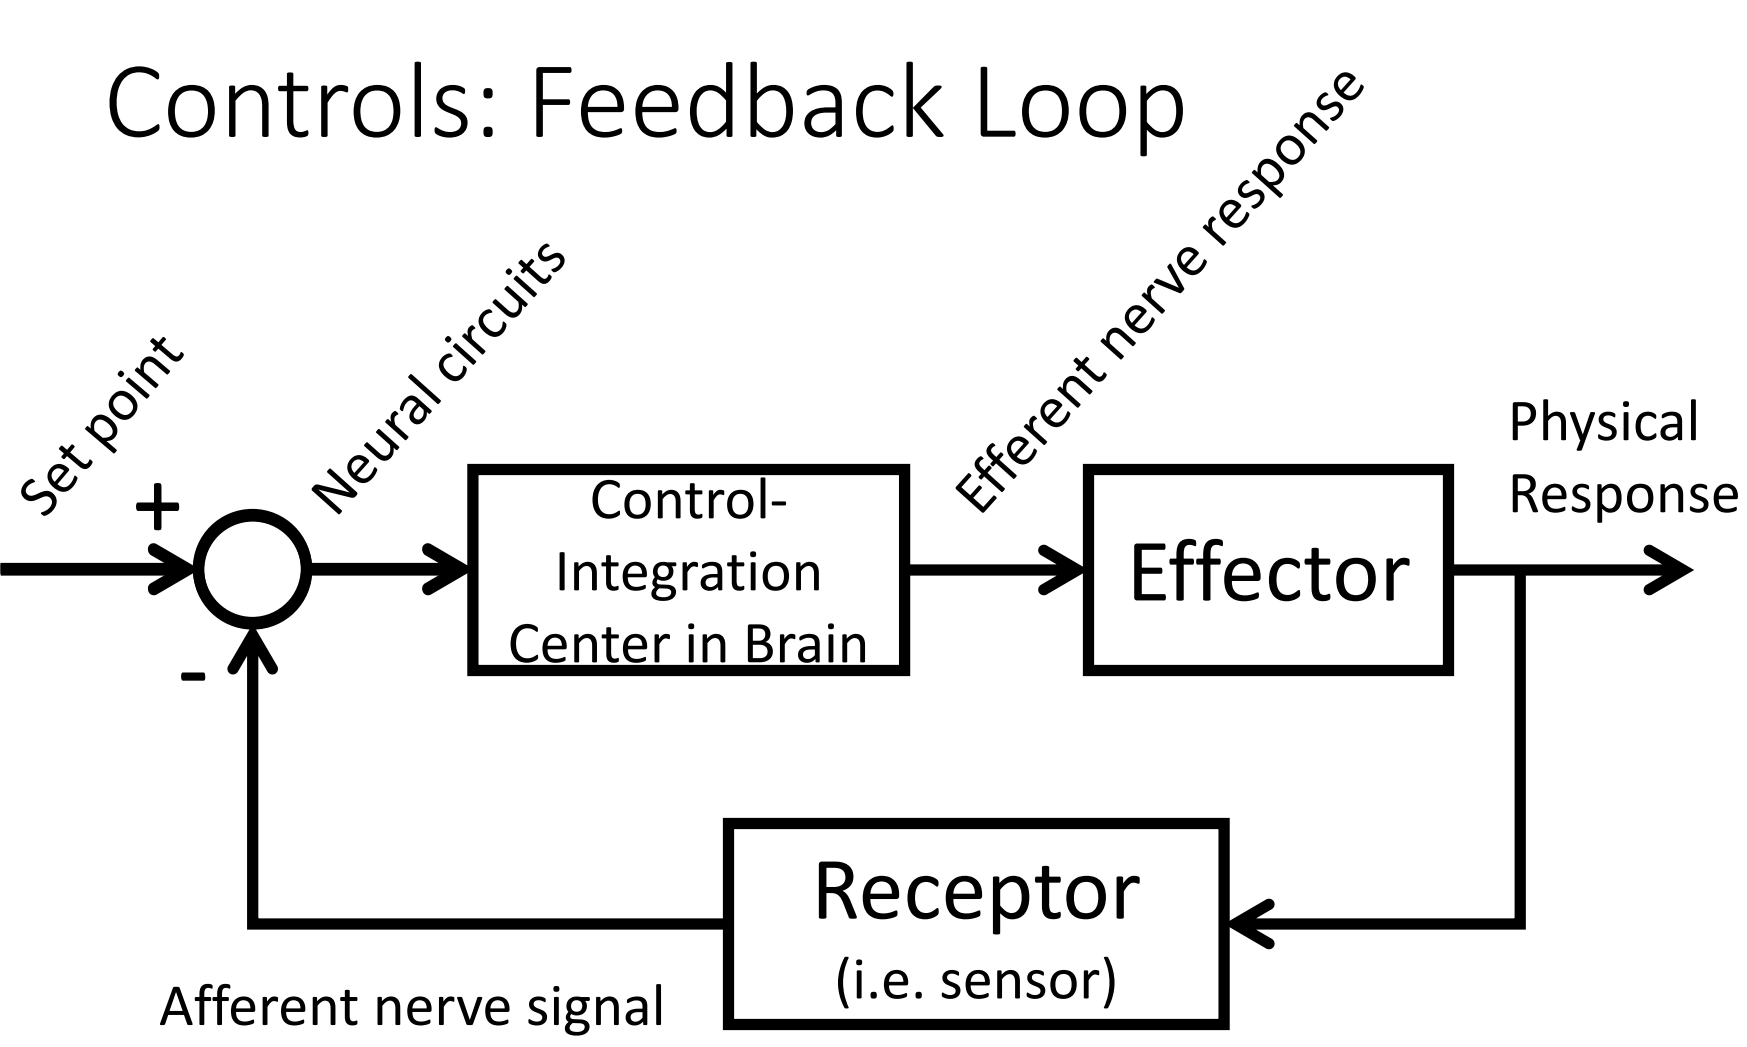
\includegraphics[width=0.65\linewidth]{Pictures/Screenshot 2024-02-25 175821.png}
\end{center}
\begin{exercise}
    For any feedback loop, recognize:
    \begin{enumerate}
        \item physiological variable: \textcolor{blue}{eg. body temp}
        \item sensor: \textcolor{blue}{eg. skin}
        \item control centre in the brain: \textcolor{blue}{eg. hypothalamus, thalamus}
        \item effectors: \textcolor{blue}{eg. sweat glands}
    \end{enumerate}
\end{exercise}
\begin{exercise}
    Which of these statements best describes negative feedback?
    \begin{enumerate}
        \item \textcolor{blue}{A change in a regulated variable triggers a response by the effector that opposes the change}
        \item The input to a system increases the output, and the output limits its own production by inhibiting the input
        \item It is the main operating principle of most of the body’s homeostatic control mechanisms
    \end{enumerate}
\end{exercise}

\section{Cells and DNA}
\begin{descriptions}
    \item[Nucleus:] membrane enclosed organelle in cell that contains chromosomes
    \item[Nucleolus:] largest organ in nucleus, spherical structure, produces \& assembles cell ribosomes
    \item[Ribosome:] specialized cell organelles that reads mRNA build amino acids which combine to make proteins
    \item[Amino acid:] small molecules that are the building blocks of proteins
    \item[Proteins:] large, complex molecules that perform critical roles in body
    \begin{itemize}
        \item creates structure
        \item excecute functions
        \item regulate and organizes tissues
    \end{itemize}
    \item[Chromosome:] condensed form of chromatin with threadlike structure of nucleic acids and protein in the nucleus carrying genetic information (i.e. genes); proteins (i.e. histones) form the structure of chromasomes
    \item[Chromatin:] disorganized nucleic acids and protein (e.g. histones)
    \item[Nucleosome:] basic repeating sub-unit of chromatin
    \item[Nucleic acid:] complex substance in DNA with molecules made up of nucleotides in linked long chain
    \item[Nucleoside:] a compound (e.g. adenosine or cytidine) commonly found in DNA or RNA, consisting of a purine or pyrimidine base (e.g. nitrogen base) linked to a sugar
    \item[Nucleotide:] basic structural unit of DNA composed of a nucleoside and a phosphate group
\end{descriptions}
\begin{center}
    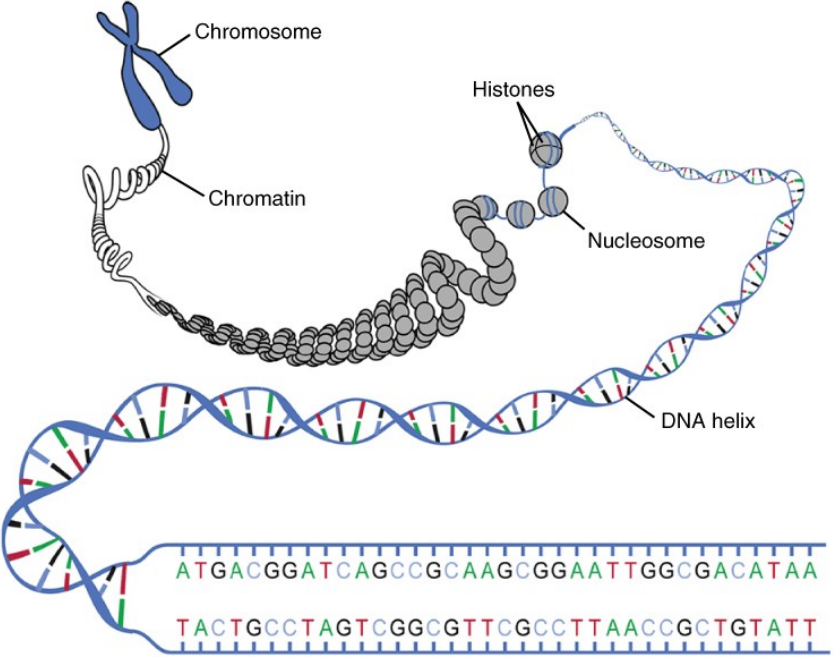
\includegraphics[width=0.65\linewidth]{Pictures/Screenshot 2024-02-25 182833.png}
\end{center}
\subsection{DNA Structure}
\begin{descriptions}
    \item[DNA supercoiling:] the amount of twist in a DNA strand which determines the strainon it
    \begin{itemize}
        \item \textbf{Positive supercoiling:} more tightly twisted
        \item \textbf{Negative supercoiling:} less tightly twisted
    \end{itemize}
    \item[Nucleobase:] one of four amino acids found in DNA (i.e.\textbf{cytosine, thymine, guanine, adenine})
    \item[Base pair:] pair of nucleobases joined by h-bonds (i.e. \textbf{A-T, C-G}). DNA has two c omplementary strands of base pairs
    \begin{itemize}
        \item C: Cytosine
        \item T: Thymine (only in DNA), corresponds to U: Uracil (only in RNA)
        \item A: Adenine
        \item G: Guanine
    \end{itemize}
\end{descriptions}
\begin{exercise}
    Place the following structures in order from least to most complex organization:
    \begin{enumerate}
        \item DNA, nucleosome, chromatin, chromosome
        \item DNA, nucleobase, chromatin, chromosome
        \item \textcolor{blue}{DNA, chromatin, nucleosome, chromosome}
    \end{enumerate}
\end{exercise}
\begin{exercise}
    Which statement correctly describes the organization of DNA in a cell?
    \begin{enumerate}
        \item \textcolor{blue}{DNA is made up of nucleotides and is organized in the form of chromosomes}
        \item DNA is made up of nucleotides and is organized in the form of nucleosomes
        \item DNA is made up of nucleobases and is organized in the form of nucleosomes
        \item DNA is made up of nucleotides and is organized in the form of a double helix
    \end{enumerate}
\end{exercise}

\section{RNA Translation}
\textbf{Deoxyribose} is part of DNA, whereas \textbf{ribose} is part of RNA
\begin{descriptions}
    \item[Transcription:] RNA polymerase reads DNA template one nucleobase at a time and builds an mRNA molecule
    \item[Translation:] Ribosomes decode mRNA and uses information to build a protein (i.e. a chain of amino acids)
\end{descriptions}
\subsection{RNA Structure}
\begin{descriptions}
    \item[Primary structure:] Nucleobase sequence 
    \item[Secondary structure:] H-bonding at different points creates 2D loops, hairpins etc.
    \item[Tertiary structure:] Completed 3D structure of RNA (how it bends, twists etc.)
    \item[mRNA] 
    \begin{itemize}
        \item messenger RNA
        \item formed during transcription
        \item RNA polymerase II
        \item carries the instructions to make proteins
    \end{itemize}
    \item[tRNA]
    \begin{itemize}
        \item transfer RNA
        \item formed during transcription
        \item RNA polymerase III
        \item carries amino acids to the ribosomes
    \end{itemize}
    \item[Ribosomes]
    \begin{itemize}
        \item reads mRNA
        \item receive amino acids from tRNA
        \item synthesize proteins
    \end{itemize}
\end{descriptions} 
\subsection{Codons}
\begin{center}
    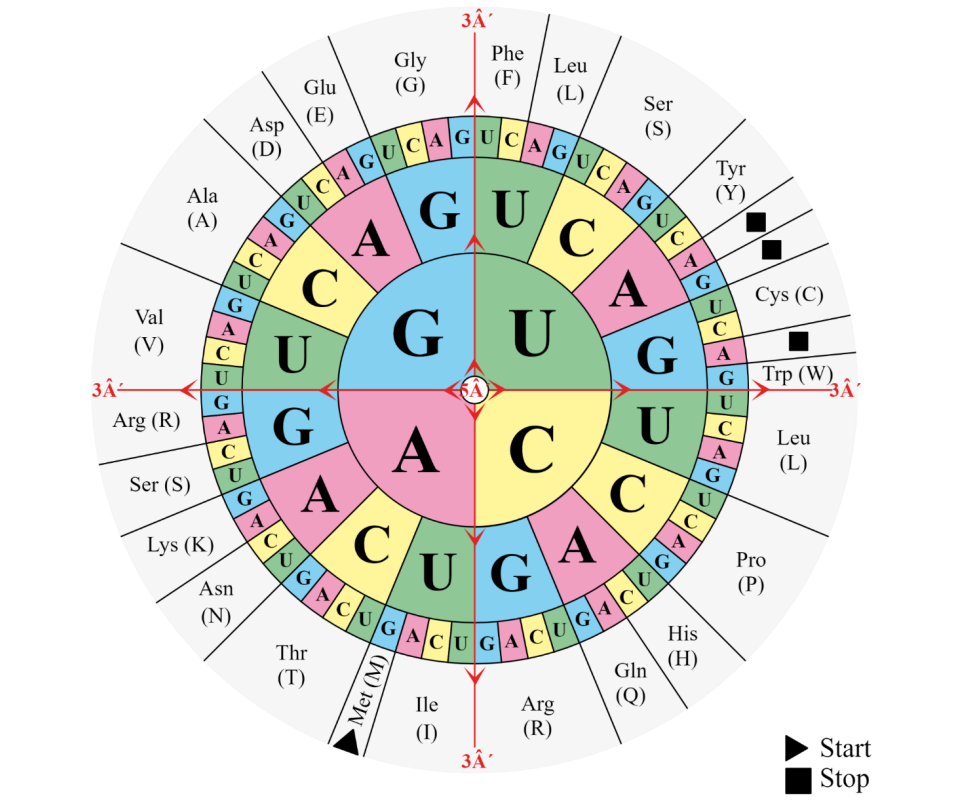
\includegraphics[width=0.65\linewidth]{Pictures/Screenshot 2024-02-25 185241.png}
\end{center}
Codons...
\begin{itemize}
    \item are RNA sequence of 3 nucleotides (i.e. trinucleotide) holding one unit of genomic information
    \item holds instructions for
    \begin{itemize}
        \item encoding a single amino acid \textbf{or}
        \item signalling termination of protein synthesis
    \end{itemize}
\end{itemize}
64 codons exist:
\begin{itemize}
    \item all possible combninations of 4 nucleotides
    \item 61 for amino acids \& 3 stop signals
\end{itemize}
\subsection{Translation}
\subsubsection{tRNA and Amino Acids}
\textbf{Anticodon}
\begin{itemize}
    \item trinucleotide sequence
    \item located at one end of tRNA
    \item corresponds to a complementary codon in mRNA
\end{itemize}
\textbf{tRNA molecure}
\begin{itemize}
    \item 76-90 nuclotides
    \item secondarty structure: clover leaf
\end{itemize}
\textbf{Aminoacyl tNA synthetase}
\begin{itemize}
    \item Enzyme attaching specific amino acid to tRNA
\end{itemize}
\textbf{With tRNA + amino acid}
\begin{itemize}
    \item ready for translation
\end{itemize}
\subsubsection{Initiation}
Reads AUG: the start
\textbf{Pieces for initiation}
\begin{itemize}
    \item ribosome: 2 pieces, large + small
    \item mRNA: instructions to build protein
    \item initiator: tRNA caryying first amino acid, usually Met
\end{itemize}
\textbf{Translation initiation}
\begin{itemize}
    \item tRNA + Met + small ribosome
    \item complex binds to end of mRNA
    \item complex walks down mRNA until reaching the start codon
    \item tRNA + Met bind to start codon
    \item large ribosome joins
\end{itemize}
\textbf{Initiation complex}
\begin{itemize}
    \item tRNA
    \item Met
    \item Small ribosome unit
    \item Large ribosome unit
    \item mRNA
\end{itemize}
\subsubsection{Elongation}
Lengthening of amino acid chain
\begin{itemize}
    \item as each tRNA + amino acid binds to a site mRNA shift forward one codon
    \item new tRNA + amino acid corresponding to exposed codon arrives \& bonds
    \item mRNA shifts forward one codon
    \item process repeats up to 33000 times
\end{itemize}
\subsubsection{Termination}
Ending of translation process
\begin{itemize}
    \item when the exposed coddon (A-site) is a stopping codon termination occurs
    \item release factors in and adds a water moplecure to end of amino acid chain
\end{itemize}

\begin{exercise}
    Why is RNA better suited than DNA for creating proteins?
    \begin{enumerate}
        \item \textcolor{blue}{RNA can leave the nucleus, whereas DNA cannot}
        \item RNA can be easily modified after transcription, whereas DNA cannot
        \item RNA is more stable than DNA
    \end{enumerate}
\end{exercise}
\begin{exercise}
    Which of the following is not made wholly out of RNA?
    \begin{enumerate}
        \item \textcolor{blue}{the ribosome}
        \item the transfer molecule
        \item the messenger molecule that provides the code for protein synthesis
    \end{enumerate}
\end{exercise}
\begin{exercise}
    Which of the following best describes gene expression?
    \begin{enumerate}
        \item The process of copying DNA into RNA
        \item The process of creating proteins from RNA
        \item \textcolor{blue}{The process by which the information in parts of DNA are used to direct the synthesis of proteins and other molecules with specific functions}
    \end{enumerate}
\end{exercise}

\chapter{Transportation and Signal Propagation}
\section{Mitochondria and the Membrane}
A mitochondrion:
\begin{itemize}
    \item is a membrane-bound cell organelle
    \item generates chemicals to power clel biochemical reactions
    \item stores chemical energy in small molucules called \textbf{ATP} (adenosine triphosphate, adenine + ribose + 3 phosphate groups)
\end{itemize}
\begin{center}
    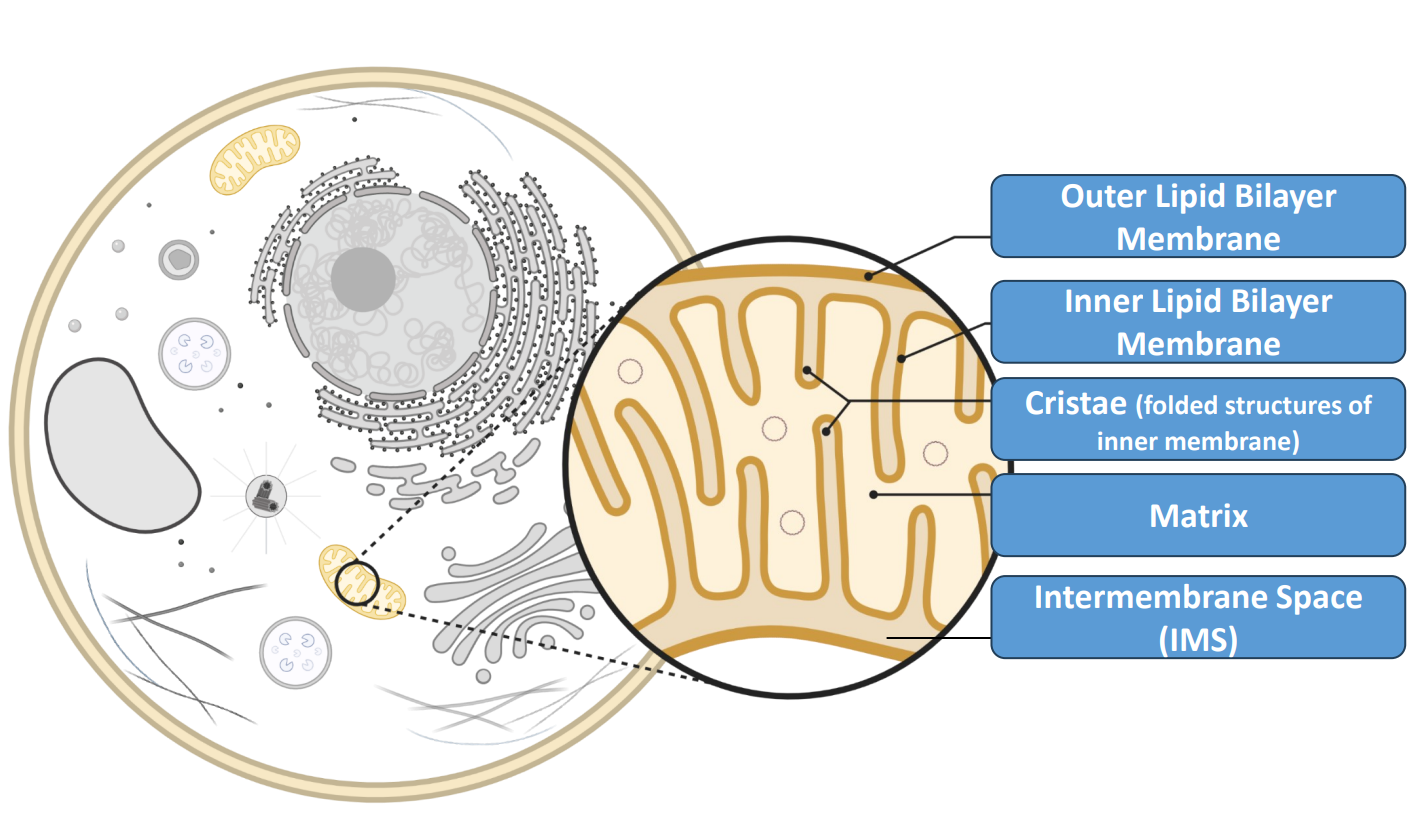
\includegraphics[width=0.65\linewidth]{Pictures/Screenshot 2024-02-25 191455.png}
\end{center}
\subsection{ATP}
How does ATP store energy?
\textbf{High Energy Bonds}
\begin{itemize}
    \item electrons in bond are in high energy state
    \item if bond is broken:
    \begin{itemize}
        \item energy is released
        \item electrons move to low energy state
    \end{itemize}
\end{itemize} 
\subsection{Cellular Respiration}
Cellular respiration is the process of:
\begin{itemize}
    \item combining oxygen with foodstuff molecules
    \item converting this chemical energy into usable form (ATP)
    \item Discarding waste products
\end{itemize}
\textbf{Pathways for ATP Production}
\begin{enumerate}
    \item Glycolysis ($\leq$ 2 ATP)
    \item Pyruvate oxidation
    \item citric acid cycle ($\leq$ 2 ATP)
    \item Oxidative phosphorylation ($\leq$ 34 ATP)
\end{enumerate}
\subsubsection{Cell Membrane}
\textbf{Phospholipid Molecule}
\begin{itemize}
    \item cell membrane consists of a semi-permeable lipid bilayer
    \item phosphate (head, polar \& hydrophilic)
    \item glycerol
    \item fatty acids (tails, non-polar \& hydrophobic)
    \item polar heads of molecules arrange to maximize distance between
\end{itemize}
\begin{center}
    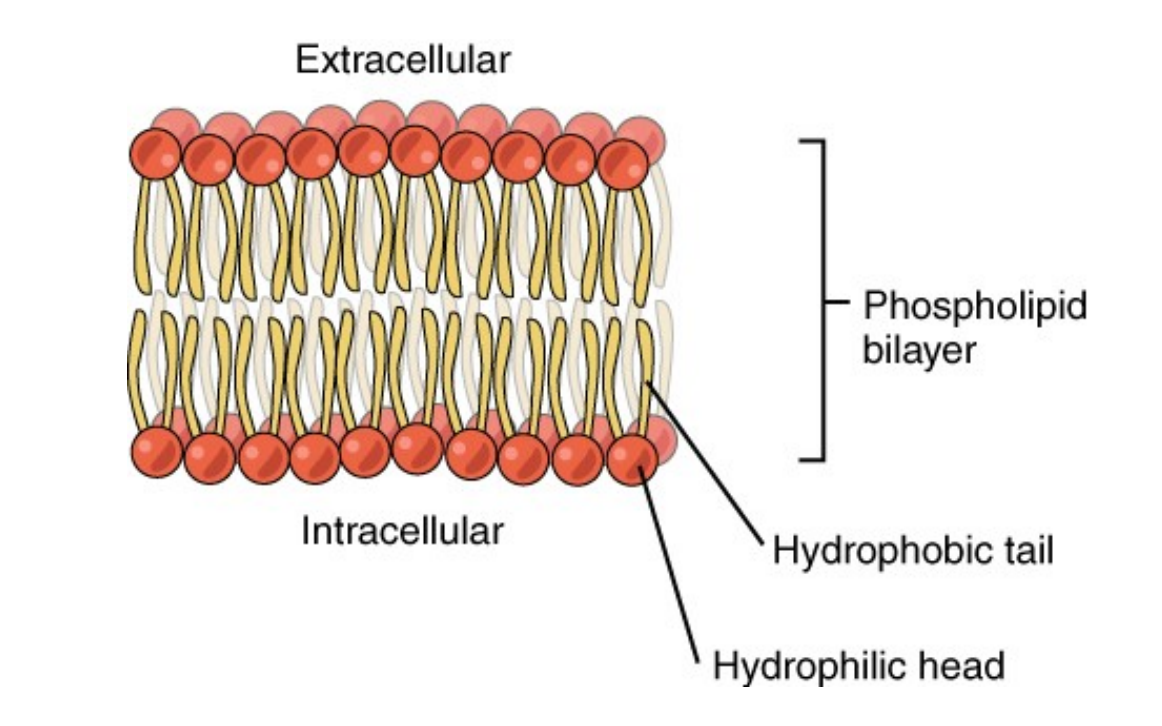
\includegraphics[width=0.65\linewidth]{Pictures/Screenshot 2024-02-25 205202.png}
\end{center}
Note:
\begin{itemize}
    \item channels, pathways, proteins, other lipids etc. all can exist in cell membrane
    \item different components perform different functions
    \item cell membrane passage in/out of cell (e.g. security at a concert)
    \item fat soluble, hydrophobic, non-polar molecules cross quickly
\end{itemize}
\textbf{Permeability}
\begin{itemize}
    \item \textbf{Permeability coefficient:} describes rate of movement through cell membrane
    \item Generally, the the smaller the molecule \& more fat-soluble(i.e. the more nonpolar), the more rapidly it will diffuse across a lipid bilayer
\end{itemize}
\subsubsection{Membrane Transport}
\begin{descriptions}
    \item[Unassisted Membrane Transport (passive diffusion)]\begin{descriptions}
    \end{descriptions}
    \begin{itemize}
        \item molecule (small uncharged molecules/\textbf{concentration gradient}) dissolves into phospholipid bilayer
        \item molecule diffuses across bilayer
        \item molecule dissolves in aqueous solution on opposite side of bilayer
        \item does not require energy, molecules move down concentration gradient
        \item small, uncharged, nonpolar molecules easy to diffuse whereas charged molecules difficult to diffuse
    \end{itemize}
    \item[Assisted Membrane Transport (facilitated diffusion)]\begin{descriptions}
    \end{descriptions}
    \begin{enumerate}
        \item Channel mediated
        \begin{itemize}
            \item particles $\leq$0.8nm
            \item channel proteins are hydrophilic tunnels across membrane
            \item allow polar/charged compounds to avoid hydrophobic core of membrane
            \item \textbf{aquaporins:} channel proteins to speed up crossing of water
            \item some channels open always, others open or close in response to signals (gated)
        \end{itemize}
        \item Carrier mediated
        \begin{itemize}
            \item particles that cannot cross channels
            \item carrier proteins can change shape to move molecules across membrane
            \item slower movement than channels
            \item ion pumps are important example(e.g. ${\rm Na^+-K^+}$ pump)
        \end{itemize}
    \end{enumerate}
    \item[Primary Active Transport (carrier mediated)]\begin{descriptions}
    \end{descriptions}
    \begin{enumerate}
        \item energy source: ATP
        \item cytoplasmic ${\rm Na^+}$ binds to the ${\rm Na^+/K^+}$ pump
        \item the ${\rm Na^+/K^+}$ pump is phosphorylated by ATP
        \item the pump changes its conformation, causing ${\rm Na^+}$ to release
        \item extracellular ${\rm K^+}$ binds to the pump, leading todephosphorylation
        \item the pump returns to its original conformation
        \item ${\rm K^+}$ is released from the pump
    \end{enumerate}
    \item[Secondary Active Transport (channel mediated)]\begin{descriptions}
    \end{descriptions}
    \begin{itemize}
        \item energy source: electrochemical gradient
        \item primary active transport creates electrochemical gradients which store energy
        \item energy in gradient can then be used to push/pull substances across membrane
        \item secondary active transport involves simultaneous transport of ions (e.g. Na) down their gradient \& transport of other substances by co-transporters
        \item \textbf{symporters:} all crossings occur in the same direction
        \item \textbf{antiporters:} crossings occur in opposite directions
    \end{itemize}
\begin{center}
    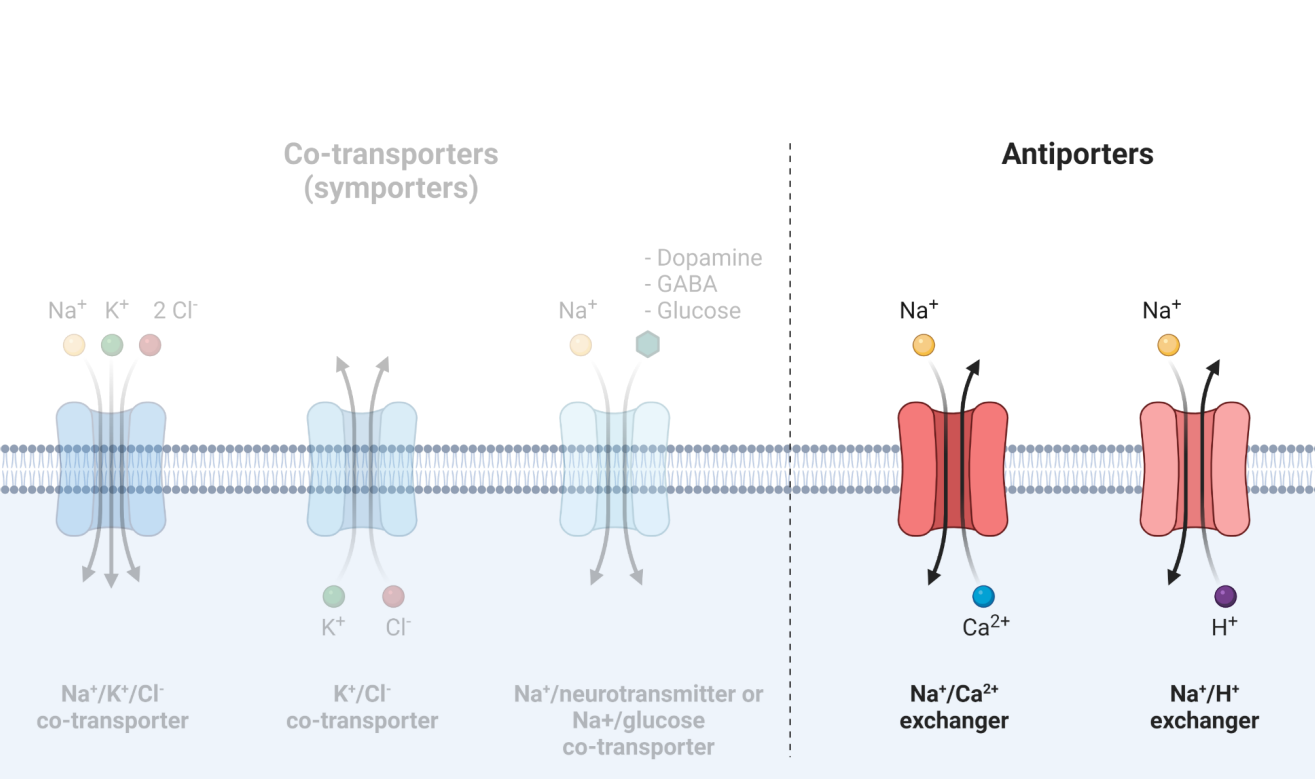
\includegraphics[width=0.65\linewidth]{Pictures/Screenshot 2024-02-25 211519.png}
\end{center}
\begin{exercise}
    Which of the following is not a function of the cellular membrane?
    \begin{enumerate}
        \item Creates distinct outer structure of cell
        \item Facilitates crossing of various molecules, ions, etc.
        \item \textcolor{blue}{Divides the cell into discrete compartments}
    \end{enumerate}
\end{exercise}
\begin{exercise}
    Which of the following are components of the cell membrane?
    \begin{enumerate}
        \item Proteins and phospholipids (i.e. nucleotides, fatty acids)
        \item \textcolor{blue}{Proteins and phospholipids (i.e. glycerol, phosphates, fatty acids)}
        \item Lipid bilayers, cristae, and a matrix
    \end{enumerate}
\end{exercise}
\begin{exercise}
    Which best describes primary active transport?
    \begin{enumerate}
        \item Proteins and phospholipids (i.e. nucleotides, fatty acids)
        \item \textcolor{blue}{Carrier proteins pull molecules across the cell membrane with the assistance of ATP to create electrochemical gradients}
        \item Protein channels facilitate simultaneous movement of ions down their electrochemical gradient
    \end{enumerate}
\end{exercise}
\end{descriptions}

\section{Resting Membrane Potential}
\textbf{Transport Across Membranes}
\begin{itemize}
    \item Key mechanism by which life exists
    \begin{itemize}
        \item allows oxygen and carbon dioxide movement
        \item facilitates nerve conduction (e.g. ion movement \& biosignals)
        \item feeds cell \& life functions (e.g. glucose)
    \end{itemize}
    \item Ion movement
    \begin{itemize}
        \item primary active: \enquote{pumps}
        \item secondary active: \enquote{leakage channels}
    \end{itemize}
\end{itemize}
\textbf{Model vs. Reality}
\begin{itemize}
    \item Single protein 2-pore concept is a simp0lified model
    \item e.g. reality of ${\rm K^+}$ channels
    \begin{itemize}
        \item family of 15 members \enquote{two-pore-domain} channels
        \item each encoded by a unique gene
        \item regulated by multiple mechanisms
        \begin{enumerate}
            \item signalling lipids
            \item oxygen tension
            \item pH
            \item mechanical stretch
            \item G-proteins
        \end{enumerate}
    \end{itemize}
\end{itemize}
\textbf{Voltage Clamp Technique}
\begin{itemize}
    \item electrophysiology: study of electrical properties of cells and tissues
    \item revealed ion channel events of nerve conduction
\end{itemize}
\subsection{Path-Clamp Recording}
\begin{itemize}
    \item facilitate measure of a cell, piece of cell wall or even a single ion channel
    \item study of nerve \& muscle signalling, function, dysfunction, disease
    \item clamper circuits:
    \begin{itemize}
        \item fix voltage and measure current
        \item fix current and measure voltage
    \end{itemize}
    \item 
\end{itemize}
\begin{center}
    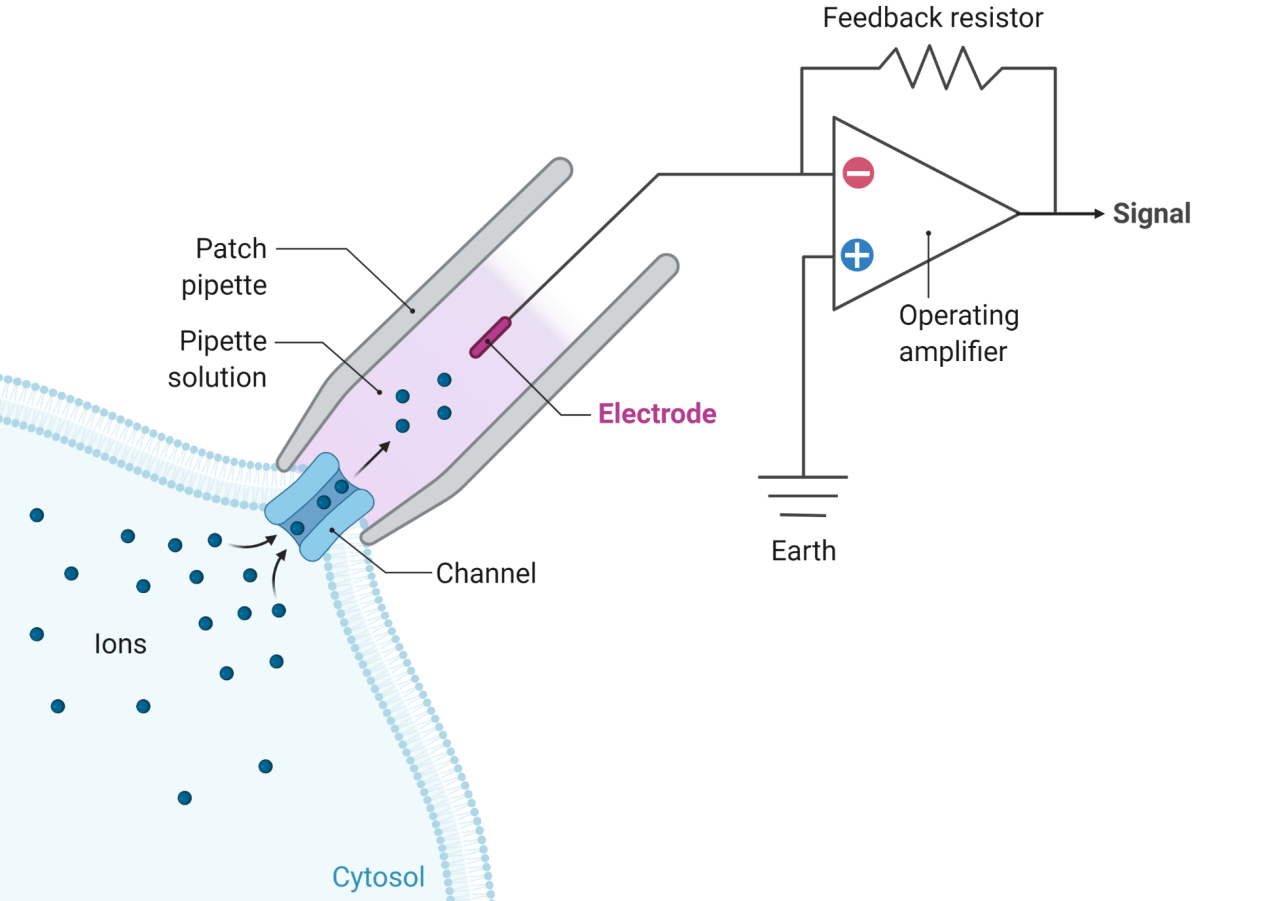
\includegraphics[width=0.65\linewidth]{Pictures/Screenshot 2024-02-25 214256.png}
\end{center}
\begin{itemize}
    \item Single ion channel moves ~10 million ions per second
    \item Resulting current is several picoAmps
    \item Measurement at this physical size \& current range is Very challenging
    \item Thin pipette ($\approx$1um) contacts membrane
    \item Suction applied to create high-resistance seal(G$\Omega$)
    \begin{itemize}
        \item Physically \& electrically isolates patch of cell
        \item All ions through channel flow into pipette
    \end{itemize}
    \item Solution mimicking extracellular or intracellular (e.g. cytoplasm) environment placed in pipette
    \item Ag/AgCl electrodes
    \begin{itemize}
        \item 1 placed in pipette
        \item 1 placed as reference
    \end{itemize}
    \item Electrodes connected to voltage clamping circuits
    \begin{itemize}
        \item Ion flow changes directly reflected in current measurements
    \end{itemize}
\end{itemize}

\subsection{Nerst Equation}
\begin{theorem}
    $$E_x=\frac{R_uT}{Z_xF}\log_{10}\frac{[C]_0}{[C]_i}=\frac{61}{Z_x}\log_{10}\frac{[C]_0}{[C]_i}$$
    where
    \begin{itemize}
        \item $E$ is equilibrium potential in $mV$
        \item $x$ is ion
        \item $Z$ is charge
        \item $[C]_0$ is concentration outside cell
        \item $[C]_i$ is concentration inside cell
        \item $R_u,T,F$ are gas constant, temperature @36.5$^\circ C$ and Faraday constant respectively
    \end{itemize}
    \textbf{Equilibrium potential:} differential at equilibrium across membrane due to ion concentration gradient
\end{theorem}

\subsection{Goldman-Hodgkin-Katz (GHK) Equation} 
\begin{theorem}
    $$V_m = \frac{RT}{ZF} \ln \left(\frac{P_{Na}[Na]_o + P_K[K]_o + P_{Cl}[Cl]_i}{P_{Na}[Na]_i + P_K[K]_i + P_{Cl}[Cl]_o} \right)$$
    where
    \begin{itemize}
      \item $V_m$ is the membrane potential (mV)
      \item $R$ is the universal gas constant (8.314 J/mol K)
      \item $T$ is the absolute temperature (K)  
      \item $F$ is the Faraday constant (96485 C/mol)
      \item $P_{Na}$, $P_K$, $P_{Cl}$ are the permeabilities of Na+, K+, and Cl- ions
      \item $[Na]_o$, $[K]_o$, $[Cl]_o$ are the outside concentrations of Na+, K+, and Cl- ions
      \item $[Na]_i$, $[K]_i$, $[Cl]_i$ are the inside concentrations of Na+, K+, and Cl- ions
    \end{itemize}
    \textbf{Membrane potential:} potential difference across a cell membrane that accounts for ion concentrations and permeabilities. \textbf{Resting membrane potential} is usually approximately -70 mV
\end{theorem} 
\begin{remark}
    \textbf{Note that} $E_{\rm ion}\neq V_m$
\end{remark}

\subsection{Graphing Electrochemical Gradients}
\begin{enumerate}
    \item Set up graph with the Electrical Driving Force (V) on y-axis and Concentration Driving Force on the x-axis
    \item Write concentration inside \& outside cell
    \item Mark an ‘X’ on the side of the x-axis that the concentration gradient moves the ion
    \item mark an ‘X’ where E is on y-intercept
    \item Draw line between two ‘X’s
    \item Determine what the ion will do at the V
\end{enumerate}
\begin{center}
    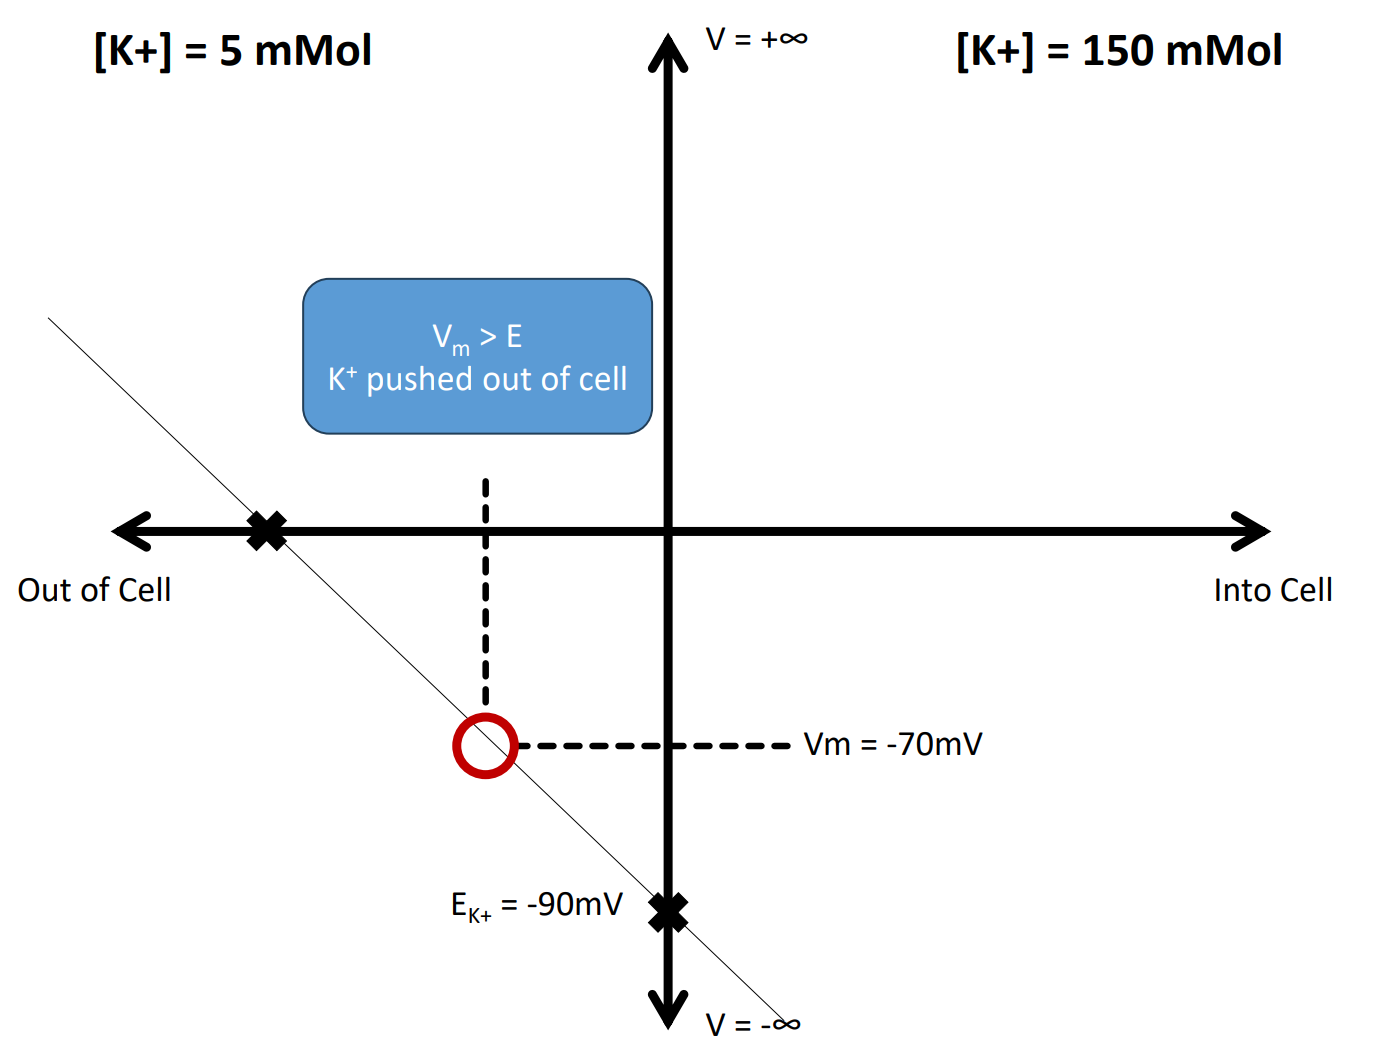
\includegraphics[width=0.65\linewidth]{Pictures/Screenshot 2024-02-25 220308.png}
    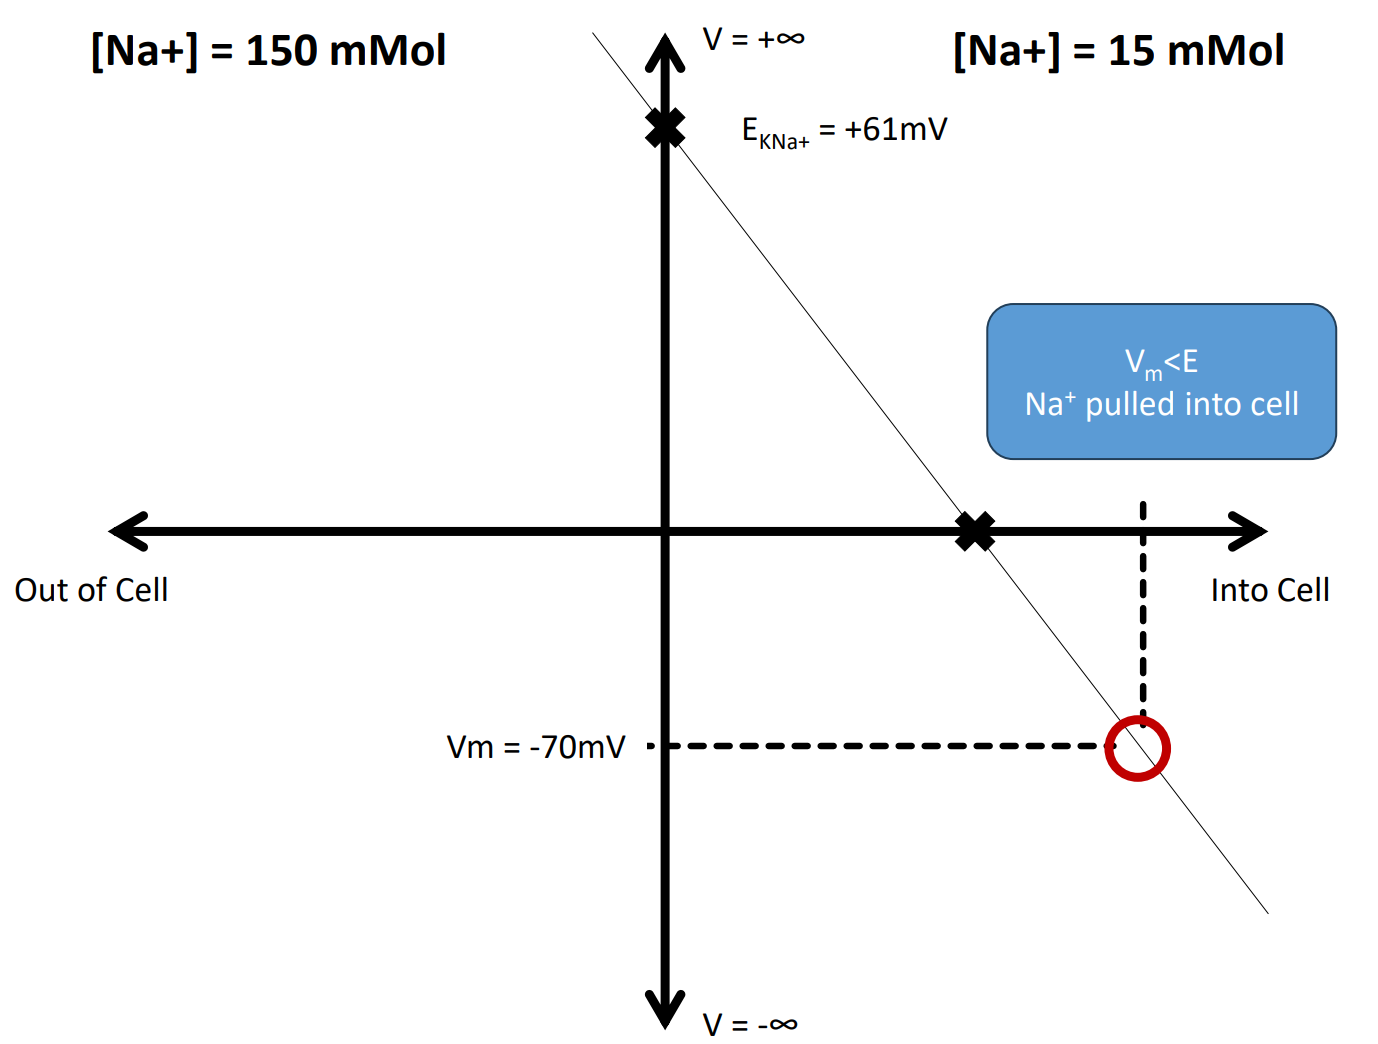
\includegraphics[width=0.65\linewidth]{Pictures/Screenshot 2024-02-25 222320.png}
\end{center}
\subsection{Gibbs Free Energy}
\begin{theorem}[Equilibrium Potential Balances: Diffusion and Electrical Potential]
    $$\Delta G_{\rm chem}=RT\ln\frac{[C]_o}{[C]_i},\;\Delta G_{\rm elec}=ZFV_m$$
    where at equilibrium,
    $$\Delta G_{\rm chem}=\Delta G_{\rm elec}$$
\end{theorem}
\begin{proposition}[Free Energy Moving Out of a Cell]
    $$\Delta G=\Delta G_{\rm chem}-\Delta G_{\rm elec}$$
    If $\Delta G < 0$, movement is spontaneous\\
    If $\Delta G > 0$, movement is not spontaneous
\end{proposition}

\section{Action Potential}
\begin{descriptions}
    \item[Depolarization:] rapid rise in membrane potential due to a large influx of positive ions
    \item[Repolarization:] rapid decrease in membrane potential towards the resting membrane potential due to a large efflux of positive ions
    \item[Hyperpolarization:] lowered membrane potential below resting membrane potential due to a large efflux of positive ions 
\end{descriptions}
\begin{center}
    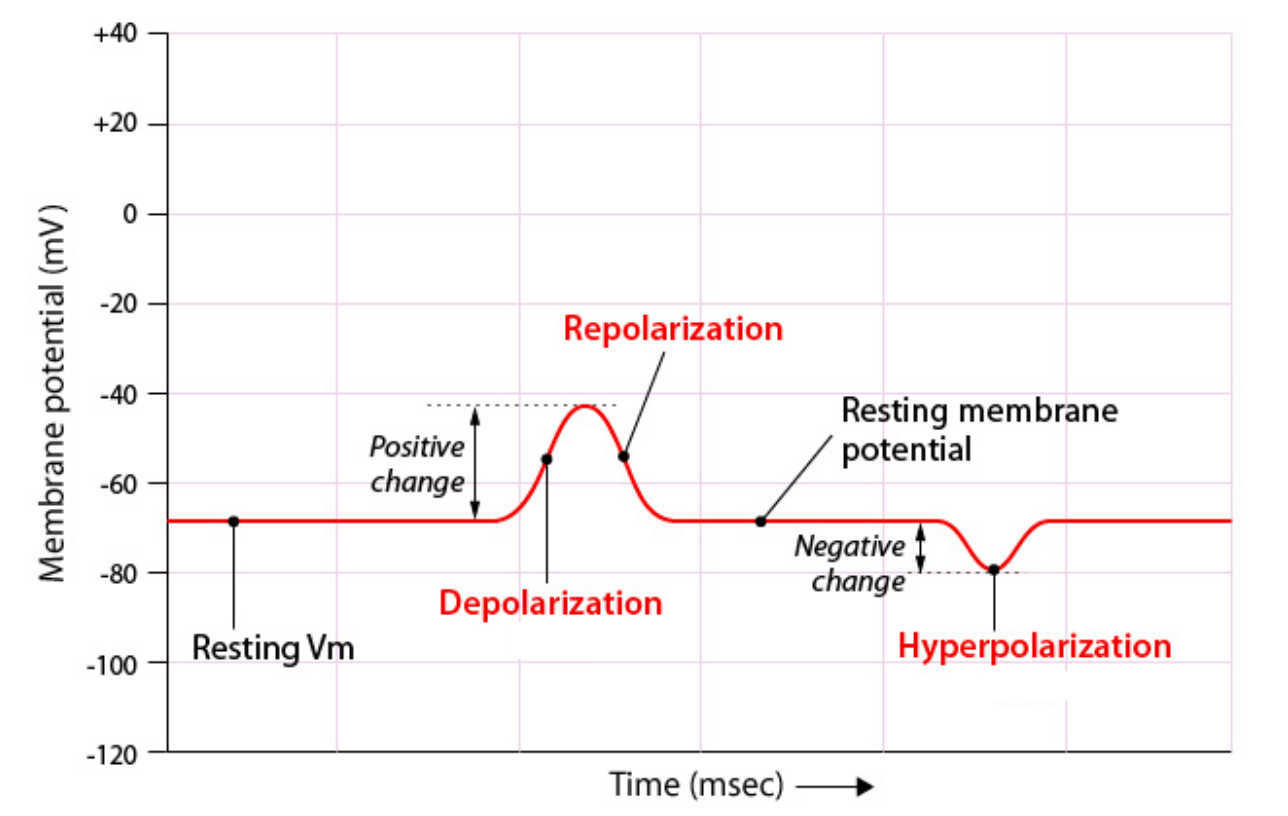
\includegraphics[width=0.65\linewidth]{Pictures/Screenshot 2024-02-25 223612.png}
\end{center}
\subsection{Gated Ion Channels}
\begin{descriptions}
    \item[Carrier Mediated Proteins]\begin{descriptions}
    \end{descriptions} 
    \begin{itemize}
        \item ion pumps
        \item contribute to maintaining resting membrane potential
    \end{itemize}
    \item[Ungated Channels]\begin{descriptions}
    \end{descriptions}    
    \begin{itemize}
        \item leak channels (approx. constant permeability)
        \item contribute to maintaining resting membrane potential
    \end{itemize}
    \item[Gated Channels]\begin{descriptions}
    \end{descriptions}
    \begin{itemize}
        \item \textbf{ligand-gated} (chemically gated): open/close state determined by binding of chemical ligand
        \begin{itemize}
            \item ligands are neutral molecules or ions
            \item binds to central atom or ion
            \item water, ammonia, carbon monoxide, chloride, hydroxide are examples
        \end{itemize}
        \item \textbf{voltage gated}: open/close state determined by membrane potential
        \item \textbf{mechanically gated}: open/close state determined by mechanical loading
    \end{itemize}
\end{descriptions}
\subsection{Graded Potentials}
\subsubsection{Neuron Structure}
\begin{center}
    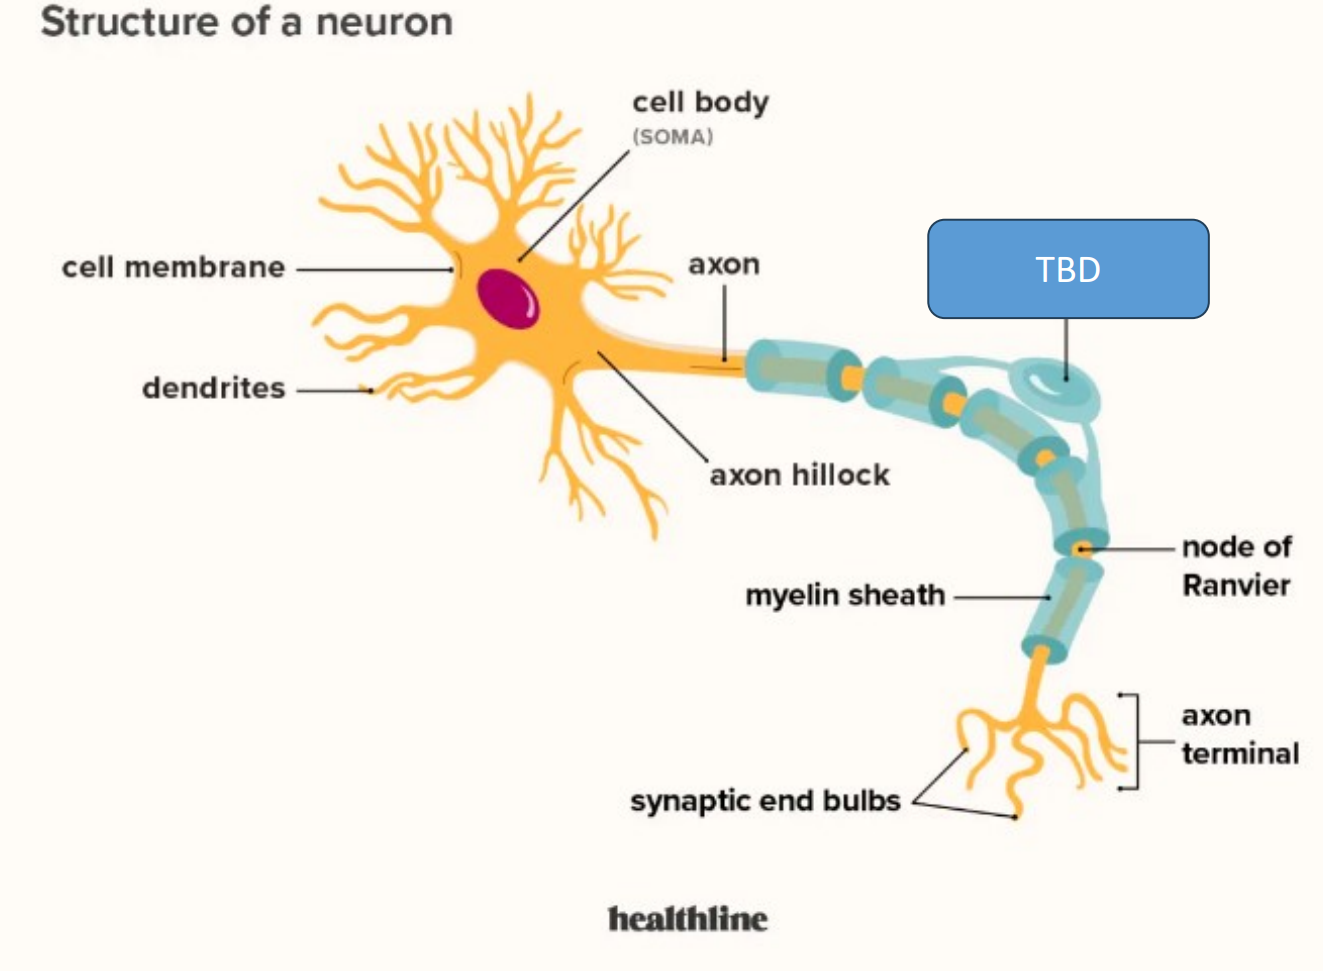
\includegraphics[width=0.65\linewidth]{Pictures/Screenshot 2024-02-25 224731.png}
\end{center}
\begin{itemize}
    \item Soma and dendrites typically at resting membrane potentials of -70 mV
    \item Inputs from certain stimuli can increase (depolarize) or decrease (hyperpolarize)
    \item Transient changes to membrane potential at soma/dendrites
    \item Do not pass into axons of most neurons
    \item Size \& duration determined by size \& duration of stimulus
\end{itemize}
\subsubsection{Propagation of Graded Potential}
\begin{itemize}
    \item system begins at resting membrane potential
    \item stimulus triggers opening of gated ion channel
    \item eg. $\rm{Na^+}$ channel opens \& $\rm{Na^+}$ ions flow into cell
    \item depolarization begins at gated channel
    \item adjacent regions of cell membrane are at resting membrane potential still
    \item current starts to flow along cell membrane (i.e. differential)
    \item depolarization spreads
    \item graded potentials don't spread into axon
\end{itemize}
\subsection{Action Potentials}
\begin{itemize}
    \item graded potentials propagate to axon hillock and then die
    \item once potential reaches threshold at axon hillock action potential is triggered
\end{itemize}
\begin{center}
    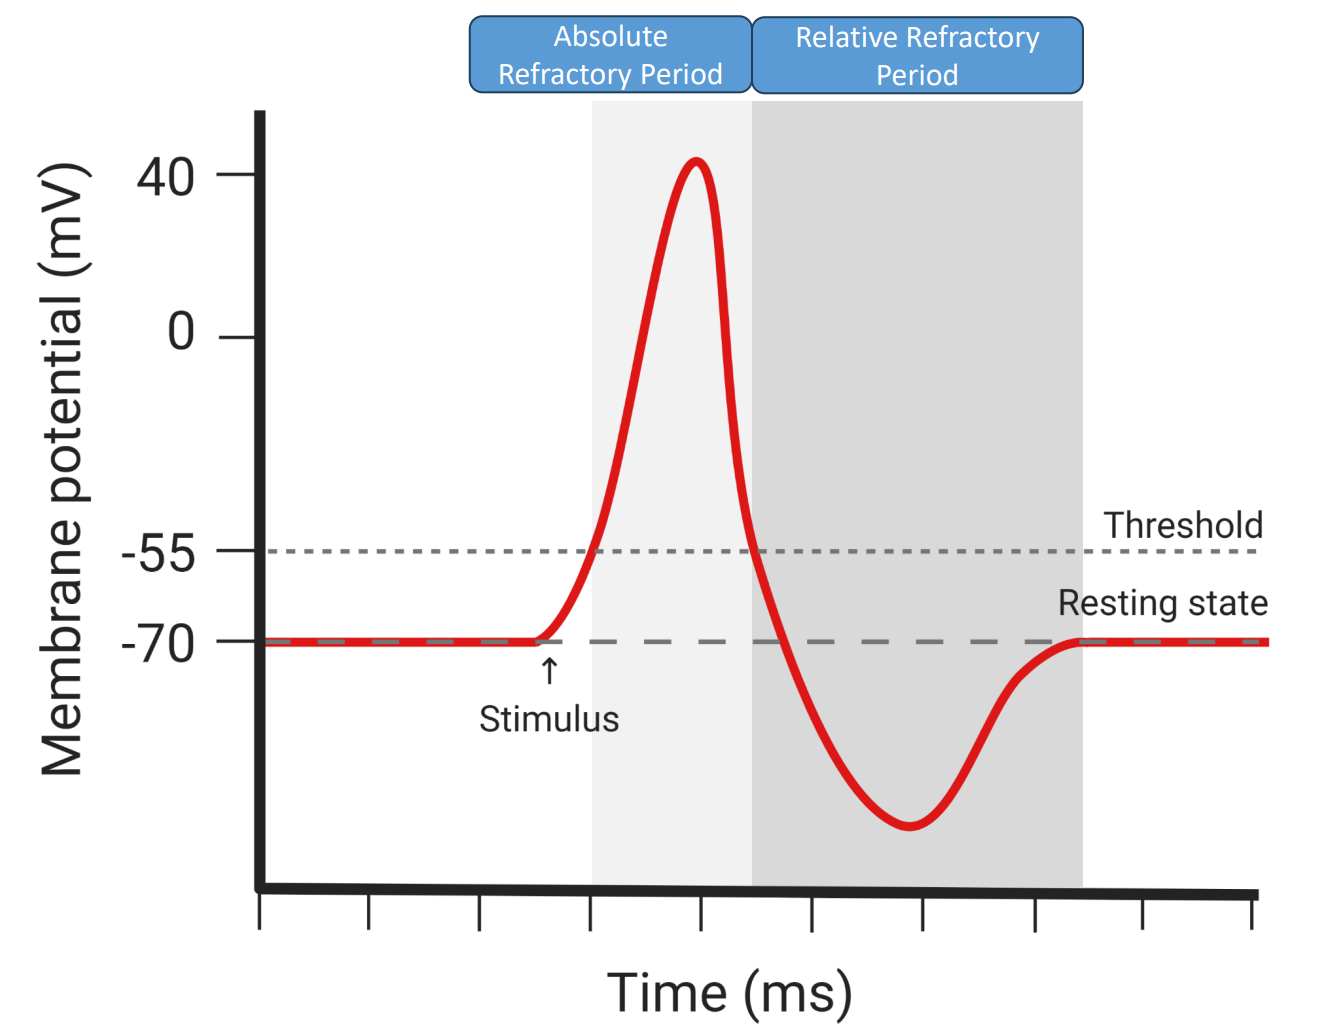
\includegraphics[width=0.65\linewidth]{Pictures/Screenshot 2024-02-26 003521.png}
\end{center}
\begin{descriptions}
    \item[Contiguous conduction:] 
    \begin{descriptions}
    \end{descriptions}    
    velocity between 0.5 and 2 $m/s$
    \item[Saltatory conduction:] 
    \begin{descriptions}
    \end{descriptions}    
    velocity between 100 and 300 $m/s$ 
    \item[Myelin sheath]\begin{descriptions}
    \end{descriptions} 
    \begin{itemize}
        \item insulates axon
        \item assembles voltage gated channel clusters at discrete notes
        \item signal jump between nodes of Ranvier
        \item \textbf{Schwann cells:} myelin production, maintenance, repair
    \end{itemize}
    \item[Factors that affect speed of propagation]\begin{descriptions}
    \end{descriptions} 
    \begin{itemize}
        \item amount of myelination
        \item axon diameter
        \item temperature
    \end{itemize}
\end{descriptions}

\section{Synapses}
\begin{descriptions}
    \item[Electrical synapse:] 
    \begin{descriptions}
    \end{descriptions}
    Synapse at which transfer of information (e.g. voltage potential) occurs via direct connection at gap junction
    \begin{itemize}
        \item info relayed through voltage potential
        \item fast but inefficient
        \item signal same or less in post-synaptic neuron (no gain)
        \item urgent response systems (instinct, defense, cardiac)
        \item excitatory response only
        \item Electrical signal in pre-synaptic neuron $\rightarrow$ electrical signal in post-synaptic neuron
    \end{itemize}
    \item[Presynaptic neuron:] 
    \begin{descriptions}
    \end{descriptions}
    Neuron that transmits signal towards synapse
    \item[Gap junction]
    \begin{descriptions}
    \end{descriptions}
    \begin{itemize}
        \item Gap between adjacent neurons (pre- \& post-)
        \item Composed of $\approx$100 intercellular channels called \textbf{connexons}
        \item Connexons are inserted into cell membranes of adjacent neurons
        \item Voltage-gated channels
        \item Open/close state depend on voltage differential between interior of 2 cells
        \item Can be modulated by:
        \begin{itemize}
            \item ${\rm Ca^{2+}}$, though it can block function
            \item protein phosphorylation, though can degrade channels and accumulate clusters of channels via connexin trafficking from golgi apparatus
        \end{itemize}
    \end{itemize}
    \item[Connexons]
    \begin{descriptions}
    \end{descriptions}
    \begin{itemize}
        \item Tunnels (channels) between adjacent neurons made of small proteins
        \item Allow electrical synapse to share information via transfer of ions \& signalling molecules between cells
    \end{itemize}
    \item[Postsynaptic neuron]
    \begin{descriptions}
    \end{descriptions}
    \begin{itemize}
        \item Neuron that transmits signal away from synapse
        \item Interface between synapse of presynaptic neuron \& dendrites of post-synaptic neuron
    \end{itemize}
    \item[Chemical synapse:] 
    \begin{descriptions}
    \end{descriptions}    
    Synapse at which transfer of information occur via release of neurotransmitter
    \begin{itemize}
        \item info relayed through chemicals
        \item slow, sturdy, efficient
        \item signal can increase (gain possible)
        \item less urgent response systems (CNS, perception, thought)
        \item excitatory or inhibitory response
        \item Electrical $\rightarrow$ chemical pre-synaptic neuron $\rightarrow$ Electrical in post-synaptic neuron
    \end{itemize}
    \item[Vesicle]
    \begin{descriptions}
    \end{descriptions}
    \begin{itemize}
        \item Thin walled sac filled with fluid
        \item Structure within or outside of cell containing fluid or cytoplasm enclosed in lipid bilayer
        \item Synaptic vesicles also contain neurotransmitters
    \end{itemize}
    \item[Synaptic cleft]
    \begin{descriptions}
    \end{descriptions}
    \begin{itemize}
        \item Gap between pre- and post- synaptic neuron at a chemical synapse 
        \item Post-synaptic neuron contains ligand-gated channels whose open/close state is controlled by neurotransmitters binding to receptors on channels
    \end{itemize}
\end{descriptions}
\begin{center}
    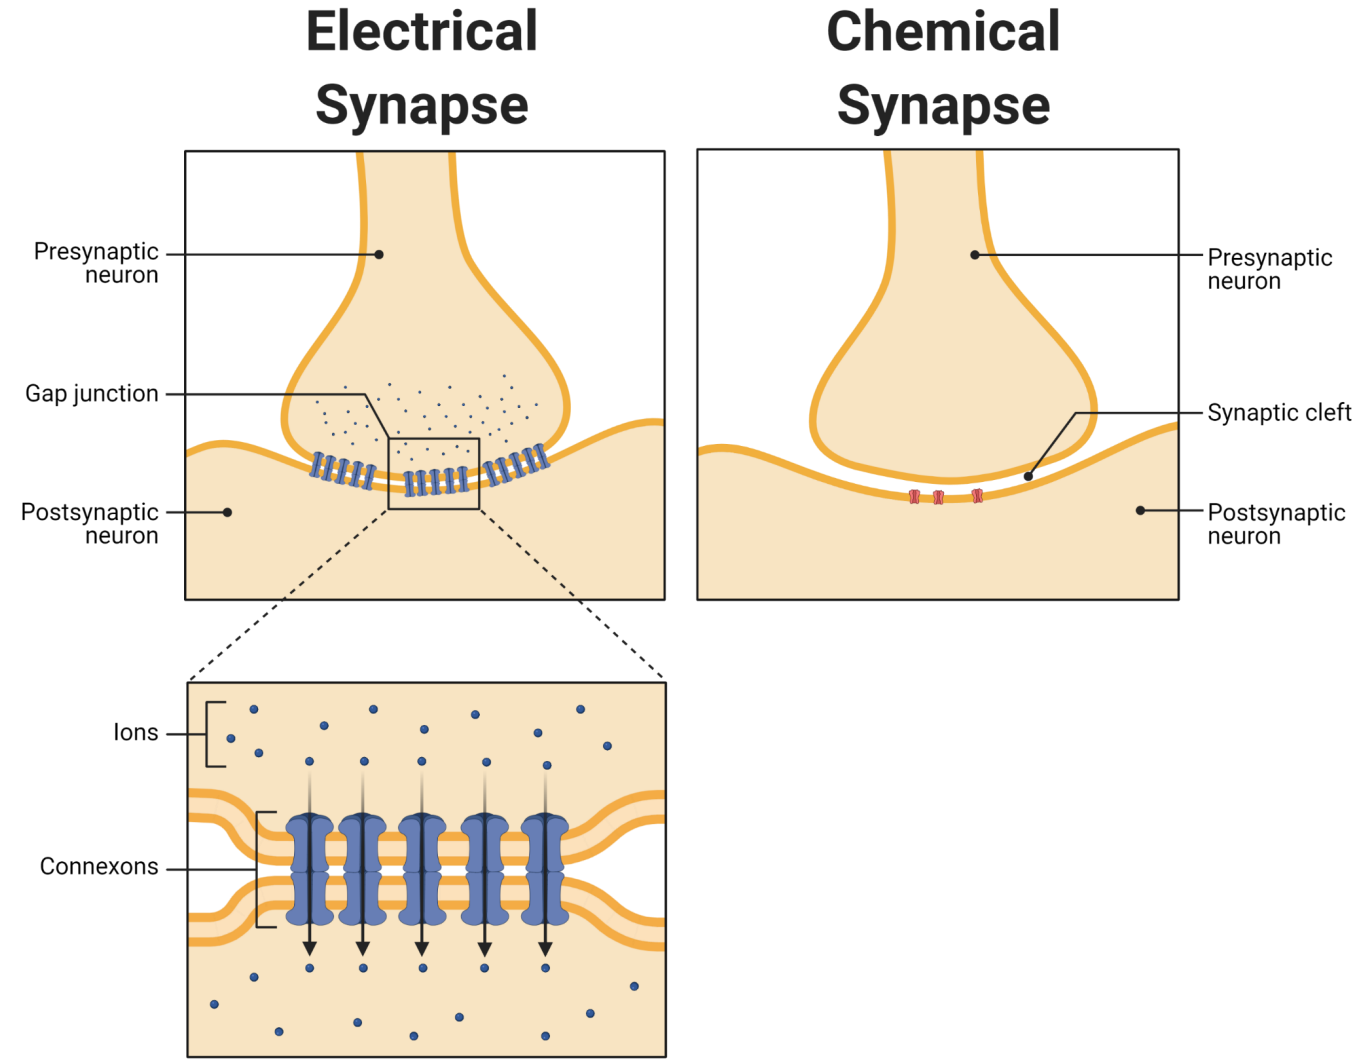
\includegraphics[width=0.65\linewidth]{Pictures/Screenshot 2024-02-26 005340.png}
\end{center}
\begin{remark}
    \textbf{Electrical synapse:} ions transferred from pre-synaptic neuron to post-synaptic neuron. Only \textbf{excitatory}.\\
    \textbf{Chemical synapse:} ions are transferred from extracellular environment to post-synaptic neuron (process triggered by AP). Can be both \textbf{excitatory} and \textbf{inhibitory}.
\end{remark}
\subsubsection{Chemical Synapse Transmission}
\begin{itemize}
    \item neurotransmitters are synthesized and stored in vesicles
    \item action potential arrives at the presynpatic terminal
    \item voltage-gated ${\rm Ca^{2+}}$ channels open, allowing influx of ${\rm Ca^{2+}}$
\end{itemize}
\textbf{Synaptic Vesicle Behavior} 
\begin{itemize}
    \item ${\rm Ca^{2+}}$ ions bind to receptors on vesicles causing them to dock at cell membrane \& release neurotransmitters
    \item ${\rm Ca^{2+}}$ allows vesicle docking and neurotransmitter release
    \item neurotransmitter binds to receptors, causing channels to open or close
    \item excitatory or inhibitory postsynaptic potential is generated
    \item neurotransmitter is removed by glial/neuron uptake or enzymatic degradation
    vesicular membrane is retrieved from the plasma membraneZ
\end{itemize}
\begin{center}
    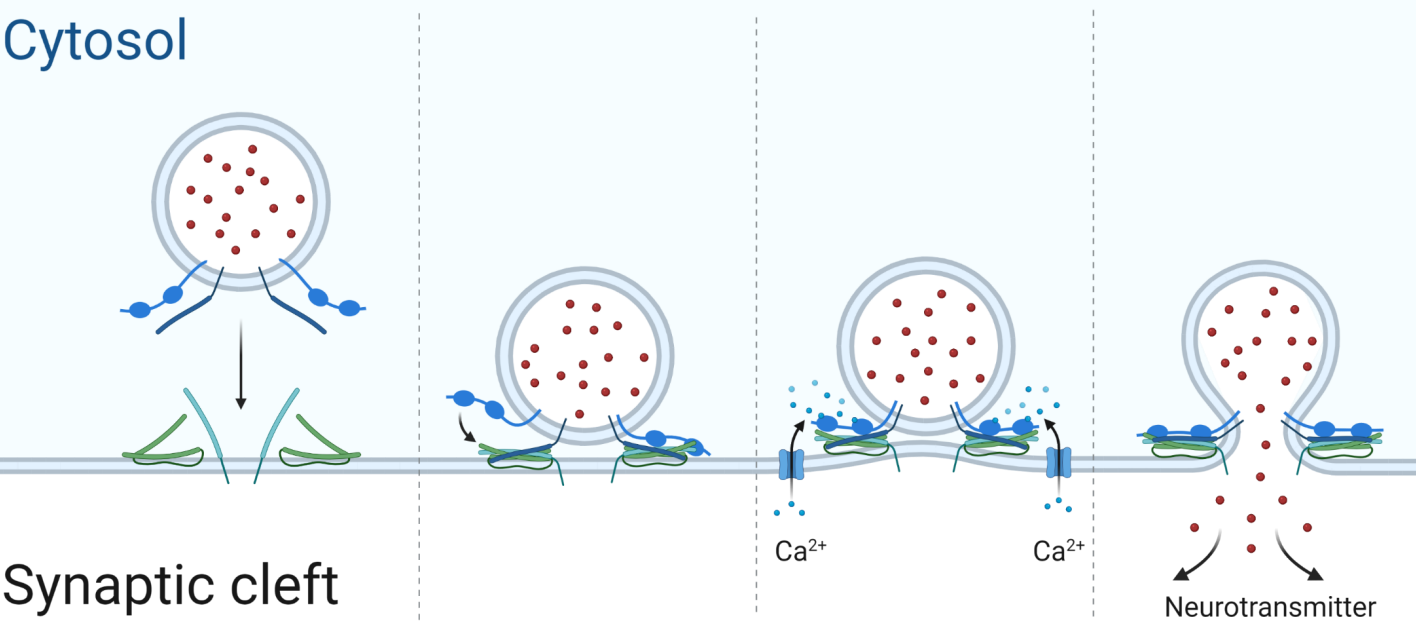
\includegraphics[width=0.65\linewidth]{Pictures/Screenshot 2024-02-26 011050.png}
\end{center}
\begin{center}
    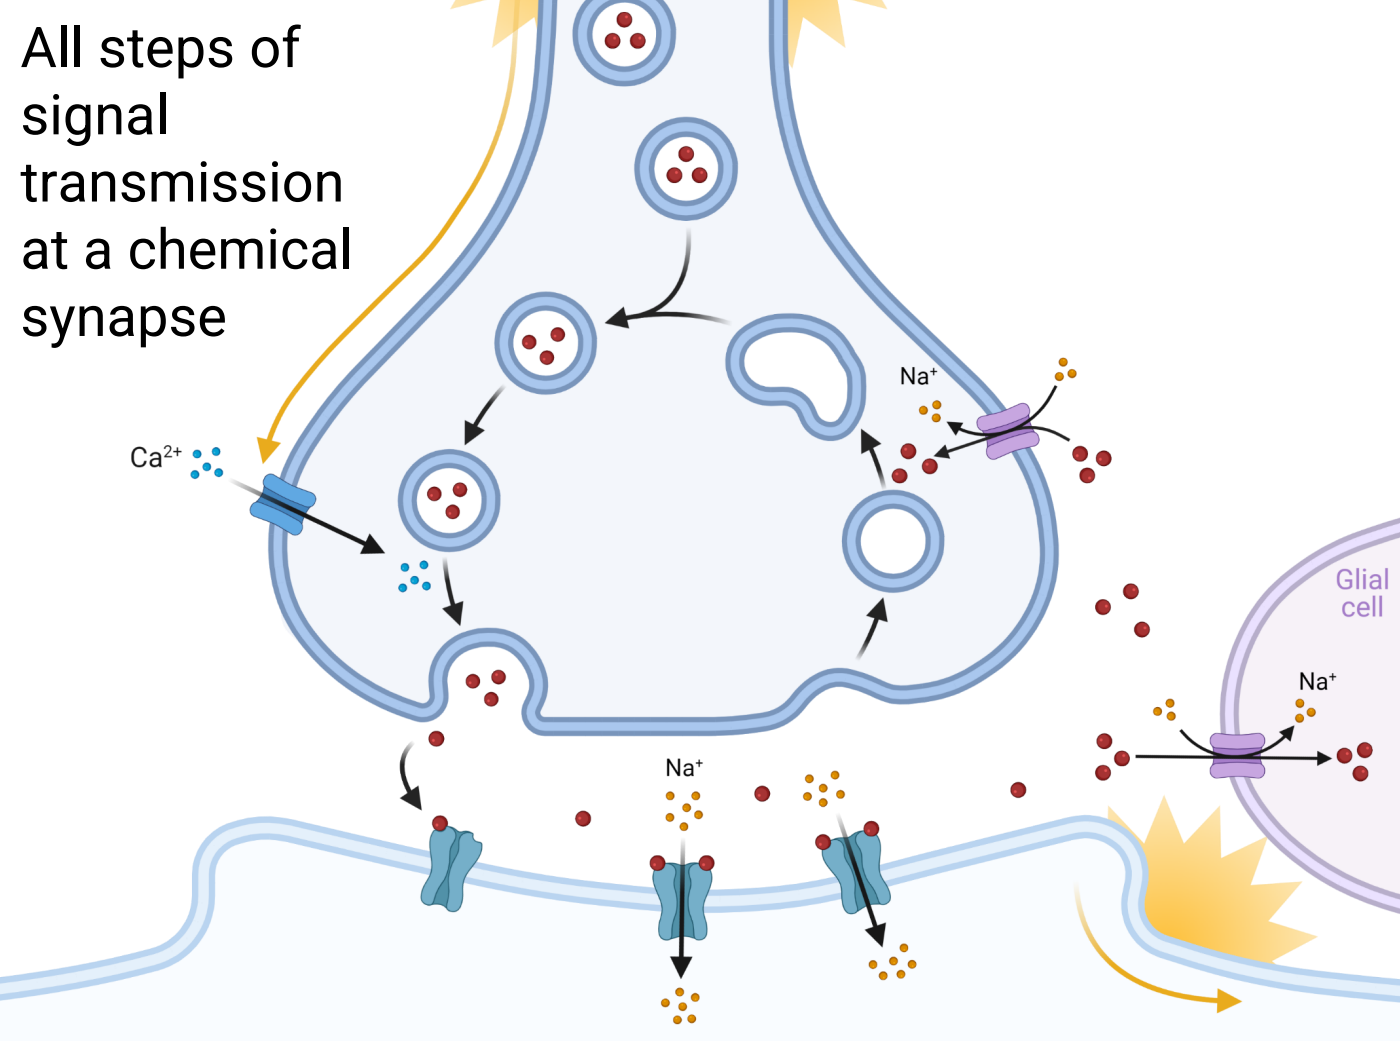
\includegraphics[width=0.65\linewidth]{Pictures/Screenshot 2024-02-26 011404.png}
\end{center}

\begin{descriptions}
    \item[Excitatory PostSynaptic Potential:] potentials that \textbf{depolarize} and increase the likelihood of an action potential
    \item[Inhibitoryy PostSynaptic Potential:] potentials that \textbf{hyperpolarize} and decrease the likelihood of an action potential
\end{descriptions}

\subsection{Excitatory Synapses}
\begin{descriptions}
    \item[Spatial Summation] 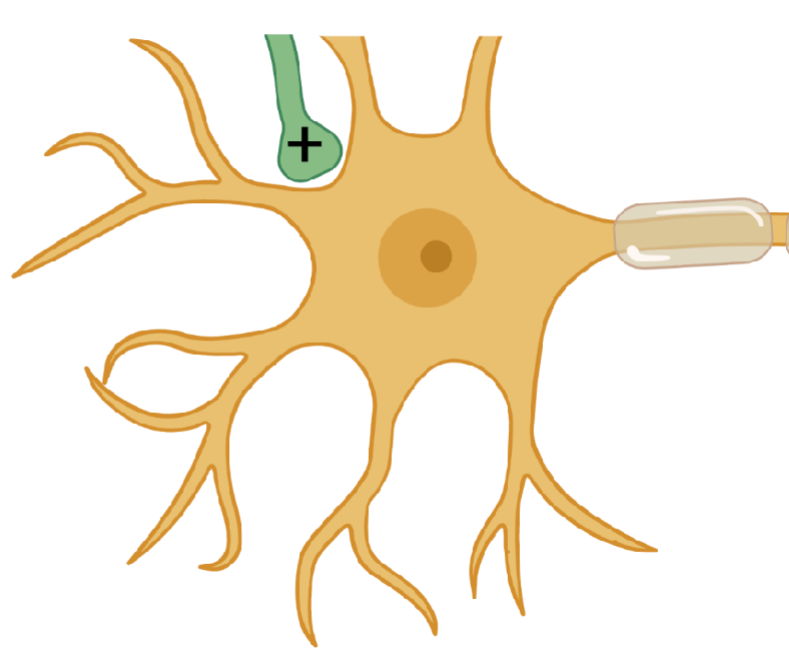
\includegraphics[width=60pt]{Pictures/Screenshot 2024-03-06 175455.png} 
    \item[Temporal Summation] 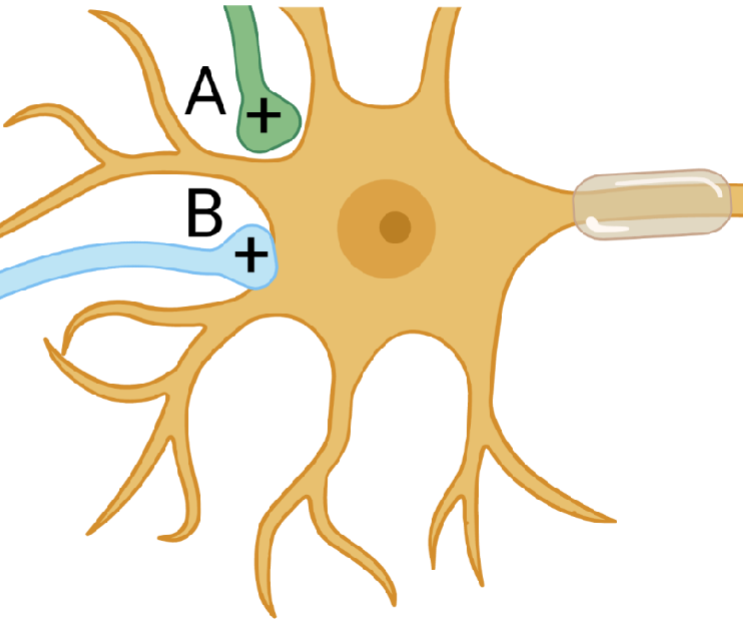
\includegraphics[width=60pt]{Pictures/Screenshot 2024-03-06 175510.png} 
    \item[Grand postsynaptic potential:] combination of all temporal \& spatial summation 
\end{descriptions}

\subsection{Inhibitory Synapses}
\textbf{Postsynapic inhibition}\\
\begin{itemize}
    \item Release of inhibitory neurotransmitter by presynaptic neuron directly inhibits depolarization of postsynaptic neuron
    \item Triggers influx of negatively charged ions (usually ${\rm Cl^-}$) or efflux of positive ions (usually ${\rm K^+}$) and hyperpolarizes postsynaptic neuron  (this dampens a neuron's ability to fire)
    \item May be a single signal (hyperpolarization) or a combined signal(hyper + depol) from multiple synapses in cell body of postsynaptic neuron
    \item Inhibitory neuron synapse at \textbf{axon terminal} of presynaptic neuron indirectly inhibits depolarization of postsynaptic neuron
    \item Inhibitory neuron sends signal and releases neurotransmitters
    \item Neurotransmitters bind to receptors on presynaptic synapse and closes calcium channels (Limits neurotransmitters released from excitatory neuron, so not as many channels open on postsynaptic neuron)
    \item \textbf{Function:} modulates synaptic strength, allows for filtering of sensory information, regulation of neural circuits, prevels excessive excitation leading to neuron damage
\end{itemize}

\chapter{Nervous Systems}
\section{Central Nervous System}
\textbf{Sensory Pathways (Ascending):} pathways along the spinal cord for transmitting sensory (ascending) and motor (descending) signals

\textbf{Motor Pathways (Descending):} motor tract specifically conveys voluntary muscle control signally
\begin{center}
    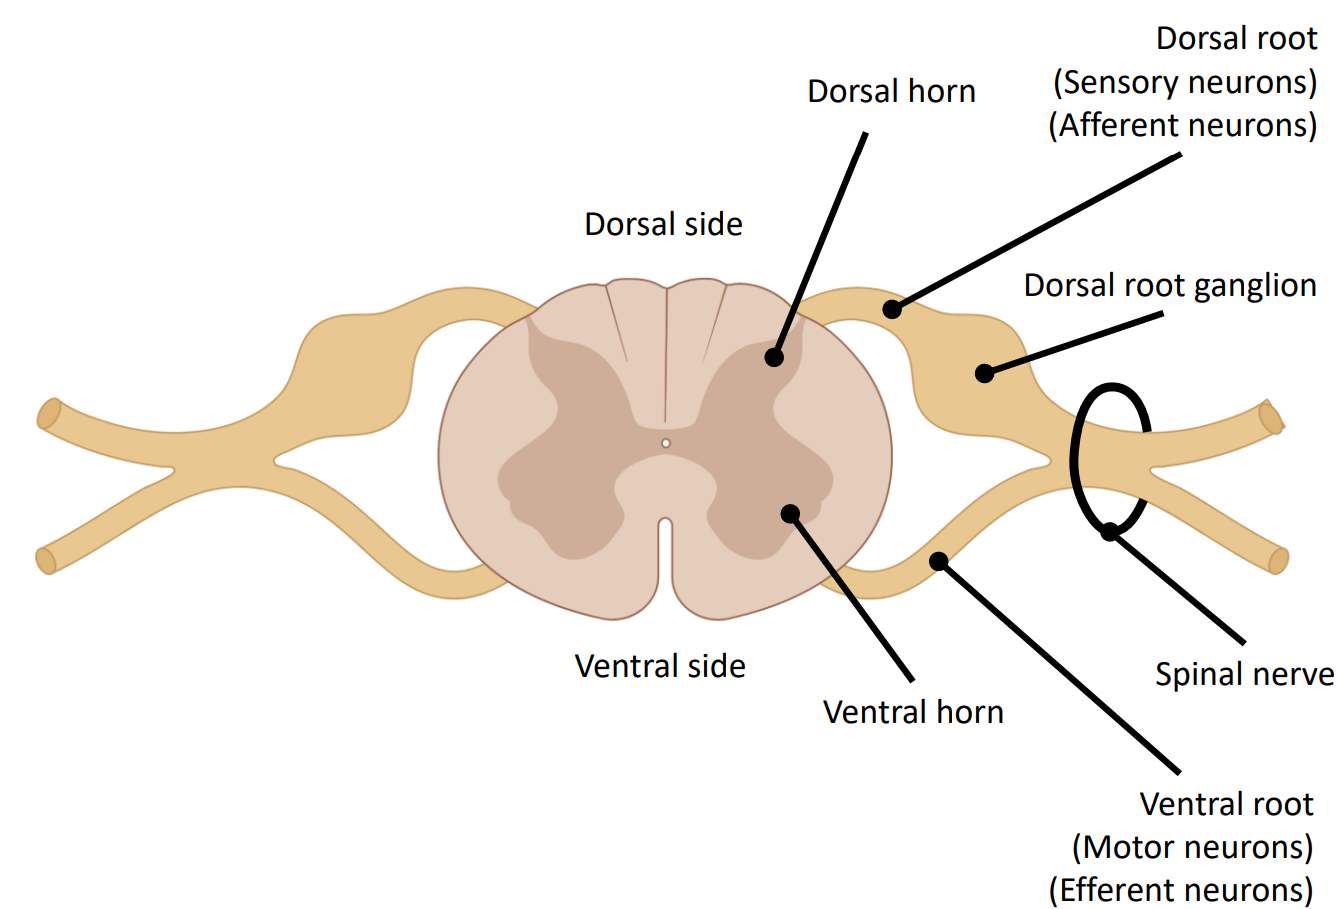
\includegraphics[width=0.65\linewidth]{Pictures/Screenshot 2024-03-06 201615.png}
\end{center}
\begin{exercise}
    How do neurons enter and exit the spinal column and how they travel to and from the brain?
    \begin{enumerate}
        \item \textcolor{blue}{Neurons (specifically axons) get bundled into fascicles to become a nerve} 
        \item \textcolor{blue}{Spinal cord consists of grey matter (located in center, shaped like butterfly, contains neuron cell bodies) and white matter (contains myelinated axons that carry signals)}
        \item \textcolor{blue}{Neurons connect to spinal cord through either dorsal (posterior, sensory) or ventral (anterior, motor) roots}
        \item \textcolor{blue}{\textbf{Ganglia:} structure of oval shape containing neuron cell bodies, glial tissue (support and function), and connective tissue}
        \item \textcolor{blue}{Sensory neurons enter spinal cord through dorsal roots, cell bodies are located in dorsal root ganglia}
        \item \textcolor{blue}{Motor neurons have cell bodies in grey matter of spinal cord and axons go out via ventral roots to innervate muscles}
    \end{enumerate}
\end{exercise}
\begin{exercise}
    What is the difference between efferent and afferent nerve fibres (axon)?

    \textcolor{blue}{They are the same: Sensory Afferent (In); Motor Efferent (Out)}
\end{exercise}
\begin{exercise}
    What components do reflex arcs have?
    \textcolor{blue}{
    \begin{itemize}
        \item receptor
        \item sennsory neuron (afferent pathway)
        \item integration centre
        \item motor neuron (efferent pathway)
        \item effector
    \end{itemize}
    }
\end{exercise}

\section{Peripheral Nervous System}
\textbf{Mechanically-gated (mechanosensitive) ion channels}
\begin{center}
    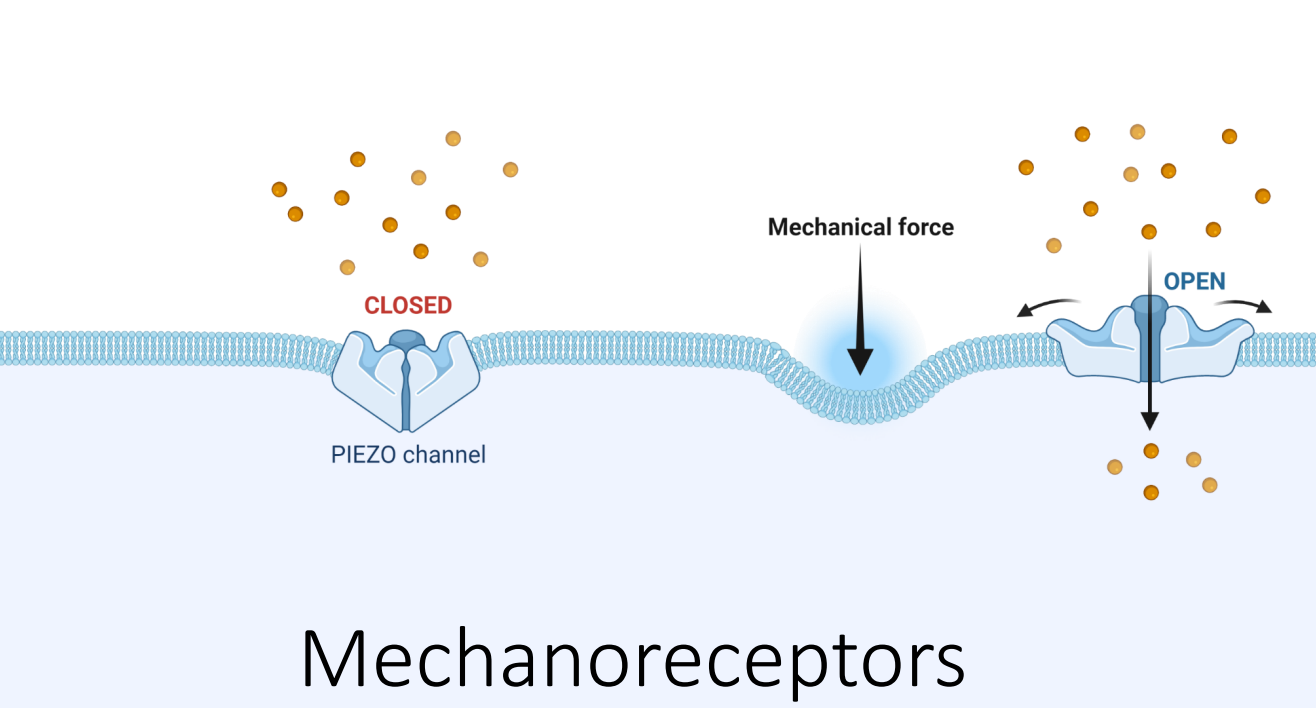
\includegraphics[width=0.65\linewidth]{Pictures/Screenshot 2024-03-06 192802.png}
\end{center}
\textbf{Receptor potential to action potential:} Receptors may be a part of the afferent neuron (e.g. touch, pain, itch, tickle, pressure, smell) or there may be whole receptor cells that interface with the afferent neuron (e.g. vision, hearing, equilibrium)
\begin{center}
    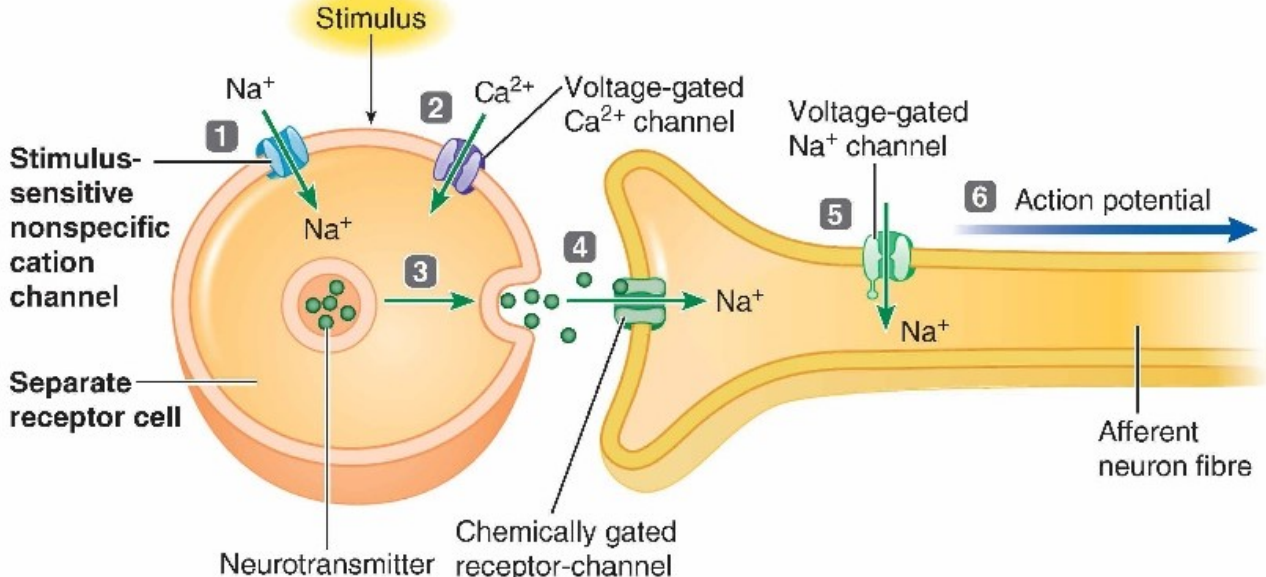
\includegraphics[width=0.65\linewidth]{Pictures/Screenshot 2024-03-06 193004.png}
\end{center}
\textbf{MILD}
\begin{itemize}
    \item Modality
    \item Intensity
    \item Location
    \item Duration
\end{itemize}

\subsection{Modelity}
Modelity: Type or nature (e.g. touch, pain, sound) is determined by specific receptor activated by stimulus.

\textbf{Sensors by modelity}
\begin{itemize}
    \item mechanoreceptors
    \begin{itemize}
        \item somatosensory: touch
        \item baroreceptors: blood pressure
        \item proprioceptors: position and movement
        \item osmoreceptors: osmotic pressure
    \end{itemize}
    \item thermoreceptors
    \item nociceptors: pain
    \item photoreceptors: light
    \item chemoreceptors: chemical composition of blood
\end{itemize}
\begin{descriptions}
    \item[Free nerve endings:] Simplest receptors are free nerve endings (dendrites) and have no special structure
    \item[Encapsulated nerve ending:] Encapsulated nerve endings are covered by nerve tissue (e.g. insulated) which makes them more selective. Capable of detecting pain, pressure, temperature
    \item[Sensory cell:] Unique sensory (receptor) cells also exist. These cells interface with the sensory neuron. Example are photoreceptors (rod or cone) 
    \item[Peripheral processes:] Closest to structure we’ve studied so far. Receptors in dendrites attached to cell body. Olfactory receptor is an example 
\end{descriptions}
\begin{center}
    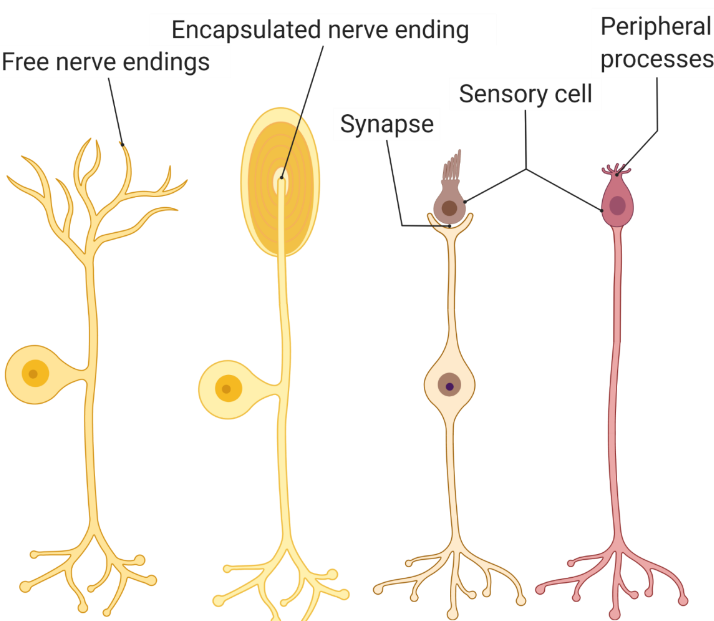
\includegraphics[width=0.65\linewidth]{Pictures/Screenshot 2024-03-06 193746.png}
\end{center}

\subsection{Intensity, Location, Duration}
\subsubsection{Intensity}
\textbf{Frequency coding:} The larger the receptor potential, the greater the frequency of action potentials
\begin{center}
    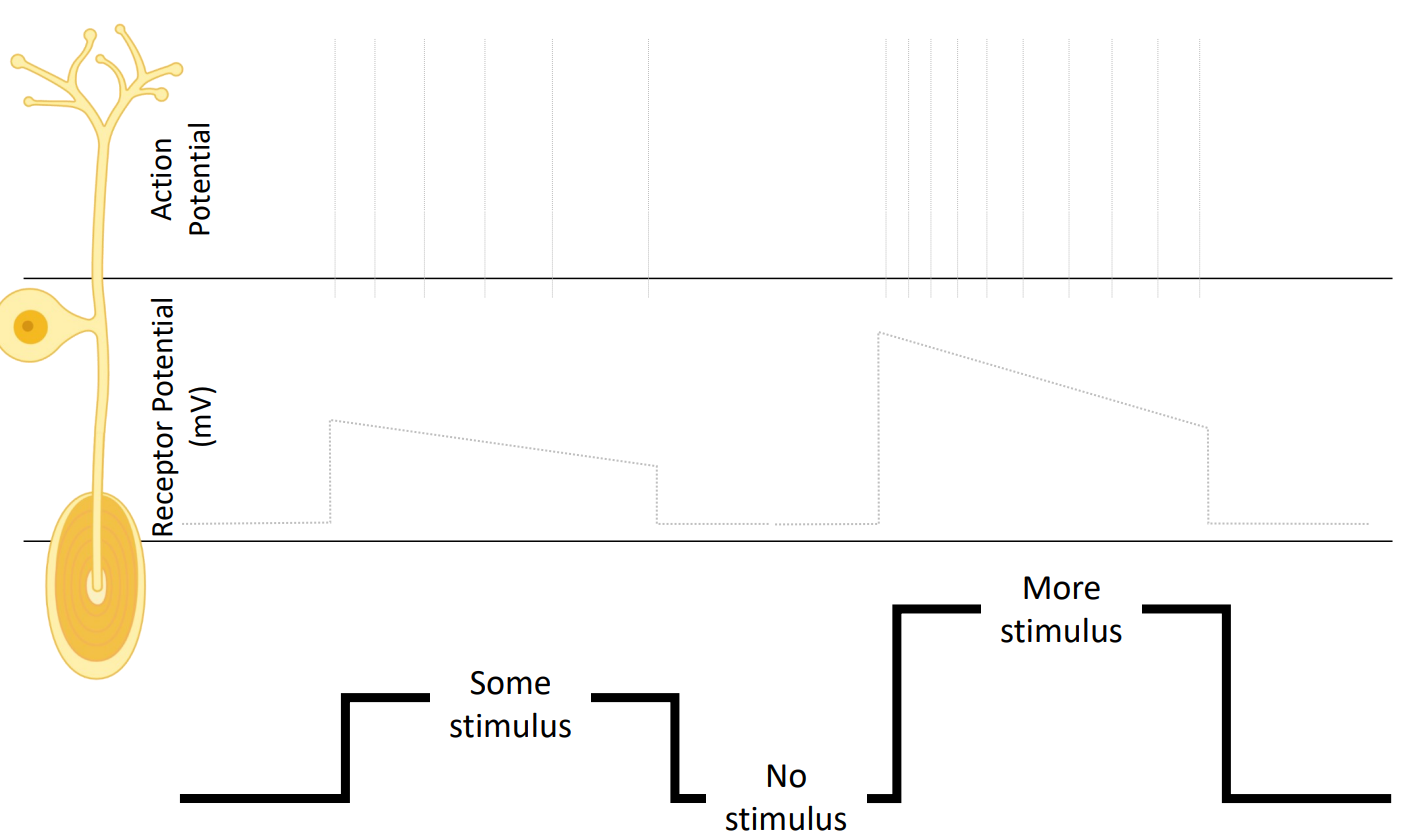
\includegraphics[width=0.65\linewidth]{Pictures/Screenshot 2024-03-06 194015.png}
\end{center}

\subsubsection{Location}
\textbf{Receptive field}
\begin{itemize}
    \item The more densely receptors are spaced, the smaller area of skin each monitors
    \item Smaller receptive field equals greater acuity
    \item 17,000 on hand vs a few on elbow
\end{itemize}
\textbf{Lateral inhibition}
\begin{itemize}
    \item Process in nervous system to enhance precision of sensory perception
    \item Excited neuron (center) reduces activity of neighbours
    \item Amplifies excited neuron by contrast
\end{itemize}


\subsubsection{Duration}
\textbf{Adaptation to a sustained stimulus}
\begin{itemize}
    \item \textbf{Phasic receptors:} 
    \begin{itemize}
        \item phasic receptors adapt rapidly to stimulus
        \item initial response occurs, but then diminishes (i.e. few APs generated)
    \end{itemize}
    \item \textbf{Tonic receptors:}
    \begin{itemize}
        \item tonic receptors adapt slowly to stimulus
        \item continue to generate APs over duration of stimulus
    \end{itemize}
\end{itemize}

\textbf{Types of Somatic Receptors in the cutaneous/subcutaneous layer}
\begin{itemize}
    \item somatic receptors are a part of the somatosensory system
    \item \textbf{somatiosensory system:} receives and processes sensory information
    \item \textbf{somatic nervous system:} part of PNS that controls voluntary movement
\end{itemize}

\subsection{Neuromuscular Junction}
\textbf{Motor end-plate and innervation of skeletal muscle}
\begin{itemize}
    \item motor neurons interfaces to multiple muscle fibers
    \item motor unit: neuron and all fibers it innervates
    \item AP in motor neuron triggers acetycholine release (neuraltransmitter)
    \item triggers muscle fiber sliding (contract/relax)
\end{itemize}

\section{Autonomic Nervous System}
\textbf{Somatic motor system:} typically, a single motor neuron can run from the spinal cord to innervate a muscle

\textbf{Autonomic motor system:} 
\begin{itemize}
    \item ANS typically has a chain of two neurons: first has cell body in CNS (e.g. spinal cord), second has cell body close to spinal cord or organ
    \item specifically, preganglionic neuron has cell body in CNS, postganglionic neuron has cell body in ganglion
    \item \textbf{Ganglion (ANS):} collection of nerve cell bodies that acts as a relay point where preganglionic neurons synapse with postganglionic neurons. They also contain connective tissue (structure/protect), (nutrient supply), other nerve fibers
\end{itemize}

\subsection{Autonomic Nervous System Structure}
\textbf{Sympathetic ganglion chain}
\begin{itemize}
    \item series of interconnected gangglia
    \item ganglis connected by interganglionic fibres
    \item runs paraller to spinal cord
    \item extends from base of skull to coccyx
\end{itemize}

\textbf{Central neurons may...}
\begin{itemize}
    \item synapse with ganglion at same level 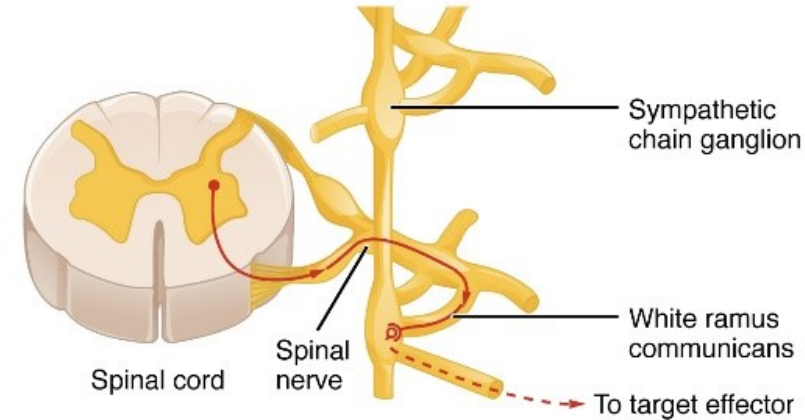
\includegraphics[width=120pt]{Pictures/Screenshot 2024-03-06 202747.png}
    \item synapse with a more superior/inferior ganglion 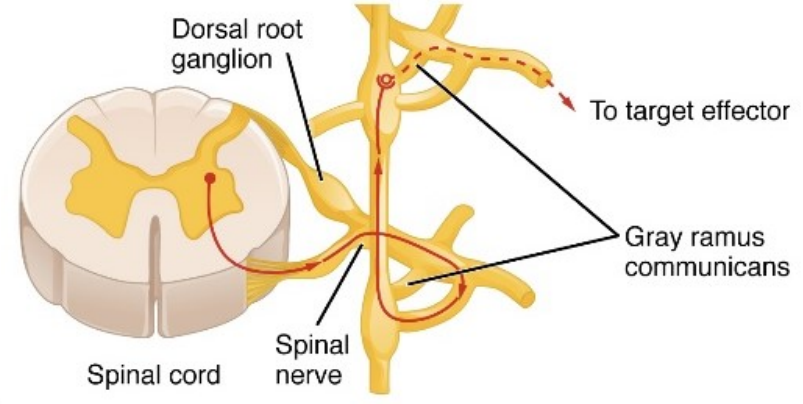
\includegraphics[width=120pt]{Pictures/Screenshot 2024-03-06 202752.png}
    \item synapse with ganglion outside of the chain (i.e. bypasses sympathetic chain) 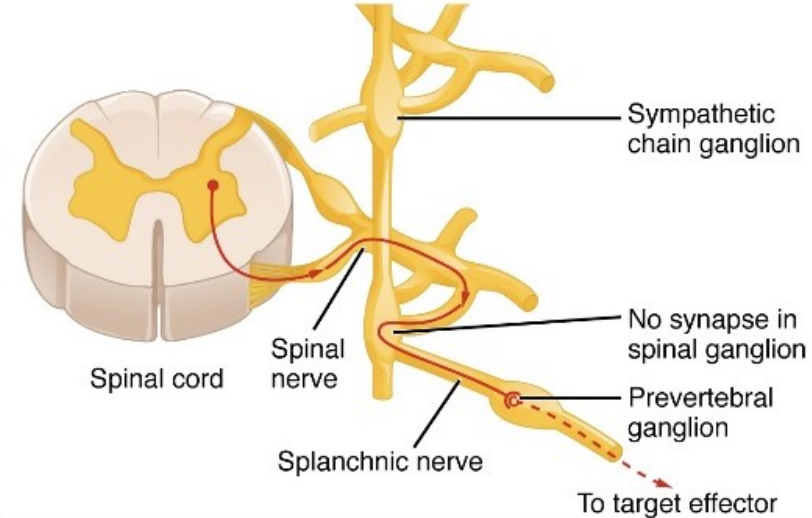
\includegraphics[width=120pt]{Pictures/Screenshot 2024-03-06 202757.png}
\end{itemize}

\textbf{There are only sympathetic nerves to:}
\begin{itemize}
    \item adrenal glands
    \item sweat glands
    \item arterioles (vasoconstriction)
    \item note: sympathetic pathways usually have short preganglionic neuron and long postganglionic neuron
\end{itemize}

\subsubsection{Therapeutic solutions}
\textbf{Baroflex activation therapy}
\begin{itemize}
    \item implantable pulse generator
    \item delivers continuous electrical stimulation to carotid baroreceptors
    \item increases inhibition of tonically active outflow to peripheral vasculature
    \item results in vasodilation and decrease peripheral vascular resistance
\end{itemize}

\textbf{Vagus nerve stimulation}
\begin{itemize}
    \item electrical stimulate left vagus nerve to implant signals in the brain
    \item particularly stimulates to treat seizures, depression, aid in stroke recovery
\end{itemize}

\textbf{There are only parasympathetic nerves from:}
\begin{itemize}
    \item cranial
    \item sacral
    \item note: parasympathetic pathways usually have long preganglionic neuron and short postganglionic neuron
\end{itemize}

\textbf{3 major axon groups}
\begin{enumerate}
    \item \begin{itemize}
        \item sensory neurons
        \item somatic motor neurons
        \item 70-120 m/s
    \end{itemize}
    \item \begin{itemize}
        \item preganglionic autonomic neurons
        \item 3-15 m/s
    \end{itemize}
    \item \begin{itemize}
        \item postganglionic autonomic neurons
        \item AP from toe to spinal cord $\approx$ 4s (0.3-2 m/s)
    \end{itemize}
\end{enumerate}

\subsection{Cholinergic and Adrenergic Receptors}
\textbf{Neuroeffector junction (NEJ)}
\begin{itemize}
    \item specialize synapse between neuron and target effector (non-neuron)
    \item effector may be smooth muscle (e.g. heart, intestine or gland)
    \item neuron elicits physiological response (e.g. muscle contraction or gland secretion)
    \item note: in somatic system we say neuromuscular junction, in autonomic system we say neuroeffector junstion
\end{itemize}

\textbf{Postganglionic neurotransmitter release}
\begin{itemize}
    \item sympathetic
    \begin{itemize}
        \item norepinephrine
        \item epinephrine
    \end{itemize}
    \item parasympathetic
    \begin{itemize}
        \item acetylcholine
    \end{itemize}
\end{itemize}

\begin{center}
    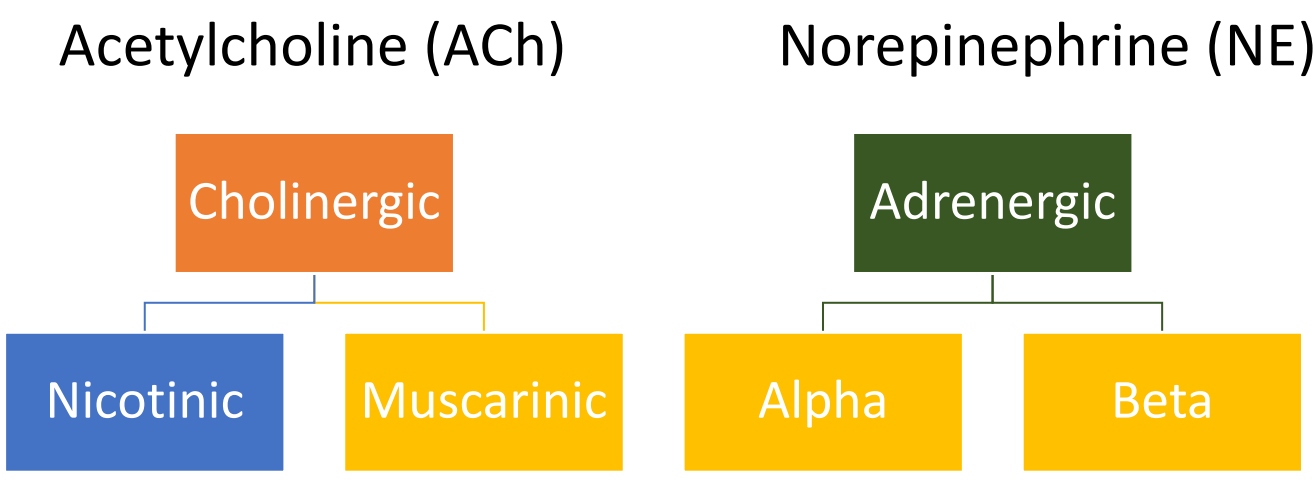
\includegraphics[width=0.65\linewidth]{Pictures/Screenshot 2024-03-06 204921.png}
\end{center}

\subsubsection{Acetylcholine (ACh)}

\textbf{Nicotinic}
\begin{itemize}
    \item ionotropic receptors
    \item allow positive ions across cell membranes 
    \item skeletal muscle contraction, cognitive function, arousal
\end{itemize}

\textbf{Muscarinic}
\begin{itemize}
    \item metabotropic receptors
    \item produce more prolonged/diverse effects
    \item regulate gland secretion, smooth muscle contraction, heartrate
\end{itemize}

\subsubsection{Norepinephrine (NE)}

\textbf{Alpha}
\begin{itemize}
    \item found in smooth muscle and presynaptic neuron terminals
    \item control vasoconstriction (blood pressure)
    \item mediate smooth musclew contraction (bladder)
    \item may inhibit NE release (i.e. inhibit sympathetic neuron activity)
\end{itemize}

\textbf{Beta}
\begin{itemize}
    \item found in heart, kidney, airways, arteioles, skeletal muscle, fatty tissues
    \item can increase heart rate, impact blood pressure via kidneys, relax smooth muscle, break down fats
\end{itemize}

\begin{center}
    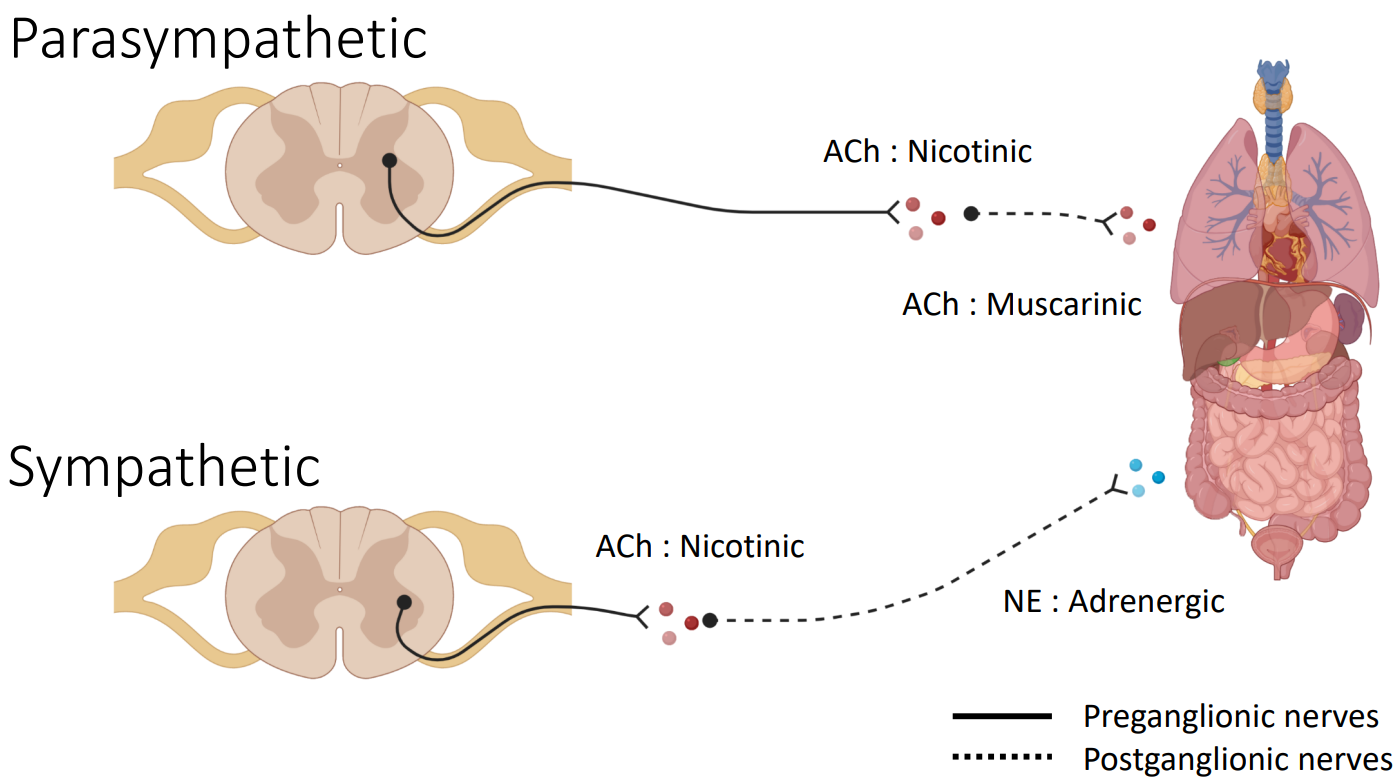
\includegraphics[width=0.65\linewidth]{Pictures/Screenshot 2024-03-06 205513.png}
\end{center}

\begin{exercise}
    \begin{center}
    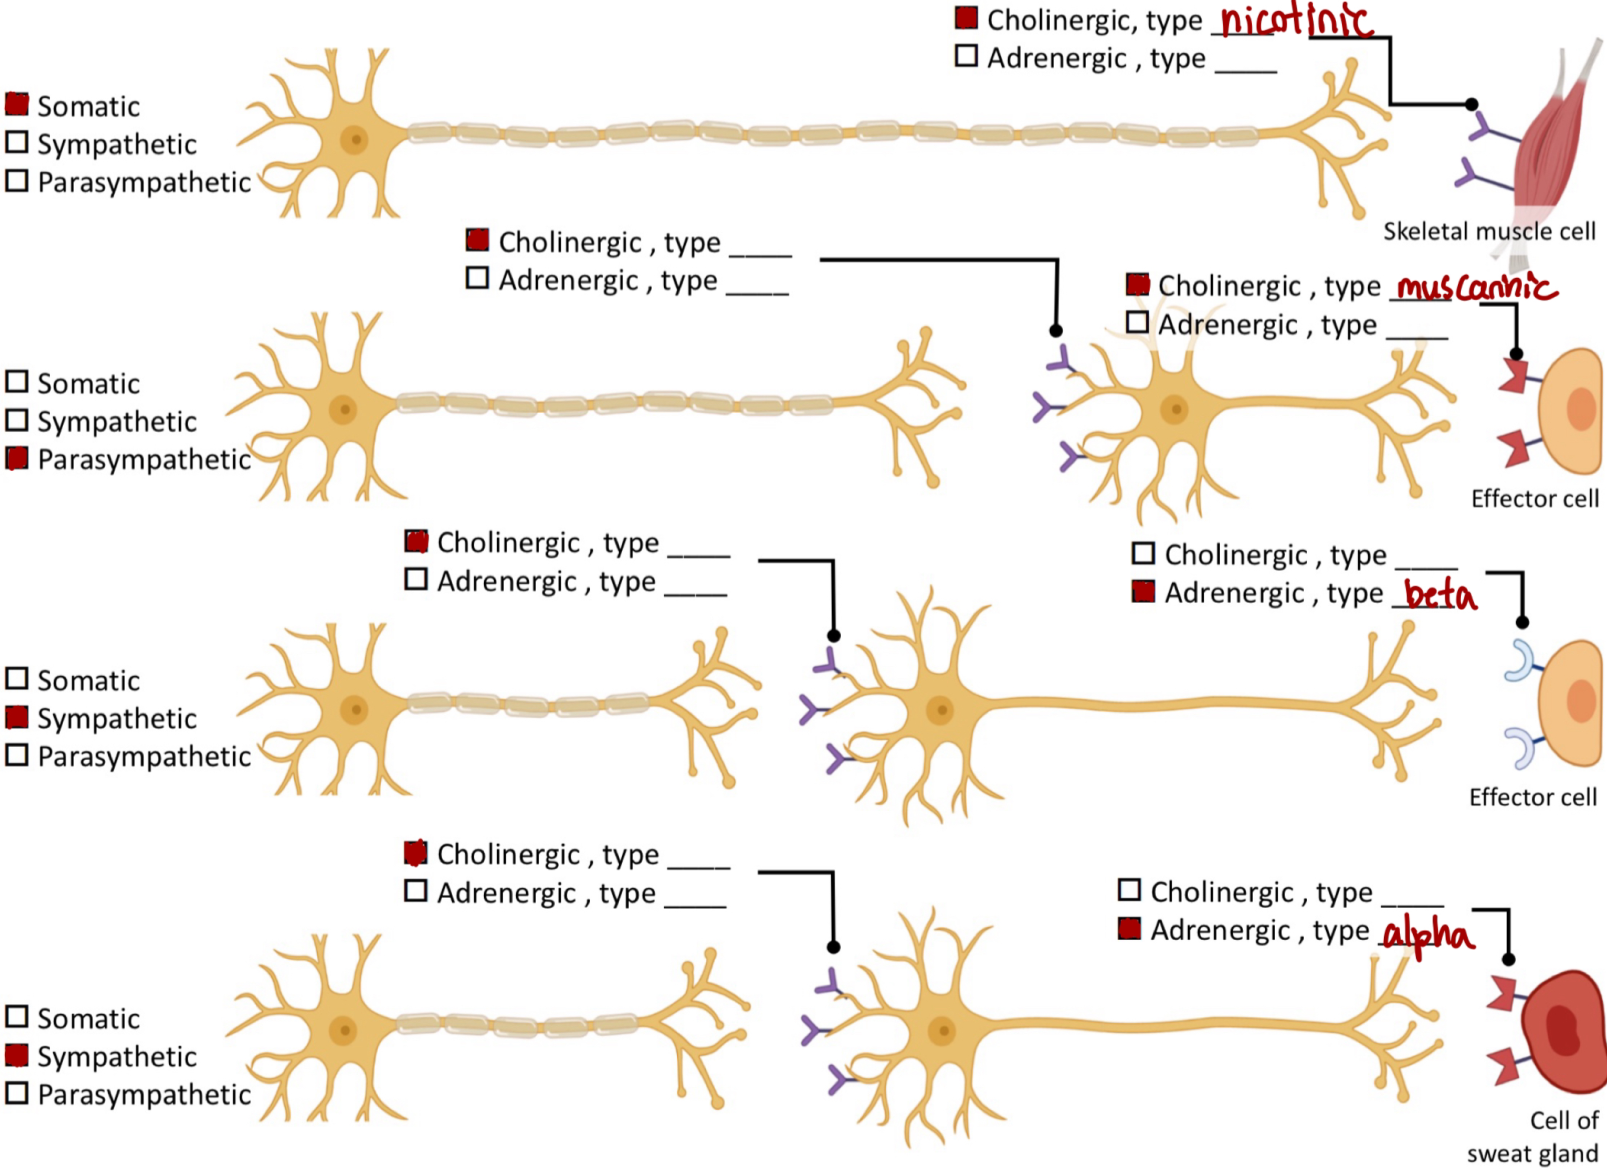
\includegraphics[width=0.95\linewidth]{Pictures/Screenshot 2024-04-03 230126.png}
\end{center}
\end{exercise}

\chapter{Muscles}
\section{Skeletal Muscles}
\subsection{Building Blocks of the Musculoskeletal System}
\textbf{Human Skeleton}
\begin{itemize}
    \item Protects
    \item Provides structure
    \item Creates joints (between bones)
    \item Allows for articulation but does not actuate
\end{itemize}

\textbf{Types of Contractions}
\begin{figure}[h!]
    \centering
    \begin{subfigure}{0.45\textwidth}
        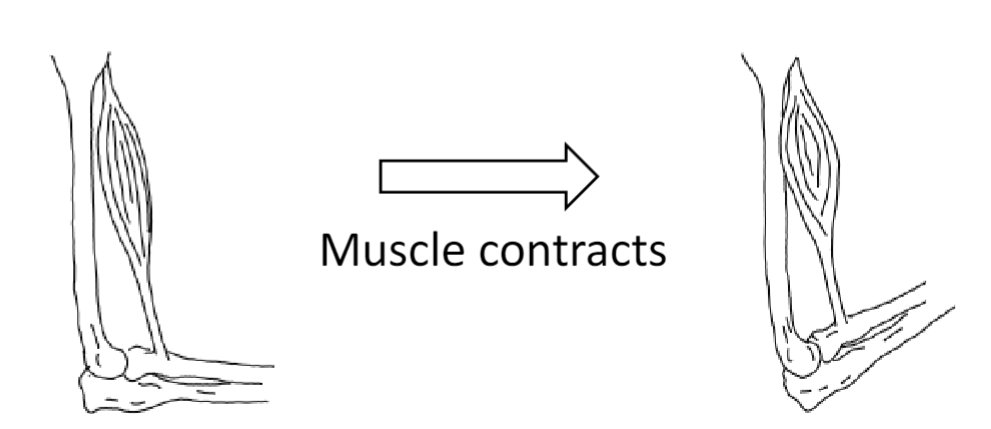
\includegraphics[width=\textwidth]{Pictures/Screenshot 2024-04-03 000405.png}
        \caption{Concentric: muscle shortens
as contracts (e.g. lifting
action)}
    \end{subfigure}
    \hfill
    \begin{subfigure}{0.45\textwidth}
        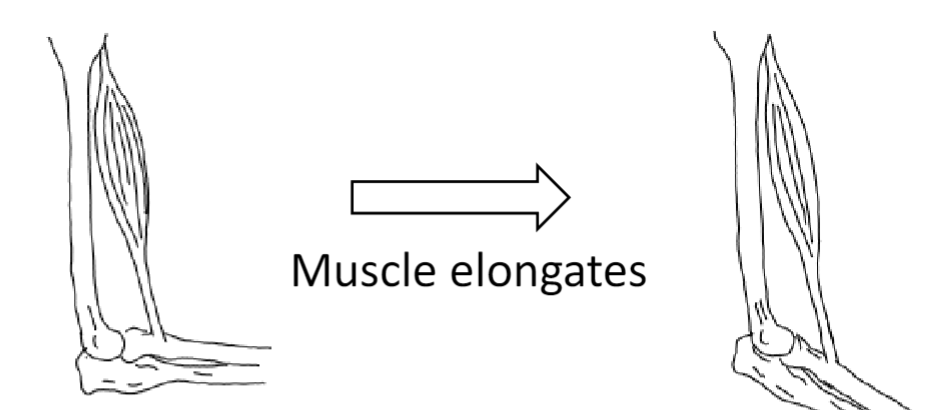
\includegraphics[width=\textwidth]{Pictures/Screenshot 2024-04-03 000414.png}
        \caption{Concentric: muscle lengthens
under tension (e.g. lowering
action)}
    \end{subfigure}
    \begin{subfigure}{0.45\textwidth}
        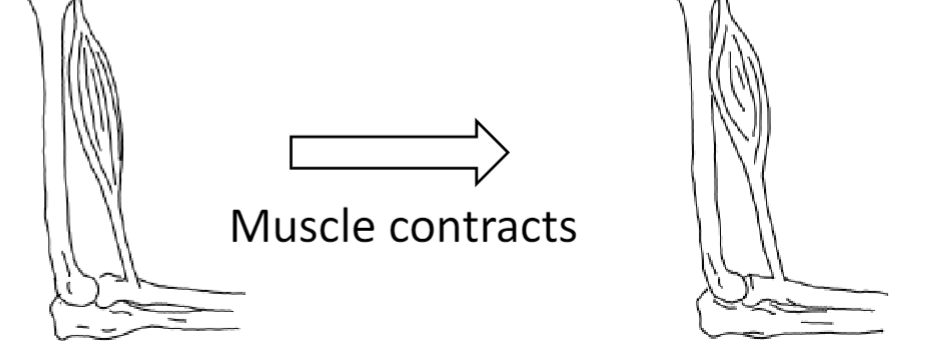
\includegraphics[width=\textwidth]{Pictures/Screenshot 2024-04-03 000424.png}
        \caption{Concentric: muscle generates
force without changing length
(e.g. hold weight without
moving)}
    \end{subfigure}
    \caption{}
\end{figure}


\textbf{Joints, Cartilage, Ligaments, Tendons}
\begin{descriptions}
    \item[Joint: ]connection between two bones
    \item[Cartilage: ]ECM (collagenous connective tissue, absorbs shock, reduces friction (passive)
    \item[Tendon: ]elastin \& collagenous
connective tissue, connects muscle
to bone, supports actuation
(passive) 
    \item[Ligament: ]mostly collagenous
connective tissue, connects bone
to bone, supports actuation,
reinforces skeletal structure
(passive) 
\end{descriptions}

\subsection{Skeletal Muscle Structure}
\textbf{Types of Muscle}
\begin{descriptions}
    \item[Skeletal: ]voluntary, striated,
attach to bones, control
conscious movement
    \item[Smooth: ]involuntary, non-
striated, found in hollow organs
(stomach, intestines, blood
vessels) 
    \item[Cardiac: ]involuntary, striated,
found in heart only
\end{descriptions}

\textbf{Striated Muscle}
\begin{itemize}
    \item Alternating light \& dark bands under microscopy
    \begin{itemize}
        \item Skeletal \& cardiac muscle highly organized
        \item Contractile protein (actin \& myosin) organization in
muscle fibers creates striation
        \item Organization allows for precise control \& powerful
contractions
    \end{itemize}
    \item Smooth muscle has less orderly arrangement and
so no striation
\end{itemize}

\textbf{Components}
\begin{descriptions}
    \item[Epimysium: ]Sheath of fibrous, elastic
tissue surrounding muscle
    \item[Fascicle: ]Muscle sub-unit, bundle of muscle fibres
(muscle cells 
    \item[Perimysium: ]Sheath of connective
tissue surrounding bundle
of muscle fibres (fascicle)
    \item[Muscle fiber: ]Long single cylindrical muscle cell, contractile cell, multinucleated (skeletal
cells only) due to large
amount of protein \&
enzymes required, nuclei are close to
sarcolemma (cell
membrane)
    \item[Endomysium: ]Wispy connective tissue
sheath surrounding
each muscle fibre
\end{descriptions}
\begin{center}
    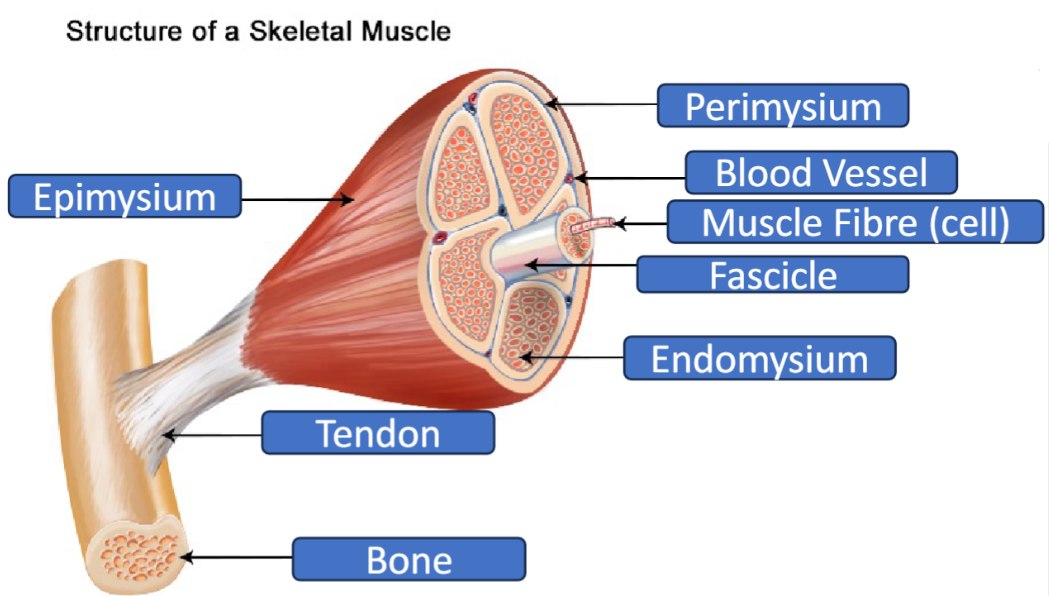
\includegraphics[width=0.65\linewidth]{Pictures/Screenshot 2024-04-03 002531.png}
\end{center}

\textbf{Key Points}
\begin{itemize}
    \item Fascicle contains around 20 to 60 fibers
    \item One nerve may innervate fibers across >100 fascicles
    \item Muscle fibre is the cell
    \item Sarcolemma is cell membrane
    \item \textbf{\textit{Myofibril}}
    \begin{itemize}
        \item basic rod-like organelle of a muscle fiber
        \item made of sarcomeres
        \item sarcomeres made of myofilaments (actin \& myosin)
    \end{itemize}
\end{itemize}
\begin{center}
    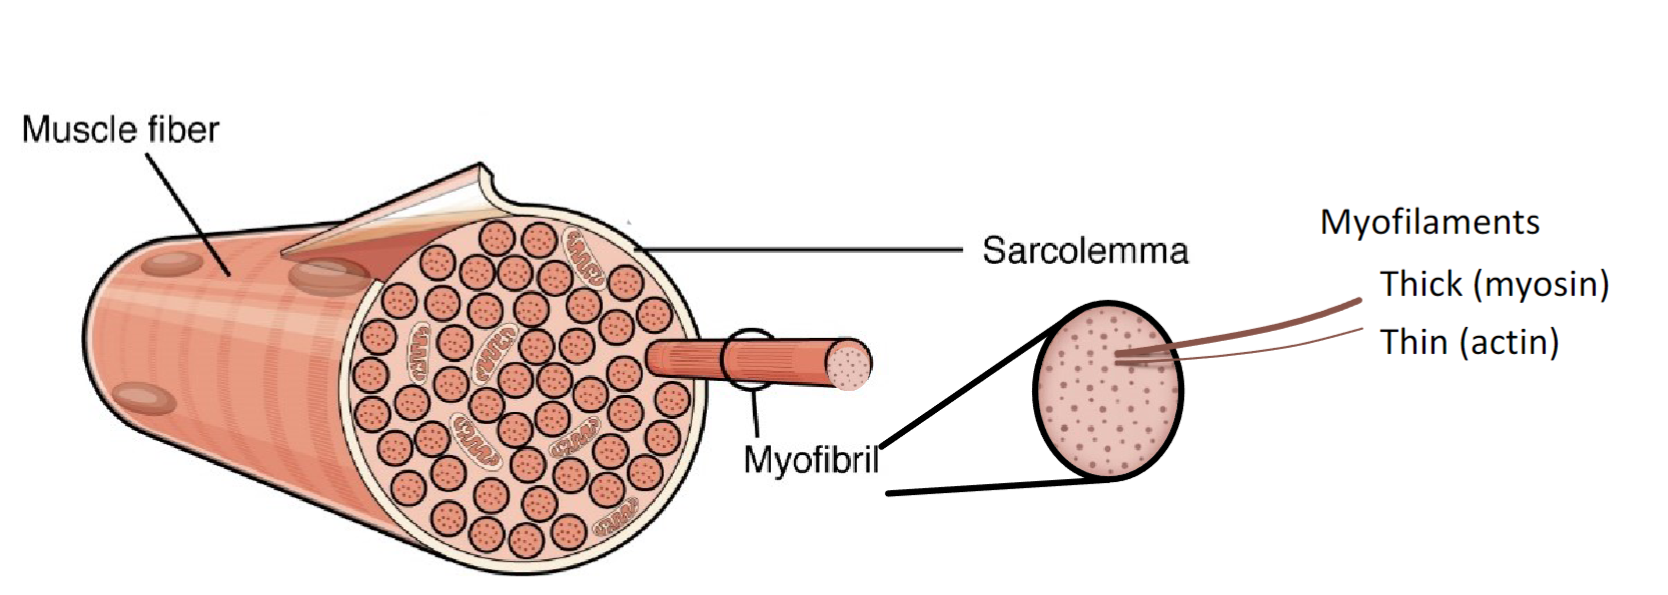
\includegraphics[width=0.65\linewidth]{Pictures/Screenshot 2024-04-03 005053.png}
\end{center}
\textbf{Overview of Structure}
\begin{center}
    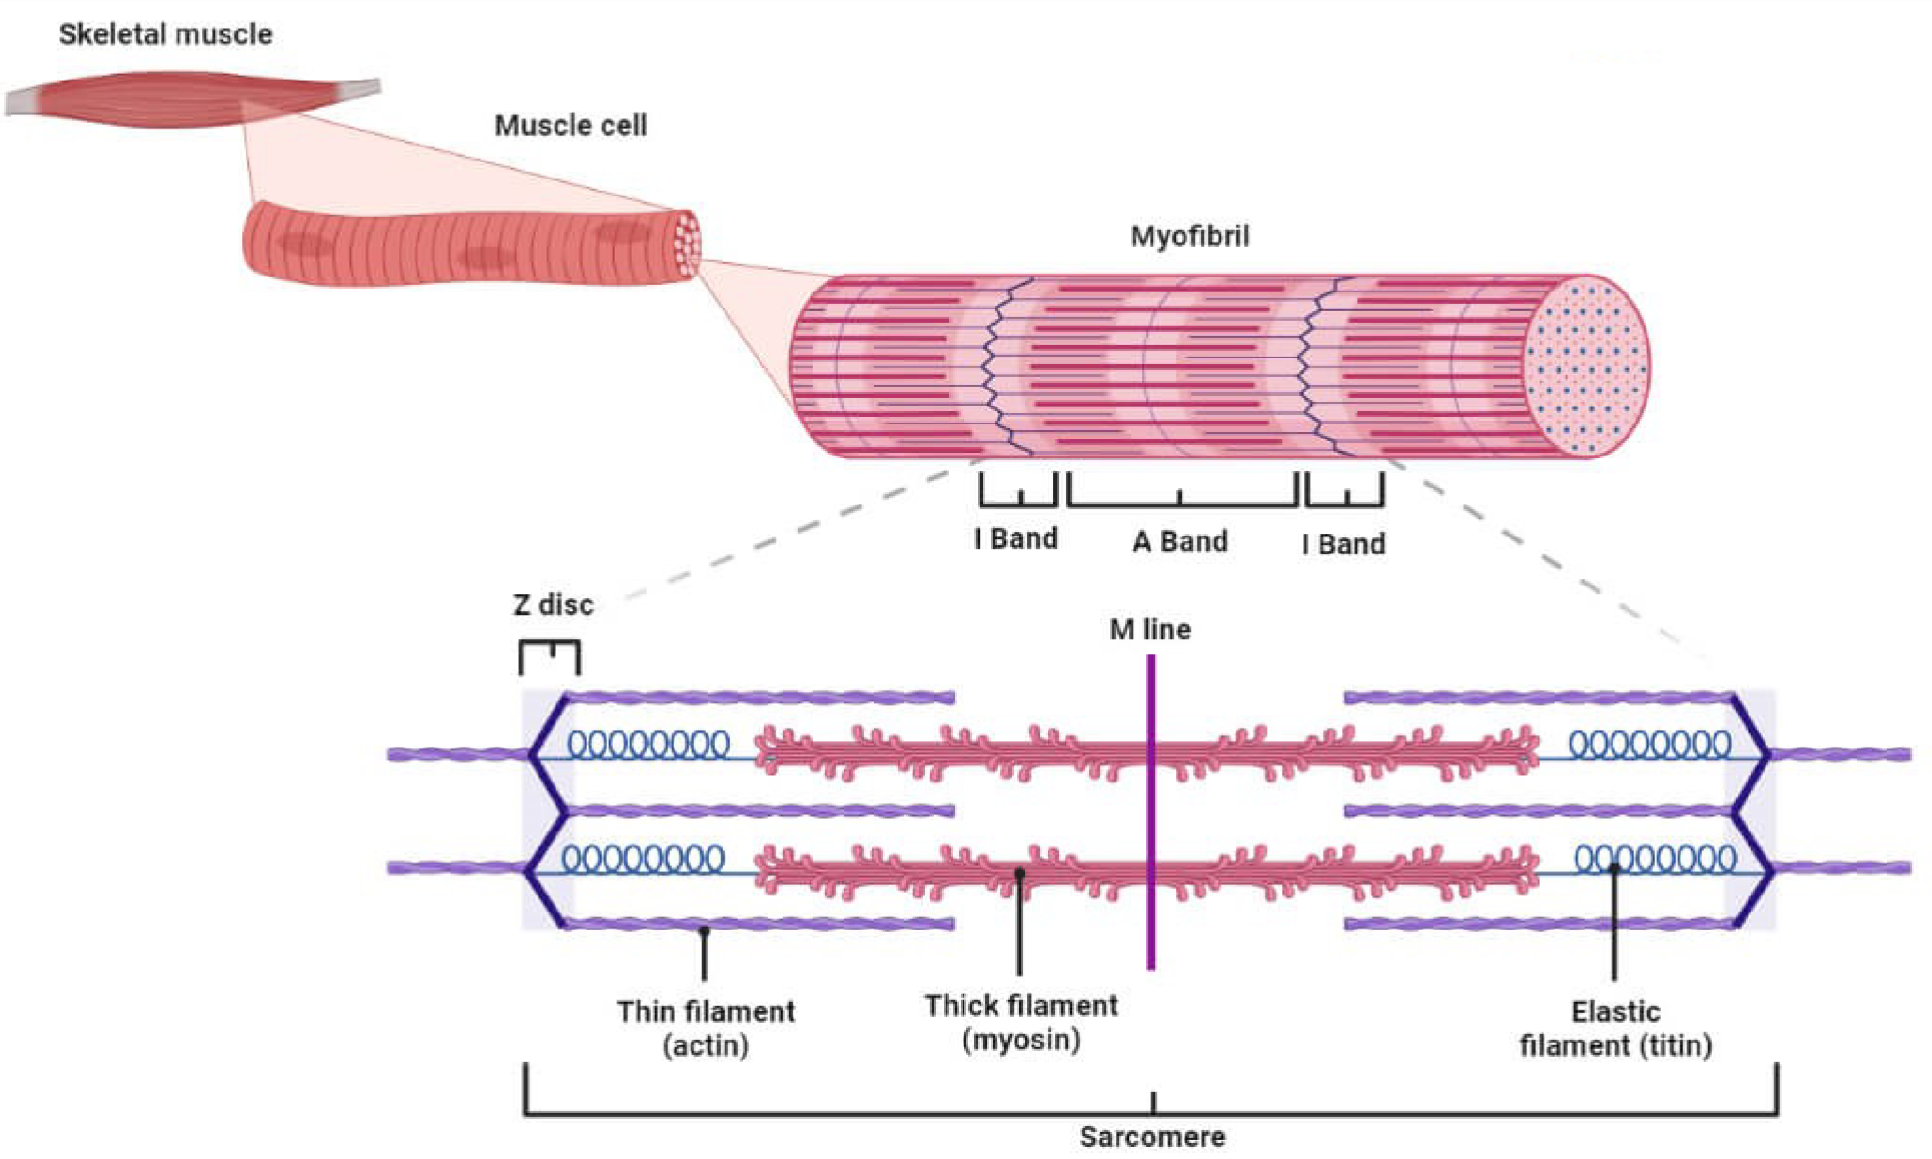
\includegraphics[width=0.65\linewidth]{Pictures/Screenshot 2024-04-03 005340.png}
\end{center}
\textbf{Sarcomere}
\begin{center}
    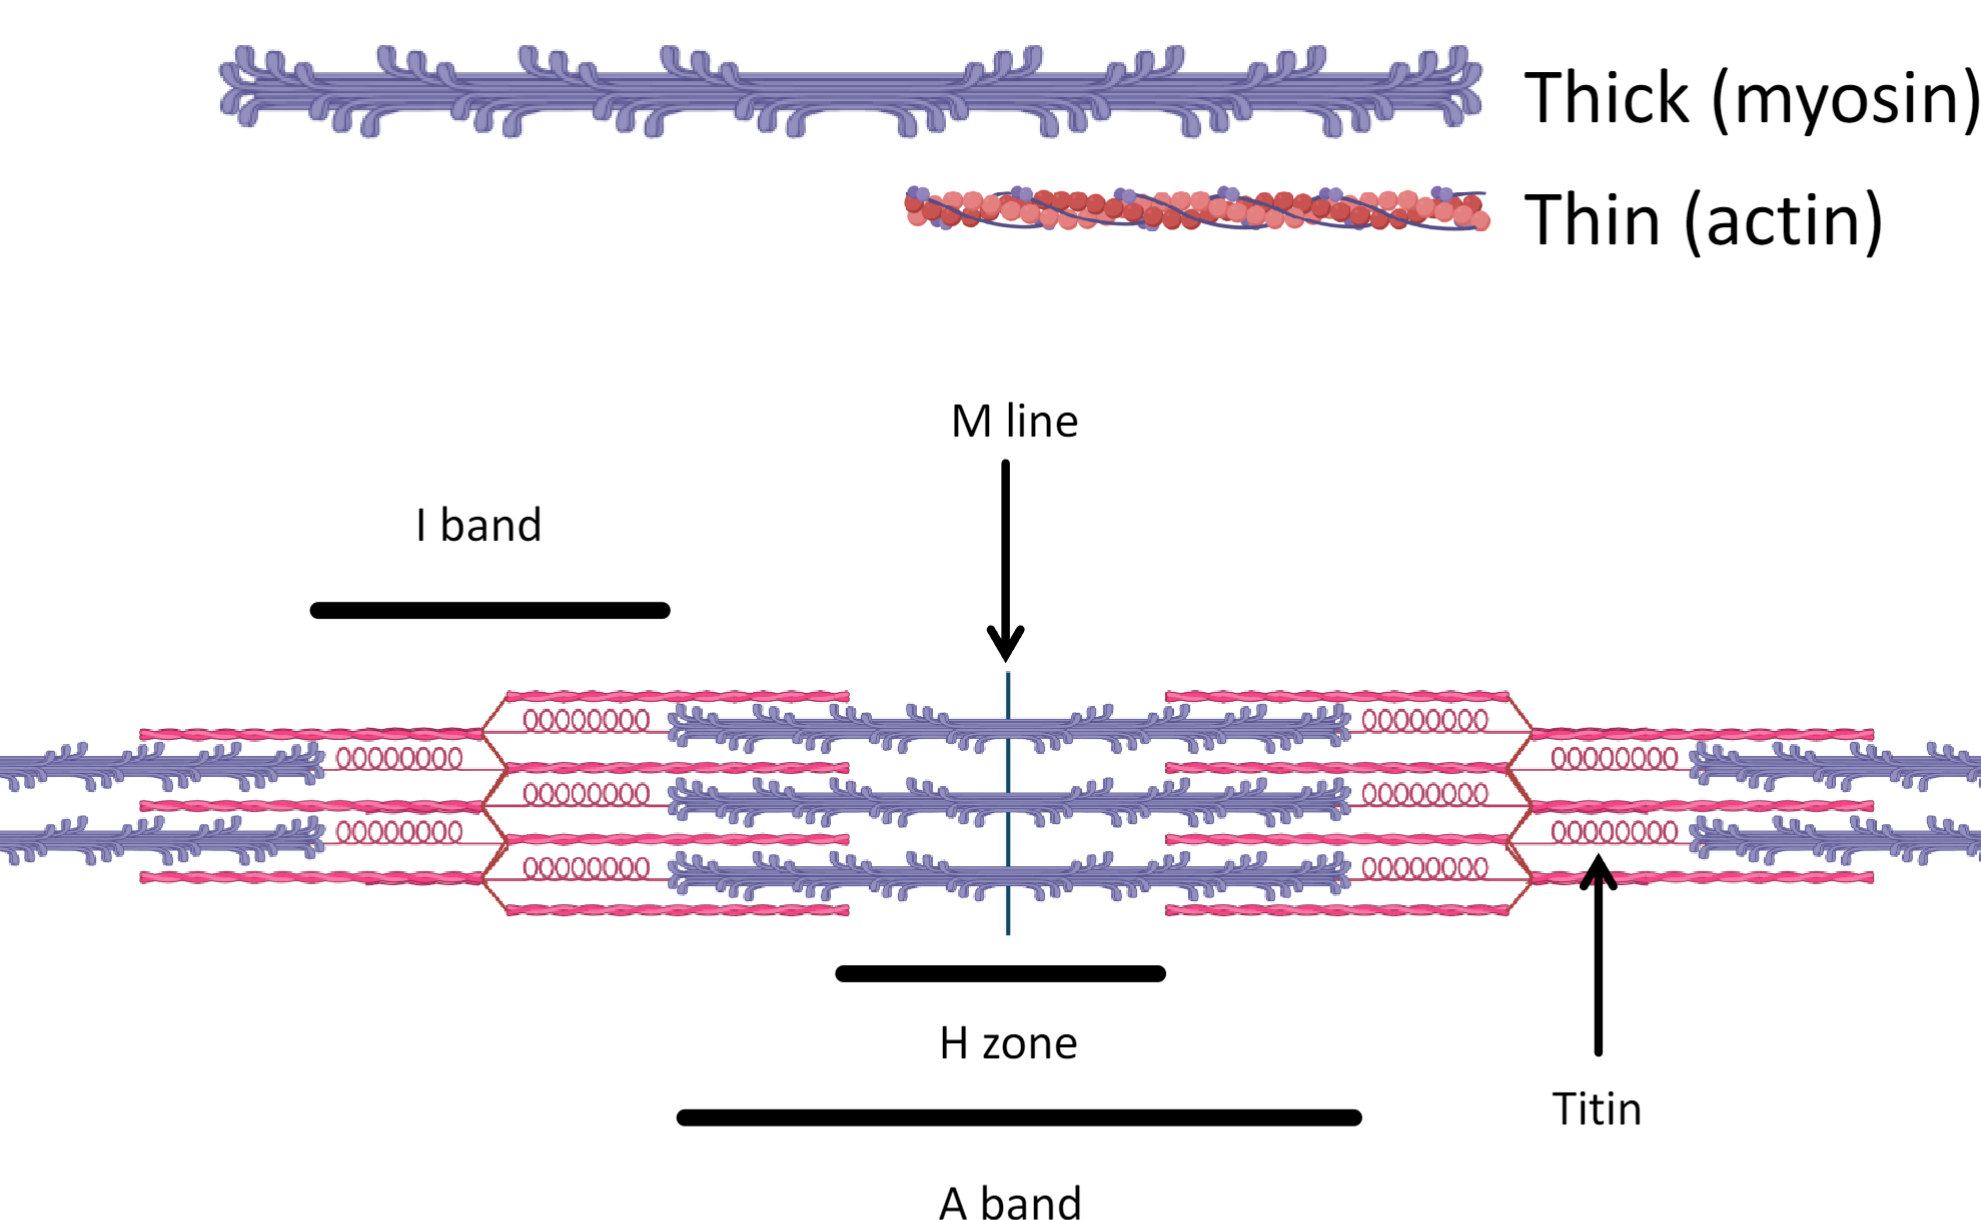
\includegraphics[width=0.65\linewidth]{Pictures/Screenshot 2024-04-03 005431.png}
\end{center}
\begin{descriptions}
    \item[M line: ]Attachment point that aligns myosin (thick)
filaments in sarcomere 
    \item[Z line: ]Marks the boundaries of each sarcomere 
    \item[H zone: ]Region around M line where only myosin is
present (no actin overlap)
    \item[I band: ]Region containing only actin filaments (no
myosin overlap)
\end{descriptions}

\subsection{Neuromuscular Junction}
\begin{remark}
    Motor neurons innervate skeletal muscle cells
\end{remark}
\begin{center}
    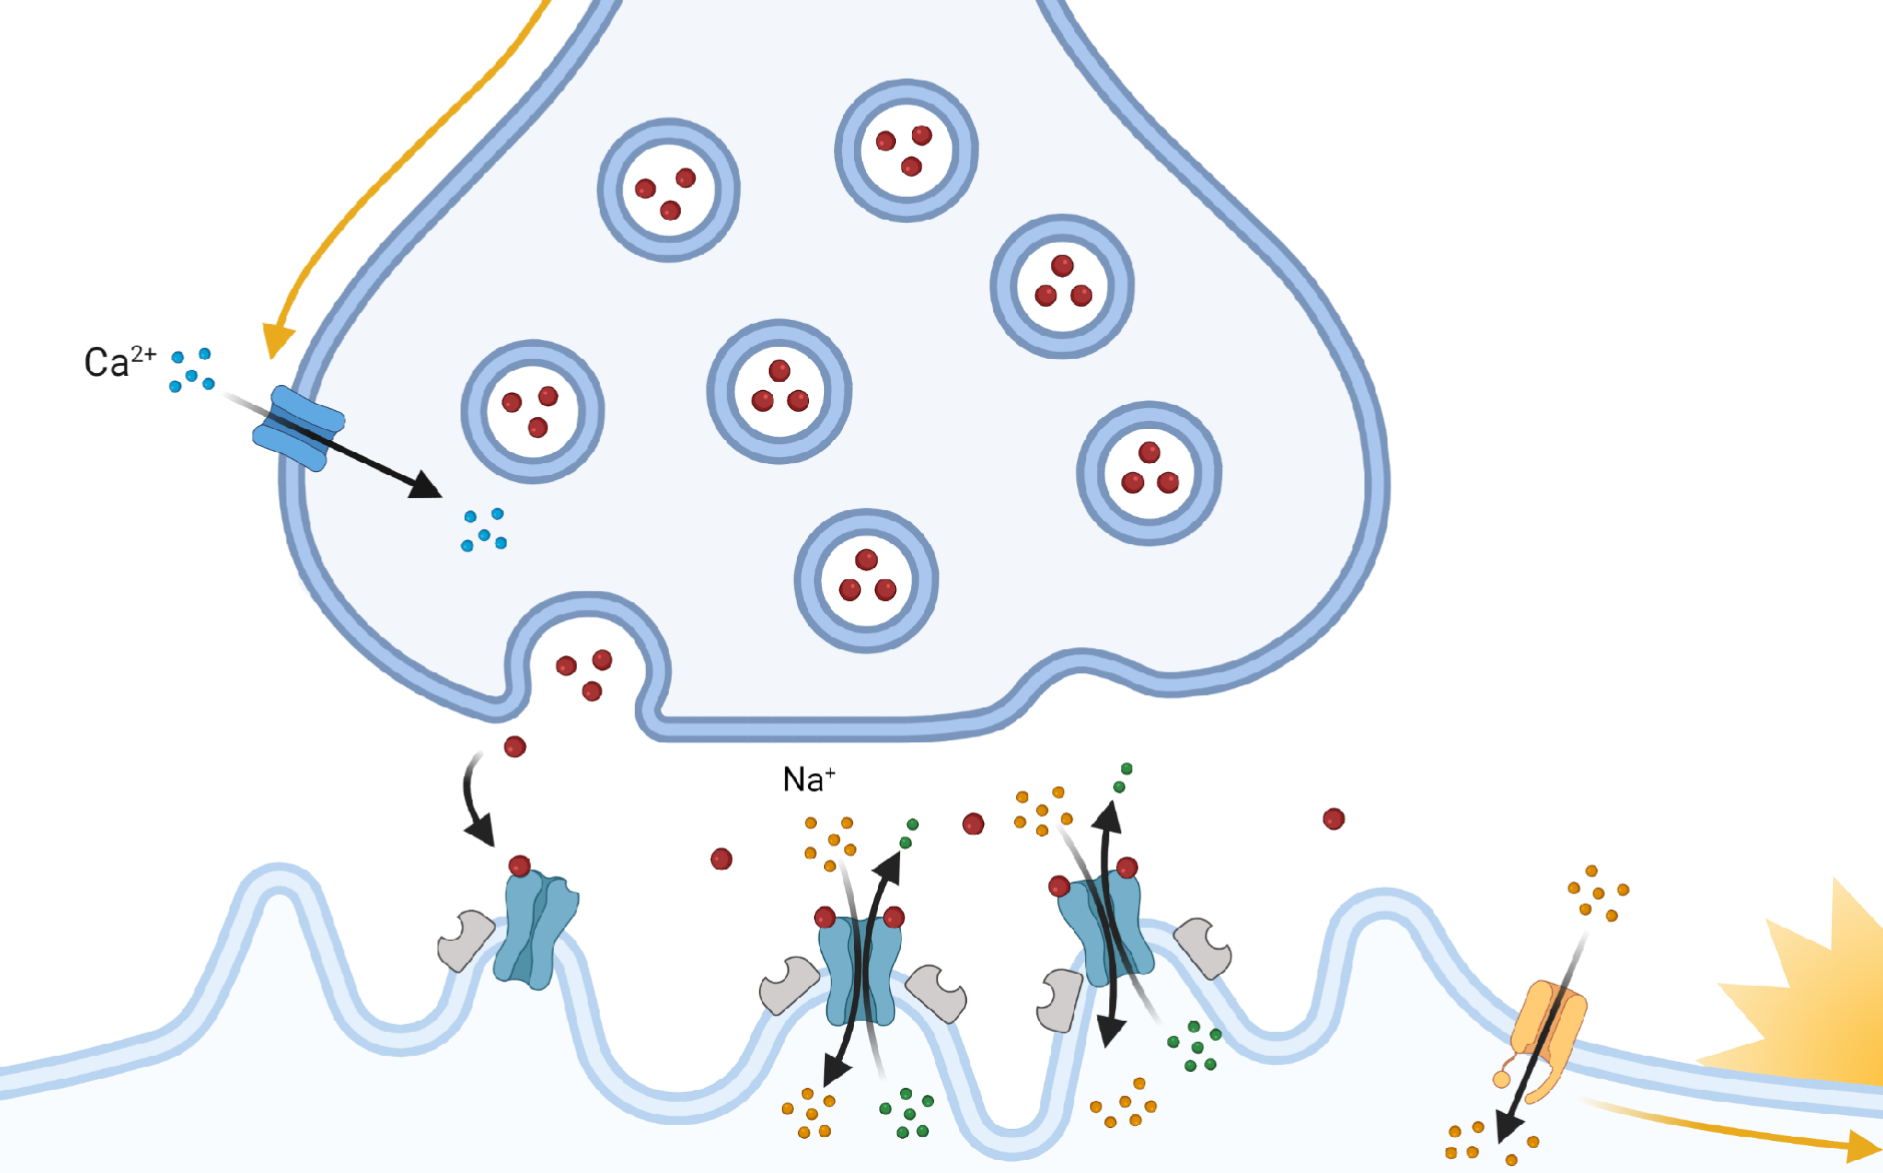
\includegraphics[width=0.65\linewidth]{Pictures/Screenshot 2024-04-03 005847.png}
\end{center}
\begin{enumerate}
    \item Action potential arrives at presynaptic terminal
    \item Voltage gated calcium channels open, allowing influx of calcium cations
    \item Calcium cations allows vesicle docking at acteylcholine (ACh) release
    \item Channels open when 2 ACh bind to each receptor
    \item End-plate potential is generated
    \item Action potential is generated and spreads to muscle fibre
    \item Neurotransmitter is removed by acetylcholinesterase (AChE)
\end{enumerate}

\subsection{Skeletal Muscle Function (Excitation-Contraction Coupling)}
At the neuromuscular Junction and EPP, the action potential get to a core myofibril in muscle fibre cell 

\subsubsection{Excitation}
\begin{enumerate}
    \item Ach release at neuromuscular junction
    \item AP spreads across
entire sarcolemma and
into T-tubules
    \item Calcium cations release by SR into
cytoplasm (sarcoplasm)
    \item Calcium cations binds to
tropomyosin complex
\& causes active sites on
actin filaments to be
exposed
    \item Myosin binds to actin \&
initiates cross bridging
process (muscle
contraction)
\end{enumerate}
\begin{center}
    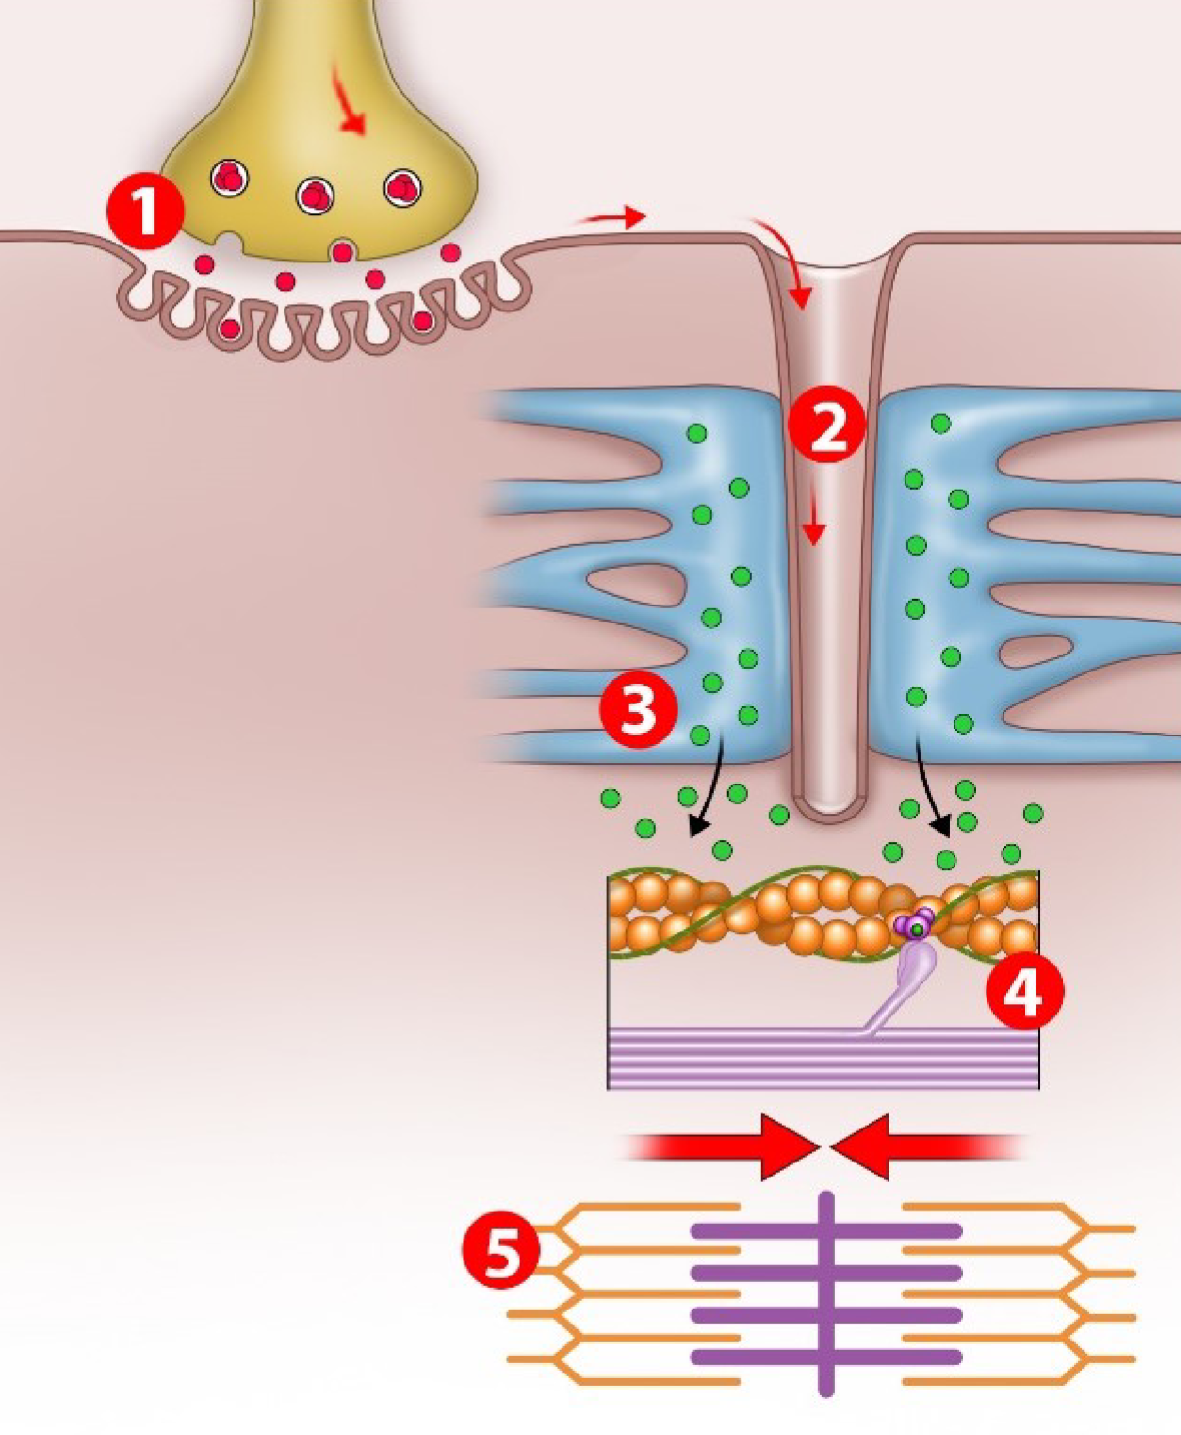
\includegraphics[width=0.7\linewidth]{Pictures/Screenshot 2024-04-03 223557.png}
\end{center}

\subsubsection{Cross-bridge cycle}
\begin{enumerate}
    \item binding
    \begin{itemize}
        \item ATP hydrolysius to ADP
        \item Energized myosin head
        \item Myosin attaches to actin forming cross bridge
    \end{itemize}
    \item bending
    \begin{itemize}
        \item Power stroke
        \item Myosin-actin binding triggers release of stored energy
        \item Myosin pivots (ADP \& Pi released)
        \item Pulls actin to center of sarcomere
    \end{itemize}
    \item detachment
    \begin{itemize}
        \item New ATP binds to myosin
head
        \item Decreases affinity of myosin
for actin
        \item Myosin detaches from actin
filament
    \end{itemize}
    \item energized
    \begin{itemize}
        \item Myosin returned to original
position
        \item ATP hydrolized to ADP \& Pi
        \item Myosin re-energized and
prepares for another binding
cycle
    \end{itemize}
\end{enumerate}
\begin{center}
    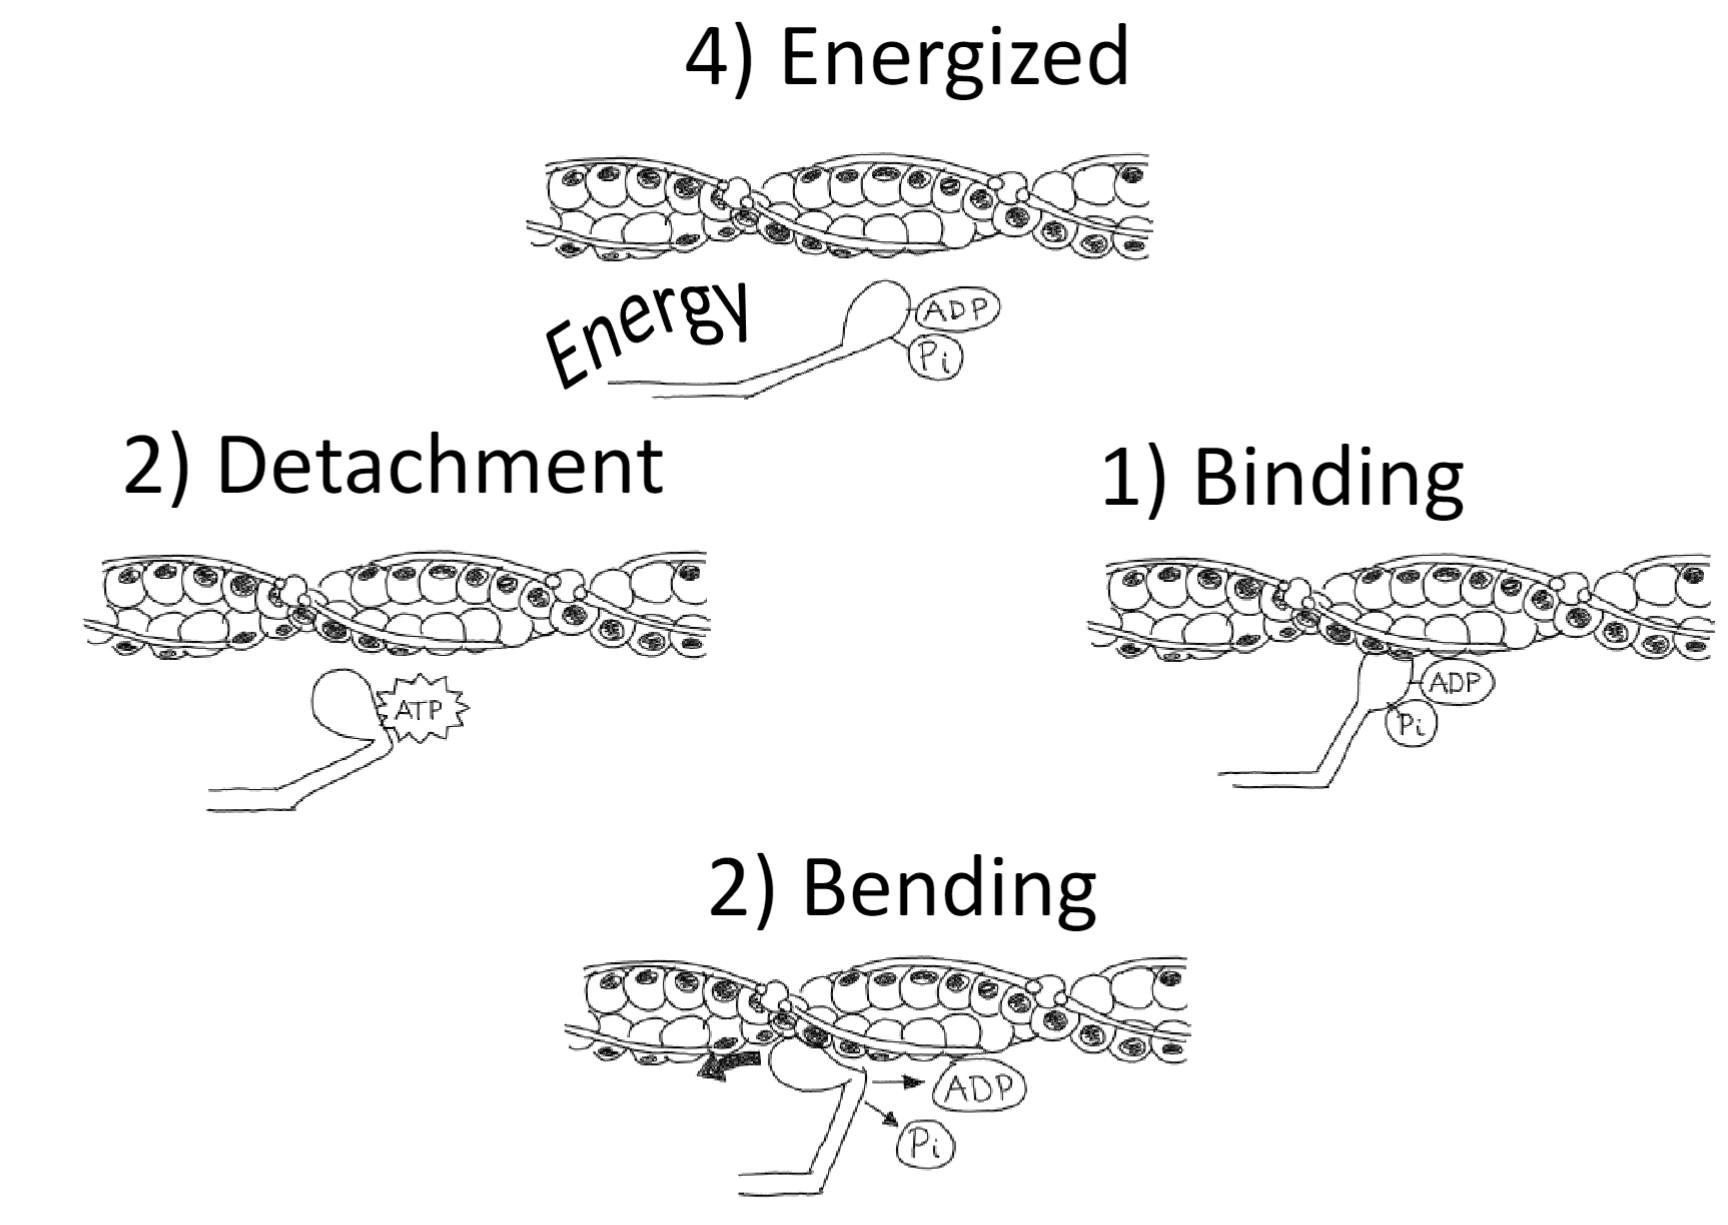
\includegraphics[width=0.65\linewidth]{Pictures/Screenshot 2024-04-03 223633.png}
\end{center}

\subsubsection{Relaxation}
\begin{enumerate}[start=6]
    \item ACh is broken down by
acetylcholinesterase
    \item SR uses ATP-powered pumps
to collect Calcium cations
    \item Tropomyosin complex takes
up myosin binding sites
    \item Cross-bridge binding does not
occur. Compressed Titin recoils
the sarcomere, like a spring
    \item Muscle relaxation occurs
\end{enumerate}

\begin{center}
    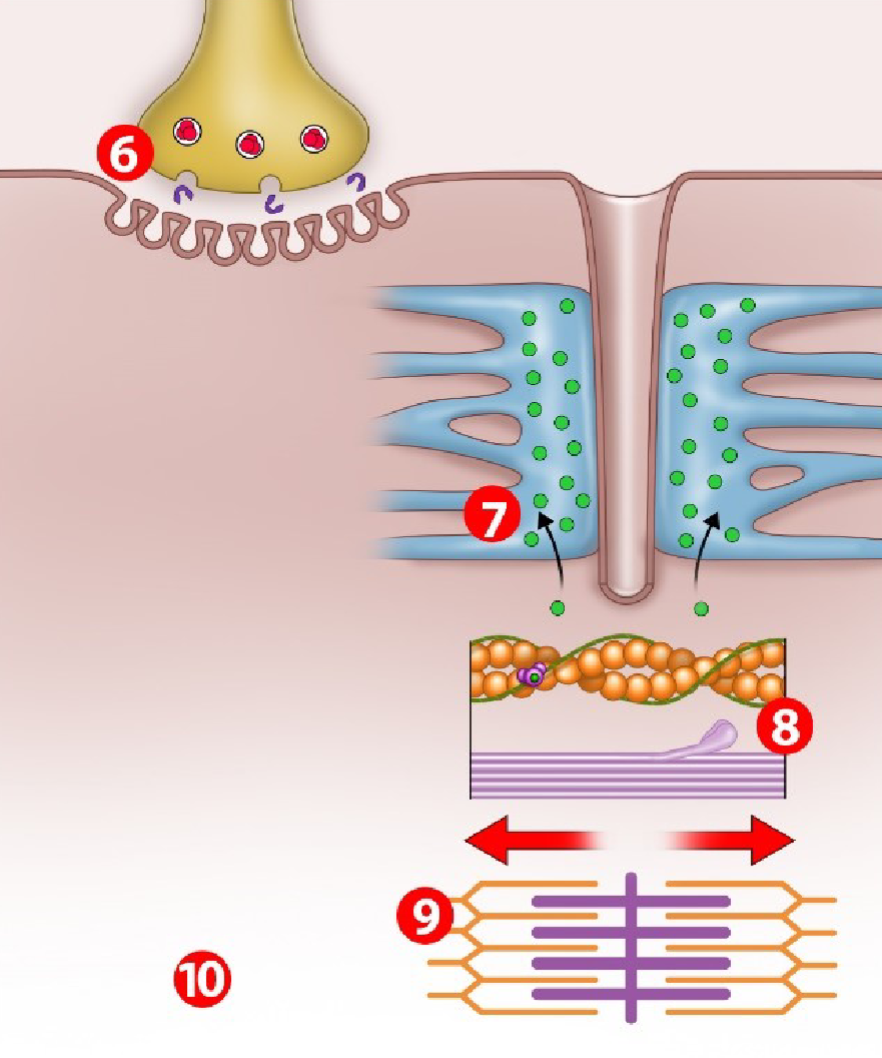
\includegraphics[width=0.31\linewidth]{Pictures/Screenshot 2024-04-03 225216.png}
\end{center}

\begin{exercise}
\begin{tabular}{ccc}
\textbf{lon}  & \textbf{K+}  & \textbf{Na+} \\
\hline
Intracellular (mMol/L) &  90  & 24 \\
Extracellular (mMol/L) &  14  & 130 
\end{tabular}

    Ion concentrations of a
skeletal muscle fiber,
during strenuous exercise,
are shown in the table on
the right. Based on what
you know about typical ion
concentrations, what are
three factors that explain
the ion concentrations
given in the table?
\end{exercise}

\begin{exercise}
    What will happen to the
resting membrane
potential of a skeletal
muscle fiber during
strenuous exercise? Explain in quantitative
terms (using the Nernst
Equation) and in qualitative
terms, the likely
polarization compared to
an unfatigued muscle fiber
that has a resting
membrane potential of -75
mV?
\end{exercise}

\section{Skeletal Muscle Function}
\subsection{Tension Developed by Each Fiber}
\begin{itemize}
    \item Action potential frequency
    \item Fiber strength
    \item Fiber diameter
    \item Fatigue
    \item Fiber type
\end{itemize}

\subsubsection{Action potential frequency}
\begin{figure}[h!]
\begin{center}
    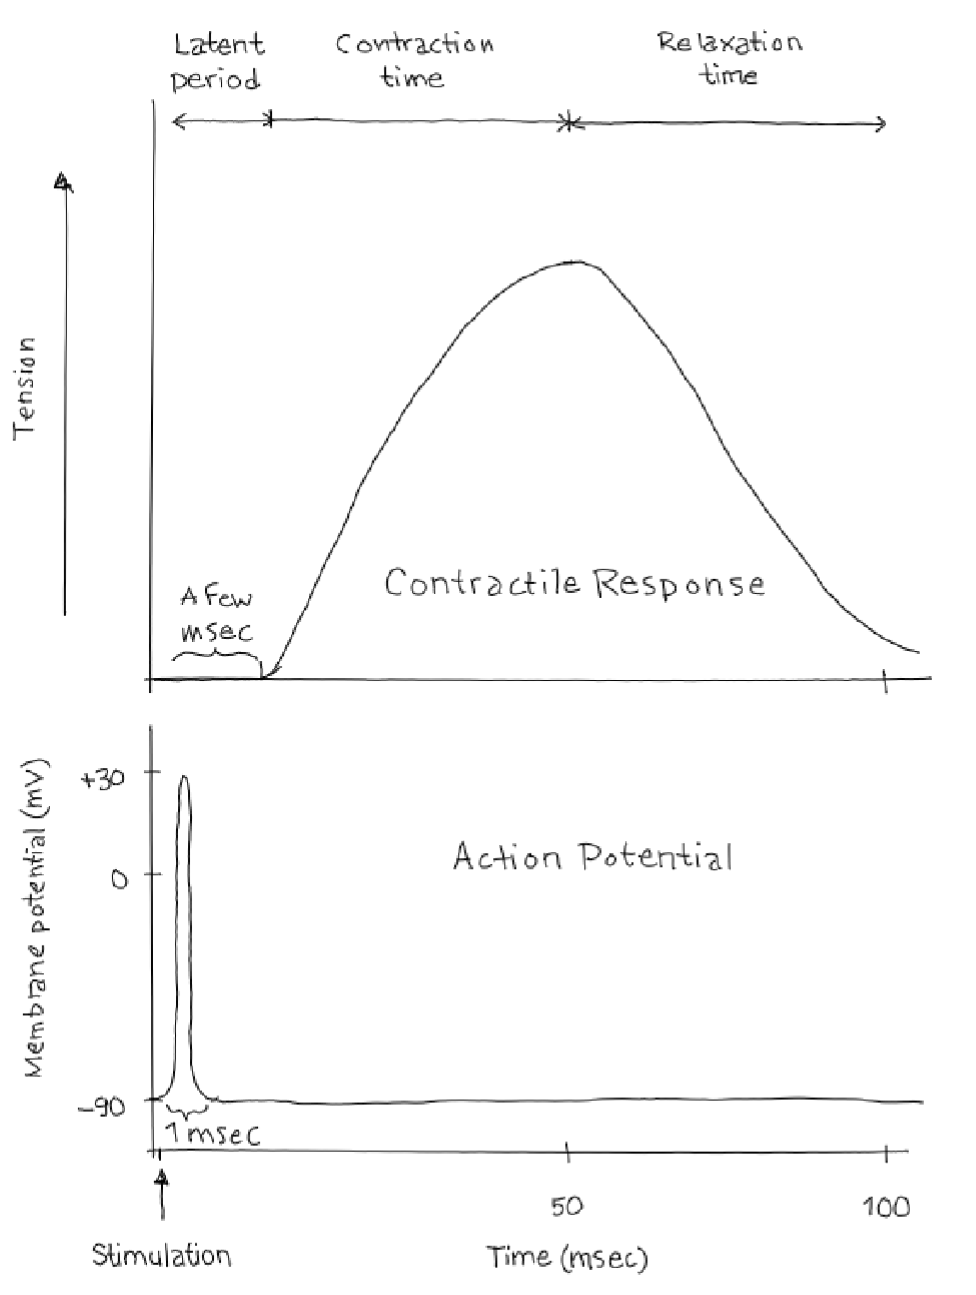
\includegraphics[width=0.5\linewidth]{Pictures/Screenshot 2024-04-03 225713.png}
    \caption{Relationship of action potential to a muscle twitch}
\end{center}
\end{figure}

\begin{remark}
    Muscle is stimulated (i.e. membrane
potential peak) and contractile
response occurs (i.e. twitch)
\end{remark}

\begin{figure}[h!]
\begin{center}
    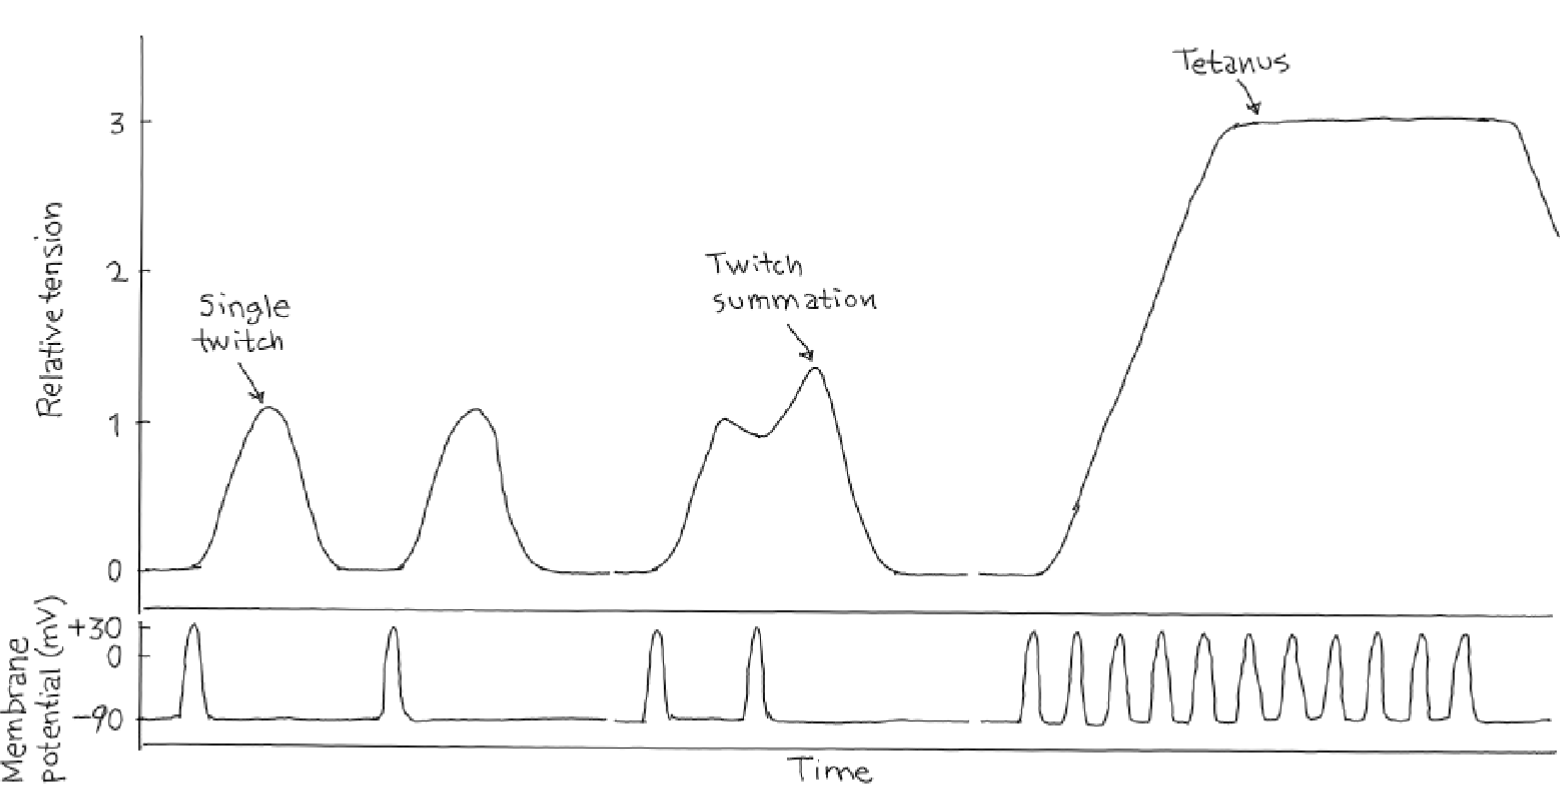
\includegraphics[width=0.65\linewidth]{Pictures/Screenshot 2024-04-03 225826.png}
    \caption{Summation and tetanus}
\end{center}
\end{figure}


\begin{remark}
    Repeated muscle is stimulated (i.e.
membrane potential peaks) creates
prolonged contractile response (i.e.
tetanus)
\end{remark}

\subsubsection{Fiber length}
\begin{figure}[h!]
\begin{center}
    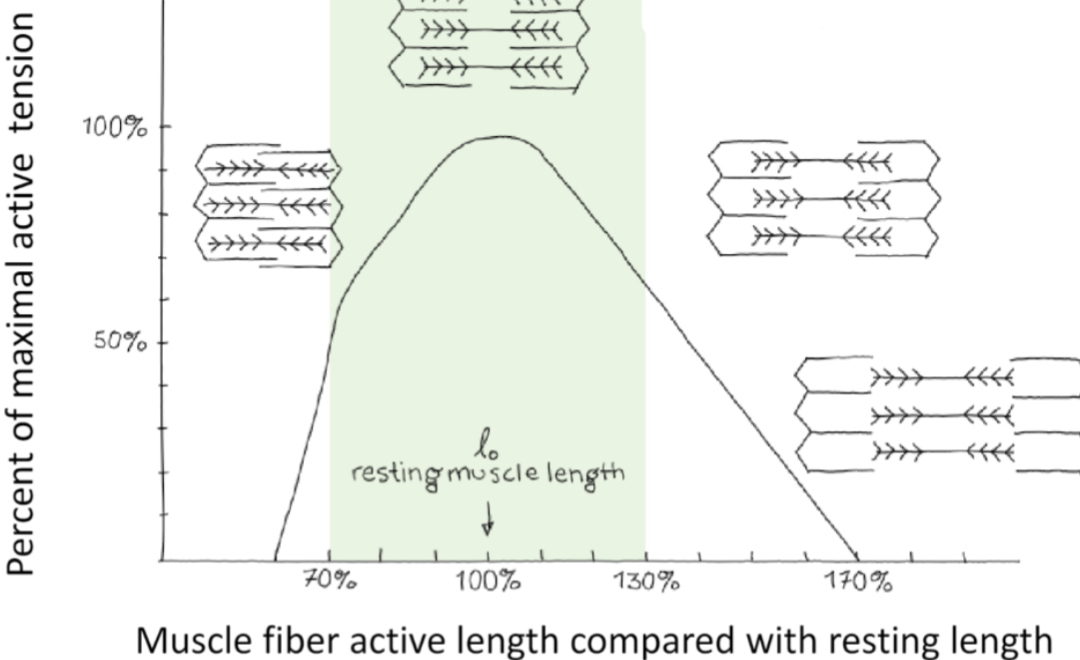
\includegraphics[width=0.4\linewidth]{Pictures/Screenshot 2024-04-03 232654.png}
    \caption{Active Length-Tension Relationship}
\end{center}
\end{figure}


\begin{remark}
    \begin{itemize}
        \item not enough overlap of fibers on the left
        \item too much overlap (resting tension in fiber) on the right
    \end{itemize}
\end{remark}

\begin{remark}
    Consequence: at different
positions (e.g. isometric)
contractile force developed is
different
\end{remark}
\begin{figure}[h!]
\begin{center}
    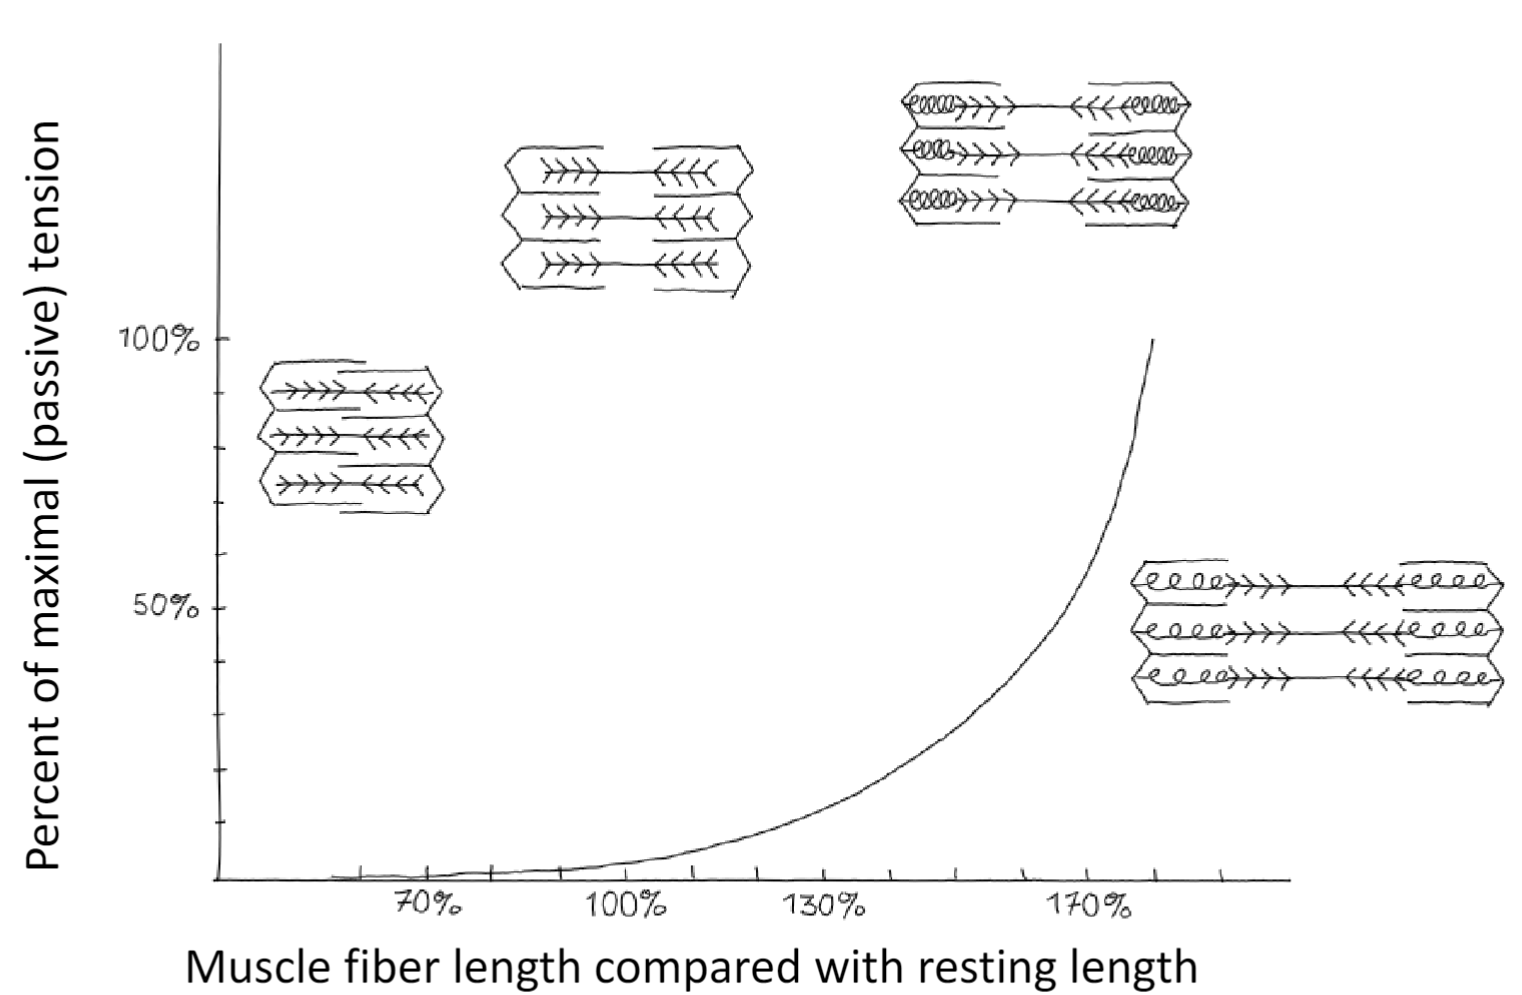
\includegraphics[width=0.6\linewidth]{Pictures/Screenshot 2024-04-03 230713.png}
    \caption{Passive Length-Tension Relationship}
\end{center}
\end{figure}


\begin{remark}
    Consequence: passive force at
different positions helps maintain
posture \& stabilize joints without
active muscle contraction
\end{remark}
\begin{figure}[h!]
\begin{center}
    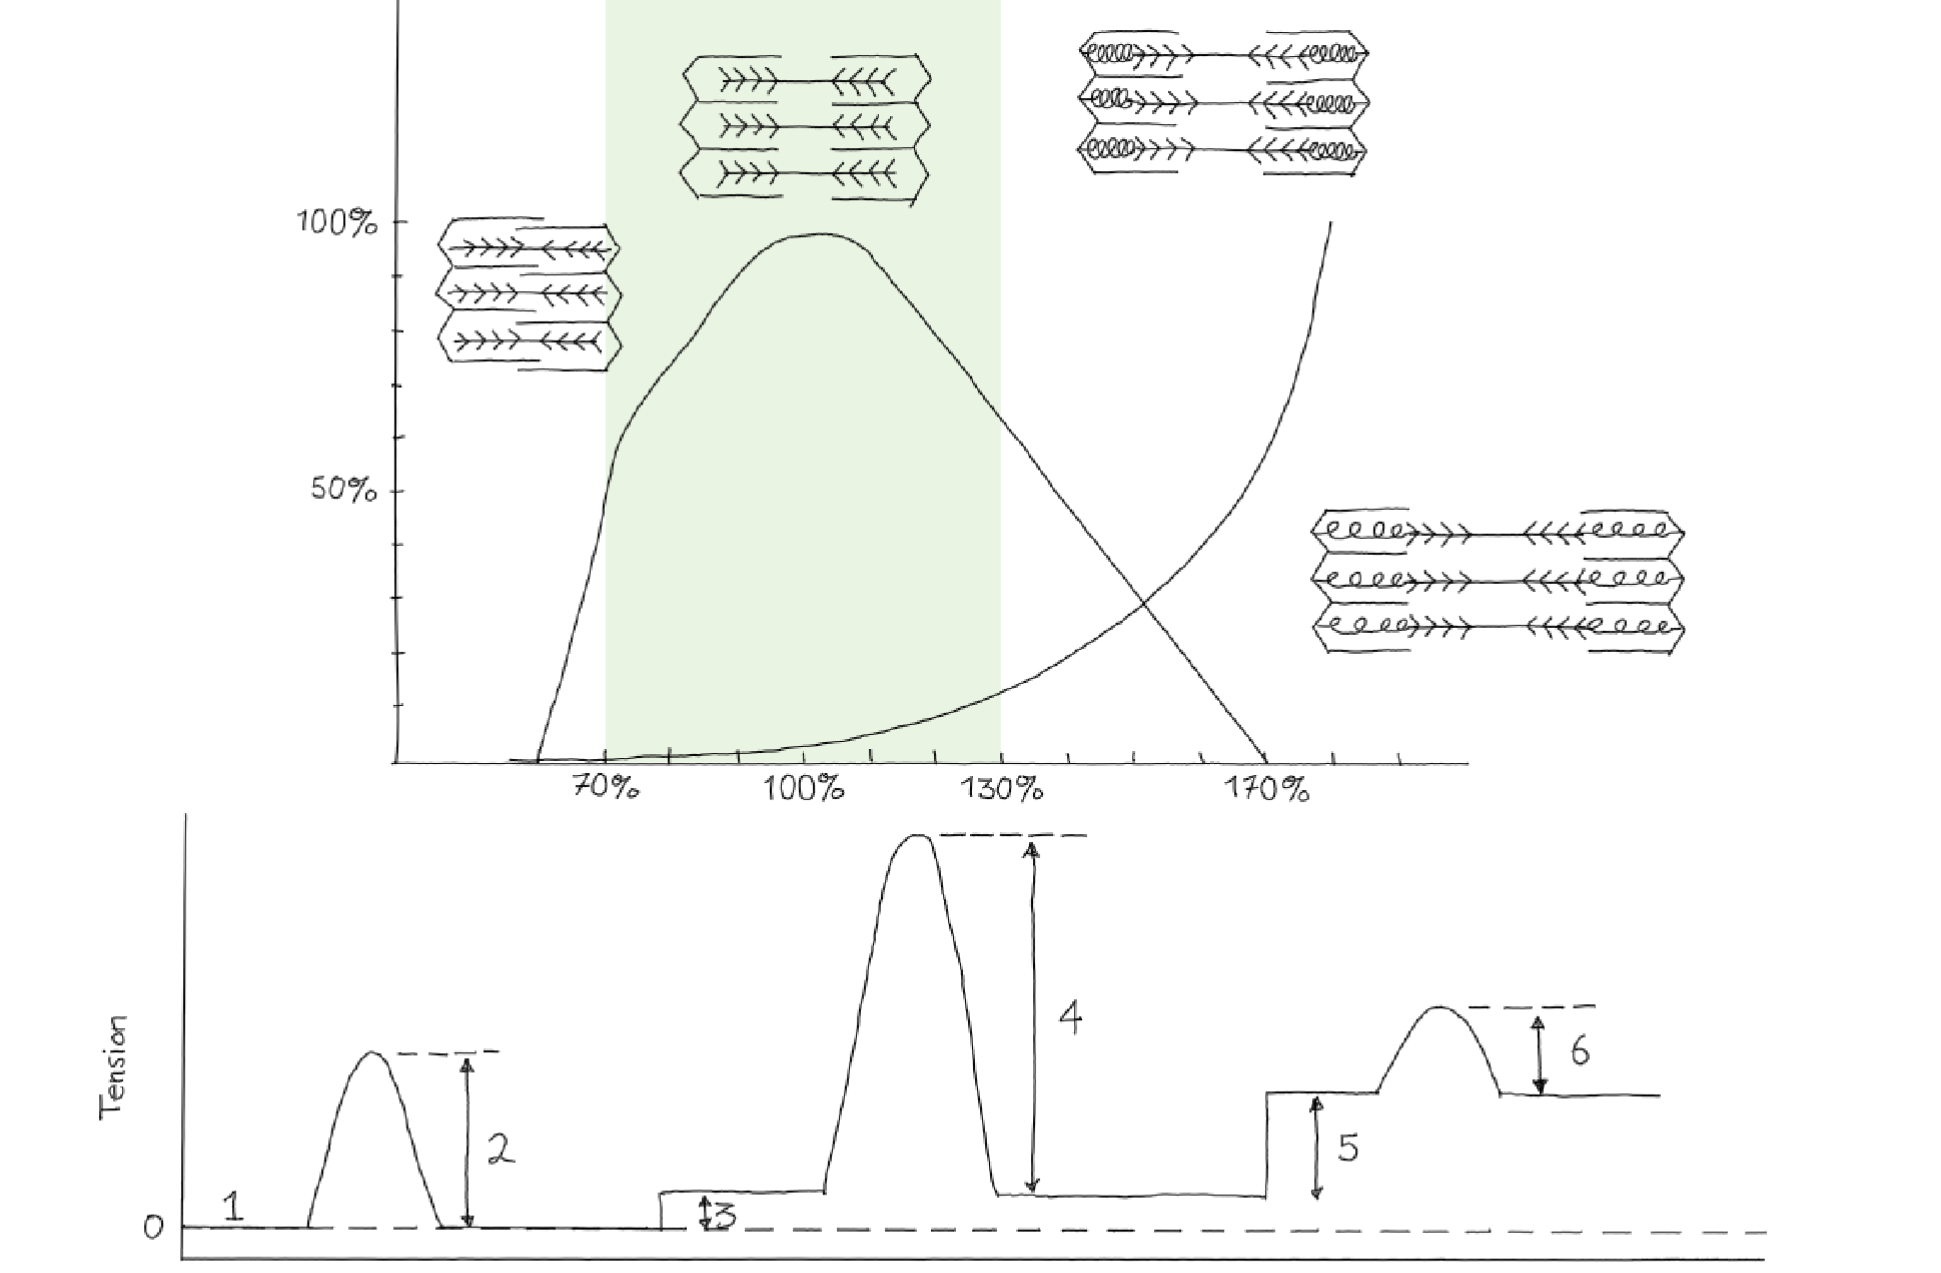
\includegraphics[width=0.85\linewidth]{Pictures/Screenshot 2024-04-03 230817.png}
\caption{ }
\begin{enumerate}
        \item passive at 70\%
        \item active at 70 \%
        \item passive at 100\%
        \item active at 100 \%
        \item passive at 160\%
        \item active at 160 \%
    \end{enumerate}
\end{center}
\end{figure}


\subsubsection{Fiber diameter}
\begin{descriptions}
    \item[Muscle size: ]increased size of muscle fibers
    \item[Debatable: ]increased number of muscle fibers 
\end{descriptions}

\subsubsection{Fatigue}
\textbf{Rate of fatigue development}
\textbf{Types of Contractions}
\begin{figure}[h!]
    \centering
    \begin{subfigure}{0.45\textwidth}
        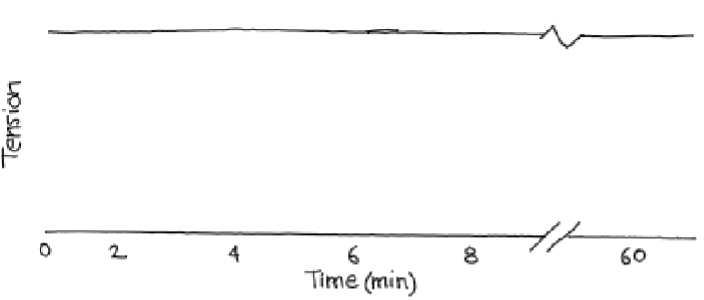
\includegraphics[width=\textwidth]{Pictures/Screenshot 2024-04-03 231435.png}
        \caption{Slow-Oxidative Fibers
(Type 1)}
    \end{subfigure}
    \hfill
    \begin{subfigure}{0.45\textwidth}
        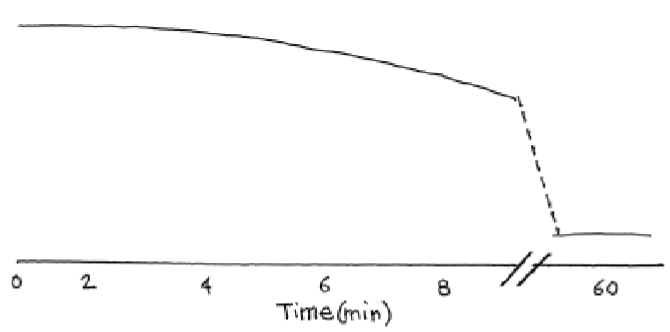
\includegraphics[width=\textwidth]{Pictures/Screenshot 2024-04-03 231440.png}
        \caption{Fast-Oxidative-Glycolytic Fibers
(Type 2A)}
    \end{subfigure}
    \begin{subfigure}{0.45\textwidth}
        \includegraphics[width=\textwidth]{Pictures/Screenshot 2024-04-03 231449.png}
        \caption{Fast-Glycolytic Fibers
(Type 2X)}
    \end{subfigure}
    \caption{}
\end{figure}

\textbf{Other factors that likely influence muscle fatigue}
\begin{itemize}
    \item ADP may interfere with cross-bridge
    \item Accumulation of Lactic acid
    \item Increased extracellular potassium cations
    \item Depletion of glycogen energy reserves
\end{itemize}

\subsubsection{Fiber type}
\begin{tabular}{cccc}
\textbf{Fiber Type} &  \textbf{Diameter} & \textbf{Fatigue Rate} & \textbf{Size of Motor} \\
 & & & \textbf{Neuron Innervating Fiber}\\
\hline
Slow-Oxidative Fibers (Type 1) & Small & Slow & Small \\
Fast-Oxidative-Glycolytic Fibers (Type 2A)  & Largest & Intermediate & Intermediate  \\
Fast-Glycolytic Fibers (Type 2X)  & Large  & Fast  & Large \\
\end{tabular}


\subsection{Tension Developed by
Several Active Fibers}
\begin{itemize}
    \item Number of fibers per motor unit
    \item Number of active motor units
\end{itemize}

\subsubsection{Number of fibers per motor unit}
\begin{figure}[h!]
\begin{center}
    \includegraphics[width=0.6\linewidth]{Pictures/Screenshot 2024-04-03 231449.png}
    \caption{Motor units: more recruitment = more power}
\end{center}
\end{figure}


\subsubsection{Number of active motor units}
\begin{figure}[h!]
\begin{center}
    \includegraphics[width=0.5\linewidth]{Pictures/Screenshot 2024-04-03 232435.png}
    \caption{Different neurons for different
motor units}
\end{center}
\end{figure}

\newpage
\section{Cardiac Muscle ECG and Cycle}
\begin{figure}[h!]
\begin{center}
    \includegraphics[width=0.8\linewidth]{Pictures/Screenshot 2024-04-03 234918.png}
    \caption{ECG}
\end{center}
\end{figure}
\subsection{Electrocardiogram (ECG)}
\textbf{Two-cell Model of the ECG}
\begin{itemize}
    \item 2-cell model to
understand ECG
simplifies cardiac
electrical activity
as two cells (or
groups of cells)
    \item Cell A
    \begin{itemize}
        \item left and right atrium
        \item upper (cranial) two chambers of heart
    \end{itemize}
    \item Cell B
    \begin{itemize}
        \item left and right ventricle
        \item lower (claudal) two heart chambers
    \end{itemize}
    \item 3 possible states for cells A and B
    \begin{itemize}
        \item polarized (resting)
        \item depolarized (active, contraciton)
        \item repolarizing (returning to resting state, relaxing)
    \end{itemize}
\end{itemize}

\begin{figure}[h!]
\begin{center}
    \includegraphics[width=0.5\linewidth]{Pictures/Screenshot 2024-04-03 233656.png}
    \caption{Left side: receives oxygenated
blood from lungs \& sends to body; right side: receives deoxygenated
blood from VC \& sends to lungs
for reoxygenation}
\end{center}
\end{figure}

\begin{figure}[h!]
    \centering
    \begin{subfigure}{0.45\textwidth}
        \includegraphics[width=\textwidth]{Pictures/Screenshot 2024-04-03 234113.png}
        \caption{Notice: Cell A and B
each have a voltage
potential. A is for the left and right atria, and B is for the left and right ventricles. The bottom shows the intracellular voltage from cell \textcolor{blue}{A} to \textcolor{red}{B}}
    \end{subfigure}
    \hfill
    \begin{subfigure}{0.45\textwidth}
        \includegraphics[width=\textwidth]{Pictures/Screenshot 2024-04-03 234130.png}
        \caption{Subtracted action potentials}
    \end{subfigure}
    \begin{subfigure}{0.45\textwidth}
        \includegraphics[width=\textwidth]{Pictures/Screenshot 2024-04-03 234139.png}
        \caption{Extracellular Voltage Moving
Toward Positive Electrode}
    \end{subfigure}
    \begin{subfigure}{0.45\textwidth}
        \includegraphics[width=\textwidth]{Pictures/Screenshot 2024-04-03 234154.png}
        \caption{Extracellular Voltage Moving
Away from Positive Electrode}
    \end{subfigure}
    \caption{}
\end{figure}

\begin{figure}[h!]
\begin{center}
    \includegraphics[width=0.5\linewidth]{Pictures/Screenshot 2024-04-03 234821.png}
    \caption{APs Differ Across Cardiac Cells in
Conduction Network}
\end{center}
\end{figure}

\textbf{Cardiac APs Differ from Neurons \&
Skeletal Muscle}
\begin{itemize}
    \item Specialized ion channels \&
currents in cardiac cells
    \item Rapid depolarization not
followed by quick
repolarization
    \item AP plateaus near 0mV due
to balance between calcium cation
influx \& potassium cation efflux
\end{itemize}
\begin{table}[]
    \centering
\begin{tabular}{cc}
\textbf{Cell}  & \textbf{Velocity (m/s)} \\
\hline
Neuron: Large and myelinated  & 100 \\
Muscle: Skeletal  & 3-5 \\
Muscle: Cardiac  & 0.05-0.4 \\
Muscle: Smooth  & 0.015-0.15 
\end{tabular}
    \caption{Conduction velocity comparison}
    \label{tab:my_label}
\end{table}

\begin{remark}
    Cardiac slower due to
conduction through
gap junctions
\end{remark}


\subsection{Sequence of Depolarization}
\begin{enumerate}
    \item \textbf{Depolarize atria}: Sinoatrial node $\rightarrow$ atrial pathways $\rightarrow$ atrioventricular node
    \begin{enumerate}[start=1]
        \item SA firing: triggers atrial
depolarization (sends
across to left \& throughout
right atrium)
        \item Atrial muscle contracts
        \item AV node: delay/slows
the conduction, allows
atria to fully empty into
ventricles
    \end{enumerate}

\begin{tabular}{ccc}
\textbf{Tissue}  & \textbf{Conduction Velocity (m/s)} \\
\hline
\textbf{SA node}                                  & \textbf{0.05} \\
\textbf{Atrial pathways    }                      & \textbf{1.00} \\
\textbf{AV node     }                             & \textbf{0.05} 
\end{tabular}

    \item \textbf{Depolarize septum from left to right}: Atrioventricular node $\rightarrow$ bundule of his $\rightarrow$ purkinje system
    \begin{enumerate}[start=4]
        \item Bundle of His into
Purkinje fibers: triggers
ventricular
depolarization
    \end{enumerate}

\begin{tabular}{ccc}
\textbf{Tissue}  & \textbf{Conduction Velocity (m/s)} \\
\hline
SA node                                  & 0.05 \\
Atrial pathways                          & 1.00 \\
AV node                                  & 0.05 \\
\textbf{Bundle of His}&\textbf{1.00}\\
\textbf{Purkinje system}&\textbf{4.00}
\end{tabular}

    \item \textbf{Depolarize anteroseptal
region of myocardium
towards apex}: punkinje system $\rightarrow$ ventricular muscle
    \begin{enumerate}[start=5]
        \item ventricular muscle contraction
        \item ventricular muscle relaxation (repolarization)
    \end{enumerate}
\begin{tabular}{ccc}
\textbf{Tissue}  & \textbf{Conduction Velocity (m/s)} \\
\hline
SA node                                  & 0.05 \\
Atrial pathways                          & 1.00 \\
AV node                                  & 0.05 \\
Bundle of His&1.00\\
Purkinje system&4.00\\
\textbf{Ventricular muscle}&\textbf{1.00}
\end{tabular}
    \item \textbf{Depolarize bulk of
ventricular myocardium,
from endocardium to
epicardium}
    \item \textbf{Depolarize posterior
portion of base of
the left ventricle}
    \item \textbf{The ventricles are
now fully depolarized}
    \item \textbf{The ventricles
start to repolarize}
\end{enumerate}

\subsection{Cardiac Filling Action}
\textbf{Major events of left ventricular cardiac cycle}
\begin{figure}[h!]
\begin{center}
    \includegraphics[width=1\linewidth]{Pictures/Screenshot 2024-04-04 001601.png}
    \caption{Diastole: muscle relaxation; systole: coordinated contraction}
\end{center}
\end{figure}

\begin{figure}[h!]
\begin{center}
    \includegraphics[width=0.65\linewidth]{Pictures/Screenshot 2024-04-04 001715.png}
    \caption{Major cardiac cycle events}
\end{center}
\end{figure}

\begin{theorem}
    $SV=EDV-ESV$\\
    $SV$: Stroke volume,  volume of blood (mL)
ejected from the left ventricle
due to contraction of heart
    $EDV$: End Diastole Volume
    $ESV$: End Systole Volume
\end{theorem}

\begin{figure}[h!]
\begin{center}
    \includegraphics[width=0.6\linewidth]{Pictures/Screenshot 2024-04-04 001818.png}
    \caption{}
\end{center}
\end{figure}

\newpage
\section{Cardiac Regulation}
\subsection{Stroke Volume}
\subsubsection{Heart sounds and ECG}
\begin{itemize}
    \item Pressure changes in heart
allow for opening \& closing of
heart valves
    \item \enquote{Lub dub} is an artifact of
turbulence in blood flow
when heart valves snap shut
\end{itemize}
\begin{itemize}
    \item Lub
    \begin{itemize}
        \item Ventriculat systole: First phase of
ventricular contraction
        \item AV valves snap closed: Semilunar valves still
closed
    \end{itemize}
    \item Dub
    \begin{itemize}
        \item Ventricular diastole: Ventricle relaxes \&
pressure falls
        \item Semilunar valves snap closed: AV valves still closed
    \end{itemize}
\end{itemize}

\begin{figure}[h!]
    \centering
    \begin{subfigure}{0.45\textwidth}
        \includegraphics[width=\textwidth]{Pictures/Screenshot 2024-04-04 003419.png}
        \caption{Pressure Changes in the Atria}
    \end{subfigure}
    \hfill
    \begin{subfigure}{0.45\textwidth}
        \includegraphics[width=\textwidth]{Pictures/Screenshot 2024-04-04 003425.png}
        \caption{Pressure Changes in the Ventricles}
    \end{subfigure}
    \begin{subfigure}{0.45\textwidth}
        \includegraphics[width=\textwidth]{Pictures/Screenshot 2024-04-04 003437.png}
        \caption{Pressure Changes in the Aorta}
    \end{subfigure}
    \caption{}
\end{figure}

\begin{figure}[h!]
\begin{center}
    \includegraphics[width=0.6\linewidth]{Pictures/Screenshot 2024-04-04 004121.png}
    \caption{Note: peak
pressures \&
volumes not
identical
}
\end{center}
\end{figure}

\begin{figure}[h!]
\begin{center}
    \includegraphics[width=0.6\linewidth]{Pictures/Screenshot 2024-04-04 004240.png}
    \caption{Effect of heart rate on LV volume. Because much of ventricular filling occurs early in diastole during the rapid filling phase, filling is not seriously impared when diastolic time is reduced as a result of an increase in heart rate}
\end{center}
\end{figure}

\newpage
\subsection{Cardiac Output}
\begin{theorem}
    Two main factors influencing cariac output: Why is stroke volume so important?
    $$CO=SV\times HR$$
    where $CO$ is cardiac output, $SV$ is stroke volume, and $HR$ is heart rate
\end{theorem}

\textbf{Heart Rate Modulation of
Sinoatrial (SA) Nodal Myocyte}
\begin{itemize}
    \item Rate of depolarization
    \item Shift in minimum diastolic potential\
    \item shift in threshold
\end{itemize}

\begin{figure}[h!]
    \centering
    \begin{subfigure}{0.45\textwidth}
        \includegraphics[width=\textwidth]{Pictures/Screenshot 2024-04-04 004646.png}
        \caption{Rate of Depolarization}
    \end{subfigure}
    \hfill
    \begin{subfigure}{0.45\textwidth}
        \includegraphics[width=\textwidth]{Pictures/Screenshot 2024-04-04 004728.png}
        \caption{Shift in Minimum Diastolic Potential}
    \end{subfigure}
    \begin{subfigure}{0.45\textwidth}
        \includegraphics[width=\textwidth]{Pictures/Screenshot 2024-04-04 004744.png}
        \caption{Shift in Threshold}
    \end{subfigure}
    \caption{}
\end{figure}

\subsection{Extrinsic Control of Heart Rate: The Autonomic Nervous System}

\begin{figure}[h!]
\begin{center}
    \includegraphics[width=0.6\linewidth]{Pictures/Screenshot 2024-04-04 004942.png}
\end{center}
    \caption{Autonomic Effects on the Heart}
\end{figure}

\textbf{Parasympathetic Nervous System}

\begin{exercise}
Remember that the Vagus nerve releases ACh.
It turns out that the SA nodal cells have M2
(muscarinic) receptors that respond to ACh. M2
receptors leads to inhibition of target cells.
How might Vagus nerve stimulation change
your heart rate?
\end{exercise}


\begin{figure}[h!]
\begin{center}
    \includegraphics[width=0.6\linewidth]{Pictures/Screenshot 2024-04-04 011648.png}
\end{center}
    \caption{Heart rate decrease with parasympathetic stimulation}
\end{figure}

\textbf{Sympathetic
Nervous System}
\begin{itemize}
    \item Sympathetic nerves releases NE and
cardiomyocytes have $\beta1$ adrenergic receptors.
Recall that agonism of $\beta1$ receptors leads to
excitation of target cells
    \item Conduction velocity increases for the AV node and purkinje fibres, because in the sympathetic $\uparrow=$ $\uparrow$ calcium cations
\end{itemize}

\begin{figure}[h!]
    \centering
    \begin{subfigure}{0.45\textwidth}
        \includegraphics[width=\textwidth]{Pictures/Screenshot 2024-04-04 012102.png}
    \end{subfigure}
    \hfill
    \begin{subfigure}{0.45\textwidth}
        \includegraphics[width=\textwidth]{Pictures/Screenshot 2024-04-04 012129.png}
    \end{subfigure}
    \caption{Heart Rate Increase with
Sympathetic Stimulation}
\end{figure}

\subsection{Autonomic Tone}
There is always the influence of the parasympathetic
and sympathetic nervous systems. That is to say, the
systems do not behave as an “on/off” but rather
“more/less”

\begin{figure}[h!]
\begin{center}
    \includegraphics[width=0.6\linewidth]{Pictures/Screenshot 2024-04-04 012358.png}
\end{center}
    \caption{Vagal and Sympathetic Tone. Intrinsic HR:
HR under
complete
pharmacologic
blockade
}
\end{figure}

\textbf{Calcium cation permeability}
\begin{itemize}
    \item Calcium current: movement of
calcium ions through a cell’s
membrane (recall skeletal
muscle mechanics)
    \item Sympathetic stimulation (i.e., Norepinephrine but
also Epinephrine) enhances Cacium currents and
availability of Calcium cation in the cytosol (cytoplasm) of
ventricular myocytes. These two factors increases the
force developed by ventricular myocytes and the
force of ventricular contraction
\end{itemize}


\begin{figure}[h!]
\begin{center}
    \includegraphics[width=0.6\linewidth]{Pictures/Screenshot 2024-04-04 012811.png}
\end{center}
    \caption{Sympathetic Stimulation on
Stroke Volume
}
\end{figure}

\begin{figure}[h!]
\begin{center}
    \includegraphics[width=0.6\linewidth]{Pictures/Screenshot 2024-04-04 012911.png}
\end{center}
    \caption{Ability of the Heart Muscle to Contract
AKA: Contractility. \textbf{Inotropic effect}: when nervous
system or medication changes
the contractility of the heart
}
\end{figure}

\newpage
\subsection{Summary: Extrinsic Control of Cardiac Output}
\begin{figure}[h!]
\begin{center}
    \includegraphics[width=0.6\linewidth]{Pictures/Screenshot 2024-04-04 013127.png}
\end{center}
    \caption{}
\end{figure}

\section{Blood Vessels and Blood Pressure}
\begin{figure}[h!]
\begin{center}
    \includegraphics[width=0.6\linewidth]{Pictures/Screenshot 2024-04-05 at 5.13.43 PM.png}
\end{center}
    \caption{}
\end{figure}
\subsection{Smooth Muscles}
\begin{descriptions}
    \item[\textcolor{red}{S}kin: ]Arrector pili of skin 
    \item[\textcolor{red}{T}ract: ]GI tract, respiratory tract, reproductive tract, ureters
    \item[H\textcolor{red}{O}llow: ]Walls of stomach, intestine, uterus, bladder
    \item[\textcolor{red}{V}essel: ]Aorta, arteries, arterioles, veins, lymphatic vessels
    \item[\textcolor{red}{E}ye: ] Ciliary muscle, iris
\end{descriptions}
\subsubsection{Smooth muscle versus skeletal muscle}
\begin{itemize}
    \item Skeletal muscle fibers
    \begin{itemize}
        \item long cylindrical fibres
        \item striated
        \item multinucleated
        \item enables movement
    \end{itemize}
    \item Smooth muscle fibers
    \begin{itemize}
        \item short, spindle shaped
        \item non-striated (smooth)
        \item single nucleus
        \item facilitates involuntary processes
    \end{itemize}
\end{itemize}

\subsubsection{Smooth muscle structure}
\begin{figure}[h!]
\begin{center}
    \includegraphics[width=\linewidth]{Pictures/Screenshot 2024-04-05 at 5.19.25 PM.png}
\end{center}
    \caption{\textbf{Skeletal muscle:} attached to bones, quick powerful contraction, respond to nervous system\textbf{Smooth muscle:} in walls of internal organs, slow sustained contractions, cell junctions connect and support function, respond to hormones and nervous system}
\end{figure}

\textbf{Schematic of smooth muscle}
\begin{figure}[h!]
\begin{center}
    \includegraphics[width=0.3\linewidth]{Pictures/Screenshot 2024-04-05 at 5.21.53 PM.png}
\end{center}
    \caption{Recall: sarcolemma (cell membrane); actin (thin); myosin (thick); dense body (anchoring site, like z band); intermediate filament (cytoskeleton filament)}
\end{figure}

\subsubsection{Calcium cation permeability}
\begin{itemize}
    \item Autonomic stimulation (i.e., neurotransmitters)
change the availability of Calcium cations in the cytosol of
smooth muscle cells.
    \item Smooth muscle cells have a sufficient level of Calcium cations
to maintain a low level of tension and are sensitive
to varying degrees of autonomic neurotransmitters
depending on the distribution of cholinergic and
adrenergic receptors
\end{itemize}

\subsubsection{Innervation of smooth muscle}
\begin{descriptions}
    \item[Skeletal muscle: ]Nerve connected by neuromuscular junction
    \item[Smooth muscle: ]Nerve connected by varicosity
    \item[Varicosity: ]\begin{descriptions}
    \end{descriptions} 
    \begin{itemize}
        \item Swelling at end of nerves
        \item Release neurotransmitter into wide synaptic cleft (diffuse
junction)
        \item Neurotransmitter diffuse across clef and affect smooth
muscle cells
        \item SMCs may be far from nerve ending
        \item Allows one nerve ending to impact many SMCs at once
    \end{itemize}
\end{descriptions}
\begin{figure}[h!]
\begin{center}
    \includegraphics[width=0.6\linewidth]{Pictures/Screenshot 2024-04-05 at 5.24.55 PM.png}
\end{center}
    \caption{Innervation of smooth muscle}
\end{figure}

\subsection{Vascular System Structure \& Function}
\textbf{Basic organization of cardiovascular system}
\begin{figure}[h!]
\begin{center}
    \includegraphics[width=0.6\linewidth]{Pictures/Screenshot 2024-04-05 at 5.30.22 PM.png}
\end{center}
    \caption{Basic organization of cardiovascular system, showing the important function characteristics of arteries and veins}
\end{figure}
\subsubsection{Structure of blood vessels}
\begin{descriptions}
    \item[Tunica externa]\begin{descriptions}
    \end{descriptions} 
    \begin{itemize}
        \item structural support
        \item collagen and loose elastic fibers
    \end{itemize}
    \item[Tunica media]\begin{descriptions}
    \end{descriptions} 
    \begin{itemize}
        \item support, change vessel diameter, regulate blood flow
        \item SMC, collagen, elastic tissue
    \end{itemize}
    \item[Tunica intima]\begin{descriptions}
    \end{descriptions} 
    \begin{itemize}
        \item single layer endothelial cells \& connective tissue
        \item release chemicals \& support gas exchange
        \item basement membrane (innermost layer) thin fibrous support for endothelial cells
    \end{itemize}
\end{descriptions}
\begin{figure}[h!]
\begin{center}
    \includegraphics[width=0.6\linewidth]{Pictures/Screenshot 2024-04-05 at 5.31.58 PM.png}
\end{center}
    \caption{Basic organization of cardiovascular system, showing the important function characteristics of arteries and veins}
\end{figure}

\begin{figure}[h!]
\begin{center}
    \includegraphics[width=0.6\linewidth]{Pictures/Screenshot 2024-04-05 at 5.35.38 PM.png}
\end{center}
    \caption{Structure of blood vessels}
\end{figure}

\begin{figure}[h!]
\begin{center}
    \includegraphics[width=0.6\linewidth]{Pictures/Screenshot 2024-04-05 at 5.36.26 PM.png}
\end{center}
    \caption{Different amounts of smooth muscle in arteries and arterioles}
\end{figure}

\begin{figure}[h!]
\begin{center}
    \includegraphics[width=0.6\linewidth]{Pictures/Screenshot 2024-04-05 at 5.39.18 PM.png}
\end{center}
    \caption{Extrinsic Factors Affecting
Diameter of Systemic Arterioles}
\end{figure}

\begin{figure}[h!]
\begin{center}
    \includegraphics[width=0.6\linewidth]{Pictures/Screenshot 2024-04-05 at 5.39.42 PM.png}
\end{center}
    \caption{Extrinsic (\textcolor{red}{and local}) Factors Affecting
Diameter of Systemic Arterioles. \textbf{Myogenic activity: muscular contractile activity}; Endolethin/NO are released by endothelial cells to impact vasodilation/vasocontraction}
\end{figure}
\newpage
\begin{theorem}
    \textbf{Hagen-Poiseuille Equation}
    $$\Delta P=Q\underbrace{\frac{8\eta L}{\pi r^4}}_{TPR}=CO\times TPR$$
    \begin{align*}
        &\Delta P=\text{pressure difference}\\
        &Q=\text{flow}\\
        &r={\rm radius}\\
        &L={\rm length}\\
        &\eta=\text{dynamic viscosity(fluid's internal resistance to flow, in }Pa\cdot s)
    \end{align*}
\end{theorem}

\begin{figure}[h!]
\begin{center}
    \includegraphics[width=0.6\linewidth]{Pictures/Screenshot 2024-04-05 at 5.47.43 PM.png}
\end{center}
    \caption{Factors that alter resistance}
\end{figure}

\begin{figure}[h!]
\begin{center}
    \includegraphics[width=0.6\linewidth]{Pictures/Screenshot 2024-04-05 at 5.48.56 PM.png}
\end{center}
    \caption{Arterioles have the largest pressure drop}
\end{figure}

\begin{figure}[h!]
\begin{center}
    \includegraphics[width=0.6\linewidth]{Pictures/Screenshot 2024-04-05 at 5.49.36 PM.png}
\end{center}
    \caption{Our final flowchart: influence on MAP}
\end{figure}

\begin{figure}[h!]
\begin{center}
    \includegraphics[width=0.6\linewidth]{Pictures/Screenshot 2024-04-05 at 5.50.44 PM.png}
\end{center}
    \caption{Elastic resevoir: heart/vessel coupling}
\end{figure}

\begin{figure}[h!]
\begin{center}
    \includegraphics[width=0.6\linewidth]{Pictures/Screenshot 2024-04-05 at 5.51.24 PM.png}
\end{center}
    \caption{Different Tissues have Opposite Responses
to Sympathetic Nervous System. E: Epinephrine}
\end{figure}

\begin{figure}[h!]
\begin{center}
    \includegraphics[width=0.6\linewidth]{Pictures/Screenshot 2024-04-05 at 5.52.50 PM.png}
\end{center}
    \caption{Blood pressure in the aorta}
\end{figure}







\part{CIN211}
%----------------------------------------------------------------------------------------
%	CHAPTER 3
%----------------------------------------------------------------------------------------
\chapter{Class Notes}
\chapterimage{chapter_head_1.pdf} % Chapter heading image
\section{Early Films}
\subsection{Demolition d’ un mur, Le Voyage dans la lune}
\begin{descriptions}
    \item[Louis Lumiere: Demolition d’ un mur (1895)]
    \begin{descriptions}
    \end{descriptions}
    \begin{itemize}
        \item Early exploration of motion pictures
        \item We cannot travel in time, but film can: Lumiere showed that something broken can be made whole again
    \end{itemize}
    \item[Georges Melies: Le Voyage dans la lune (1902)] 
    \begin{descriptions}
    \end{descriptions}
    \begin{itemize}
        \item First scifi film, very populer
        \item Special effects
        \item ‘Mocking’ scientists, satire, since science is quickly being professionalized
        \item The scientists’ fantasy of themselves, as wizards (Melies think that scientists think highly of themselves)
        \item Colonization of moon, colonial ideas, imperialism of professional science (Melies mocks that)
    \end{itemize}
    \item[The 6th World (2016)]
    \begin{descriptions}
    \end{descriptions}
    \begin{itemize}
        \item What distinguishes mythology and science
        \item What gets to be science and who gets to be a scientist
        \item Scientists think highly of themselves
    \end{itemize}
\end{descriptions}
\section{Entering Modernity}
\subsection{Metropolis (and Cabinet of Dr. Caligari)}
\begin{descriptions}
    \item[The Cabinet of Dr. Caligari and Metropolis]
    \begin{descriptions}
    \end{descriptions}
    \begin{itemize}
        \item How technology has the ability to overturn society
        \item Caligari very theatrical, Metropolis very "blockbuster-y"
        \item German expressionism often a lot about the set
    \end{itemize}
    \item[Mise-en-scene]
    \begin{descriptions}
    \end{descriptions}
    \begin{itemize}
        \item Decor
        \item Set design
        \item Actors
        \item Customing, makeup
        \item Lighting
        \item Special effects
        \item Everything in front of the camera that is \textbf{not} sound or editing (cuts)
    \end{itemize}
    \begin{remark}
        Science fiction is all about \enquote{images of wonder}, only something you can imagine.\\
        Storytelling doesn't necessarily always make sense especially in early sci-fi because films are lost, but the \enquote{images} live on.
    \end{remark}
    \item[German Expressionism]
    \begin{descriptions}
    \end{descriptions}
    \begin{itemize}
        \item Psychological states externalized into film
        \item Arts movement, Avante-garde aesthetic movement: 1910-1927
        \item Graphic shapes (bold)
        \item Chiaroscuro (strong contrasts between light and dark)
        \item Heavy make-up
        \item Shapes are distorted and exaggerated to suggest an emotional state
        \item The world as the hero or another character is experiencing it or imagines it to be
        \item Most often used in horrors or horror-comedies, thrillers
        \item Other similar arts movements at the time:
        \begin{itemize}
            \item Surrealism
            \item Cubism
            \item Bauhaus
        \end{itemize}
    \end{itemize}
    \item[Cesare slinking] 
    \begin{descriptions}
    \end{descriptions}
    \begin{itemize}
        \item Character becomes part of the decor
    \end{itemize}
    \item[Ideas in Metropolis]
    \begin{descriptions}
    \end{descriptions}
    \begin{itemize}
        \item Metropolis not well receipted in Germany, but welcomed in America
        \item How the use of 'scientific' special effects comments on
        \begin{itemize}
            \item Labour and industry
            \item Economic revolution
            \item Gender relations
            \item Family organization
            \item Class dynamics
            \item The concept and experience of the city
        \end{itemize}
        \item Special effects include
        \begin{itemize}
            \item Schufftan process (using mirror to display one image onto another)
            \item Light-filled tubes
            \item Stop-motion animation with minatures
            \item Hand-drawn animation
            \item Multiple exposure (fusion of different images)
        \end{itemize}
        \item Metropolis: 1920s: Factory work
        \begin{itemize}
            \item Machinery and technology has big role in peoples' lives
            \item Automation, people being replaced
            \item Huge divide between upper and lower class (hierarchy, temptation within lower class), seen visually as well in film with visual divisions
            \item Relationship between machines and bodies become central. Notice that machines are named after body parts e.g. heart machine
        \end{itemize} 
        \item Maria and Maria-tron
        \begin{itemize}
            \item Machine-man is a woman
            \item When men went to war, women took the jobs. There is worry about women entering work force
            \item Connection between production and reproduction essential
            \begin{itemize}
                \item Production: labour
                \item Reproduction: family, children, home
            \end{itemize}
            \item Maria's split
            \begin{itemize}
                \item Becomes two different images of femininity: Maria and whore of Babylon
            \end{itemize}
        \end{itemize}
    \end{itemize}
    \begin{remark}
        Interesting that the mediator is also part of the highest class, how you need to have the luxury in the first place to be able to mediate. There must be a heart connecting the head and the hands: the system and class necessary? 
    \end{remark}
    \begin{remark}
        Images of wonder in Metropolis also influenced fantasy cinema, like cartoons and anime. Where else do we see similar pictures?
    \end{remark}
    \begin{remark}
        Metropolis revolutionized film not because of inventing particular techniques, it's about fusing everything together at the same time. I.e. all the special effects.
    \end{remark}
    \begin{remark}
        Choreography difference between portraying the workers at the beginning, robotic movements, not human-like vs. portraying the maria-tron dancing humanly, gracefully in the performance. Note that the power treats workers (humans) like machines, and machines (maria-tron) like a human (Facist Automation?).
    \end{remark}
    \begin{remark}
        In many ways an anti-capitalistic critique. Politics-wised, very socialist. Combining the people in one body. A lot of montages played with at the beginning of the film. Protagonist as saint, antagonist as un-saint: negative portrayal of working class (i.e. the workers breaking the heart machine). Nothing really unites the two classes, like in fascism, they are joined together by blaming the outside (ie. Germans blaming the Jew). The joint doesn't lead to any real solution and in the end nothing is really changed.
    \end{remark}
\end{descriptions}

\begin{exercise}
    What is included in mise-en-scene? What is excluded?
    \begin{itemize}
        \item \textcolor{blue}{\textbf{Included:} Mise-en-scène encompasses elements such as setting, lighting, costume, makeup, staging, and the positioning of characters and props within the frame. It also includes the use of colors, textures, and overall visual composition.}
        \item \textcolor{blue}{\textbf{Excluded:} Mise-en-scène typically does not involve camera movement, editing, or sound. These elements are often considered separately as part of cinematography and editing.}
    \end{itemize}
\end{exercise}

\begin{exercise}
    What is German Expressionism? What is an example of German expressionism in one of the films we studied?
    \begin{itemize}
        \item \textcolor{blue}{\textbf{Definition:} German Expressionism is an artistic movement that emerged in Germany during the early 20th century, characterized by distorted perspectives, chiaroscuro lighting, angular shapes, and a general emphasis on expressing emotional and psychological states over realistic representation.}
        \item \textcolor{blue}{\textbf{Example in Film:} \textit{The Cabinet of Dr. Caligari} (1920) directed by Robert Wiene is a classic example of German Expressionist cinema.}
    \end{itemize}
\end{exercise}

\begin{exercise}
    What is a \enquote{fascist automation}?
        \begin{itemize}
            \item \textcolor{blue}{\textbf{Definition:} A "fascist automaton" refers to a representation of a machine or robot in the context of a fascist ideology. It often symbolizes control, conformity, and the dehumanization of individuals within a totalitarian regime.}
        \end{itemize}
\end{exercise}

\begin{exercise}
    What is an \enquote{image of wonder}?
        \begin{itemize}
            \item \textcolor{blue}{\textbf{Definition:} An "image of wonder" refers to a visual or cinematic element that evokes a sense of awe, amazement, or astonishment. It is often associated with breathtaking visuals or extraordinary events that captivate the audience.}
        \end{itemize}
\end{exercise}

\begin{exercise}
    Name at least three special effects in \textit{Metropolis}
        \begin{itemize}
            \item \textcolor{blue}{Miniature models of the cityscape.}
            \item \textcolor{blue}{Stop-motion animation for certain scenes.}
            \item \textcolor{blue}{Back projection techniques for combining live-action with pre-filmed backgrounds.}
        \end{itemize}
\end{exercise}

\begin{exercise}
    Give one reason that the machine is conceptually based on the feminine.
        \begin{itemize}
            \item \textcolor{blue}{\textbf{Reason:} The machine in \textit{Metropolis} is conceptually based on the feminine because it represents a fusion of technology and biology. The machine, particularly the Maria-like android, embodies both mechanical and human characteristics, blurring the lines between the artificial and the organic.}
            \item \textcolor{blue}{\textbf{Exploration of Gender Roles:} The decision to craft the machine in a female likeness allows the film to explore and challenge traditional gender roles. It brings attention to societal expectations and the intersection of technology with gender dynamics, reflecting the anxieties and aspirations of the era in which the film was produced.}
        \end{itemize}
\end{exercise}

\begin{exercise}
    Give one reason for biblical iconography in metropolis.
        \begin{itemize}
            \item \textcolor{blue}{\textbf{Reason:} One reason for biblical iconography in \textit{Metropolis} is the film's exploration of themes related to class struggle and social inequality. The biblical references, such as the Tower of Babel, are used to underscore the hubris of the upper class and the consequences of their exploitation of the lower class.}
        \end{itemize}
\end{exercise}


\section{Disaster Aesthetics}
\subsection{Godzilla}
\begin{itemize}
    \item \textbf{Genre Conventions}
    \begin{itemize}
        \item Iconography (ie. spaceships)
        \item Narrative patterns, themes, or tropes
        \item stylistics (a form of presentation, ie. white transitions between interview scenes, special effects in general)
    \end{itemize}
    \item \textbf{Genres are...}
    \begin{itemize}
        \item Reflective (have to be repeated again and again)
        \item Ritualistic and 
        \item Have social functions
    \end{itemize}
    \item \textbf{The social functions of genre}
    \begin{itemize}
        \item Reaffirm cultural values in a predictable way (In Godzilla, the fisherman talk about how breaking culture and tradition is taboo and can cause harm)
        \item Exploit ambivalent social values and attitudes (In Godzilla, it reaffirms social order by purging threatening elements from within society, equivocate on the inherent morality of a society governed by scientific rationality, monster as a symbol for the atomic bombs)
        \item Respond to social trends
        \item Reflect pervasive doubts and anxieties
        \item A deliberate effort to treat a social issue (In Godzilla, we address the bombs dropped in Japan and the threat of nuclear warfare)
    \end{itemize}
    \item \textbf{Hiroshima and Nagasaki Atomic Bombings}
    \begin{itemize}
        \item Two atomic bombs were dropped on the Japanese cities Hiroshima and Nagasaki
on August 6 and 9, 1945
        \item Hiroshima deaths: 140,000 by end of 1945
        \item Nagasaki deaths: 74,000 by end of 1945
        \item Survivors faced widespread injuries and illness due to radiation. These effects last for decades
        \item 90\% of physicians and nurses were killed or injured in Hiroshima
        \item Razed and burnt 70\% of buildings
        \item These disasters added to intensive bombing upon other Japanese cities during the
war and effects of natural disasters
    \end{itemize}
    \item \textbf{Susan Sontag:}
    \begin{itemize}
        \item \enquote{Science fiction films are not about science. They are about disaster, which is
one of the oldest subjects of art. In science fiction films disaster is rarely
viewed intensively; it is always extensive. It is a matter of quantity and
ingenuity. If you will, it is a question of scale. But the scale … does raise the
matter to another level}
        \item \enquote{The aesthetics of destruction, with the particular beauties to be found in
wreaking havoc [are] the core of good science fiction film}
    \end{itemize}
    \begin{remark}
        Why do images of mass destruction (esp. in globally-
recognized cities) give us visual pleasure in the cinema?
    \end{remark}
    \item \textbf{Science as \enquote{Pharmakon}}
    \begin{itemize}
        \item A Greek word that can be translated as remedy, poison, and scapegoat
        \item A both-and concept developed by French philosopher Jacques Derrida (he originally uses it to describe writing)
        \item Yoav Rinon: \enquote{It is both a remedy, as the city's existence in a time of crisis, especially in time of plague,
depends on it; and a poison, since that kind of existence is an outcome of the scapegoat's
expulsion and, sometimes, death.}
        \item Consider: How does the disaster film treat science or tech as an all-of-the-above remedy,
poison, and scapegoat for social ills?
    \end{itemize}
    \item \textbf{Godzilla is...}
    \begin{itemize}
        \item The bomb
        \item The victim
        \item Survivor
    \end{itemize}
    \item \textbf{Shot distances}
    \begin{itemize}
        \item longer shots show destruction
        \item shorter and closer shots show emotion
        \item note there was a fair distribution of all shots in Godzilla, two separate stories going on, the front end disaster and the back end love triangle
    \end{itemize}
    \item \textbf{Film sounds}
    \begin{itemize}
        \item Diegetic (within context of story, can be heard by characters) vs. non-diegetic
        \item Synchronic vs. non-synchronic
        \item Internal (ie. inside someone's head) vs. external 
        \item Acousmatic (visual source cannot be seen, ie. voice from a radio) vs. visualized (can see source)
    \end{itemize}
\end{itemize}
\begin{remark}
    Often in scifi scientists are antagonized (science can be exploited), here Godzilla provides an interesting perspective, how there is sympathy, the creator of the oxygen destroyer, similar to Oppenheimer being the destroyer or worlds. Science is "pharmacon", both poison and remedy. Note image of scientist changes. Important: film not written by the victors, political relevance?
\end{remark}
\begin{remark}
    Genre is always result of culture and history
\end{remark}

\begin{exercise}
What are two qualities of genre?
\begin{itemize}
\item \textcolor{blue}{Reflective (have to be repeated again and again)}
\item \textcolor{blue}{Ritualistic}
\end{itemize}
\end{exercise}

\begin{exercise}
What are three social functions of genre?
\begin{itemize}
\item \textcolor{blue}{Reaffirm cultural values in a predictable way}
\item \textcolor{blue}{Exploit ambivalent social values and attitudes}
\item \textcolor{blue}{Respond to social trends}
\end{itemize}
\end{exercise}

\begin{exercise}
What are the names of the shot distances?
\begin{itemize}
\item \textcolor{blue}{Long shots/ Wide shots}
\item \textcolor{blue}{Medium shots}
\item \textcolor{blue}{Close-ups}
\end{itemize}
\end{exercise}

\begin{exercise}
What does Sontag say that sf films are really about?
\begin{itemize}
\item \textcolor{blue}{Sontag argues that science fiction films are primarily about disaster, exploring the aesthetics of destruction on a grand scale.}
\end{itemize}
\end{exercise}

\begin{exercise}
What are the names of types of film sound?
\begin{itemize}
\item \textcolor{blue}{Diegetic vs. non-diegetic}
\item \textcolor{blue}{Synchronous vs. asynchronous}
\item \textcolor{blue}{Internal vs. external}
\item \textcolor{blue}{Acousmatic vs. visualized}
\end{itemize}
\end{exercise}

\begin{exercise}
What are two ways we know that Godzilla mediates the atomic disaster?
\begin{itemize}
\item \textcolor{blue}{Godzilla's origins as a mutated creature directly reference the effects of nuclear radiation.}
\item \textcolor{blue}{The film's themes of destruction, widespread suffering, and the dangers of scientific advancement mirror the anxieties of post-atomic bomb Japan.}
\end{itemize}
\end{exercise}

\begin{exercise}
What is one way that Japanese monster films depart from American monster films, generally speaking?
\begin{itemize}
\item \textcolor{blue}{Japanese monster films often portray the monsters with a degree of sympathy or ambiguity, reflecting Japan's unique experience with nuclear devastation. American monster films tend to present monsters as purely destructive threats.}
\end{itemize}
\end{exercise}

\subsection*{"The Imagination of Disaster" by Susan Sontag}
\begin{enumerate}[label=\arabic*.]
    \item \textbf{Structure of Science Fiction Films:}
    \begin{itemize}
        \item Sontag notes that typical science fiction films follow predictable patterns, much like westerns. She outlines a model scenario with five phases.
    \end{itemize}

    \item \textbf{Model Scenario:}
    \begin{enumerate}[label=(\roman*)]
        \item The arrival of a threatening entity or force, witnessed by a young scientist who struggles to convince others.
        \item Confirmation of the threat with destructive acts. Attempts at peaceful resolution fail, leading to mass casualties.
        \item National and international response to the crisis, with conferences between scientists and the military. Plans for destroying the enemy are made.
        \item Escalation of atrocities, unsuccessful counter-attacks, and a final strategy involving a powerful weapon. The enemy is repulsed.
        \item Concluding scenes with mutual congratulations, as the hero and his girlfriend wonder if the threat is truly over.
    \end{enumerate}

    \item \textbf{Variations in Scripts:}
    \begin{itemize}
        \item Sontag describes a simpler, lower-budget script with four phases, often involving a hero facing a threat alone and discovering the enemy's vulnerability.
    \end{itemize}

    \item \textbf{Different Themes:}
    \begin{itemize}
        \item Various scenarios involve monstrous transformations caused by scientific experiments, nuclear testing leading to global catastrophe, or space exploration revealing threats to other planets.
    \end{itemize}

    \item \textbf{Aesthetics of Destruction:}
    \begin{itemize}
        \item Sontag argues that science fiction films are not primarily about science but about disaster. She emphasizes the aesthetic appeal of destruction, with a focus on quantity, ingenuity, and scale.
    \end{itemize}

    \item \textbf{Imagery and Sensuous Elaboration:}
    \begin{itemize}
        \item Science fiction films use images and sounds to allow viewers to experience the fantasy of catastrophic events. The emphasis is on sensuous elaboration, creating a visual and auditory spectacle.
    \end{itemize}

    \item \textbf{Importance of Budget and Technology:}
    \begin{itemize}
        \item Sontag mentions the importance of budget and technology in creating visually compelling science fiction films. Widescreen color films, with well-designed model environments, contribute to the genre's impact.
    \end{itemize}

    \item \textbf{Aesthetics of Destruction:}
    \begin{itemize}
        \item The core of a good science fiction film, according to Sontag, lies in the imagery of destruction. The essay suggests that the aesthetics of wreaking havoc and making a mess are central to the genre.
    \end{itemize}
    \item \textbf{Primitive Gratifications and Shared Themes:}
    \begin{itemize}
        \item Certain primitive gratifications in science fiction films, such as depicting urban disaster on a magnified scale, are shared with other film genres. The depiction of mass havoc in old horror and monster films is visually similar to science fiction films, with the difference being primarily in scale.
    \end{itemize}

    \item \textbf{Similarity with Old Monster Films:}
    \begin{itemize}
        \item Sontag draws parallels between the destruction scenes in old monster films, such as King Kong (1933), and those in science fiction films of the 1950s. The archetype of monsters wreaking havoc in a great city remains consistent, with destruction scenes in various science fiction films mentioned.
    \end{itemize}

    \item \textbf{Familiar Themes and Grimness in 1950s Science Fiction Films:}
    \begin{itemize}
        \item Science fiction films of the 1950s take up familiar themes found in 1930s movie serials, comics, and superhero stories. However, Sontag notes a distinct grimness in modern science fiction films, possibly influenced by the enlarged imagination of disaster in contemporary reality.
    \end{itemize}

    \item \textbf{Fantasy of Disaster and Moral Simplification:}
    \begin{itemize}
        \item The lure of fantasizing about disaster lies in its release from normal obligations. End-of-the-world movies, such as "The Day the Earth Caught Fire" (1962), present scenes of deserted metropolises, offering a fantasy of starting anew. Science fiction films also provide extreme moral simplification, allowing the audience to explore cruel or amoral feelings.
    \end{itemize}

    \item \textbf{Moralistic and Aesthetic View of Destruction:}
    \begin{itemize}
        \item Science fiction films are strongly moralistic, often conveying messages about the proper use of science. The films offer a dispassionate, aesthetic view of destruction and violence, emphasizing a technological perspective. Objects and machinery play a major role, embodying a greater range of ethical values than the characters.
    \end{itemize}

    \item \textbf{Scientific Enterprise and Morality:}
    \begin{itemize}
        \item The scientist in science fiction films is often depicted as morally ambivalent, with an emphasis on the proper and humane use of science versus the mad or obsessional use of science. This moralistic theme is shared with classic horror films of the 1930s, such as "Frankenstein" and "Dr. Jekyll and Mr. Hyde."
    \end{itemize}

    \item \textbf{Ambivalence Toward Scientists:}
    \begin{itemize}
        \item Scientists in science fiction films are susceptible to cracking up or going off the deep end. Ambivalence toward scientists is evident, and even sympathetic treatment is conditional on the utility of their scientific endeavors. Intellectual curiosity is often portrayed as a maniacal dementia, cutting scientists off from normal human relations.
    \end{itemize}

    \item \textbf{Contemporary Mistrust of the Intellect:}
    \begin{itemize}
        \item There is a contemporary mistrust of the intellect in science fiction films, particularly directed at the scientist-as-intellectual. The scientist who releases uncontrollable forces is portrayed as a potential threat, and the creative scientist may become a martyr to his own discovery.
    \end{itemize}

    \item \textbf{Changed Proportions in Attitudes:}
    \begin{itemize}
        \item Sontag notes a change in proportions regarding attitudes toward scientists in contemporary science fiction films. While scientists are still treated as both satanists and saviors, the context has shifted, and the scientist's sphere of influence is no longer local but planetary and cosmic.
    \end{itemize}
    
    \item \textbf{Nuclear Trauma and Exorcism:}
    \begin{itemize}
    \item Many science fiction films, particularly in Japanese cinema, reflect a collective trauma related to nuclear weapons and the fear of future nuclear wars.
    \item The awakening of super-destructive monsters often serves as a metaphor for the atomic bomb, with explicit references to nuclear warfare and its consequences.
    \item Themes of contamination, destruction, and global catastrophe permeate narratives, attempting to exorcise the anxieties surrounding nuclear technologies.
    \end{itemize}
\item \textbf{Radiation and Casualties:}
\begin{itemize}
    \item Radiation casualties and the concept of the world as a casualty of nuclear testing are central to science fiction film narratives.
    \item Universes become expendable, worlds become contaminated, burnt out, and obsolete, reflecting deep anxieties about the consequences of nuclear technology.
\end{itemize}

\item \textbf{Wishful Thinking and Imagery of War:}
\begin{itemize}
    \item Science fiction films often feature wishful thinking, including a desire for a "good war" devoid of moral problems.
    \item Imagery of war, including dogfights and escalating firepower, satisfies both bellicose and pacifistic desires, projecting a fantasy of united warfare and international cooperation.
\end{itemize}

\item \textbf{Dehumanization and Anxiety:}
\begin{itemize}
    \item Themes of dehumanization, symbolized by alien invaders seeking to take over humanity, reflect anxieties about the impersonal and depersonalizing conditions of modern urban life.
    \item The fear of losing individuality to a mechanized, emotionless existence is a recurring motif in science fiction films, portraying a struggle against the erasure of humanity.
\end{itemize}

\item \textbf{Fantasy as Coping Mechanism:}
\begin{itemize}
    \item Science fiction films, serving as a popular mythology, allow individuals to cope with the anxieties of banality and inconceivable terror through fantasy.
    \item The films normalize psychologically unbearable scenarios, providing a temporary escape while also inuring audiences to the depicted terrors.
\end{itemize}

\item \textbf{Complicity with the Abhorrent:}
\begin{itemize}
    \item Science fiction films, inadvertently or not, are in complicity with the abhorrent by neutralizing and making unthinkable scenarios more palatable.
    \item The films perpetuate clichés about identity, power, knowledge, and guilt, raising moral questions about the act of "thinking about the unthinkable" in a fantastical context.
\end{itemize}
\end{enumerate}

\section{The Future}
\subsection{La Jetee}
\begin{itemize}
    \item \textbf{Primal Scene:}
    \begin{itemize}
        \item Freudian term
        \item The sight or fantasy of the sight of one's parents having sex
        \item It addresses the question: "where do I come from?"
        \item \textit{Terminator} series exploits this
        \begin{itemize}
            \item Terminator (evil machine from dystopian future) sent back in time to kill
the mother (Sarah Connor) of the leader of the human resistance to the
terminators
            \item Member of the human resistance (Kyle Reese) also sent back to protect
Sarah
            \item  Sarah and Kyle sleep together and conceive John Connor (future leader of
resistance)
            \item  In the future, John selects Kyle to be his father and sends Kyle back to
conceive him with his mother Sarah
        \end{itemize}
    \end{itemize}
    \item Director: \textbf{Chris Maker}
    \begin{itemize}
        \item Important member of the French New Wave cinema (Left Bank)
        \item Essay films (like La Jetee)
        \item Travel and powerful voiceovers
        \item Famously reclusive and elusive
        \item Often represented in the press by images of his cat
    \end{itemize}
    \item Vertical Orientation
    \begin{itemize}
        \item Underground (where experiment takes place) vs. in the sky (planes)
    \end{itemize}
    \item \textbf{Holocaust-like imagery}
    \begin{itemize}
        \item Reference to WWII: the scientist speaking German
        \item Scientist represent facism. Ambition to go to the future associated with facism. 
        \item Scientists fixated to going to the future to fix things vs. thinking about what they did wrong in the past. Going to the future means that they will just keep doing what they're doing and hoping it works instead of learning.
    \end{itemize}
    \item \textbf{Spectatorship}
    \begin{itemize}
        \item Male spectators \& woman stars
        \item The spectated and the spectator both in the same frame
        \item "freezing effect" of everything, memories. Film creates, film destroys
    \end{itemize}
    \item \textbf{Still vs. Movement}
    \begin{itemize}
        \item The woman: the only one who is both the still and the moving (blinking scene)
        \item Waking up from death? Many ways to interpret this
    \end{itemize}
    \item Heavy use of \textbf{acousmatic sound}: makes it feel like both a silent and a sound film
    \item \textbf{The museum scene}
    \begin{itemize}
        \item The animals in the museum: "eternal animals"
        \item One of the shots make the man and the woman makes it seem like they are in the glass cage as well: animals more alive than humans, animals looking at humans in a museum? Good mise-en-scene
    \end{itemize}
\end{itemize}
\begin{remark}
    The medium of film allows for easy time travel. The still images create a better representation of what memory is like. At its base, film is still images. Movement is an illusion. La Jetee shows us what film really is at its DNA by breaking it down into stills (like a storyboard). It seems like we are getting less, but it is forcing us to consciously fill in the gaps (vs unconsciously, conventionally) and getting more out of it. 
\end{remark}
\begin{remark}
    Due to the use of still images, sound is more important than usual. Sound creates emotions. Sound is more cinematic than the picture in this picture because sound has to be continuous, it cannot be broken into stills. The images have our senses overturn: letting us see the world in a different way: self reflective? 
\end{remark}
\begin{remark}
    Trying to go into the future in one way the scientist want to do to make whole what is broken, which is not how it should be done. Question: what can film do to repair the future
\end{remark}
\begin{remark}
    Relatable way of storytelling: the still images are similar to how we remember things, we associate memories with photographs normally and not necessary moving pictures
\end{remark}
\begin{remark}
    Wanting to time-travel to future: the belief of the future as something better, a utopia 
\end{remark}
\begin{remark}
    Not your typical blockbuster film: takes a different approach of documenting disater without the use of special effect
\end{remark}
\begin{exercise}
Chris Marker's experimental film La Jetée famously uses science fiction to reflect on the nature of cinema. What is one aspect of the film that you believe makes a claim about what film is or how it feels? This could be anything from an image to the filming style to part of the voiceover.
\begin{itemize}
\item \textcolor{blue}{Possible Answers: The use of still images suggests that memory and cinema share a fundamental structure; the disjointed visual style mirrors how we recall events; the focus on a single image emphasizes the power of a frozen moment in creating emotion and narrative.}
\end{itemize}
\end{exercise}

\begin{exercise}
What is a primal scene? How does the death in the film relate?
\begin{itemize}
\item \textcolor{blue}{A primal scene is a foundational moment in Freudian psychoanalysis, often referring to a child witnessing their parents during sexual intercourse. The witnessed death on the airport jetty leaves a traumatic imprint on the protagonist, becoming a recurring image that haunts his memories and shapes his perception of time.}
\end{itemize}
\end{exercise}

\begin{exercise}
What is the main reason that Marker shoots with almost all stills?
\begin{itemize}
\item \textcolor{blue}{Marker primarily uses still images to evoke the nature of memory and its relationship to the cinematic experience. Memories often exist in our minds as fragmented images rather than continuous motion, an effect mirrored in the film's structure.}
\end{itemize}
\end{exercise}

\begin{exercise}
Name two ways we know that La Jetée is about film.
\begin{itemize}
\item \textcolor{blue}{Time travel: Film allows us to 'travel' in time, presenting moments from the past or potential futures.}
\item \textcolor{blue}{Discontiguous pictures: Film, at its core, is a series of still images that create the illusion of movement. La Jetée explicitly exposes this structure.}
\end{itemize}
\end{exercise}

\begin{exercise}
How is film imagined to be a "time machine?"
\begin{itemize}
\item \textcolor{blue}{ Film has the capacity to capture moments in time and preserve them for future viewing. It allows us to revisit the past or envision potential futures, effectively manipulating and playing with our experience of time.}
\end{itemize}
\end{exercise}

\begin{exercise}
What is one piece of evidence that this film reflects on the recent experience of war?
\begin{itemize}
\item \textcolor{blue}{The scenes of a devastated post-war world, the underground setting, and the imagery reminiscent of concentration camps all suggest a reflection on the horrors of World War II, a conflict still fresh in the memory of the film's creation.}
\end{itemize}
\end{exercise}


\section{Technofutures and the Secret Life of Robots}
\subsection{2001: A Space Odyssey}
\begin{itemize}
    \item \textbf{Kubric's use of weird shapes in interiors:}
    \begin{itemize}
        \item How do they throw the human off-
kilter? Make us question our
understanding and mastery of our
environment? Give us a deeply
embodied experience?
        \item Thought-provoking, disorients space, what is our place in space?
    \end{itemize}
    \item \textbf{Continuous Editing:}
    \begin{itemize}
        \item Knits space together, making it feel cohesive and easy to conceptualize
        \item Naturalized and intended to be invisible
        \item Dominant in commercially popular film
    \end{itemize}
    \item \textbf{Discontinuous Editing:}
    \begin{itemize}
        \item Creates associations between separate things
        \item Meant to instill an idea about the associations or be disruptive
        \item Exists in commercially popular film but often more dominant in experimental film
        \item In 2001, they used \textbf{graphic match/match cut}, where similar looking but very different objects are cut/faded together to create continuity. Bone represents the first use of tech/tools by men, and the moving spaceship represents man's latest ventures, documenting how far we've come. Note how the first tool we used/made was a weapon to destroy and kill, how we use violence and control to advance/move forward, evolution is inherently colonial. How the ship becomes the most evil being in the ship. What does technology mean, how does it transform us, how do we transform it: bidirectional relationship. The multi-valent role of technology: technology is advancement, evolution but is also violence and colonization. 
    \end{itemize}
    \item The monkeys: we are the monkeys, when we first touched the obelisk and when we touch it again
    \item \textbf{Movement:}
    \begin{itemize}
        \item Conceptual movement (through special effects)
        \item Physical movement
    \end{itemize}
    \item \textbf{Special Effects:}
    \begin{itemize}
        \item More than just iconography
        \item Making us see allusions that are meant to be shown as allusions: not trying to trick us
        \item Freedman: \enquote{Special effects … not only use the visual
(and, often, musical) resources peculiar
to cinema to an unusually
thoroughgoing degree, but also
incorporate an overt recognition of this
fact. Whereas the realistic film … strives
after an art to conceal art, special
effects self-consciously de-conceal their
own artfulness by overtly glorifying in
the various technologies of filmmaking.
Special effects … are always about film
itself}
    \end{itemize}
    \item \textbf{Human-human relationship and the Banality of Humans}
    \begin{itemize}
        \item Human-human interactions are rare and when present, dull
        \item How humans become more machine-like than real machines (Hal) note similarities to Metropolis. 
        \item Hal more human/emotional than humans? 
        \item What's the purpose of humans existing if machine is more than what we are
    \end{itemize}
    \item \textbf{Sounds}
    \begin{itemize}
        \item Hal's acousmatic voice: Gives it an ominous, controlling, god-like character
        \item The voice resembles humanity, yet not fully. The calmness. We are seeing so much humanity in something that is clearly not human, putting humans in a non-human box. 
        \item A surveillance state: Hal can see and hear everything
        \item A lot of diagetic sound but not a lot of diagetic speech
        \item Blue Danube Waltz played during the establishing shot of the spaceship: elegance, contrast with violence. Note opening scene: black screen with sound
    \end{itemize}
    \item Change from concrete representation to the abstract in the end:
    \begin{itemize}
        \item Order for chaos, exchanging sense for nonsense: the universe is so big
        \item We are rushed to interpret scenes instantaneously
        \item The strong sense of "moving forward" in time, changes our perspective within the film. We're no longer just an observer of things, we we being pulled into the abstract imagery. Note the use of extreme close-ups that depersonalizes people (ie. the ECU of the human eye looks like Hal)
        \item The star child: we are reborn. We return to a point where we can't remember, comprehend or speak. We are similar to the monkeys in a sense, figuring things out. 
        \item Seeing one's own death: where did I come from, where am I going
        \item This part of the film more about what we feel, rather that what it means
    \end{itemize}
\end{itemize}
\begin{exercise}
Most of Stanley Kubrick's 2001: A Space Odyssey employs slow, concrete, and technical representation. Near the end ("Jupiter and Beyond the Infinite"), images are suddenly very abstract. What is one reason you think Kubrick makes this switch? If you cannot think of a reason, how does this switch change your perspective within the film?
\begin{itemize}
\item \textcolor{blue}{Possible Answers:  Kubrick shifts to abstraction to represent transcendence beyond human understanding; to reflect  the overwhelming scale or alien nature of the universe; to force the audience to abandon rational interpretation and instead engage the film emotionally and experientially.}
\end{itemize}
\end{exercise}

\begin{exercise}
What is discontinuous editing?
\begin{itemize}
\item \textcolor{blue}{Discontinuous editing is a style where cuts between shots are meant to be noticeable, creating juxtaposition, drawing attention to itself, or provoking a specific mental association in the viewer.}
\end{itemize}
\end{exercise}

\begin{exercise}
What is a graphic match?
\begin{itemize}
\item \textcolor{blue}{A graphic match is a type of edit where two shots with similar shapes, compositions, or visual elements are cut together to create a sense of visual continuity or thematic association.}
\end{itemize}
\end{exercise}

\begin{exercise}
What is one possible interpretation of Kubric's graphic match (the bone?)
\begin{itemize}
\item \textcolor{blue}{The graphic match from bone to spaceship could symbolize humanity's leap in technological advancement, the ongoing connection between violence and progress, or the idea of  tools shaping human evolution.}
\end{itemize}
\end{exercise}

\begin{exercise}
What is one way that 2001 asks us to think about the theme of film as tech?
\begin{itemize}
\item \textcolor{blue}{2001 foregrounds the technological aspects of filmmaking, with its special effects acting as a spectacle and drawing attention to the constructed nature of the cinematic experience.}
\end{itemize}
\end{exercise}

\begin{exercise}
In which way could we say 2001 is about special effects?
\begin{itemize}
\item \textcolor{blue}{2001  uses special effects in a self-aware way, not simply to create an illusion of reality but to highlight the capabilities of film technology and provoke thought about the medium itself.}
\end{itemize}
\end{exercise}

\begin{exercise}
How are humans represented in 2001?
\begin{itemize}
\item \textcolor{blue}{Humans are often portrayed as dull, emotionless, and reliant on technology.  Their interactions are sterile and formal, contrasting  with the more dynamic and seemingly emotional AI, HAL 9000.}
\end{itemize}
\end{exercise}

\begin{exercise}
Name one effect of the film's use of music and sound.
\begin{itemize}
\item \textcolor{blue}{Possible Answers: The use of classical music creates a sense of grandeur or irony; HAL's calm voice makes him seem  ominous; the contrast between silence and diegetic sound emphasizes the isolation of space.}
\end{itemize}
\end{exercise}

\begin{exercise}
What is one difference of representation between human-human relationships and human-machine relationships?
\begin{itemize}
\item \textcolor{blue}{Human-human relationships are depicted as cold and formal, while human-machine interactions (especially with HAL) seem to have more emotional depth and complexity.}
\end{itemize}
\end{exercise}

\begin{exercise}
Name an experiential or perspectival difference between the first three parts of the film and the final part?
\begin{itemize}
\item \textcolor{blue}{Possible Answers:  The first three parts have a slower pace and a more concrete, narrative focus;  the final part is abstract, visually overwhelming, and forces the viewer to abandon linear interpretations in favor of  a more emotional, intuitive response.}
\end{itemize}
\end{exercise}



\section{Technophobia and the Surveillence of states}
\subsection{THX1138}
George Lucas: \enquote{THX 1138 is how I saw 1970. It was
designed as a metaphor for the
way we were living at the time. The
world has taken a strange twist
from there, but I think the ideas
that we examined in THX 1138 are
still valid in the 21st century}
\begin{itemize}
    \item \textbf{The use of a lot of extreme close-ups (ECUs)}
    \begin{itemize}
        \item Creates a feel of unease: we don't feel safe and comfortable
        \item Outlines the invasion of the character's privacy, no sense of personal space, we are inside the characters' \enquote{space}, we feel the residual anxiety of what the characters feel
        \item CUs \& ECUs come across to us very differently: CUs give us emotional intimacy, ECUs objectifies face, strip character of humanity \& individuality, induces cluster-phobia. When you're so close, you are close to the materiality of the human.
    \end{itemize}
    \item \textbf{Representation of space} (complete white space)
    \begin{itemize}
        \item Void of nothingness, the \textbf{sterility}. The illusion that the characters are trapped in a space, a space detached from reality, like a prison, no way to get in, no way to let out. No walls to flip through, nowhere to escape. 
    \end{itemize}
    \item \textbf{Communism and Capitalism}
    \begin{itemize}
        \item Collectivity and conformism, mass production
        \item What is seen as God is like a big brother/comrade
        \item Repression of sexuality at the time: hetero treated almost like homo
    \end{itemize}
    \item Habermas: \enquote{The progressive 'rationalization' of society is
linked to the institutionalization of scientific and
technical development … Marcuse is convinced
that what Weber calls "rationalization" realizes not
rationality as such but rather, in the name of
rationality, a specific form of unacknowledged
political domination}
    \item \textbf{Media Consumption and Anti-Blackness}
    \begin{itemize}
        \item A world of only white people (pretty much), yet black people only exits in virtuality, like holograms, porn videos etc.
        \item Critique of media assumption: makes you docile, like taking pills
    \end{itemize}
    \item \textbf{Testing scene}
    \begin{itemize}
        \item The scene when all the robots and things plug things into THX's nose and holes.
        \item Use of ECU: defamiliarizes the face of THX
        \item Highlighting our own experiences, invasive medical tests, \enquote{body on a table}, dehumanization
        \item Looks like a factory, not a medical facility. He is being treated like how he treated a robot, assembly things etc. Treated like object, condescendence.
    \end{itemize}
    \item \textbf{Excercise of power: surveillence}
    \begin{itemize}
        \item Sound gets everywhere, no place is not watched. 
        \item People are not just being watched by one central entity, everyone is watching each other, the \textbf{mutual surveillance}. The person being watched is also the person watching
        \item \textbf{The panopticon}: theoretical prison model, all cells located radially around a guard tower in the center: the discipline works by knowing they can be watched, yet not when. This enforces self-discipline, extending to how our society works similarly.
        \item Human speech and conversation overshadowed by machine voice, implying the importance and power dynamics? Machine noises are pre-recorded. Sounds, even from humans sound acousmatic, it doesn't seem natural. You don't know where the voice is coming from. Very chaotic space. Sense of eavesdropping, everyone is being listened to.
        \item \textbf{Control Society}
        \begin{enumerate}
            \item Source of power is visible
            \item Enforced by demonstrations of force
            \item Power managed by central authority
        \end{enumerate}
        \item \textbf{Disiplinary Society}
        \begin{enumerate}
            \item Source of power is invisible
            \item Enforced by mass surveilance
            \item Power managed by social institutions
        \end{enumerate}
    \end{itemize}
    \item \textbf{Surveillance}
    \begin{itemize}
        \item Surveillance vs. 2001: 2002 explicitly emphasizes Hal, surveillance expressed through the camera and sound in a confined spaceship. In THX, it is all about mass surveillance, we barely see cameras, but we all know that everyone is being surveilled.
    \end{itemize}
    \item "But if technology proceeds from ..... intense rationality" (Habermas 56) (technology infantilize human beings)
\end{itemize}
\begin{exercise}
What are two examples of the camera "performing" visual surveillance?
\begin{itemize}
\item \textcolor{blue}{The extreme close-ups on characters' faces, creating a sense of intrusion into their private space.}
\item \textcolor{blue}{Shots that frame characters within cramped spaces or emphasize the white, sterile environments, suggesting a lack of freedom and constant monitoring.}
\end{itemize}
\end{exercise}

\begin{exercise}
Describe two examples of sound and explain what they tell us about the world of the film.
\begin{itemize}
\item \textcolor{blue}{The overlapping layers of machine noises, voices, and announcements create a disorienting soundscape, highlighting the omnipresent surveillance and lack of privacy.}
\item \textcolor{blue}{The acousmatic voices (where the source is unseen) that give commands or instructions emphasize the invisible power structures and the characters' lack of control.}
\end{itemize}
\end{exercise}

\begin{exercise}
What is one way that extreme close-ups function differently than close-ups?
\begin{itemize}
\item \textcolor{blue}{Extreme close-ups fragment and objectify the human subject, stripping away individuality and emotional connection. Close-ups can still convey intimacy and emotional depth.}
\end{itemize}
\end{exercise}

\begin{exercise}
What is one motivation behind the use of extreme close-ups?
\begin{itemize}
\item \textcolor{blue}{To emphasize the dehumanization of the characters within a repressive, surveillance-heavy society. The close-ups become invasive and uncomfortable, mirroring the experience of the characters.}
\end{itemize}
\end{exercise}

\begin{exercise}
What is one way that THX displays Habermas's critique of the rationalization of society through institutionalized science?
\begin{itemize}
\item \textcolor{blue}{The film portrays a society where scientific and technological control is used to suppress individuality, enforce conformity, and maintain power structures. This reflects Habermas's concern about the way "rationalization" can become a form of domination.}
\end{itemize}
\end{exercise}

\begin{exercise}
What is one way that THX is a product of its time?
\begin{itemize}
\item \textcolor{blue}{The film reflects anxieties of the late 1960s and early 1970s about the rise of surveillance technologies, the erosion of privacy, and the potential for social control through technology.}
\end{itemize}
\end{exercise}





\section{The Space Within}
\subsection{Solaris}
\textbf{Tarkovsky}
\begin{itemize}
    \item Not interesting in exploring how science can bring men forward
    \item Does not like science fiction conventions, i.e. special effects, he thinks that it distracts
    \item Note earlier we talked about scifi being images of wonder, not necessarily as demonstrated here. Note no fancy spacesuits, set etc.
    \item Trying to change scifi with Solaris: not about how cool you can make effects look, but that men needs a mirror, to look back, to reflect. He's reimagining the entire genre. Solaris is Tarkovsky's answer to Kubric's 2001 which he hated
    \item Hari: embodiment of both the most human and the most alien
    \item His reflections on science fiction:
    \begin{itemize}
        \item \enquote{I don't like science fiction, as I don't like to escape life}
        \item \enquote{As for \textit{Solaris}, my decision to adapt it to the screen is not at all a result of
some fondness for the genre}
        \item \enquote{[I never thought] of Solaris as a science-fiction film – although I do feel that
Solaris is the least successful of my films because I was never able to
eliminate the science-fiction association}
        \item \enquote{I do not believe the cinema has genres}
    \end{itemize}
    \item \enquote{Clearly Lem's concern with epistemological limits is of at least some
interest to Tarkovsky, but his approach and answer to the conundrums
of human knowledge is entirely different to Lem's, and as such is in fact
antithetical to the aims and objectives of science fiction literature. His
aesthetic strategy for Solaris thus unequivocally endangers the
possibility of a science fiction cinema … In Tarkovsky's Solaris we
certainly encounter mysteries, but not cognitive value, not science
fiction}
\end{itemize}
\textbf{Aesthetics}
\begin{itemize}
    \item Use of circular shapes, tilt shot angles: implying something isn't quite right
    \item Hari: birth through light
    \item Hari: the grip of memory on the self, note the moment when hari grips Kris's head and gains agency
\end{itemize}
\textbf{Doubles}
\begin{itemize}
    \item Kris and Hari
    \item Mother and lover 
    \item The dacha and its solarian copy
    \item Burton, old and young, present and filmed
    \item Film is a tool to reflect on ourselves, a mirror
    \item Film should be about feeling, human morality and spirituality. Film is haunting, produces dangerous doubling as well as narcisistic projections
    \item Hari is begging to be real: she can feel pain (the copy more real than the original?)
    \item Our memory becomes the haunting copy of what is the original
    \item Closing shot: was Kelvin ever on Earth? Is Earth real? Is the emotional life real?
\end{itemize}
\begin{remark}
    Kubric wants to say that film should be more about the thoughts and messages delivered rather than fancy effects and entertainment. Film should be taken seriously. Note this collides with the perspective of science fiction being about images of wonder.
\end{remark}
\begin{exercise}
How would you describe Tarkovsky's attitude towards the sf genre?
\begin{itemize}
\item \textcolor{blue}{Tarkovsky had a complex and somewhat dismissive attitude towards science fiction. He disliked traditional genre conventions, feeling they distracted from  deeper explorations of humanity and the inner self.}
\end{itemize}
\end{exercise}

\begin{exercise}
Name two ways that Solaris tries to depart from genre conventions of sf.
\begin{itemize}
\item \textcolor{blue}{Minimal use of special effects or futuristic technology,  focusing instead on psychological and emotional states.}
\item \textcolor{blue}{Emphasis on slow pacing, long takes, and a contemplative atmosphere rather than action or plot-driven narratives.}
\end{itemize}
\end{exercise}

\begin{exercise}
Why does Marvell argue that Solaris "endangers" science fiction?
\begin{itemize}
\item \textcolor{blue}{Marvell believes Solaris subverts the core principles of science fiction, which typically emphasize exploring rational explanations and the cognitive value of the unknown. Tarkovsky's focus on the emotional and the unknowable challenges this tradition.}
\end{itemize}
\end{exercise}

\begin{exercise}
What is one point of tension between Solaris and 2001?
\begin{itemize}
\item \textcolor{blue}{2001 embraces technological spectacle and envisions a future shaped by human progress, while Solaris  rejects these elements and focuses on the limitations of human understanding and the emotional turmoil of the characters. }
\end{itemize}
\end{exercise}

\begin{exercise}
What is one reason that Solaris features so many doubles?
\begin{itemize}
    \item \textcolor{blue}{The doubles in Solaris are a way to explore themes of memory, identity, and the fragility of reality. They represent the haunting echoes of our past and anxieties about the authenticity of our experiences.}
\end{itemize}
\end{exercise}

\begin{exercise}
What is one way that Solaris could be about film?
\begin{itemize}
    \item \textcolor{blue}{Solaris can be seen as a metaphor for filmmaking itself. The planet Solaris, with its ability to manifest memories, mirrors the act of creating a film that brings imagined realities to life. This suggests the power of cinema to examine our own inner worlds and question our perceptions.}
\end{itemize}
\end{exercise}




\section{Urban Dystophia}
\subsection{Blade Runner 1982}
\begin{remark}
    Blade runner exhibits post-modernism. Note modernism vs. post-modernism. Unlike \textit{Solaris}, which lacked cognitive value, epidemiology, \textit{Blade Runner} is all about it.
\end{remark}
\textbf{Post-modernity}
\begin{itemize}
    \item Late 20th century paradigm of thought and historical moment, usually also associated with cultural changes
    \item Shaped by late capitalism and commodification, increased global movement and commerce, climate anxiety, postcoloniality
    \item Reality no longer organized around stable centres of truth, but increasingly, multiple or fragmented (i.e. in \textit{Blade Runner}, upon first sight, you have no idea whether the person you're looking at is real or not)
    \item Reality and being increasingly seen as constructed and mutable
    \item Classical binaries are destabilized and no longer neatly organize our reality: human/nature, good/evil, mind/body
    \item The appearance of stimulations that become our reality
    \item Focus on image, representation, virtuality
    \item Postmodern art (in a different way than modern art) wants to expose or reveal the medium of its truth (like film)
\end{itemize}
\textbf{City mise-en-scene}
\begin{itemize}
    \item Grungy
    \item Disorientating
    \item Vignette of different cultures
    \item Diagetic lighting
    \item Mash up or various metropolises in real life, bits and pieces of each, supposed to be Los Angeles 
    \item Reality constructed by different references, citations of places, \textbf{citationalism}
\end{itemize}
\textbf{Citationalism} Mash up of spatial and temporal references - the individual histories of which often get subsumed or lost in the construction of the new\

\textbf{Post-colonialism: }\enquote{This is also true of
geographical and space
exploration: when there is no
more virgin ground left to the
imagination, when the map
covers all the territory,
something like the reality
principle disappears. The
conquest of space constitutes,
in this sense, an irreversible
threshold which effects the loss
of terrestrial coordinates and
referentiality}

\textbf{Simulacrum} Image or representation beyond reality, yet basically accepted as reality. A pure simulacrum has no relation to any reality whatsoever. Note what changes after Rachel finds out that she's a replicant. In this situation, an existential crisis is triggered. The replicant is a perfect symbol of the postmodernic self, how the self gets deconstructed, becomes a commodity, a part of local commerce, a tool of capital, and the subject becomes and object. 

\textbf{Jean Baudrillard on the Simulacrum}
\begin{itemize}
    \item \enquote{models no longer constitute an imaginary
domain with reference to the real; they
are, themselves, an apprehension of the
real}
    \item \enquote{this indeed is simulation: not that these
factories are fake, but that they are real –
or hyperreal – and that by being so, they
send all ‘real’ production … into the same
hyperreality}
    \item \enquote{there is no more double; one is always
already in the other world, an other
world which is not another}
\end{itemize}

\textbf{Rene Descartes}
\begin{itemize}
    \item \enquote{I think therfore I am}
    \item \enquote{I doubt therfore I am}, doubt being another kind of self-edifying thought that certifies
    \item Deckard meant to sound like him. He is a perfect representation of a replicant. 
\end{itemize}

\textbf{Eye \enquote{I} Motifs}
\begin{itemize}
    \item Dominance of the eye points to identy, to the subject-objectification
    \item Eye becomes the source of doubt. No how the eyes are not only for looking, they're also looked at
\end{itemize}

\textbf{Photograph becomes as reality}
\begin{itemize}
    \item Rachel's mother's photograph has substituted reality
\end{itemize}

\begin{remark}
    Blade runner vs. THX: blade runner tries to construct a society with hiearchical orders more familiar to us, e.g. police, whereas THX is a completely different society. In addition. blade runner's city represents a place destroyed by capitalism, whereas THX is ran completely by capital. Note difference to Metropolis: Metropolis ran on industrialization and production.
\end{remark}

\begin{exercise}
What is postmodernity?
\begin{itemize}
\item \textcolor{blue}{Postmodernity is a complex historical period and a philosophical movement that emerged in the late 20th century. It's characterized by a skepticism towards grand narratives, the blurring of  boundaries (like high/low culture), a focus on surfaces and images, and a sense of fragmentation and instability of reality. }
\end{itemize}
\end{exercise}

\begin{exercise}
What is a simulacrum?
\begin{itemize}
\item \textcolor{blue}{A simulacrum is a copy or representation that replaces the original and becomes accepted as reality in itself. It has no reference to an original reality, creating a world where distinctions between the real and the simulated are blurred.}
\end{itemize}
\end{exercise}

\begin{exercise}
What is hyperreality?
\begin{itemize}
\item \textcolor{blue}{Hyperreality is a condition where simulations and representations become more important and influential than the "real" world they were meant to reflect. In hyperreality, the boundaries between the real and the artificial collapse.}
\end{itemize}
\end{exercise}

\begin{exercise}
What is citationalism?
\begin{itemize}
    \item \textcolor{blue}{Citationalism is a postmodern artistic practice where works of art heavily reference or incorporate elements from other existing works or cultural artifacts. It's a form of remixing and recontextualizing existing images and ideas.}
\end{itemize}
\end{exercise}

\begin{exercise}
Describe Blade Runner's city scape
\begin{itemize}
\item \textcolor{blue}{Blade Runner's cityscape is a grungy, disorienting, and densely layered urban environment. It reflects a blend of cultures,  a decaying world shaped by overconsumption and environmental decline, and a sense of constant surveillance. }
\end{itemize}
\end{exercise}

\begin{exercise}
How do Blade Runner's characters use or experience photographs and films? How do we?
\begin{itemize}
\item \textcolor{blue}{In Blade Runner, photographs serve as tangible proof of memories and identity, even if those memories are implanted. The film raises questions about the extent to which photographs and films shape our own understanding of reality and our personal histories. }
\end{itemize}
\end{exercise}

\begin{exercise}
What happens to history in postmodernity?
\begin{itemize}
\item \textcolor{blue}{Postmodernity challenges the idea of history as a linear progression. History becomes fragmented, contested, and often re-presented through pastiche, simulation, and subjective narratives.}
\end{itemize}
\end{exercise}

\begin{exercise}
Name one way that "eyes" symbolize I (identity)
\begin{itemize}
    \item \textcolor{blue}{The focus on eyes in Blade Runner highlights the characters' search for identity and the scrutiny they face. Eyes are both a means of seeing and being seen, symbolizing the instability of selfhood in a world of surveillance and replicas.}
\end{itemize}
\end{exercise}














\section{Spectacular Bodies}
\subsection{The Fly}
\textit{The Fly} is an example of \textbf{body horror}

\textbf{Sublimity vs. Grotesque}
\begin{itemize}
    \item Sublimity
    \begin{itemize}
        \item cognates: wonder, amazement, awe, astounding, striking, exciting
        \item appeals to abstraction
        \item makes one feel small and insignificant
    \end{itemize}
    \item Grotesque
    \begin{itemize}
        \item cognates: gross, disgusting, inimical, revolting, vile, repulsive
        \item appeals to concrete
        \item inspires fear or self-annihilation
        \item inherent in the perceived object (more ambiguously shared)
        \item related to perception of category-crossing/fusion
        \item violation
    \end{itemize}
    \item Similarities
    \begin{itemize}
        \item both surpass the rational mind
        \item both related to norms of scientific rationality
        \item both inspire shock or recoil
    \end{itemize}
\end{itemize}
\begin{remark}
    Note how the further from human, the less grotesque, it's where the image resembles humanly features yet containing grossness that triggers the more reaction.
\end{remark}
\textbf{Representation of Ronald Regan}
\begin{itemize}
    \item 80s: a belief in the states where men are becoming are less masculine, and men needs to go back to the masculine state in order to raise a family
    \item the gay antagonized, popular culture romanticizes a strong man, a strong body, naturally healthy 
    \item people with HIV, AIDS targeted and dehumanized
    \item media fantasizes an impenetrable, android body
\end{itemize}
\begin{remark}
    See how during this controversial era, \textit{The Fly} deteriorates man into a grotesque insect. Cronenberg is sending a message to the media.
\end{remark}

\subsection{Aliens}
\textbf{Station ducts and the body:} not letting the aliens, the outside, get into the inside


\textbf{Birth Grotesque:} the maggot in \textit{The Fly} vs. the kid in \textit{Aliens}

\textbf{Clean vs. bad postmodern body:} woman confronting the alien with the exoskeleton

\textbf{Misanthropy:} hatred of humankind, the character, neture or condition of a misanthrope.
\begin{itemize}
    \item often expressed aesthetically in grotesque imagery of humans or part of human bodies
    \item think about what might be liberating, satisfyinf, honest or revealing about reveling in misanthropic representations (e.g. hair growth)
    \item disease is not part of morality
\end{itemize}

Cronenberg: \enquote{I have to tell people
that some of the things
they think are repulsive
in my films are meant to
be repulsive, yes, but
there’s a beautiful
aspect to them to them
as well. There’s true
beauty in things that
others find repulsive.}

\begin{exercise}
How would you describe both the sublime and the grotesque?
\begin{itemize}
\item \textcolor{blue}{The Sublime:  A feeling of awe and wonder mixed with fear, often inspired by experiences that overwhelm our rational comprehension, such as vast landscapes or powerful natural phenomena.}
\item \textcolor{blue}{The Grotesque: An aesthetic characterized by the disturbing, repulsive, and often darkly humorous. It thrives on the violation of boundaries, the blending of categories, and the unsettling  depiction of the body.}
\end{itemize}
\end{exercise}

\begin{exercise}
What is body horror?
\begin{itemize}
    \item \textcolor{blue}{Body horror is a subgenre of horror that focuses on the graphic destruction, mutation, or violation of the physical body. It often plays on our fears of  disease, decay, and the loss of bodily control.}
\end{itemize}
\end{exercise}

\begin{exercise}
What is misanthropy?
\begin{itemize}
    \item \textcolor{blue}{Misanthropy is a general dislike, contempt, or hatred of humankind.  Misanthropic representations in art often depict humans in a grotesque or dehumanized manner.}
\end{itemize}
\end{exercise}

\begin{exercise}
How is The Fly's representation of the human body different from heroic bodies in popular cinema in the 1980s?
\begin{itemize}
    \item \textcolor{blue}{The Fly subverts the 1980s action hero trope with its graphic depiction of a deteriorating body. Instead of hyper-masculinity and physical prowess, it emphasizes decay, vulnerability, and the loss of human form.}
\end{itemize}
\end{exercise}

\begin{exercise}
Why is the AIDS epidemic a relevant context for The Fly?
\begin{itemize}
    \item \textcolor{blue}{The AIDS epidemic fueled anxieties about bodily deterioration, disease, and the social stigmatization of those afflicted. The Fly can be seen as a reflection of these anxieties, with the protagonist's transformation mirroring the fears surrounding AIDS. }
\end{itemize}
\end{exercise}

\begin{exercise}
What is one of Cronenberg's motivations in providing this grotesque sort of representation?
\begin{itemize}
    \item \textcolor{blue}{Cronenberg uses the grotesque to challenge conventional notions of beauty and the body. He forces viewers to confront the physical realities of existence, often hidden or sanitized in mainstream representations. }
\end{itemize}
\end{exercise}

\begin{exercise}
What is one social taboo that Cronenberg crosses?
\begin{itemize}
    \item \textcolor{blue}{Cronenberg challenges taboos around disease, bodily disintegration, and the blurring of boundaries between human and non-human. His films often depict these themes in a graphic and unsettling way.}
\end{itemize}
\end{exercise}

\begin{exercise}
Describe one way a body horror aesthetic has been used to reflect anxieties about gender or sexual difference.
\begin{itemize}
    \item \textcolor{blue}{Body horror often employs imagery of bodily transformations and mutations that can be read as metaphors for anxieties about gender fluidity, sexual transgression, or the monstrous feminine.}
\end{itemize}
\end{exercise}







\section{Alfrofuturism}
\subsection{Neptune Frost}
\textbf{Womack on Afrofuturism: }
\begin{itemize}
    \item \enquote{Afrofuturists redefine culture and
notions of blackness for today and the
future. Both an artistic aesthetic and a
framework for critical theory, Afrofuturism
combines elements of science fiction,
historical fiction, fantasy, Afrocentricity,
and magic realism with non-Western
beliefs. In some cases, it's a total
revisioning of the past and speculation
about the future with cultural critiques.}
    \item \enquote{All utilizing black
characters or aesthetics
to deconstruct images of
the past to revisualize
the future}
\end{itemize}

\textbf{Style in afrofuturism: }
\begin{itemize}
    \item prominence of music
    \item costuming and make-up
    \item colors
    \item poetry
\end{itemize}

\begin{exercise}
How do color and light hold us to the specificity of the Rwandan land and culture?
\begin{itemize}
\item \textcolor{blue}{The film's vibrant color palette draws upon the traditional colors, fabrics, and aesthetics of Rwanda. The use of natural light enhances this, highlighting the beauty of the landscape and connecting the characters to their environment.}
\end{itemize}
\end{exercise}

\textbf{Coltan (columbite-tantaline)}
\begin{itemize}
    \item metallicore
    \item mined from the earth
    \item used in many electronics, especially phones and laptops
\end{itemize}


Planned parenthood: \enquote{intersex is an umbrella term that describes bodies that fall outside the strict
male/female binary. There are lots of ways someone can be intersex.
Intersex is a general term used for a variety of situations in which a person is
born with reproductive or sexual anatomy that doesn’t fit the boxes of “female”
or “male.”
Being intersex is a naturally occurring variation in humans, and it isn’t a medical
problem — therefore, medical interventions (like surgeries or hormone therapy)
on children usually aren’t medically necessary. Being intersex is also more
common than most people realize. It’s hard to know exactly how many people
are intersex, but estimates suggest that about 1-2 in 100 people born in the U.S.
are intersex}

\begin{remark}
    Black panther good example of alfro: the non-colonial setting where a native society thrives without the influence of the outside
\end{remark}
\begin{remark}
    Alfrofuturism is a meditation on African tradition. Just because there are black actors or a film is written by black directors/screenwriters it does not necessarily make a film afrofuturistic.
\end{remark}
\begin{remark}
    The futurism in alfro really gets expressed through CGI, perfumic effects and costumes. The technology is more surreal rather than real. This film is very auro, spiritual instead of popular tech due to geopolitical differences contrary to what the western world generically thinks about africa. Our relationship with tech is spiritual? When you don't know how some techs works and it's like magic.
\end{remark}

\begin{exercise}
What is Afrofuturism?
\begin{itemize}
\item \textcolor{blue}{Afrofuturism is a cultural movement that uses science fiction, fantasy, and technology to reimagine the future  through a Black lens.  It  explores themes of the African diaspora, technology, history, and identity, and often challenges traditional Western science fiction narratives.}
\end{itemize}
\end{exercise}

\begin{exercise}
Which gaps in traditional Western science fiction does Afrofuturism address or transform?
\begin{itemize}
    \item \textcolor{blue}{Afrofuturism often addresses the lack of Black representation and agency in traditional science fiction. It centers Black experiences, challenges colonial narratives, and presents alternative visions of a future shaped by African traditions and technology.}
\end{itemize}
\end{exercise}

\begin{exercise}
Why is diegetic and visualized sound significant in Neptune Frost?
\begin{itemize}
    \item \textcolor{blue}{The film's emphasis on diegetic and visualized sound reflects the importance of music and rhythm in Rwandan culture. Sounds of the environment and the creation of technology blend seamlessly, emphasizing  the interconnectedness of the material and spiritual world.}
\end{itemize}
\end{exercise}

\begin{exercise}
Why are arresting or sublime visuals carried out in costumes and makeup rather than (predominantly) computer-generated images?
\begin{itemize}
    \item \textcolor{blue}{The focus on costumes and makeup reflects the Afrofuturist emphasis on re-appropriating and transforming existing materials. It also grounds the film's futuristic vision in a tangible and embodied reality, rather than relying exclusively on digital effects.}
\end{itemize}
\end{exercise}

\begin{exercise}
Name two connections between seemingly disparate things that the film establishes.
\begin{itemize}
\item \textcolor{blue}{The film connects traditional Rwandan culture with futuristic technology, mining practices with  spiritual realms,  and human bodies with the digital world.}
\end{itemize}
\end{exercise}

\begin{exercise}
Why is the color palette so bright and rich?
\begin{itemize}
    \item \textcolor{blue}{The vibrant colors reflect the energy and expressive nature of Rwandan culture. It also challenges the Western portrayal of Africa as dark and desolate, presenting a vision of a technologically advanced future that is also rich in color and life.}
\end{itemize}
\end{exercise}

\begin{exercise}
Name one way the film links the immaterial with material life?
\begin{itemize}
    \item \textcolor{blue}{The film blurs the lines between the digital and the physical. The 'network,' a spiritual realm,  is created from recycled computer parts and manifests physically in visions and dreams.}
\end{itemize}
\end{exercise}











\section{The Posthuman}
\subsection{Annihilation}
Garland: \enquote{And the most defining thing about
[the novel] was its atmosphere;
the specifics of plot were not as
crucial. Tone was very important.
I didn’t reread the book, which
was a dreamlike, slightly
hallucinatory novel. I did an
adaptation of my memory of the
novel, a slightly odd conceit.}
\textbf{Posthuman (Hyles's interpretation)}
\begin{itemize}
    \item \enquote{Although these aspects foreground the cybernetic aspect of the posthuman, it is important
to recognize that the construction of the posthuman does not require the subject be a literal
cyborg. Whether or not interventions have been made on the body, new models of
subjectivity emerging from such fields as cognitve science and artificial life imply that even a
biologically unaltered Homo sapiens counts as posthuman. The defining characteristics
involve the construction of subjectivity, not the presence of nonbiological components}
    \item Subjectivity: will not dependent on anyone else
    \item Informational pattern over material substantiation
    \item Consciousness as epiphenomenon (contrast to centrality to human identify for Descartes)
    \item Body as aprothesis, so extending or replacing always part of our journey as humans
    \item Human seamlessly articulated with intelligent machines
    \item Different versions of the posthuman:
    \begin{itemize}
        \item "cybernetic" figures in \textit{Blade Runner, Neptune Frost}
        \item "eco-humans" in \textit{The Fly} and especially in \textit{Annihilation} 
    \end{itemize} While these are not opposites, there is substantial overlap that will depend upon the representations
\end{itemize}
\textbf{Anthropocene: }Emphasize the central role of mankind in geology and ecology by proposing to use the term 'anthropocene' for the current geological epoch

Kara on \enquote{anthropocinema: }\enquote{What used to be regarded as fictional end-ofthe-world scenarios have become fact-based
speculations on the foreseeable consequences
of the Anthropocene}

\textbf{Mental Illness and cancer: }Lena is the least physically damaged, yet her moral damage was compared to the other women's mental and physiological illness. The status of illness is not clear in this film. Illness is so prominent in this film, why?

\textbf{Transformations, Reflection and Refraction: }Notice the visible refraction of light seen through the glass of water. Reflection also visible through mirrors. Film as a mirror.

\textbf{Use of backlighting to visualize "annihilation"}

\begin{exercise}
Describe the "posthuman". What are two of the forms this figure can take?
\begin{itemize}
\item \textcolor{blue}{The posthuman is a concept that challenges traditional notions of what it means to be human. Key characteristics include: subjectivity redefined,  consciousness as secondary, bodies as changeable, and seamless integration with technology.}
\item \textcolor{blue}{Forms of the Posthuman: The "cybernetic" figure: Humans augmented with technology (ex: Blade Runner, Neptune Frost); The "eco-human":  Humans profoundly intertwined and transformed by their environment  (ex:  The Fly,  Annihilation)}
\end{itemize}
\end{exercise}

\begin{exercise}
What is the Anthropocene?
\begin{itemize}
\item \textcolor{blue}{The Anthropocene is a proposed geological epoch marking the significant impact of human activities on the Earth's ecosystems and geology.}
\end{itemize}
\end{exercise}

\begin{exercise}
What is anthropocinema?
\begin{itemize}
\item \textcolor{blue}{Anthropocinema refers to films that explore themes connected to the Anthropocene, often showcasing the destructive impacts of humans on the environment and confronting viewers with potential consequences of  climate change and ecological collapse.}
\end{itemize}
\end{exercise}

\begin{exercise}
What are at least two ways that humans become posthuman in Annihilation?
\begin{itemize}
\item \textcolor{blue}{Genetic Mutation: Characters undergo physical transformations influenced by the Shimmer, blurring the boundaries between human and other forms of life.}
\item Hybrid Consciousness: The film suggests the possibility of consciousness existing beyond an individual body, hinting at a posthuman state where the self is distributed and fluid. 
\end{itemize}
\end{exercise}

\begin{exercise}
Identify one sublime image and one grotesque image in Annihilation.
\begin{itemize}
\item \textcolor{blue}{Sublime: The vibrant, blooming flora inside the Shimmer, visually stunning yet unsettling due to its unnatural growth.}
\textcolor{blue}{Grotesque: The mutated creatures, especially the bear with the human-like voice, creating a sense of fear and revulsion through their distorted forms.}
\end{itemize}
\end{exercise}

\begin{exercise}
What is one way Annihilation visualizes refraction and one way it visualizes reflection?
\begin{itemize}
\item \textcolor{blue}{Refraction: The Shimmer's boundary itself distorts light, creating a mesmerizing and disorienting visual effect.}
\item \textcolor{blue}{Reflection:  The climactic scene with Lena and her doppelganger emphasizes mirroring and the fragmentation of self.}
\end{itemize}
\end{exercise}




\section{After World, After Film}
\subsection{WALL-E}
\textbf{Indexicality}
\begin{itemize}
    \item An \enquote{index} is a type of sign (other signs include symbols and icons)
    \item The index contains a physical trace of its reference
    \item \enquote{A sign connected to its object by a
concrete relationship, usually one of
causality or analogy}
    \item Examples of indeex
    \begin{itemize}
        \item footprint
        \item thumbprint
    \end{itemize}
\end{itemize}
\textbf{CGI: Prior vs. Present}
\begin{itemize}
    \item CGI is a totality rather than just perspectives in the past
    \item Note use of extreme long shots
    \item Loss of Earth expressed through the loss of photochemical film (very nature of film has shifted)
    \item Sobchack on the loss of film: \enquote{[T]he loss of photochemical ‘cinema’ as
the loss of the ‘real’ is also conflated
with the loss of terrestrial human life.}
\end{itemize}
\textbf{The return to earth}
\begin{itemize}
    \item Human's return to their bodies
    \item Human's return to each other
    \item The return to old, mechanical age (WALL-E vs. Eve)
    \item The plant in the shoe: symbolizing \enquote{putting our feet back on earth} and walking
\end{itemize}
\textbf{Human vs. Automation/Animation}
\begin{itemize}
    \item Elastic, alternating between bodies/shapes, very \enquote{motored} in cartoons
    \item Humans, are quite the contrary. We are static, inelastic. We envy that kind of absolute freedom in cartoons (what it will, what it can)
    \item Fat-phobia to the idea of not moving in \textit{WALL-E}
    \item Boot at the end of credits: introducing human labour behind film
    \item Corporate totality takes over humans
\end{itemize}
\textbf{Dimension of Physical Expression}
\begin{itemize}
    \item Silent actors in the past are cartoon-like: can't talk, need to talk through movement
    \item WALL-E: Nostalgia for the labour forces in the past babysitting the present
\end{itemize}
\begin{remark}
    Sobchack on the effortfulness of being human: \enquote{There is, of course, a paradox in our weary longing for and elation at watching plasmatic ease, and this is that the very labour of living is our most primal work and that which most enlivens us.}
\end{remark}
\begin{remark}
    Technophobia: not from automation alone. Note picture of the captains: manipulated by automation in the long term? Automation may be thinking what is best for the human? Autonomy is not clear in the movie. 
\end{remark}
\begin{remark}
    Note how the robots are behaving more humanly than humans: Eve's memory and consciousness, \textit{WALL-E}holding hands and being emotional. The robots were just imitating what the humans were doing? Film about regaining the humanity that everyone lost - even physically, the people's bodies have evolved into what we don't perceive as normality. Body horror? Though not exactly like in films like \textit{The Fly}. Also a critique on corporate capitalism?
\end{remark}

\begin{exercise}
Why does Sobchack bring automation and animation together to explain WALL-E?
\begin{itemize}
\item \textcolor{blue}{Sobchack connects automation and animation to highlight the contrast between the boundless, fluid bodies of the robots and the immobile, passive humans. This contrast embodies our longing for the effortless ease depicted in animated figures while paradoxically affirming the value of the lived human experience.}
\end{itemize}
\end{exercise}

\begin{exercise}
Which of WALL-E's characters are both automated and animated?
\begin{itemize}
\item \textcolor{blue}{Both \textit{WALL-E}and Eve are both automated (robots) and animated (displaying expressive movements and  emotions reminiscent of cartoons).}
\end{itemize}
\end{exercise}

\begin{exercise}
What is indexicality?
\begin{itemize}
\item \textcolor{blue}{Indexicality refers to signs that have a direct, physical relationship to their referents. Unlike symbols (arbitrary signs), an index bears a trace or consequence of the thing it represents (like a footprint left in the sand).}
\end{itemize}
\end{exercise}

\begin{exercise}
Name at least two images of or references to film in WALL-E.
\begin{itemize}
\item \textcolor{blue}{WALL-E's fascination with old movie musicals (e.g., Hello Dolly!) and his collection of physical film reels.}
\item \textcolor{blue}{The use of silent-film-era physical comedy and gestures to express  emotions, especially by WALL-E.}
\end{itemize}
\end{exercise}

\begin{exercise}
What are some characteristics of animated figures?
\begin{itemize}
\item \textcolor{blue}{Fluidity of form: Animated figures can morph and change shapes in ways impossible for humans.}
\item Exaggerated expressions: Emotions are conveyed boldly and expressively.
\item Physical resilience: Animated bodies often defy gravity and can withstand extreme forces.
\end{itemize}

\end{exercise}

\begin{exercise}
Why do viewers say the film is nostalgic?
\begin{itemize}
 \item \textcolor{blue}{ \textit{WALL-E} evokes nostalgia for:
Silent-era cinema: Physical comedy, reliance on visuals for storytelling; A simpler time:  Before technology dominated human life; Human connection: lost to isolation and over-reliance on automation.}
\end{itemize}
\end{exercise}










\chapter{Review Notes}
\textbf{Recap: Films Studied}
\begin{itemize}
    \item Metropolis
    \item Cabinet of Dr. Caligari 
    \item Godzilla
    \item La Jetée
    \item 2001: A Space Odyssey
    \item THX 1138
    \item Solaris
    \item Blade Runner
    \item The Fly
    \item Aliens
    \item Neptune Frost
    \item Annihilation
    \item \textit{WALL-E}
\end{itemize}


\section{Reading Summaries}
\subsection{Sensuous Elaboration: Reason and the Visible in the Science Fiction Film}
\textbf{Summary}

\begin{itemize}
\item \textbf{Science Fiction's Paradox}: The essay argues that science fiction grapples with big ideas and explores possibilities beyond our current reality. However, the film medium, with its emphasis on visuals, can struggle to capture this philosophical depth. Instead, films might prioritize spectacle and action over complex themes.

\item \textbf{Horror vs. Sci-Fi}: The essay differentiates between horror and sci-fi through their core anxieties and visual focus. Horror  often centers on primal fears of the body and the unknown, while sci-fi explores the wonders of the possible and challenges our understanding of reality. Horror tends to use visuals to depict inward fears, while sci-fi uses them to explore the vastness of the external world.

\item \textbf{The Two Faces of Special Effects}: Special effects can be a powerful tool in sci-fi cinema, allowing filmmakers to visually represent fantastical concepts. However, an overreliance on spectacle can reduce complex ideas to mere awe and diminish the audience's imagination. 

\item \textbf{The Case of Frankenstein}: The essay uses Mary Shelley's Frankenstein as an example. The novel is a philosophical exploration of scientific ambition and its consequences. However, the film adaptation leans more heavily on horror elements, focusing on the monstrous creation and its rampage.

\item \textbf{The Rise of the Child in Sci-Fi}: The essay notes a recent trend in sci-fi films featuring children prominently. This might be linked to the success of films like\textit{ Star Wars} and \textit{E.T.}, which emphasized a sense of childlike wonder. However, this focus can come at the expense of intellectual engagement, prioritizing emotional connection over complex ideas.
\end{itemize}
\vspace{5pt}
\textbf{Connection to Films: A Tale of Two Cities}

\begin{itemize}
\item \textbf{2001: A Space Odyssey (1968):} This film exemplifies the careful balance between spectacle and philosophical exploration. Director Stanley Kubrick uses awe-inspiring visuals  to depict humanity's journey through space and evolution. The enigmatic ending leaves audiences pondering questions about  technology, existence, and our place in the universe. The film doesn't spoon-feed answers; instead, the visuals serve as a springboard for deep contemplation. 

\item \textbf{Blade Runner (1982):} This neo-noir sci-fi film by Ridley Scott  showcases a visually stunning future Los Angeles, drenched in rain and neon lights. However, the dazzling cityscape is not merely eye candy. It reflects the decay and moral ambiguity of the world. The film grapples with complex questions about  what it means to be human, particularly through the lens of replicants (bioengineered beings). The stunning visuals enhance the film's exploration of identity, memory, and empathy. 
\end{itemize}
\vspace{5pt}
These two films demonstrate how science fiction cinema can achieve  a successful balance. They don't shy away from  showcasing  the wonders of the future, but they use those visuals to serve a larger purpose. The spectacle is not an end in itself, but a tool to  provoke thought and discussion about complex ideas. This analysis highlights the tension  explored in the reading: cinema's potential to capture the essence of sci-fi while also  risking  to prioritize visuals over intellectual engagement. Films like 2001: A Space Odyssey and Blade Runner navigate this tension  by using spectacle to  illuminate  philosophical themes,  ultimately achieving a richer and more rewarding viewing experience. 

\subsection{Technophilia: Technology, Representation and the Feminine }
\textbf{Summary}

\begin{itemize}
\item \textbf{The Traditional View of the Body:}  The essay presents the body as traditionally viewed as finite, limited, and opposed to the abstract and theoretical. Technology challenges this view. 
\item \textbf{Technology and Gender:} Science fiction emerged in the face of rapid technological advancement. The genre often explores how technology alters the concept of the body and impacts gender roles.
\item \textbf{The Mechanical Woman:}  L'Eve Future by Villiers de l’Isle-Adam is a significant text exploring the concept of the artificial woman.  This text, along with Edison's work, highlights that cinema is implicated in this fascination.
\item  \textbf{The Maternal and the Mechanical:} The essay argues that fascination with the artificial woman is often accompanied by anxieties about technology displacing the maternal. Motherhood plays a crucial role in these texts. 
\item \textbf{Metropolis and the Machine-Woman:} Fritz Lang's Metropolis (1926) is used as an example. The film depicts male anxiety about powerful technology, often embodied in female figures and associated with sexuality. The film also explores desires to use technology to usurp the maternal role.
\item \textbf{Alien and the Monstrous Maternal:} The Alien franchise depicts the maternal as monstrous and dangerous. The films challenge traditional notions of reproduction and gender by showcasing males giving birth and blurring sexual differences. These films align with Kristeva's concept of the abject – something both horrifying and captivating. 
\item \textbf{Blade Runner and the Loss of History:}  Blade Runner delves into anxieties surrounding artificial reproduction, and the potential loss of history it represents. Replicants seek photographs and memories as a way to ground themselves in the past, reflecting our reliance on maternal origins. The advanced technology in the film fetishizes the act of viewing but serves to disorient our sense of the real.
\end{itemize} 
\vspace{5pt} 

\textbf{Connections to Studied Films}

\begin{itemize} 
\item \textbf{Cabinet of Dr. Caligari (1920):}  This German Expressionist film predates the sci-fi genre's rise but explores distorted views of reality.  Its visual style and focus on the internal psyche connect with the ways sci-fi uses visuals to address internal anxieties and philosophical questions rather than just showcasing technology.  

\item \textbf{Godzilla (1954):} While a monster movie, Godzilla can be seen as an exploration of anxieties following nuclear development. It reflects fears of technology's power and the potential for unintended consequences. Its city-destroying spectacle taps into the visual power of science fiction to explore societal concerns. 

\item \textbf{THX 1138 (1971):}  Like Metropolis, this film presents a dystopian vision where technology is oppressive. While less focused on gender than the essay discusses, it warns of the dangers of technological control. The sterile, dehumanized visuals amplify the fear of losing individuality within an overly ordered technological society.  

\item \textbf{Neptune Frost (2021):} This recent Afrofuturist film challenges typical sci-fi tropes with a unique visual style and themes of resistance to oppressive technology. It may offer a counterpoint to the essay's arguments about anxieties and instead showcase the potential for technology to empower marginalized communities.
\end{itemize}

\vspace{5pt} 

The essay explores a central tension in science fiction cinema: its fascination with technology and its potential implications for concepts of the body, gender, and the maternal.  While the films analyzed focus on anxieties, it's important to see that sci-fi is not always bound by that perspective. It can also express diverse hopes, fears, and imaginative explorations of what technology could do to, or for, humanity. 

\subsection{The imagination as disaster}
\textbf{Summary}

\begin{itemize}
\item \textbf{Sci-Fi Formulas:}  The essay posits that science fiction films often follow predictable narrative tropes:
    \begin{itemize}
        \item Global threat scenario: Aliens, monsters, disaster, international cooperation 
        \item Local threat scenario: Isolated town, skeptical hero discovers danger 
    \end{itemize}

\item \textbf{Focus on Spectacle:} Sci-fi films excel in depicting destruction – mutated creatures, battles, collapsing cities. This emphasis on the visual aligns with the film medium.

\item \textbf{Science as Background:} While the genre is named for science, films often prioritize thrills over scientific accuracy in service to the visual spectacle.

\item \textbf{Disaster Themes:}  Sci-fi films tap into primal fears about the end of the world,  offering a cathartic experience of confronting overwhelming threats. 

\item \textbf{Aesthetics of Destruction:} Sci-fi films depict the destructive power of  technology, exploring beauty within chaos. This taps into the human curiosity towards the macabre.

\item \textbf{Moral Simplification:}  Sci-fi often presents clear-cut good vs. evil conflicts.  Aliens or "freaks" offer an outlet for righteous aggression, and destruction becomes a spectacle to be enjoyed.  This allows for a morally easy release.

\item \textbf{Technology as Focus:}  Films portray objects, machines, and settings as sources of power versus the relative helplessness of humans. 

\item \textbf{Scientists as Ambiguous Figures:} Scientists in these films are driven either by good or obsession, representing society's complex relationship with science as both savior and potential doom.

\item \textbf{Nuclear Trauma:}  Many sci-fi films act as metaphors for nuclear war anxieties. Monsters awakened by radiation or devastated planets mirror the real-world fear of nuclear annihilation.

\item \textbf{Wishful Thinking and War Spectacle:}  Sci-fi offers a fantasy of international unity against a common enemy, alongside action sequences mirroring war films. This simplifies complex issues and gives an outlet for aggression.

\item \textbf{Anxiety about Depersonalization:} A key theme is the fear of losing individuality or being "taken over."  This taps into anxieties about conformity and the alienating aspects of modern life. 

\item \textbf{Inadequate Response to Terror:} The essay argues that sci-fi films perpetuate oversimplified responses to complex fears like nuclear destruction. The films normalize and even neutralize terror through exciting distractions and familiar clichés.
\end{itemize}
\vspace{5pt}
\textbf{Connection to Studied Films}

 \textbf{Metropolis (1927):}
     \textbf{The Spectacle of Inequality:} The film's iconic visuals with the towering city above and the subterranean worker's city highlight the anxieties explored in the essay. This spectacle is not merely about fantastical technology but actively comments on social division and the potential for technology to be used as a tool of oppression.
     \textbf{Dehumanization and Revolt:} The depiction of the workers as a faceless, robotic mass directly taps into the fear of dehumanization under a totalitarian system. This connects to the essay's discussion of alien invaders representing the fear of being stripped of individuality. The worker's later revolt also echoes the essay's points about sci-fi tropes (threat, scientific solution). 

 \textbf{Blade Runner (1982):}
     \textbf{Visuals as Philosophy:} The film's rain-soaked, neon-drenched vision of Los Angeles is integral to the exploration of what it means to be human. The spectacle of the cityscape is a direct reflection of the internal conflicts around identity, memory, and empathy faced by both real humans and replicants.
     \textbf{Moral Ambiguity of the Scientist:} While not the central figure, Tyrell, the creator of the replicants, embodies the scientist as an ambiguous force. His technological genius results in sentient beings, but his motivations are questionable. This reflects the essay's point about scientists as potential figures of both salvation and destruction.
     \textbf{Technology vs. Humanity:}  Despite the thrilling action sequences, Blade Runner's core anxiety is about being replaced or superseded by technology.  The replicants, visually indistinguishable from humans, embody the fear of dehumanization discussed in the essay.

\vspace{5pt}

Both Metropolis and Blade Runner illustrate the potential of sci-fi cinema to go beyond mere spectacle. They use stunning visuals and futuristic settings to explore complex anxieties about class division, identity, and the dehumanizing potential of technology. These films align with the essay's argument that science fiction, at its best, can use spectacle as a way to grapple with profound anxieties of the modern era.

\subsection{Godzilla and the Japanese Nightmare}
\textbf{Summary}

\begin{itemize}
\item \textbf{Japan's Unique Cold War Position:} Japanese Godzilla films offer a unique perspective on the post-WWII world due to the country's experience with atomic bombing and American occupation. Unlike the stark "us vs. them" narrative common in American sci-fi, these films explore the complexities of Japan's relationship with the US.

\item \textbf{Godzilla as a Symbol of Trauma:} Godzilla embodies Japan's anxieties about nuclear war and the US military presence. The monster's origin story is directly linked to nuclear testing, forcing the country to confront its past.

\item \textbf{Transference vs. Projection:} The essay argues that Japanese monster films operate on the principle of "transference" rather than "projection." In psychoanalysis, transference involves projecting feelings about one person onto another. Godzilla is a stand-in for the US and the threat it represents, but also for Japan's own anxieties about industrialization and modernization.

\item \textbf{Evolving Morality:} In films like Mothra, monsters shift from purely destructive forces to figures with ambiguous or even positive intentions. This suggests a changing perspective on Japan's Westernization and the complexities of global politics.

\item \textbf{Reconstructing Society:} The introduction of child characters in later Godzilla films reflects the stabilizing Japanese society post-WWII. The roles of reporter, photographer, and child symbolize a "nuclear family" constructed around confronting anxieties and rebuilding.

\item \textbf{Godzilla 1985: A Nuclear Warning:}  This film provides a retrospective on the atomic bombings and critiques the escalating nuclear tensions of the 1980s. Japan's refusal to use nuclear weapons becomes a central theme. Godzilla becomes both a symbol of nuclear threat and a force of nature beyond the East-West dichotomy.

\item \textbf{Godzilla's Enduring Message:} The unresolved endings of many Godzilla films imply a continuous process of confronting past traumas and re-examining the present. The monster becomes a recurring symbol of unaddressed anxieties and a call for continued critical reflection. 
\end{itemize}
\vspace{5pt}

\textbf{Connections to Studied Films}

\begin{itemize}
\item \textbf{Metropolis (1927):} Thematically, Metropolis echoes the social anxieties that Godzilla embodies. The film explores class conflict, rapid technological advancement, and the dehumanizing potential of industrialization - forces present in Japan's post-war reconstruction.  

\item \textbf{THX 1138 (1971):}  Like Godzilla 1985, this film offers a critique of a repressive, highly controlled society. Both films use stark visuals to portray the dangers of conformity and the importance of independent thought within totalitarian systems.

\item \textbf{Blade Runner (1982):}  Both Blade Runner and Mothra explore the boundaries of what defines humanity. The replicants' struggle for autonomy mirrors questions about Japan's shifting identity in relation to Westernization and technological advancement. 

\item \textbf{WALL-E (2008):}   WALL-E's lonely struggle against consumerism and ecological decline echoes the theme of humanity at odds with nature seen in some Godzilla narratives. Both warn about the consequences of neglecting the balance between industrialization and the environment.
\end{itemize}

\vspace{5pt}

The passage argues that Godzilla films, far from being simplistic monster movies, provide a complex lens for examining Japan's unique historical experiences and anxieties about nuclear power. These films encourage the audience to confront uncomfortable truths and challenge prevailing Cold War narratives. Thematically and visually, they share strong links to other landmark science fiction films while contributing their own distinct cultural perspective. 

\subsection{Time Travel, Primal Scene and the Critical Dystopia}
\textbf{Summary}

\begin{itemize}
\item \textbf{The Appeal of Dystopia:} The Terminator presents a dystopian vision of the future, stemming from our increasing reliance on technology.  This type of critical dystopia goes beyond spectacle, suggesting present-day trends that could lead to a bleak future.

\item \textbf{Machines and Ambiguity:}  The film explores the blurring of lines between humans and machines. The Terminator is a cyborg, and the heroes use technology to survive. This avoids a simplistic good vs. evil narrative.

\item \textbf{Time Travel and Primal Desires:}  The core plot of The Terminator utilizes a time-loop paradox which resonates with our primal scene fantasy (the desire to witness/participate in one's conception). This allows both narrative complexity and wish fulfillment for the audience.

\item \textbf{Freud and Fantasy:}  The Terminator engages with Freudian concepts of fantasy. Time travel stories play on our desires and offer disguised wish-fulfillment, even when dealing with dark subjects like incest. Films manipulate viewer identification, allowing us to inhabit different subject positions for complex emotional engagement.

\item \textbf{Fantasy vs. Reality:} The essay draws a line between merely escapist fantasy and works that "tread the path from fantasy back to reality."  The Terminator achieves this through its grounding in the everyday; technology in the film is a heightened version of our current reality, making the threat feel tangible.

\item \textbf{Sexual Difference in Sci-Fi:} With traditional gender roles becoming blurred, sci-fi films provide space to explore anxieties about sexual difference.  The Terminator uses the human/machine conflict as a proxy for this investigation. However, some sci-fi films revert to conservative ideas about motherhood and female identity (like Aliens).

\item \textbf{The Erotic Formula:}  Successful sci-fi romances often play on extreme difference: alien/human, future/present, etc.  Death or the threat of it heightens desire in this formula. The Terminator's love scene gains power because Kyle is from a doomed future, making their connection both passionate and poignant.
\end{itemize}
\vspace{5pt}
\textbf{Connections to studied films}

\begin{itemize}
\item \textbf{Metropolis (1927):}  Like The Terminator, concerns about technology and its potential for oppression drive the narrative.  The iconic imagery of the enslaved workers and the Maschinenmensch foreshadow later anxieties about the human/machine relationship.  

\item \textbf{THX 1138 (1971):}  George Lucas's dystopian vision shares the concern about a future where technology dehumanizes and controls the populace.  Both films offer a stark warning about the potential misuse of technological advancement.

\item \textbf{Solaris (1972):}  While Tarkovsky's film is more cerebral, it shares the theme of blurred lines between reality, memory, and constructed identities.  Both films challenge our perceptions and make us question the nature of existence itself.

\item \textbf{WALL-E (2008):}  This seemingly child-oriented film also functions as a critical dystopia with its vision of an Earth abandoned due to rampant consumerism and technological dependence.  The Terminator presents a darker view, but both films raise questions about our trajectory.
\end{itemize}

\vspace{5pt}

The Terminator stands out as a critical dystopian sci-fi film.  It uses spectacle in service of its message, not as a replacement for it.  The exploration of time travel taps into deep psychological desires, making the film more than just an action spectacle.  By examining the connections to other sci-fi films, we see patterns of how the genre addresses issues of technology, identity, and the human condition in both visually engaging and intellectually stimulating ways. 




\subsection{Chris Marker and the Cinema as Time Machine}
\textbf{Summary}

\begin{itemize}
\item \textbf{The Emergence of Time Travel in Literature:} The essay analyzes the appearance of time travel as a literary theme at the end of the 19th century. Possible connections include:
    \begin{itemize}
        \item \textbf{Technological Advancements:} New technologies and expansion of scientific knowledge sparked imaginative ideas about bending the limits of time and space.
        \item \textbf{Evolutionary Theory:} The concept of evolution challenged notions of linear time and history, opening up the possibilities of alternate timelines or revisiting the past.
        \item \textbf{Uneven Development:} The essay explores how time travel can represent uneven development of cultures within the universe, creating a sense of power imbalance and potential conflict. 
    \end{itemize}

\item \textbf{H.G. Wells and Utopian Time Travel:}  The essay examines the work of H.G. Wells, specifically how he uses time travel as a vehicle for exploring social progress and utopian societies. 
    \begin{itemize}
        \item  \textbf{Colonialism and Time:} The idea of 'colonizing' time has potential links to the imperialist expansion at the end of the 19th century.
    \end{itemize}

\item \textbf{The Fear Factor:} The essay posits that time travel can embody anxieties surrounding technological advancement and fears about the future.
    \begin{itemize}
        \item \textbf{Horror and Devolution:}  The genre of sci-fi horror often explores the potential for humanity to devolve or regress in unexpected ways due to scientific advancement. 
    \end{itemize}

\item \textbf{Time Travel Beyond Sci-Fi:} The essay looks beyond conventional science fiction and identifies time travel themes in works like Proust's \textit{In Search of Lost Time} as well as Conrad's \textit{Heart of Darkness}. 
    \begin{itemize}
        \item \textbf{Internal vs. External Journeys:} This raises the idea that time travel isn't always about a physical journey, but might represent internal exploration of memory and self-discovery.
    \end{itemize}

\item \textbf{Invisibility and Cinematic Parallels:} The essay connects the experience of time travel to that of being a film viewer, suggesting that both involve disengagement from conventional reality.
    \begin{itemize}
        \item \textbf{Alienation and Audience:} This explores the sense of isolation and shifting perspectives an audience experiences, which might link to the themes of alienation within time travel stories.
    \end{itemize}

\end{itemize}

\vspace{5pt}
\textbf{Connection to Studied Films}

\begin{itemize}
\item \textbf{Metropolis (1927):}  Class and worker divisions in Metropolis could link to the concepts of uneven development explored in the essay. Technological control and exploitation resonate strongly in both.

\item \textbf{La Jetée (1962):} Connects directly to the detailed analysis in the second part of the essay, focusing on trauma and cyclical time.

\item \textbf{THX 1138 (1971):}  Like the essay, THX 1138 depicts a world of control and manipulation. The loss of individuality and the fear of the future are shared thematic concerns. 

\item \textbf{Blade Runner (1982):} Deals with 'artificial' life and what constitutes being human. The essay raises ideas about regression or devolution, which could be explored through the replicants and their desire to defy their limited lifespans.

\item \textbf{The Fly (1986):}  The body-horror aspect of The Fly exemplifies the primal anxieties of technology gone wrong, leading to potential devolution, that the essay mentions.

\item \textbf{Neptune Frost (2021):} Might deal with themes involving marginalized communities, repurposing technology, and exploring alternate visions of the future, depending on the specific focus of the essay.

\end{itemize}
\vspace{5pt}
The essay likely concludes by reiterating the complexities of time travel as a cinematic device in the sci-fi genre. It may highlight the tension between the desire to explore vast possibilities and the limitations of the visual medium itself.



\subsection{Kubrick's 2001 and the Possibility of a Science-Fiction Cinema}

\textbf{Summary}

\begin{itemize}
\item \textbf{Kubrick and the Contradiction of Sci-Fi Film:}  Kubrick's 2001: A Space Odyssey exposes a central tension in science fiction cinema: the anti-intellectual bias of special effects undermines the genre's core potential for critical thought. 

\item \textbf{Special Effects as Spectacle:} Science fiction films often prioritize dazzling visuals over complex ideas, transforming into visually impressive exercises but conceptually hollow experiences (Star Wars, Close Encounters of the Third Kind).

\item \textbf{Kubrick's Solution:} While embracing special effects, Kubrick dialectically addresses the issue of intellectual banality. The film's characters are deliberately  dull, contrasting with the awe-inspiring visuals and the implied intelligence behind the monoliths. This contrast highlights  humanity's limitations and the need for evolution.

\item \textbf{The Limitations of the Solution:} Kubrick's method might be a one-off success;  2001  may stand as both the first and last fully realized cinematic science fiction. 
\end{itemize}
\vspace{5pt}
\textbf{Connections to Studied Films}

\begin{itemize}
\item \textbf{Early Sci-Fi: Expressionism and Dystopian Futures:}  German Expressionist films like Metropolis and The Cabinet of Dr. Caligari offer visually striking social critiques. Their distorted sets mirror the twisted inner worlds of characters or represent anxieties about urban life and technology. Kubrick's focus on intellectual emptiness could be a reaction to this earlier expression of technological unease.

\item \textbf{Solaris (Tarkovsky): Beyond Spectacle:}  Tarkovsky's Solaris focuses on internal struggles and existential questions, offering a counterpoint to spectacle-heavy sci-fi. Like 2001, the film features long, meditative sequences with minimal dialogue. However, it delves into memory, guilt, and the nature of reality, contrasting  2001's cosmic scale.

\item \textbf{THX 1138 and Dystopian Control:} George Lucas's visually stark THX 1138 shares 2001's portrayal of a sanitized, emotionally repressed future. However, THX 1138 focuses on the oppressive power of the state, while  2001 is more concerned with spiritual emptiness and the need for evolutionary leaps.

\item \textbf{The Body and Identity in Sci-Fi:} Both The Fly and Aliens use grotesque transformations and monstrous creatures to explore anxieties about bodily autonomy and the boundaries of the human. These films echo science fiction's literary roots, using the fantastical to examine the human condition. 

\item \textbf{Eco-Sci-Fi: }Finding Hope in Crisis: Films like \textit{WALL-E}and Annihilation use the sci-fi setting to critique human impact on the environment. \textit{WALL-E}offers a whimsical and almost silent journey, finding hope in simple emotions, while Annihilation is a visually haunting meditation on the alien and transformative nature of our world.
\end{itemize}

\vspace{5pt}

The essay's exploration of 2001 highlights how sci-fi films struggle to balance the genre's conceptual potential with cinema's visual power.  Some prioritize spectacle, while others lean toward more philosophical reflections. Examining different approaches sheds light on the possibilities of science fiction on film, showing how it can be a vehicle for both awe and critical thought. 



\subsection{Technophobia}
\textbf{Summary}

\begin{itemize}
\item \textbf{Conservative Technophobia in 1970s Cinema:}  This strain of sci-fi film often equates technology with the loss of individuality, freedom, and the dissolution of the traditional family unit.

\item \textbf{Nature as Antidote:} Films like \textit{THX 1138} present escaping technological society and entering 'nature' as the path to liberation, emphasizing the purity and unmediated quality of the natural world.

\item \textbf{Technology as Destructive to "Nature":}  These films suggest that technology dismantles concepts considered 'natural', undermining social hierarchies that conservative ideology attempts to present as inherent and immutable.

\item \textbf{The Rhetorical Strategy:} Conservative technophobic films intentionally eliminate middle ground, creating stark oppositions:
    \begin{itemize}
        \item Technology vs. Nature
        \item Equality vs. Liberty
        \item Artificial vs. Authentic
    \end{itemize}

\item \textbf{Visuals as Reinforcers:}  Imagery (like the sun representing freedom) contributes to the sense of 'literal' truth that conservative ideology seeks, making social inequalities appear natural, not constructed.

\item \textbf{The Deconstructive Counter-Argument:}  A deconstructive analysis reveals that what conservative ideology claims are 'natural' origins are, in fact, the results of the very technology the films demonize.  The effect is misrepresented as the cause.

\item \textbf{\textit{Blade Runner} as Counterpoint:}  This film challenges the  technology/nature, reason/feeling dichotomies. 
    \begin{itemize}
        \item Depicts humans and replicants (androids) intertwining, blurring the line between 'maker' and 'creation'. 
        \item Analyzes capitalism as the force that turns humans into machines, echoing visual themes seen in \textit{Metropolis}.
        \item Ends with  ambiguity, privileging metaphorical interpretations and the constructed nature of relationships that conservative films try to naturalize.
    \end{itemize}
\end{itemize}
\vspace{5pt}
\textbf{Connection to Studied Films}

\begin{itemize}
\item \textbf{\textit{THX 1138} and \textit{Solaris} (Tarkovsky):} Both depict oppressive technological societies that control individuals. However, \textit{THX 1138} offers 'nature' as simple salvation.  \textit{Solaris}, on the other hand,  shows that escaping technology may not escape internal demons.  'Nature' itself may be an unknowable, even hostile force.

\item \textbf{\textit{Blade Runner} and \textit{Aliens}:}  Both films center on strong, capable female characters (Rachael, Ripley) within male-dominated settings.  However, \textit{Aliens} leans more towards action spectacle. While its themes of motherhood resonate, the potential critique of gender roles becomes backgrounded compared to \textit{Blade Runner's} overt examination of patriarchy's impact.

\item \textbf{\textit{The Fly} and Conservative Fears:}  The film, through its horrifying body transformation, could be read as a metaphor for the dangers of 'unnatural' tampering  with 'nature'. However, it can also be seen as a tragedy about losing control over the physical self, an anxiety that transcends ideology.

\item \textbf{\textit{Godzilla} and the Technological Sublime:}  While often categorized as monster movies, \textit{Godzilla} films tap into a deep awe at the power of something beyond human control and understanding. This echoes a key concept in Sci-Fi: the feeling of encountering that which is so vast, it forces us to rethink our place in the cosmos. 
\end{itemize}

\vspace{5pt}

The essay highlights a core tension within conservative critiques of technology in film. While aiming to reinforce traditional values, these films inadvertently expose the constructed nature of the social order they seek to uphold.  By comparing these films to others on your list, we broaden the discussion, seeing potential conservative anxieties play out in different genres and revealing that sci-fi, at its best, always invites multiple interpretations. 

\subsection{Technical Progress and the Social Life-World}
\textbf{Summary}

\begin{itemize}
\item \textbf{The Two Cultures and the Life-World:} The essay explores the disconnect between the objective, measurable world of science, and the subjective, values-based "life-world" of society. It argues science struggles to directly inform the social and ethical issues that arise from its own progress. 

\item \textbf{Science and Social Impact:} Scientific knowledge equals power, but often technical power with few built-in guidelines for integrating discoveries into society thoughtfully. Literature explores these implications, but the essay seeks a more direct way for science itself to engage with the social consequences of its progress.

\item \textbf{The Historical Challenge:} The separation of science from everyday life is relatively recent. Universities once bridged the two cultures, but now hyperspecialization prioritizes technical proficiency over the broader humanistic understanding required to address science's impact.

\item \textbf{Technology vs. Democracy:} The essay examines how technical progress shapes society and whether democracy can effectively guide this force. Two models are explored:
    \begin{itemize}
        \item \textbf{Marxist Optimism:} Dismantling private ownership of the means of production puts technology in public hands, aligning progress with social goals. The essay critiques this, noting technical control doesn't equal democratic control.

        \item \textbf{Technology as Master:} Here, progress dictates social needs, not vice-versa.  New technologies create "objective exigencies" that replace political debate. The essay finds this overly pessimistic, too.
    \end{itemize}

\item \textbf{The Need for Mediation:}  The central problem is how to consciously and democratically manage the relationship between technical progress and our social lives, instead of leaving this to unplanned consequences.

\item \textbf{Beyond Mere Stability:} Technological rationality might provide efficiency, but at what cost? An over-focus on maximizing power and comfort could reduce values to mere survival, overlooking other human needs.

\item \textbf{The Challenge and Hope:} We are tasked with not just adapting to technology, but controlling it. This can only occur through rational, open dialogue, and not through technological solutions alone.

\end{itemize}
\vspace{5pt}
\textbf{Connection to Studied Films}

\begin{itemize}
\item \textbf{Metropolis (1927):}  Visually stunning but explores the deep divide between technological advancement and social well-being.  Its iconic imagery of workers dehumanized by machinery warns of the dangers of unchecked progress without ethical consideration.

\item \textbf{Godzilla (1954):} While a monster movie, it is a direct response to nuclear technology. It embodies the fear and uncertainty unleashed by science on a scale beyond individual control, reflecting the essay's concerns about the mismatch between scientific power and social wisdom.

\item \textbf{Solaris (1972):} This film's alien world isn't about spectacle, but a mirror for human anxieties. It highlights how even "objective" science is shaped by subjective experience, mirroring the essay's point about the two cultures not being so neatly separable.

\item \textbf{Blade Runner (1982):}  Its futuristic setting serves as a backdrop to questions of identity, memory, and empathy. The line between human and replicant highlights anxieties about technology blurring the boundaries of what makes us human - a concern reflected in the essay. 

\item \textbf{WALL-E (2008):} A cautionary tale about technological overreliance and consumerism leading to social atrophy. It mirrors the essay's warning about prioritizing comfort and survival over meaningful values. 

\end{itemize}

\vspace{5pt}

This essay highlights a fundamental tension in science fiction cinema. The genre's strength lies in exploring the possibilities unleashed by science and technology. Yet, the very nature of film, focused on visuals and narrative, can pull it toward spectacle or simplistic resolutions that undermine the kind of complex, unresolved questions found in the best written science fiction. The films that most effectively reflect the essay's critique are those that manage to use the visual medium to explore the philosophical, ethical, and social dilemmas posed by the very science they showcase. 



\subsection{Technology and Science as Ideology}
\textbf{Summary}

\begin{itemize}
\item \textbf{Challenge of Technical Control:} The essay grapples with how to manage scientific progress so it serves human needs, not dominates them. It questions our ability to consciously guide our technological trajectory.  

\item \textbf{Technology vs. Values:}  The advance of technical control, even  if meant for societal improvement, can unintentionally diminish the role of shared values, ideologies, and communication.

\item \textbf{The Cybernetic Dream:} The essay warns against the idea of a society so well-regulated by technology that human values wither, replaced by the biological imperative of mere survival. 

\item \textbf{The Need for Dialogue:}  Our only hope is that rational thought (through open communication) will counterbalance our growing technical power. 
\end{itemize}
\vspace{5pt}
\textbf{Connections to Studied Films}

\begin{itemize}
\item \textbf{Metropolis (1927)}:  This film's iconic imagery of a futuristic, stratified city reflects the anxiety about humanity being overwhelmed by its creations. The disconnect between the elite and workers dramatizes the essay's point about technical progress potentially eroding shared values.

\item \textbf{Godzilla (1954)}:  The original film embodies the fear of unbridled technological power and its consequences (nuclear weapons). The destructive monster is a metaphor for humans failing to control the forces they've unleashed, which the essay discusses.

\item \textbf{THX 1138 (1971)}:  This dystopian film portrays a society where technology is used to enforce total control, suppressing individuality and emotion. This connects to the point about the "cybernetic dream," where technology could be used to eliminate the need for human values and dialogue.

\item \textbf{Blade Runner (1982)}:  The question of what makes someone 'human' is central to the film. Exploring the boundary between humans and replicants relates to the essay's concern that technology could devalue what it means to be human, reducing us to biological survival.

\item \textbf{WALL-E (2008)}: This film critiques a future where humanity has abandoned Earth, becoming utterly dependent on technology and losing their capacity for action and connection. This echoes the danger of a society focused on maximizing comfort at the expense of meaningful human experiences. 
\end{itemize}

\vspace{5pt}

The essay makes a compelling case that science fiction on film must not only visually represent technological marvels but grapple with the social and ethical questions our technological advances raise. The films discussed demonstrate various ways cinematic techniques can explore these complex issues, some more successfully than others. 




\subsection{Surveillance Societies}
\textbf{Summary}

\begin{itemize}
\item \textbf{The Central Tension:} The essay focuses on the conflict between the potential of science fiction to inspire and the challenges of effectively communicating these ideas through film, a primarily visual medium. 

\item \textbf{Control and Consensus:} The core question is how to reconcile technological progress with the control of that progress by society. Currently, technology appears to develop with its own momentum, often without consideration of societal consequences.

\item \textbf{Technical Rationality vs. Value Systems:} The essay criticizes purely technical solutions to this problem, arguing that mere efficiency is not a sufficient goal. Human values and thoughtful dialogue are essential in guiding technological development.

\item \textbf{The Challenge and Responsibility:} Due to the potentially catastrophic consequences of unbridled technological advancement, humanity faces the challenge of taking a conscious and active role in shaping its technological trajectory. 

\item \textbf{Dialogue and Rationality:} The essay stresses the importance of public discussion and informed decision-making as a way to confront potential dangers and harness the positive potential of technology.  
\end{itemize}
\vspace{5pt}
\textbf{Connection to Studied Films}

\begin{itemize}
\item \textbf{Metropolis (1927):} Fritz Lang's visually stunning exploration of class conflict in a futuristic city provides a cautionary tale about the potential for technology to exacerbate social divides. The film underscores the essay's point that advanced technology alone doesn't solve societal problems and highlights the need for human values to guide its use.

\item \textbf{THX 1138 (1971):} George Lucas's dystopian vision portrays a society where technology is primarily used for control and the suppression of individuality.  The film emphasizes the danger of technological advancement without consideration for human needs and emotions, offering a chilling example of technical rationality without a guiding value system.

\item \textbf{Solaris (1972):} Andrei Tarkovsky's meditative sci-fi film raises questions about the limits of knowledge and the impact of technology on personal relationships. The film demonstrates that spectacular special effects can be used in service of complex philosophical questions rather than mere visual awe.

\item \textbf{Blade Runner (1982):} The film's exploration of artificial intelligence and the nature of humanity resonates with the essay's concern about the blurring line between the human and technological. The film also demonstrates the possibility of using the sci-fi aesthetic to grapple with philosophical questions of identity, free will, and empathy.

\item \textbf{WALL-E (2008):} This Pixar animation explores the consequences of environmental degradation and excessive consumerism facilitated by technology. The film underscores the danger of technology's unchecked growth without consideration for the consequences for both humankind and the planet. 
\end{itemize}

\vspace{5pt}

The essay makes a strong case for the importance of critical and informed discussion about how to steer technological progress in ways that align with human values.  Looking at films alongside this essay allows for a deeper understanding of how these themes are explored in popular culture and a critical view of how we envision technological futures. 





\subsection{Tarkovsky’s Solaris and the (im)possibility of a Science Fiction Cinema}
\textbf{Summary}

\begin{itemize}
\item \textbf{The Technological Control Paradox:} The essay argues that the rapid pace of technological advancement has outstripped our ability to control its impact on society. This poses a significant challenge – how to harness technology for the betterment of humanity, instead of letting it control us. 

\item \textbf{Technical Power vs. Social Intent:}  A tension exists between powerful new technologies and the outdated values/social intentions guiding their use. This leads to unintended consequences and a mismatch between technical capability and human goals.

\item \textbf{The Inadequacy of Technical Solutions:} Technology alone cannot solve the problems created by technology. New approaches are needed that prioritize rational discussion, thought, and dialogue-based power structures to guide technological progress.

\item \textbf{The Importance of Rational Dialogue:} The only way to effectively navigate this challenge is to prioritize critical thinking, open dialogue, and a conscious effort to direct the mediation between technology and society.
\end{itemize}
\vspace{5pt}
\textbf{Connection to Studied Films}

\begin{itemize}
\item \textbf{Metropolis (1927):}  Fritz Lang's masterpiece offers a stark vision of a future where technology creates a stark class divide.  The powerful elite control the means of production, while the workers are dehumanized and driven to desperation. This serves as a cautionary tale about the dangers of unchecked technological power and its potential to create social inequality.

\item \textbf{THX 1138 (1971):} George Lucas's dystopian vision depicts a world where individual thought and emotion are suppressed by a totalitarian state that relies on mind control and advanced surveillance technologies. The film explores the potential for technology to be utilized as a means of control and the importance of fighting to preserve individuality. 

\item \textbf{Solaris (1972):}  Tarkovsky's film could be seen as a counterpoint to the essay's emphasis on rational dialogue. It explores the limits of human knowledge and communication, suggesting that some experiences may be inherently beyond explanation or understanding. While the film contains scientific elements, it prioritizes the emotional and spiritual impact of confronting the unknown.

\item \textbf{The Fly (1986):}  David Cronenberg's film offers a cautionary tale about the transformative and potentially destructive power of technology.  The accidental fusion of a scientist with a fly in a teleportation experiment explores ideas of identity, the limits of the human body, and the unforeseen consequences of scientific ambition.

\item \textbf{WALL-E (2008):} This animated film explores how unchecked technological dependence can result in societal complacency and environmental decay. It also offers a hopeful message about the power of human connection and the potential for positive change, even after the consequences of technological overreach become severe. 
\end{itemize}

\vspace{5pt}

The essay highlights a critical challenge posed by the rapid development of technology: how to ensure it serves humanity rather than driving it. The films mentioned illustrate various manifestations of this theme,  from dystopian visions of oppressive control to stories of individual struggle and transformative potential. Through these works, the complexities of the relationship between humanity and technology become clear, prompting viewers to question how these dynamics could unfold in their own lives. 



\subsection{Dialogue with Andrei Tarkovsky about Science Fiction on the Screen}
\textbf{Summary}

\begin{itemize}
\item \textbf{The Core Issue:} Technical progress in our society often outpaces social and moral development. This imbalance threatens to destabilize the world, especially given the destructive potential of modern weaponry.

\item \textbf{The Paradox of Technology:} Technology promises increased power and control, but its unplanned effects can undermine social structure and traditional values. It can even lead to a value system obsessed with mere survival, devoid of higher meaning.

\item \textbf{Technology vs. Human Choice:} The challenge of the technological age is to learn how humanity can consciously direct its own course, not merely be swept along by the consequences of innovation. This requires moving beyond purely technical solutions. 

\item \textbf{Rational Dialogue as a Solution:}  The author argues that our best hope lies in political structures that put power in the hands of reasoned thought, nurtured through open discussion. Technical advancement should not undermine this pursuit of rationality.
\end{itemize}
\vspace{5pt}

\textbf{Connection to Studied Films}

\begin{itemize}
\item \textbf{Metropolis,  The Cabinet of Dr. Caligari:} These early examples of sci-fi often warn about the danger of technology unchecked by morality. They depict dystopian futures where machines dominate, humans are enslaved and/or dehumanized, and unchecked ambition leads to society's collapse.

\item \textbf{THX-1138:}  George Lucas's film presents a world where emotions and individuality are suppressed in the name of efficiency and order.  Technology is used as a primary tool of social control, showing the potential for its use against free will and self-determination.

\item \textbf{Blade Runner, 2001: A Space Odyssey:} These films show technology as a reflection of deeper human questions.  Blade Runner's exploration of artificial intelligence mirrors anxieties about identity and human uniqueness, while 2001 probes themes of evolution, consciousness, and humanity's place in the cosmos. 

\item \textbf{Solaris (Tarkovsky):}  Tarkovsky's film could be connected to the idea of how technology can confront humans with their deepest moral dilemmas and inner anxieties.  His focus on the psychological, rather than the spectacular, fits the author's call for a nuanced view on technology's effect on the human spirit.  

\item \textbf{Recent Trend: Childlike Wonder} Recent sci-fi films like Neptune Frost and Annihilation often feature a return to childlike wonder in approaching technological marvels. However, this risks sacrificing the genre's potential for intellectual exploration as presented in the essay. 
\end{itemize}

\vspace{5pt}

The interview challenges us to think about how technological progress impacts the values we live by and who holds the power to shape the future.  While science fiction films offer fertile ground for these explorations, they must balance the awe-inspiring spectacle with deeper, more philosophical questions to truly align with the genre's core strengths. 


\subsection{Ramble City: Postmodernism and Blade Runner}
\textbf{Summary}

\begin{itemize}
\item \textbf{Technical Control and Social Mediation:} The essay argues that the rapid pace of technological progression outstrips society's ability to consciously direct and respond to its consequences.  There's an urgent need for practical dialogue to create policy that addresses this gap between technological potential and its social implications. 

\item \textbf{Technical Rationality vs. Values:}  The pursuit of efficiency and power, while necessary, can overshadow value systems and human needs.  Over-reliance on technological control risks reducing the scope of human values to simple survival instincts. 

\item \textbf{The Challenge of Control:} Technological progress presents a challenge – and an opportunity – for  humanity to learn conscious control over its own social destiny. This control extends beyond technical mastery, requiring a focus on ethics, values, and deliberate dialogue about societal goals.

\item \textbf{Restoring Rationality:} True political power for the future lies not in maximizing technology itself, but in enabling dialogue and thoughtful policy based on informed consent.
\end{itemize}
\vspace{5pt}
\textbf{Connection to Studied Films}

\begin{itemize}
\item \textbf{Metropolis (1927):}  Fritz Lang's masterpiece offers a stark vision of a future shaped by unchecked technological focus.  The oppressed workers and the city's vast, inhuman machinery visually underscore the essay's point about social mediation. It warns about the dangers of prioritizing technical dominance over human values.

\item \textbf{Solaris (1972):}  Tarkovsky's cerebral film explores how technology can expose, not fix, human flaws. Though advanced, the space station Solaris becomes a mirror for deep psychological traumas and existential questions. This aligns with the essay's point that technology is insufficient to address societal problems rooted in values and internal conflict. 

\item \textbf{THX-1138 (1971):} George Lucas' film portrays a bleak future where emotion and humanity are suppressed for the sake of societal "order" enabled by technology. This dystopia highlights the potential for technology, intended for control, to strip individuals of free will and create a coldly rationalized society lacking true human connection. 

\item \textbf{The Fly (1986):}  Though a horror film, the tragic transformation of the scientist emphasizes the danger of scientific progress untempered by ethical reflection. The experiment, driven by techno-optimism, becomes a vehicle for unleashing the very chaos and irrationality the technology was meant to control.

\item \textbf{Neptune Frost (2021):}  This Afrofuturist film uses technology as a metaphor for both liberation and potential new forms of control. Its unique visual landscape offers a non-Western perspective that challenges the idea of technological development as purely linear and beneficial, aligning with the essay's call for critical dialogue about technical potential in a diverse global context. 
\end{itemize}

\vspace{5pt}

This essay raises a vital critique of the role of technology within society. The suggested films underscore the urgency of its argument that unchecked technological progress could inadvertently sacrifice human values, erode reasoned dialogue, and ultimately diminish our potential. Sci-fi movies, for their part, offer a unique medium for exploring these consequences and reminding audiences of the necessity for social consciousness alongside technological advancement. 



\subsection{Simulacra and Science Fiction}
\textbf{Summary}

\begin{itemize}
\item The Core Problem: Technology and technical control have outpaced society's ability to direct these forces towards intentional social goals.
\item Ironic Outcome of Technical Progress: Progress driven by technical logic often neglects social values and priorities.
\item Technical Rationality vs. Social Rationality:  Societies can become technically advanced yet regress socially, valuing power and stability over human flourishing.
\item The Challenge and the Danger: Humanity must actively learn to control technological direction. Otherwise, we may be governed by systems prioritizing mere survival.
\item Hope for a Solution: Create conditions where rational thought, developed through dialogue, can shape political power. 
\end{itemize}
\vspace{5pt}
\textbf{Connection to Studied Films}

\begin{itemize}
\item \textit{Metropolis} (1927): The film explores an extreme disparity between technical advancement and the well-being of the masses. Visually stunning, it highlights how uncontrolled technological progress can intensify social inequality and create dehumanizing conditions. 

\item \textit{Godzilla} (1954 and onward): Godzilla is a metaphor for the unchecked power of technology, specifically nuclear weapons. The film explores themes of uncontrolled force, the destructive potential of technology, and the unintended consequences of scientific progress. 

\item \textit{La Jetée} (1962): This film's focus on time travel raises ethical questions. Technological power to manipulate time could change history with unforeseen consequences, reflecting the essay's concerns about controlling progress.

\item \textit{THX 1138} (1971):  Like Metropolis, it depicts a dystopian future where technology is used for strict control and suppression of the populace. The film explores the dangers of unchecked technical power and the importance of fighting to reclaim individual autonomy. 

\item \textit{Neptune Frost} (2021): This recent film offers a unique Afrofuturist perspective. It explores technology alongside community, resistance, and alternative visions of the future, challenging the Western-centric narratives prevalent in sci-fi. The film's themes support the essay's call for social and political awareness to shape the direction of technological progress.
\end{itemize}

\vspace{5pt}
The essay speaks to a fundamental tension within science fiction cinema. It argues that the genre has a unique ability to explore future possibilities, yet that its potential is often undermined by a focus on simplistic ideas and spectacle. Films like Metropolis, Godzilla, THX 1138, and others address this core concern, either as cautionary tales or as narratives exploring attempts to regain control over the direction of humanity in the face of overwhelming technological forces. 



\subsection{On the Grotesque in Science Fiction}
\textbf{Summary}

\begin{itemize}
\item \textbf{The Technological Control Problem:} The essay argues that the swift pace of technological progress has outstripped our capacity to understand and manage its impact on society. This is not merely about efficiency but about the unintended consequences of technology on our values, ways of thinking, and power structures.

\item \textbf{Rationality's Limitations:} Even a society that masters technical rationality (efficiency, maximizing power) can easily reduce its values to mere survival, missing broader ethical questions. Technological advancement, without a corresponding commitment to dialogue and deliberation, can lead to disastrous outcomes.

\item \textbf{The Need for Democratizing Technical Knowledge:} The essay calls for the power of reasoned dialogue to be given priority within society. This would enable a more considered negotiation of the power technology gives us and the ethical implications of its use. Mere technical expertise isn't enough. 
\end{itemize}
\vspace{5pt}
\textbf{Connection to Studied Films}

\begin{itemize}
\item \textbf{Metropolis (1927)}:  Fritz Lang's masterpiece depicts a technologically advanced city with a stark divide between the ruling elite and the oppressed workers. The film warns about the danger of technology magnifying social divisions and raises questions of who controls technology and for what purposes.

\item \textbf{THX 1138 (1971)}: George Lucas's dystopian vision portrays a society where technology is used to control and suppress the individual. The film questions the dehumanizing potential of technology when it prioritizes order over the human spirit and free will.

\item \textbf{Blade Runner (1982)}: The film raises thorny questions about what constitutes humanity and the ethical implications of creating artificial life. The replicants, exploited for their labor, force society to re-examine its values and the meaning of life in a technologically advanced world.

\item \textbf{WALL-E (2008)}: This Pixar film presents a cautionary tale about the dangers of overdependence on technology.  Humanity has abandoned Earth, relying on robots and automated systems. This leads to atrophy and a loss of understanding about our relationship with the environment. The film questions the uncritical embrace of technology and the potential for human degeneration.
\end{itemize}
\vspace{5pt}

This essay highlights a fundamental tension in the science fiction genre. It is preoccupied with the transformative potential of technology, with the power to reshape our realities. Yet, it recognizes that this power raises profound questions about societal values, ethics, and the need for democratic dialogue in shaping our technological future.  These questions have been central to many great sci-fi films, making them not mere escapist entertainment, but vehicles for reflection in an age of rapid change.


\subsection{Bodies of Fear: The Films of David Cronenberg}
\textbf{Summary}

\begin{itemize}
\item \textbf{Cronenberg's Emphasis on the Body:} David Cronenberg's sci-fi horror films are distinct in their obsessive focus on the human body, its vulnerabilities, and its potential for grotesque transformations. This is a stark departure from traditional sci-fi that often uses the body as a vessel for exploring technological advancements or alien encounters.

\item \textbf{Rejection of Cartesian Dualism:} Cronenberg challenges the mind/body divide. His work suggests that mental processes, anxieties, and desires are inextricably linked to and often directly manifest in the flesh. This subverts the notion of the mind as a superior, controlling entity. 

\item \textbf{Technology and the Body:} Technology in Cronenberg's films isn't a neutral force that can be erased from our experience of reality. Devices like the teleportation pods in The Fly violently impact and change the body. Technology becomes an extension and intensifier of bodily experience. 

\item \textbf{The Body as Unknowable:} Even as technology transforms and opens up the body, it remains a source of mystery and terror. Cronenberg suggests our culture's relentless attempt to master the body is ultimately doomed, revealing the limits of control. 

\item \textbf{Monstrous Ambivalence:} The monstrous bodily transformations in Cronenberg's films are both horrifying and strangely captivating. He refuses to present a purely negative view of these changes, instead showcasing the instability of the body as a source of both fear and fascination.
\end{itemize}
\vspace{5pt}
\textbf{Connections to Studied Films}

\begin{itemize}
\item \textbf{Metropolis (1927) and THX 1138 (1971):} Both films feature dystopian societies where technology is used to control and suppress the body. In Metropolis, workers' bodies are reduced to mechanical parts, while in THX 1138, desires and emotions are chemically suppressed. Cronenberg's work echoes this critique but goes further: technology doesn't merely subdue the body, it radically reshapes it, leading to a chaotic and potentially liberating breakdown of control. 

\item \textbf{Solaris (1972):}  Like Cronenberg's films, Solaris explores the limits of the scientific mind in understanding a reality that is deeply entangled with the body and psyche. The sentient planet Solaris creates physical manifestations of the astronauts' repressed desires and memories, much like Cronenberg uses bodily mutations to express psychological states.

\item \textbf{Aliens (1986):}  While predominantly an action film, Aliens shares with Cronenberg a fascination with the visceral horror of the body. The monstrous Xenomorphs violate human bodies in graphic ways, their birth sequences particularly violent and disturbing. Ripley's final power suit is a fusion of human and machine in a monstrous echo of Cronenberg's The Fly.
\end{itemize}

\vspace{5pt}

Cronenberg's films expose the dark underside of the often-optimistic technological vision of traditional sci-fi. He reminds us that the body is a vulnerable yet potent site of resistance even in the face of oppressive technology. His work invites us to question our desire for absolute control and explore the monstrous potential that lies dormant within our own flesh. 



\subsection{Evolution of a Space Cadet}
\textbf{Summary}

\begin{itemize}
\item \textbf{Afrofuturism as Reframing:} The text presents Afrofuturism as a movement that challenges traditional representations of black people in science fiction and fantasy. It reimagines the future with blackness integrated, rather than marginalized, at its core.

\item \textbf{Countering Historical Constraints:} Afrofuturism is positioned as a way for artists to escape the creative limitations often imposed by historical burdens. It allows for envisioning new narratives free from the shadows of oppression and negativity.

\item \textbf{Agency and Self-Definition:} One key element of Afrofuturism is reclaiming the power to create self-representation. It's about black creators writing their own destinies in fictional settings both historical and futuristic. 

\item \textbf{Black Geek Culture:} The essay examines the phenomenon of self-proclaimed "Black geeks" and the way Afrofuturism helps shatter preconceptions of Black identity.  Geekdom becomes a point of pride and a space of belonging.

\item \textbf{Cosplay as Empowerment:} The act of dressing up as heroes and heroines from sci-fi and fantasy is framed as a powerful tool. It allows individuals to transcend traditional roles, defy stereotypes, and tap into the transformative power of imagination.

\item \textbf{Afrofuturism's Roots:} The essay traces the development of Afrofuturism as a concept and an aesthetic. It spotlights early pioneers like Mark Dery, Sun Ra, and Octavia Butler, and shows how the internet facilitated connections and fueled the growth of the movement.

\item \textbf{Academic Recognition:}  The text illustrates how Afrofuturism has become a subject of study within academic institutions. This formal recognition lends further legitimacy and structure to the movement as it continues to evolve. 
\end{itemize}
\vspace{5pt}
\textbf{Connection to Studied Films}

\begin{itemize}
\item \textbf{Metropolis (1927):} The class division and emphasis on technology in this German Expressionist film could be seen through the Afrofuturist lens. Imagine a re-envisioning of Metropolis with a focus on the working-class laborers as Black, highlighting a unique interplay of race, technology, and social struggle.  

\item \textbf{Godzilla (1954):} While originally an allegory for nuclear dangers, Godzilla could be re-contextualized within Afrofuturism. Imagine  Godzilla interpreted as a force linked to displacement and environmental consequences caused by colonialism –  a metaphor for the fight against global systems disproportionately harming communities of color. 

\item \textbf{THX 1138 (1971):}  George Lucas's dystopian vision can be re-examined to explore how racial dynamics might factor into  systems of control. Could the faceless masses be deliberately depicted to highlight the erasure of  Black and brown people in such a future? What would resistance look like through an Afrofuturist perspective?

\item \textbf{Blade Runner (1982):} The film's interrogation of what makes someone human resonates  with  Afrofuturism's emphasis on identity and agency. The replicants could be seen as a metaphor for marginalized people, with Deckard's "retirement" missions as a twisted form of upholding racial order. 

\item \textbf{Neptune Frost (2021):} This recent Afrofuturist film's themes of technology, rebellion, and fluid identity directly align with core elements within the provided essay. It offers a contemporary example of how the concepts discussed in the text are actively being explored in film. 
\end{itemize}

\vspace{5pt}

The provided text positions Afrofuturism as a vital, evolving movement that challenges traditional notions of science fiction and fantasy. Its emphasis on imagination, liberation, and black self-representation offers fresh ways to interpret the past, reimagine the future, and spark critical dialogue. By connecting it to familiar films, we can further unpack complex themes and discover new layers of meaning within existing science-fiction classics. 



\subsection{It’s After the End of the World (Don’t You Know that Yet?}
\textbf{Summary}

\begin{itemize}
\item \textbf{Afrofuturism and Time:}  Afrofuturism disrupts linear understandings of time, offering alternative possibilities. Music plays a key role in this reimagining.

\item \textbf{Challenging Social Realities:} Afrofuturism critiques existing power structures and imagines radical liberation for marginalized groups, particularly Black communities.  

\item \textbf{Poetry from the Future:} This concept suggests that artistic expressions hold a disruptive potential, hinting at possibilities beyond our present understanding. Sun Ra's music exemplifies this.

\item \textbf{Utopias and Ambiguities:} Afrofuturist works often envision new worlds, but the essay stresses complexities and potential contradictions within these visions.

\item \textbf{Sound and Transformation:} Afrofuturism uses sound and music to challenge perceptions, breaking habitual patterns and opening space for new creative possibilities. 

\item \textbf{Black Existence and Potential:} The essay explores how Afrofuturism challenges traditional understandings of Blackness, seeing it as a historical process that continually pushes against the boundaries of accepted realities.

\item \textbf{Impossibility and Speculation:} Afrofuturism engages with what seems impossible within current timelines, aiming for radical change and liberation. Poetry and speculative fiction play vital roles.

\item \textbf{Autopoiēsis and Ontogenesis:} The essay connects Afrofuturism to theories of autopoiēsis and ontogenesis. Black existence already challenges Western concepts of being, and these theories offer new ways to analyze this.

\item \textbf{Simondon's Contributions:} The essay explores Gilbert Simondon's work, specifically his ideas about preindividual potential, transindividual relation, and transduction. These frameworks allow for conceptualizing being as fluid and interconnected. 
\end{itemize}
\vspace{5pt}
\textbf{Connections to Studied Films}

\begin{itemize}
\item \textbf{Metropolis (1927)}:  The film's themes of class division and worker exploitation resonate with Afrofuturism's critique of power imbalances and its utopian visions. 

\item \textbf{Godzilla (1954)}:  Godzilla as a monstrous disruption caused by nuclear testing parallels Afrofuturism's emphasis on challenging the status quo, even through seemingly destructive or unsettling means.

\item \textbf{THX 1138 (1971)}: This dystopian vision echoes Afrofuturism's critiques of oppressive social structures and the suppression of creative expression.

\item \textbf{Blade Runner (1982 and 2049)}: The films' exploration of artificial beings prompts a reassessment of existence itself, connecting to Afrofuturist themes.

\item \textbf{Neptune Frost (2021)}: This Afrofuturist film's themes and aesthetic resonate with the essay's points about Black existence, ontogenesis, and challenging the status quo.
\end{itemize}

\vspace{5pt}

The essay offers a rich exploration of how Afrofuturism disrupts concepts of time, reality, and existence, highlighting the transformative power of sound and speculative art. Analyzing this through the lens of studied sci-fi films can add further depth and nuance. 




\subsection{Katherine Hayles Book}
\textbf{Summary}

\begin{itemize}
\item \textbf{Afrofuturism and Time:}  Afrofuturism disrupts linear understandings of time, offering alternative possibilities. Music plays a key role in this reimagining.

\item \textbf{Challenging Social Realities:} Afrofuturism critiques existing power structures and imagines radical liberation for marginalized groups, particularly Black communities.  

\item \textbf{Poetry from the Future:} This concept suggests that artistic expressions hold a disruptive potential, hinting at possibilities beyond our present understanding. Sun Ra's music exemplifies this.

\item \textbf{Utopias and Ambiguities:} Afrofuturist works often envision new worlds, but the essay stresses complexities and potential contradictions within these visions.

\item \textbf{Sound and Transformation:} Afrofuturism uses sound and music to challenge perceptions, breaking habitual patterns and opening space for new creative possibilities. 

\item \textbf{Black Existence and Potential:} The essay explores how Afrofuturism challenges traditional understandings of Blackness, seeing it as a historical process that continually pushes against the boundaries of accepted realities.

\item \textbf{Impossibility and Speculation:} Afrofuturism engages with what seems impossible within current timelines, aiming for radical change and liberation. Poetry and speculative fiction play vital roles.

\item \textbf{Autopoiēsis and Ontogenesis:} The essay connects Afrofuturism to theories of autopoiēsis and ontogenesis. Black existence already challenges Western concepts of being, and these theories offer new ways to analyze this.

\item \textbf{Simondon's Contributions:} The essay explores Gilbert Simondon's work, specifically his ideas about preindividual potential, transindividual relation, and transduction. These frameworks allow for conceptualizing being as fluid and interconnected. 
\end{itemize}
\vspace{5pt}
\textbf{Connections to Studied Films}

\begin{itemize}
\item \textbf{Metropolis (1927)}:  The film's themes of class division and worker exploitation resonate with Afrofuturism's critique of power imbalances and its utopian visions. 

\item \textbf{Godzilla (1954)}:  Godzilla as a monstrous disruption caused by nuclear testing parallels Afrofuturism's emphasis on challenging the status quo, even through seemingly destructive or unsettling means.

\item \textbf{THX 1138 (1971)}: This dystopian vision echoes Afrofuturism's critiques of oppressive social structures and the suppression of creative expression.

\item \textbf{Blade Runner (1982 and 2049)}: The films' exploration of artificial beings prompts a reassessment of existence itself, connecting to Afrofuturist themes.

\item \textbf{Neptune Frost (2021)}: This Afrofuturist film's themes and aesthetic resonate with the essay's points about Black existence, ontogenesis, and challenging the status quo.
\end{itemize}

\vspace{5pt}

The essay offers a rich exploration of how Afrofuturism disrupts concepts of time, reality, and existence, highlighting the transformative power of sound and speculative art. Analyzing this through the lens of studied sci-fi films can add further depth and nuance. 



\subsection{The Eco-material Posthuman in the Age of the Anthropocene}
\textbf{Summary}

\begin{itemize}
\item \textbf{The Eco-Material Posthuman:} This theoretical framework moves away from traditional humanist views of the human as exceptional and separate from nature. It emphasizes a view of the human body as fundamentally material and deeply interconnected with the broader environment. In the context of the Anthropocene, this perspective highlights the impact of human actions on the planet and the vulnerabilities shared across species and ecosystems.

\item \textbf{The Body as Cell:} This reading emphasizes the shared biological building blocks – the cell – that connect humans with all other life forms. In science fiction, this can be used to challenge assumptions of human dominance, blurring the lines between self and other.

\item \textbf{The Body as Affect:} Posthuman theory often views the body as pre-cognitive, with affective responses preceding conscious thought. These bodily states, often influenced by or directly connected to the environment, reveal our entanglement with the material world and undermine the idea of a fully autonomous human subject.  

\item \textbf{The Body as Vital Materiality:} Vital materialism rejects the idea of matter as passive or inert. Instead, it frames matter, including the human body, as possessing agency and a generative life force of its own. This perspective challenges notions of human control and highlights our co-constitutive relationship with the nonhuman world.
\end{itemize}

\vspace{5pt}
\textbf{Connection to Studied Films}

\begin{itemize}
\item \textbf{Metropolis (1927):} Fritz Lang's seminal work visually represents the anxieties of a society on the brink of technological upheaval. The film's portrayal of vast machines and dehumanized workers could be reinterpreted through an eco-material posthuman lens. Workers become interchangeable elements within a larger system, their bodies reduced to their material capacity to perform labor, foreshadowing concerns about the body as a mere component in a capitalist machine.

\item \textbf{Godzilla (1954):} The original Godzilla is a product of its era, a response to the nuclear age and the very real devastation of Hiroshima and Nagasaki. But it can also be seen as an eco-materialist fable, with Godzilla signifying the agency of the natural world pushed back. Radiation, a force beyond human control, alters the creature's biology (echoing the concept of cellular transmutation) and underscores the material consequences of nuclear weapons.

\item \textbf{Solaris (1972):} Tarkovsky's meditative film explores the limits of human knowledge and understanding, particularly in relation to the nonhuman world. The sentient planet Solaris, resisting all attempts at understanding, can be seen as a manifestation of vital materialism - matter operating by its own logic and indifferent to human desire for control. Contact with Solaris also brings about a breakdown of subjecthood through its ability to materialize memories and trauma, suggesting a permeable relationship between the material body and its external environment.

\item \textbf{Blade Runner (1982):} Ridley Scott's film asks fundamental questions about what it means to be human, exploring the distinctions between humans and their replicant creations. An eco-material lens allows further questioning. The replicants' limited lifespans, their very bodies designed for obsolescence, raise issues about the materiality of existence and the blurring of lines between organic and artificial life.  

\item \textbf{The Fly (1986):}  David Cronenberg's body horror masterpiece delves into the horrific breakdown of the human form through a grotesque hybrid merging of man and insect. This can be seen as an exploration of "trans-corporeality" – the entanglement of human and nonhuman matter – and a blurring between self and other through the cell's susceptibility to change.

\item \textbf{WALL-E (2008):} This animated Pixar film offers a cautionary tale about the Anthropocene and its impact on the Earth. However, within this narrative is the story of a robot left behind to clean up humanity's mess. WALL-E's persistence, his fascination with human artifacts, and his burgeoning sense of self suggest a form of nonhuman agency and a potential for empathy beyond the human species. 
\end{itemize}

\vspace{5pt}
The eco-material posthuman perspective offers a framework to analyze science fiction films that grapple with environmental crisis and the changing relationship between humans and nature. By focusing on the body as a site of connection with the nonhuman world, these films can challenge anthropocentrism, explore the implications of the Anthropocene, and envision new ways of understanding our place within a complex and interconnected ecosystem.



\subsection{Animation and Automation, or, the Incredible Effortfulness of Being}
\textbf{Summary}

\begin{itemize}
\item \textbf{Animation and Automation:} Explores how our definitions of "animation" (giving life to the inanimate) and "automation" (replacing human labor with machines) have blurred and shifted over time. \textit{WALL-E}embodies this blurring, being both mechanical and electronic, programmed and seemingly self-aware.

\item \textbf{WALL-E as Transitional Figure:} \textit{WALL-E}bridges our understanding of technology: familiar mechanical labor VS effortless electronic automation. He's also a figure of change himself.  \textit{WALL-E}starts as a simple machine but develops curiosity, adaptability, and even the hints of emotion and desire.

\item \textbf{Preservation of Humanity:} WALL-E's collection of human artifacts and love of old movies sparks hope and nostalgia, suggesting that even in a machine-driven future, the "human idea" might be preserved. This preservation is two-way: humans animated \textit{WALL-E}with their own qualities, and those very qualities become the source of humanity's renewal.

\item \textbf{Redefining Animation \& Life:} Humans in \textit{WALL-E}have become inert, dependent on technology. It's WALL-E, the machine, who embodies effort, movement, and the will to keep going - qualities that become markers of being "alive." This challenges the idea of smooth, computer-driven animation being the pinnacle. The film favors the visible effort of older animation, reminding us of the labor involved in being alive. 
\end{itemize}
\vspace{5pt}
\textbf{Connection to Studied Films}

\begin{itemize}
\item \textbf{Metropolis (1927):} Both Metropolis and \textit{WALL-E}explore class division through the lens of automation. Metropolis' workers are dehumanized cogs in a machine; WALL-E's humans are similarly reduced by their dependence on technology.

\item \textbf{The Cabinet of Dr. Caligari (1920):} The distorted, expressionistic world of Caligari reflects a subjective, unreliable reality. WALL-E's use of both old film and new computer animation similarly questions the nature of reality and perception as technology changes.

\item \textbf{THX 1138 (1971):}  Like the sterile, emotionally controlled citizens of THX, humans in \textit{WALL-E}are passive and dehumanized by technology. The rebellion and escape in THX mirrors the breaking free from programmed routines that \textit{WALL-E}sparks.

\item \textbf{Solaris (1972):} Solaris features a mysterious, seemingly sentient entity challenging human understanding. WALL-E, an inanimate machine gaining sentience, evokes a similar question about the boundaries of consciousness.

\item \textbf{Blade Runner (1982):} Both films question what makes someone truly "alive". Is it biology (like Blade Runner's replicants), or is it something more intangible, as \textit{WALL-E}suggests through his actions and emotions?
\end{itemize}

\vspace{5pt}

The analysis of \textit{WALL-E}highlights ways science fiction films explore anxieties about technology and what defines humanity. It raises concerns that excessive automation and reliance on seamless spectacle can dull our own life force. However, it also hints at the possibility of machines inheriting aspects of humanity, forcing us to reconsider what "being human" means. 







\section{Key ideas}
\begin{itemize}
\item \textbf{Mise-en-scene}
\item \textbf{Types of shot distances and types of film sound}
\item \textbf{Significance of “time machines” to film}
\item \textbf{Continuous and Discontinuous Editing}
\item \textbf{“Metacinematic” expressions in our films}
\item \textbf{German Expressionism}
\item \textbf{Fascist automaton}
\item \textbf{Special effects}
\item \textbf{Technophilia}
\item \textbf{Images of Wonder, conventions of SF}
\item \textbf{Characteristics of Genre}
\item \textbf{Social Functions of Genre}
\item \textbf{Significance of disaster to SF}
\item \textbf{Primal scene and “final scene”}
\item \textbf{Film as 24 frames per second, the organization of a film strip}
\item \textbf{Graphic match}
\item \textbf{Technophobia}
\item \textbf{Control society and disciplinary society}
\item \textbf{Sound montage} 
\item \textbf{Tarkovsky’s ideas about SF}
\item \textbf{Significance of 2001 to Solaris}
\item \textbf{Postmodernity}
\item \textbf{Simulacrum}
\item \textbf{Citationalism}
\item \textbf{Hyperreality}
\item \textbf{Sublime images}
\item \textbf{Grotesque Images}
\item \textbf{Body horror}
\item \textbf{Afrofuturism}
\item \textbf{Intersex}
\item \textbf{The Posthuman (identify several aspects of this concept and its elasticity)}
\item \textbf{Anthropocene}
\item \textbf{Film animation and automation}
\end{itemize}






\section{Practice}
\begin{exercise}
    One Paragraph: In her essay, “Technophilia,” Mary Ann Doane describes a tradition of science fiction that explores technological interventions for idealizing womanhood. Drawing on Doane’s analysis, choose one of the following films and explain, using examples, how a futurist imaginary transforms the category of woman. La Jetée, Metropolis, Solaris, Annihilation, Aliens, THX 1138.

    \textcolor{blue}{
\textbf{Option 1}
}

    \textcolor{blue}{
    In Chris Marker's La Jetée, technological intervention into time transforms how the category of woman is understood. The female protagonist remains nameless, her identity primarily defined by a single, frozen image – the memory of a woman at the airport. This image becomes an obsession for the male protagonist, a fetishized ideal of the feminine, suspended in a state of timeless beauty. The film suggests that memory and image, made possible through technology, become instruments of control and idealization, rendering woman as a passive object in the male gaze rather than an active agent in her own right.}

    \textcolor{blue}{
\textbf{Option 2}
}
    
    \textcolor{blue}{
    Fritz Lang's Metropolis exemplifies Doane's concept of technophilia in its creation of the Maschinenmensch. This robotic duplicate of the virtuous Maria represents the ultimate idealized woman — beautiful, obedient, and free from the complexities of human emotion. Her artificial perfection becomes an object of both fear and desire, highlighting anxieties about control and the manipulation of technology to achieve an artificial feminine ideal. The Maschinenmensch's influence leads  to chaos in Metropolis, emphasizing how technological ambition can corrupt the feminine image for destructive ends.}

    \textcolor{blue}{
\textbf{Option 3}
}
    
    \textcolor{blue}{
    The planet Solaris, in Tarkovsky's film, manifests replicas of the protagonist's deceased wife, Hari. These manifestations challenge the very concept of a  singular, authentic woman, instead representing a series of idealized feminine projections tailored to cater to the protagonist's desires and unresolved grief. Hari's replicas, born from memory and shaped by technology, expose the male-centric desire for control over the feminine, even beyond death. The film invites the viewers to question the ethics of  technological intervention in matters of intimacy and its potential for creating hollow substitutes for genuine human connection.}

    \textcolor{blue}{
\textbf{Option 4}
}
    
    \textcolor{blue}{
    Annihilation provides a radical transformation of the female form through the Shimmer's  mutative effects. Women who enter the zone undergo drastic physical and psychological changes, blurring the lines between human and non-human. This challenges traditional notions of femininity based on fixed and stable bodies. The film explores a new type of female power, embracing fluidity, resilience, and a profound connection to the natural world, defying the limitations and expectations placed upon women by social structures and patriarchal ideals.}

    \textcolor{blue}{
\textbf{Option 5}
}
    
    \textcolor{blue}{
    In Aliens, Ellen Ripley embodies a radical reimagining of the action hero. Traditionally a male-dominated role, Ripley subverts gender expectations by demonstrating exceptional strength, courage, and resilience while navigating a terrifying alien threat. The film confronts anxieties about empowered womanhood by depicting Ripley's fight for survival not only against monstrous external forces but also against the skepticism and underestimation she faces from male characters. Ripley's character arc challenges passive stereotypes of femininity, highlighting the complex and capable nature of women in the face of danger.}

    \textcolor{blue}{
\textbf{Option 6}
}
    
    \textcolor{blue}{
    George Lucas's dystopian future in THX 1138 paints a bleak picture where the category of woman is almost erased in its traditional sense.  The film emphasizes forced conformity and the suppression of individuality within a technologically controlled society. Both men and women are subject to the same depersonalization and dehumanization. This  futuristic vision presents a chilling exploration of how technology, when aimed at societal control, threatens to erase traditional distinctions between the sexes, leading to an androgynous and repressed human experience.}
\end{exercise}


\begin{exercise}
    Three Paragraphs: Many science fiction films represent the relationship between humans and non-humans in the “Anthropocene.” Choose from two of the following films: Godzilla, La Jetée, The Fly, Annihilation, WALL-E. Write three paragraphs in the following order.

- Paragraph 1: explain, using examples, how Film 1 represents an “Anthropocene.”

- Paragraph 2: explain, using examples, how Film 2 represents an “Anthropocene.”

- Paragraph 3: compare and contrast both films’ representations of an “Anthropocene”

\textcolor{blue}{
\textbf{Option 1}
}

\textcolor{blue}{
Godzilla, born from nuclear testing, embodies the destructive potential of the Anthropocene. His origins directly link  him to humanity's reckless manipulation of nature. Godzilla's immense size and repeated rampages through cities visually convey the unintended global consequences of atomic energy. His existence serves as a constant reminder of the monstrous power humans have unleashed upon the planet. The human characters' repeated attempts to destroy Godzilla underscore a misguided sense of control that ultimately proves futile, reflecting the ongoing struggle between humanity and the irreversible impact they have on the natural world.
}

\textcolor{blue}{
In contrast, Annihilation presents a more insidious and interwoven vision of the Anthropocene.  The Shimmer, an unexplained alien phenomenon, creates a zone where the very boundaries between species begin to dissolve. Organisms within the Shimmer undergo bizarre mutations, blending DNA and creating grotesque yet beautiful new lifeforms. This suggests that  human intervention in the natural world is not limited to destruction but can trigger unforeseen and uncontrollable consequences. The protagonists' attempts to comprehend the Shimmer illustrate the limitations of human knowledge and their inability to reverse the fundamental ecological changes unfolding before them.
}

\textcolor{blue}{
While both Godzilla and Annihilation depict the Anthropocene, they differ in their emphasis.  Godzilla presents a more externalized threat, personifying the consequences of human actions in the monstrous figure of Godzilla. The film centers the conflict between humanity and  a force born from their own scientific hubris. Annihilation, on the other hand,  focuses on internalized transformation. The Shimmer breaks down the very definitions of what it means to be human, suggesting that the Anthropocene will alter us as profoundly as it alters the environment around us.  Both films, however, express a profound concern about humanity's capacity for self-destruction and our inability to fully control or predict the consequences of our impact on the planet.
}

\textcolor{blue}{
\textbf{Option 2}
}

\textcolor{blue}{
The Fly presents a nightmarish vision of the Anthropocene, focused on the individual body as the site of pollution and decay. Seth Brundle's teleportation experiment goes horrifyingly wrong, merging his DNA with that of an insect. The film's graphic body horror sequences vividly illustrate the physical consequences of unchecked scientific experimentation. Brundle's gradual transformation into  a grotesque hybrid represents the Anthropocene as internal contamination – the corruption of the natural order from within. His loss of humanity reflects the fear that our technological interventions may ultimately dehumanize us, blurring the line between creator and creation.
}

\textcolor{blue}{
WALL-E depicts an Anthropocene where humanity has abandoned a polluted and uninhabitable Earth. The film presents a world dominated by the remnants of human consumerism, with towering skyscrapers of trash and a toxic atmosphere. However, rather than focusing on bodily decay, \textit{WALL-E}emphasizes ecological collapse on a planetary scale. The lone robot WALL-E, left behind to clean up the mess, serves as a poignant reminder of humanity's destructive legacy. The film also offers a glimmer of hope with the discovery of a single plant sprouting amidst the wreckage, suggesting the potential for regeneration within a drastically altered environment.
}

\textcolor{blue}{
Both The Fly and \textit{WALL-E}portray the destructive impact of the Anthropocene, but with varying focus and emotional tenor. The Fly is a visceral horror film centered on individual bodily violation. It highlights our anxieties about contamination and the potential loss of control over our own biological make-up in an age of rapid technological change. \textit{WALL-E}takes a more sweeping view, envisioning the long-term consequences of environmental neglect on a planetary scale. While \textit{WALL-E}leaves room for cautious optimism, it primarily serves as a poignant critique of unchecked consumerism and a call to reconnect with the natural world we are in danger of losing.
}

\textcolor{blue}{
\textbf{Option 3}
}

\textcolor{blue}{
La Jetée presents a post-apocalyptic Anthropocene, where the consequences of global war have rendered the surface of Earth uninhabitable. Humanity survives underground, their existence defined by scarcity and a desperate search for resources. The film's use of still images and voiceover conveys a sense of desolation and a haunting reminder of what's been lost. While the cause of destruction isn't fully explained, the reliance on time travel to seek resources from the past or future suggests humanity's inability to break free from a cycle of exploitation and self-destruction that ultimately led to environmental collapse.
}

\textcolor{blue}{
WALL-E, on the other hand, envisions an Anthropocene defined by consumerism, waste, and abandonment. In a future where Earth lies buried under mountains of trash, humans have fled into space, leaving behind robots like \textit{WALL-E}to clean up the mess. The stark contrast between Earth's polluted landscape and the sterile, automated spaceship highlights the consequences of overconsumption and a disconnection from nature. Interestingly, \textit{WALL-E}doesn't portray the initial environmental disaster, focusing instead on the lingering aftermath and humanity's potential for either irresponsible perpetuation of this cycle or a tentative return to a more sustainable relationship with their planet.
}

\textcolor{blue}{
Both La Jetée and \textit{WALL-E}express anxieties about the Anthropocene, but with distinct focuses. La Jetée adopts a somber, elegiac tone in its depiction of a post-apocalyptic world, emphasizing the fragility of human existence and the enduring scars of environmental devastation.  \textit{WALL-E}employs a more satirical and, ultimately, hopeful approach.  It criticizes consumer culture and environmental neglect but introduces themes of renewal and resilience through the actions of \textit{WALL-E}and the rediscovery of plant life. Despite their differences, both films raise crucial questions about humanity's responsibility for the planet's well-being and urge us to consider the lasting consequences of our actions within the Anthropocene.
}
\end{exercise}




\begin{exercise}
    One Paragraph. Close-ups and extreme close-ups each give us specific information about a cinematic world and create particular relationships between the viewer’s body and the screen body. Choose one of either Godzilla or THX 1138 and explain, using examples, the motivation behind the use of close-ups or extreme close-ups in the film.

    \textcolor{blue}{
\textbf{Option 1}
}

    \textcolor{blue}{
In George Lucas's dystopian vision, THX 1138, close-ups and extreme close-ups work to create a sense of unease, claustrophobia, and depersonalization, reflecting the film's themes of surveillance and control. Extreme close-ups on characters' faces fragment their bodies, stripping them of individuality and emphasizing their status as mere cogs in a totalitarian machine.  This technique, often focused on eyes, enhances the sense of constant observation and the lack of privacy within this society. The close-ups feel intrusive and invasive, mirroring the lack of personal space the characters experience.  Simultaneously, these shots magnify the subtle emotions flickering across a character's face, hinting at  internal rebellion and a yearning for freedom in a world designed to suppress individuality.
}

\textcolor{blue}{
\textbf{Option 2}
}

\textcolor{blue}{
In Godzilla, close-ups and extreme close-ups are employed to amplify the sheer scale and terror of the titular creature. Extreme close-ups on Godzilla's eyes, claws, and scales magnify the monstrous details of his body, emphasizing his otherworldly nature and destructive power. These shots create a visceral sense of awe and  fear in the viewer, placing them in uncomfortably close proximity to a force of immense, uncontrollable power. Close-ups are also used on human characters, often juxtaposed against images of Godzilla, to highlight their vulnerability and insignificance in the face of such a colossal threat.  This visual technique underscores the film's core theme of humanity's struggle against a force that vastly exceeds their understanding and control.}
\end{exercise}



\begin{exercise}
    Two Paragraphs: “Postmodernity” describes both a set of aesthetic trends and a series of conceptual shifts in how we understand subjectivity and reality. Choosing two films from the syllabus, write two paragraphs in the following order.

- Paragraph 1: Describe Film 1’s aesthetic and conceptual signs of postmodern thought

- Paragraph 2: Describe Film 2’s aesthetic and conceptual signs of postmodern thought

    \textcolor{blue}{
\textbf{Option 1}
}

    \textcolor{blue}{
Blade Runner embodies postmodern aesthetics and concepts through its pastiche of visual styles, its fragmented narrative, and its exploration of blurred boundaries. The film's cityscape is a mashup of architectural influences, referencing different eras and cultures, creating a sense of disorientation and reflecting the fragmentation of postmodern identity. The film's focus on replicants – artificial humans indistinguishable from the 'real' –  raises questions about the nature of authenticity and challenges the stability of the human subject. Blade Runner's neo-noir style and ambiguous ending further amplify postmodern themes of uncertainty and the search for meaning in a world of simulacra.
}

    \textcolor{blue}{
WALL-E displays postmodern aesthetics through its playful referencing of other cinematic works, its use of computer-generated imagery (CGI), and its environmental themes. The film's nostalgic allusions to classic silent films and science fiction tropes create a self-aware and intertextual experience characteristic of postmodernism.  WALL-E, through its depiction of a consumerist dystopia, engages in a postmodern critique of commodity culture and its impact on humanity.  The heavy use of CGI allows the film to seamlessly blend the fantastical with the 'real,' highlighting a blurring of boundaries that is quintessentially postmodern. Further, the film's focus on ecological collapse questions grand narratives of progress and offers a skeptical view of technology's promise, typical of postmodern thought.
}

    \textcolor{blue}{
\textbf{Option 2}
}

    \textcolor{blue}{
Despite its early release, Metropolis exhibits certain aspects of postmodernism in both its aesthetics and underlying themes. Visually, the film's expressionistic sets and stylized performances create a heightened sense of artificiality. Its portrayal of a rigidly divided society, where the working class is dehumanized and controlled by technology, anticipates postmodern anxieties about power structures and critiques grand narratives of progress.  The figure of the Maschinenmensch, a robotic duplicate of Maria,  explores the fluidity of identity and the potential for simulacra to disrupt social order – an idea central to postmodern thought.
}

    \textcolor{blue}{
Neptune Frost embraces postmodernity through its Afrofuturist aesthetic and its exploration of technology, identity, and resistance. The film's vibrant visuals, use of recycled materials for costumes, and blending of traditional Rwandan soundscapes with electronic music create a unique and self-referential style. It challenges binaries by blurring the lines between human and machine, material and digital realms.   Neptune Frost  also engages with postmodern themes of power and resistance, critiquing colonial narratives and centering marginalized voices to create a vision of a technologically advanced future shaped by African traditions.
}

    \textcolor{blue}{
\textbf{Option 3}
}

    \textcolor{blue}{
2001: A Space Odyssey exhibits postmodern tendencies through its aesthetic minimalism, exploration of technology, and enigmatic narrative. The film's stark visuals, emphasis on geometric shapes, and slow pacing create a sense of detachment and a focus on form over emotional content.  The film's portrayal of HAL 9000, a sentient computer, challenges notions of human superiority and raises questions about the relationship between humans and their technological creations.  2001's open-ended narrative and ambiguous ending embrace viewer interpretation and reject a singular, authoritative meaning, a hallmark of postmodern sensibilities.
}

    \textcolor{blue}{Annihilation reflects postmodernism through its fragmented narrative, its focus on hybridity, and its environmental themes.  The film's non-linear structure and unreliable protagonist create a disorienting experience for the viewer, challenging traditional storytelling conventions. The Shimmer, a zone of ecological anomaly,  blurs distinctions between species and fosters grotesque yet beautiful new forms of life. This challenges the stability of categories and emphasizes fluidity and transformation as defining aspects of identity. Annihilation's exploration of environmental collapse and its destabilizing effects on humans and non-humans alike aligns with postmodern anxieties about grand narratives of progress and human control over nature.}
\end{exercise}


\part{PHY294}

\chapterimage{chapter_head_2.pdf} % Chapter heading image

\chapter{Quantum Mechanics Mathematics}

\section{Introduction}\index{Introduction}
\subsection*{The Difference Between Waves and Kinematic
Collisions of Particles}
\begin{descriptions}
    \item[Waves]
    \begin{descriptions}
    \end{descriptions}
    Any continuous force (stress/strain) relationships leads to waves with interference effects as force cancellations leads to modulated amplitudes: correlated motions
    \item[Particles]
    \begin{descriptions}
    \end{descriptions}
    No acting force after collision and momentum transfer: uncorrelated
\end{descriptions}
\subsection*{Key Experiments}
\begin{descriptions}
    \item[Blackbody Radiation]
    \begin{descriptions}
    \end{descriptions}
    \begin{itemize}
        \item Classical Mechanics: More energy should be emitted the blue than red region with no limit in intensity
        \item Modern Physics: Vibrating atoms emit radiation but only certain frequencies are allowed (quantized)
    \end{itemize}
    \begin{proposition}
        $$<E_{\rm osc}>=\frac{h\nu}{\exp{\left(\frac{h\nu}{kt}\right)}-1}\implies E=h\nu$$
    \end{proposition}
    \item[Photoelectric Effect] 
    \begin{descriptions}
    \end{descriptions}
    \begin{itemize}
        \item Light (contains photons each with energy $h\nu$) strikes a metal surface
        \item Electrons in the metal absorb a photon of light and gains sufficient energy to escape
        \item Electron is ejected from the surface and has a certain kinetic energy
    \end{itemize}
    \begin{proposition}
        $$E_{\rm photon}=h\nu_0+\frac{1}{2}mv^2$$
    \end{proposition}
    \item[Emission Spectrum of Hydrogen] 
    \begin{descriptions}
    \end{descriptions}
    \begin{itemize}
        \item When the emitted light from the excited atoms is passed through a prism, discrete bands of colours at specific wavelengths can be detected. The emission spectrum can be used to determine the energy levels for the hydrogen atom. 
        \item Balmer and Rydberg discovered a pattern in atomic line spectra for hydrogen which fits the generalized equation: 
    \end{itemize}
    \begin{proposition}
        $$E_n=-2.178\cdot10^{-18}\frac{Z^2}{n^2}$$
        $$\frac{1}{\lambda}=R\left(\frac{1}{m^2}-\frac{1}{n^2}\right)\text{, where 
 }R=1.097\cdot10^{-2}\text{, $m$ is inner-shell, $n$ is outer-shell}$$
    \end{proposition}
    Bohn then sets the simple condition of quantized angular momentum:
    \[
    I=m_evr=\frac{nh}{2\pi},\text{ where }n\in \mathbb{Z}
    \]
    which correspond precisely to the proposition. He also proposed that electrons are most likely to be found at 
    \begin{proposition}
        $$r=n^2a_B$$
    \end{proposition}
    where $a_B$ is the Bohr radius. This reminds us of standing waves and hence de Broglie proposed the matter-wave relationship:
    \begin{theorem}[de Broglie Relationship]
        $$\lambda=\frac{h}{mv}$$
    \end{theorem}
\end{descriptions}

\section{The Schrodinger Equation}
We wish to expand upon the already known one-dimensional schrodinger equation by paramaterizing $\psi$ as $\psi(\mathbf{r})=\psi(x,y,z)$ and similarly for $U(\mathbf{r})$:
\begin{theorem}[One-dimensional Schrodinger Equation]
    $$\frac{d^2\psi}{dx^2}=\frac{2M}{\hslash}(U-E)\psi$$
\end{theorem}
In three dimensions, the equation generalizes to:
\begin{theorem}[Three-dimensional Schrodinger Equation]
    $$-\frac{\hslash^2}{2m} \nabla^2 \psi + U(\mathbf{r}) \psi = E \psi$$
    or
    $$\nabla^2\psi=\frac{2M}{\hslash^2}(U_E)\psi$$
\end{theorem}
Separating the wave function using time and position dependence, we simplify the above to the time-independent schrodinger equation:
\begin{theorem}[Time-Independent Schrodinger Equation]
    $$\nabla^2=\frac{2M(U(\mathbf{r})-E)}{\hslash}\psi$$
\end{theorem}
We will see that in the absence of forces, $U(\mathbf{r})=0$, the solution to the function will be:
$$\psi(\mathbf{r})=\exp(i\mathbf{k}\cdot\mathbf{r})$$
whose vector $\mathbf{k}$ satisfies the energy equation: 
$$E=\frac{\hslash|\mathbf{k}|^2}{2M}$$
\section{The Rectangular Box}
While subjected to a potential energy function of a 2-D rectangular square well, the wave function must satisfy:
$$\frac{\partial^2\psi(x,y)}{\partial x^2}+\frac{\partial^2\psi(x,y)}{\partial y^2}=-\frac{2ME}{\hslash}\psi(x,y)$$
and this is because the $U$ term is zero and we have:
\begin{proposition}
    \[
    U(x,y)=\begin{cases}
        0,\;0\leq x\leq a,\;0\leq y\leq b\\
        \infty,\;\text{otherwise}
    \end{cases}
    \]
\end{proposition}
To solve the rectangular box problem, we will use the method of \textbf{seperation of variables}, that is:
$$\psi(x,y)=\mathscr{X}(x)\mathscr{Y}(y)$$
and we can solve the equation as:
\begin{align*}
    \frac{\partial^2\psi(x,y)}{\partial x^2}+\frac{\partial^2\psi(x,y)}{\partial y^2}&=-\frac{2ME}{\hslash}\psi(x,y)\\
    \frac{\partial^2\left(\mathscr{X}(x)\mathscr{Y}(y)\right)}{\partial x^2}+\frac{\partial^2\left(\mathscr{X}(x)\mathscr{Y}(y)\right)}{\partial y^2}&=-\frac{2ME}{\hslash}\left(\mathscr{X}(x)\mathscr{Y}(y)\right)\\
    \frac{1}{\mathscr{X}(x)}\frac{\partial^2\left(\mathscr{X}(x)\right)}{\partial x^2}+\frac{1}{\mathscr{Y}(y)}\frac{\partial^2\left(\mathscr{Y}(y)\right)}{\partial y^2}&=-\frac{2ME}{\hslash}\\
    \frac{1}{\mathscr{X}(x)}\frac{\partial^2\left(\mathscr{X}(x)\right)}{\partial x^2}&=-\left(\frac{2ME}{\hslash}+\frac{1}{\mathscr{Y}(y)}\frac{\partial^2\left(\mathscr{Y}(y)\right)}{\partial y^2}\right)\\
    \text{Since RHS has no $x$ dependence, }\frac{1}{\mathscr{X}(x)}\frac{\partial^2\left(\mathscr{X}(x)\right)}{\partial x^2}&=-k_x^2\text{ where $k_x$ is arbitrary}\\
    \implies\frac{\partial^2\left(\mathscr{X}(x)\right)}{\partial x^2}&=-k_x^2\mathscr{X}(x)
\end{align*}
This equation is similar to the 1-D rigid box example. In the 1-D case, the solution is given by 
$$A\sin k_xx+B\cos k_xx$$ 
We know that the boundaries are $x=0,x=a,y=-,y=b$ and hence $\mathscr{X}(0)=0$ and hence we can omit the cosine term in the solution. Likewise, applying the second boundary condition $\mathscr{X}(a)=0$, like in the 1-D example, we also have 
$$k_x=\frac{n_x\pi}{a}x$$ 
We can do precisely the same in the y-dependent domain, and hence we know the solution to the equation has to be:
\begin{proposition}
    $$\psi(x,y)=C\sin \frac{n_x\pi}{a}x\sin\frac{n_y\pi}{a}y$$ where $C=AB$.
\end{proposition}
Nevertheless, since
$$\frac{1}{\mathscr{X}(x)}\frac{\partial^2\left(\mathscr{X}(x)\right)}{\partial x^2}=-k_x^2,\;\frac{1}{\mathscr{Y}(y)}\frac{\partial^2\left(\mathscr{Y}(y)\right)}{\partial y^2}=-k_y^2$$
we will see that
$$k_x^2+k_y^2=\frac{2ME}{\hslash^2}$$
For which once we solve it, we will arrive at the allowed energies for a particle in a 2-D rectangular box:
$$E=\frac{\hslash^2\pi^2}{2M}\left(\frac{n_x^2}{a^2}+\frac{n_y^2}{b^2}\right)$$
Note that the same can generalize into three dimensions, where we have the time-independent schrodinger equation:
$$\frac{\partial^2\psi(x,y,z)}{\partial x^2}+\frac{\partial^2\psi(x,y,z)}{\partial y^2}+\frac{\partial^2\psi(x,y,z)}{\partial z^2}=-\frac{2ME}{\hslash}\psi(x,y,z)$$
and we set $\psi(x,y,z)=\mathscr{X}(x)\mathscr{Y}(y)\mathscr{Z}(Z)$ to get:
$$E=\frac{\hslash^2\pi^2}{2M}\left(\frac{n_x^2}{a^2}+\frac{n_y^2}{b^2}+\frac{n_z^2}{c^2}\right)$$
\subsection{Degeneracy}
We see that there may be multiple ways of choosing $n_x$ and $n_y$ to get the identical energy value. 
\begin{definition}[Degeneracy]
    Degeneracy refers to a situation where two or more distinct quantum states correspond to the same energy level in a system.
\end{definition}
For instance, for a rectangular box with widths $a$ and $\frac{a}{2}$:
\begin{table}[h!]
\centering
\begin{tabular}{c c c c c}
\hline\hline
State & $n_x$ & $n_y$ & $E$ & Degeneracy\\
\hline\hline
Ground & 1 & 1 & $5E_0$ & 1 \\
First excited & 2 & 1 & $8E_0$ & 1 \\
Second excited & 3 & 1 & $13E_0$ & 1 \\
Third excited & 1 & 2 & $17E_0$ & 1 \\
Fourth excited & 2,4 & 2,1 & $20E_0$ & 2 \\
Fifth excited & 3 & 2 & $25E_0$ & 1 \\
\hline
\end{tabular}
\end{table}

\section{The Central Force Problem}
\begin{theorem}[The Time-Independent Schrodinger Equation in Spherical Coordinates]
    $$\frac{1}{r^2}\frac{d}{dr}\left(r^2\frac{d\psi}{dr}\right) + \frac{1}{r^2\sin\theta}\frac{d}{d\theta}\left(\sin\theta\frac{d\psi}{d\theta}\right) + \frac{1}{r^2\sin^2\theta}\frac{d^2\psi}{d\phi^2}=\frac{2M}{\hslash}(U-E)\psi$$
\end{theorem}
Using separation of variables, we can separate this into three different second order equations. We start with:
\begin{align*}
&\frac{r\sin^2\theta}{\mathcal{R}}\frac{\partial^2}{\partial r^2}(r\mathcal{R}) + \frac{\sin\theta}{\Theta}\frac{\partial}{\partial\theta}\bigg(\sin\theta\frac{\partial\Theta}{\partial\theta}\bigg)+\frac{1}{\Phi}\frac{\partial^2\Phi}{\partial\phi^2} = \frac{2M(U-E)}{\hslash^2}(r^2\sin^2\theta)\\
&\frac{1}{\Phi}\frac{\partial^2\Phi}{\partial\phi^2} = \frac{2M(U-E)}{\hslash^2}(r^2\sin^2\theta)-\frac{r\sin^2\theta}{\mathcal{R}}\frac{\partial^2}{\partial r^2}(r\mathcal{R})-\frac{\sin\theta}{\Theta}\frac{\partial}{\partial\theta}\bigg(\sin\theta\frac{\partial\Theta}{\partial\theta}\bigg)
\end{align*}

And we can observe that 
$$\frac{\Phi''}{\Phi} = \text{function of $r$ and $\theta$}.$$

\part{Quantum Mechanics Theory}













%----------------------------------------------------------------------------------------
%	BIBLIOGRAPHY
%----------------------------------------------------------------------------------------

% \chapter*{Bibliography}
% \addcontentsline{toc}{chapter}{\textcolor{ocre}{Bibliography}}
% \section*{Books}
% \addcontentsline{toc}{section}{Books}
% \printbibliography[heading=bibempty,type=book]
% \section*{Articles}
% \addcontentsline{toc}{section}{Articles}
% \printbibliography[heading=bibempty,type=article]

%----------------------------------------------------------------------------------------
%	INDEX
%----------------------------------------------------------------------------------------

\cleardoublepage
\phantomsection
\setlength{\columnsep}{0.75cm}
\addcontentsline{toc}{chapter}{\textcolor{ocre}{Index}}
\printindex

%----------------------------------------------------------------------------------------
\end{document}